% Mise en page de la structure du document
\documentclass[a4paper,12pt, twoside]{book}
% Encodage, qui permet de taper et faire apparaître directement les accents
%\usepackage[utf8]{inputenc}
% Voir si on remet ou pas le inputenc, savoir si vraiment utile
%\usepackage[T1]{fontenc}
% Langue
\usepackage[french]{babel}
% Police ?
\usepackage{fontspec}
% Ajout d'un package de couleurs et de nouvelles couleurs
\usepackage[dvipsnames]{xcolor}
\definecolor{darkblue}{HTML}{080D80}
\definecolor{darkpink}{HTML}{E02781}
% Permet de faire des liens à travers le document
\usepackage{hyperref}
% Mettre des couleurs dans les liens
\hypersetup{
colorlinks=true,
linkcolor=black,
urlcolor=darkblue,
citecolor=darkpink}
% Configuration de la mise en page
\usepackage[margin=2.5cm]{geometry}
\usepackage{setspace}
\setlength\parindent{1cm}
\onehalfspacing
\usepackage{lettrine}
% Mise en place de la structure des pages en termes d'en-tête et pied de page.
\usepackage{fancyhdr}
\pagestyle{fancy}
\fancyhf{}
\fancyhead[LE, RO]{\thepage}
\setlength{\headheight}{15.5pt}
\setcounter{secnumdepth}{3}
\setcounter{tocdepth}{3}
% enlève les headers sur les pages vierges
\usepackage{emptypage}
% Ajout d'un sommaire
\usepackage{shorttoc}
% Paramètres pour une figure
\usepackage[xetex]{graphicx}
\usepackage{float}
\usepackage[justification=centering]{caption}
% Paramètres pour un long tableau dans le document et dans le pdf
\usepackage{longtable}
\usepackage{lscape}
\usepackage{pdflscape}
% Ajout d'acronymes dans le document
\usepackage[acronym, toc]{glossaries}
\makeglossaries
\newacronym{afc}{AFC}{analyse factorielle des correspondances}

\newacronym{ehess}{EHESS}{École des Hautes Études en Sciences Sociales}

\newacronym{enc}{ENC}{École nationale des chartes}

\newacronym{ephe}{EPHE}{École pratique des hautes études}

\newacronym{obvil}{OBVIL}{Observatoire de la vie littéraire}

\newacronym{ocr}{OCR}{reconnaissance optique de caractères}

\newacronym{tal}{TAL}{traitement automatique des langues}
% Ajout d'un index dans le document
\usepackage{imakeidx}
\makeindex[title=Liste des noms et des termes clés, intoc]
% Intégrer les tables, bibliographie, etc. automatiquement à la table des matières
\usepackage{tocbibind}
% Mettre des couleurs aux extraits de code dans le document
\usepackage{minted}
% Aide à la citation
\usepackage[babel]{csquotes}
% Configuration de la bibliographie
\usepackage[backend=biber,
sorting=ynt,
style=enc]{biblatex}
\addbibresource{Sources_bibliographiques/corpus.bib}
\addbibresource{Sources_bibliographiques/biblio.bib}
\nocite{*}


\title{VERS UN ALIGNEMENT DE TRADUCTIONS ET D'ÉDITIONS À PARTIR D'UN LEXIQUE ET À TRAVERS UN CORPUS MULTILINGUE}
\author{Floriane Chiffoleau - M2 TNAH}
\date{Avril-Juillet 2019}

\begin{document}
\frontmatter
\pagenumbering{Roman}
\begin{titlepage}
		\begin{center}
			
			\bigskip
			
			\begin{large}
				\'ECOLE NATIONALE DES CHARTES
			\end{large}
			\begin{center}\rule{2cm}{0.02cm}\end{center}
			
			\bigskip
			\bigskip
			\bigskip
			\begin{Large}
				\textbf{Floriane Chiffoleau}\\
			\end{Large}
		%selon le cas
			\begin{normalsize} \textit{licenciée ès lettres}\\
			    \textit{licenciée en droit}\\
				\textit{diplômée de master}
			\end{normalsize}
			
			\bigskip
			\bigskip
			\bigskip
			
			\begin{Huge}
				\textbf{VERS UN ALIGNEMENT DE TRADUCTIONS ET D'ÉDITIONS À PARTIR D'UN LEXIQUE ET À TRAVERS UN CORPUS MULTILINGUE}\\
			\end{Huge}
			\bigskip
			\bigskip
			\begin{LARGE}
				\textbf{Travail sur \emph{Dei Delitti e delle Pene} du marquis de Beccaria}\\
			\end{LARGE}
			
			\bigskip
			\bigskip
			\bigskip
			\begin{large}
			\end{large}
			\vfill
			
			\begin{large}
				Mémoire 
				pour le diplôme de master \\
				\og{} Technologies numériques appliquées à l'histoire \fg{} \\
				\bigskip
				2019
			\end{large}
			
		\end{center}
	\end{titlepage}

\chapter*{Résumé}
\addcontentsline{toc}{chapter}{Résumé}
Issu d'une collaboration entre des membres de l'\acrshort{ehess} et de l'université de Trêves, le projet MetaLEX\index{Projet MetaLEX} vise à étudier l'évolution des langues historiques du droit en Europe, afin de créer une plateforme offrant un accès rapide et direct à la diversité lexicale du vocabulaire juridique dans le contexte spatio-temporel des langues juridiques nationales. C'est au sein de ce projet que s'inscrit ce stage, dont les enjeux sont la réalisation d'une généalogie, d'une océrisation\index{OCR!ocerisation@océrisation} et d'un alignement\index{Alignement} sur un corpus sélectionné. Ce dernier se compose des éditions en plusieurs langues d'un ouvrage qui a eu un grand retentissement et un rayonnement important dans l'Europe du XVIIIème siècle~: le \emph{Traité des délits et des peines\index{Traite des delits et des peines@Traité des délits et des peines}} du marquis de Beccaria\index{Beccaria, marquis de}.

Pendant la période du stage, nous avons exploré le corpus dans toutes ses langues afin d'atteindre notre objectif. Outre un travail d'analyse et de statistiques textuelles de certains chapitres prédéterminés du corpus, nous avons mis en place une démarche pour effectuer un alignement semi-automatique, partiel, ciblé à partir d'un lexique juridique, par le biais de multiples scripts écrits en langage Python et de certains logiciels choisis pour ce projet. En partant d'un manuscrit numérisé, nous l'océrisons\index{OCR!ocerisation@océrisation} grâce au module \emph{Tesseract} et à un script. Ensuite, grâce à plusieurs autres scripts et modules, nous mettons le texte en forme et nous le corrigeons. Enfin, des scripts, des dictionnaires Python et l'exploitation de \textsc{txm} nous permettent d'encoder et d'annoter notre texte, dans le but de pouvoir aisément extraire les données nécessaires à la réalisation de l'alignement\index{Alignement}, que nous atteignons grâce au concordancier de \textsc{txm}.

Nous obtenons ainsi comme résultat deux tableaux d'alignement, un simple et un avancé, ce qui nous donne la possibilité d'observer les similitudes et différences entre les éditions du corpus multilingue\index{Alignement!corpus multilingue} à partir d'une liste de termes juridiques prédéfinis et donc l'évolution de ces termes avec le temps et en fonction de la langue.

\medskip

\textbf{Mots-clés~:} Alignement ; marquis de Beccaria ; histoire du droit pénal ; \acrlong{ocr} ; statistique textuelle ; \acrlong{tal}

\textbf{Informations bibliographiques~:} Floriane Chiffoleau, \textit{Vers un alignement de traductions et d'éditions à partir d'un lexique et à travers un corpus multilingue. Travail sur \emph{Dei Delitti e delle Pene} du marquis de Beccaria}, mémoire de master \og Technologies numériques appliquées à l'histoire \fg{}, dir. Thibault Clérice, \acrlong{enc}, 2019.

\chapter*{Remerciements}
\addcontentsline{toc}{chapter}{Remerciements}
Je n'aurais pas pu réussir à réaliser ce stage et à écrire ce mémoire sans l'aide de nombreuses personnes.

Je tiens à remercier tout d'abord l'équipe du master \og~Technologies numériques appliquées à l'histoire~\fg{} de l'\acrlong{enc} pour les enseignements dont j'ai pu bénéficier et notamment Thibault Clérice, en tant que responsable pédagogique, professeur et tuteur de stage, pour avoir répondu à mes questions et m'avoir aidé à la mise en \oe uvre de ce mémoire.

Je souhaite ensuite remercier les membres du projet MetaLEX\index{Projet MetaLEX} pour m'avoir accepté au sein de leur équipe, pour les différentes réunions à propos de l'avancement du projet et des perspectives futures. Je souhaite dire merci notamment à Falk Bretschneider et à Rainer Maria Kiesow pour l'aide qu'ils m'ont apportée sur le corpus et concernant les questions que je me posais.

Je tiens surtout à exprimer ma gratitude pour ma tutrice de stage à l'\acrshort{ehess}, Carmen Brando. Elle m'a guidé dans mon travail, a supervisé toute la démarche du projet, m'a aidé pour les difficultés que j'ai rencontrées dans certains aspects de mon travail et a relu tout mon mémoire, contribuant ainsi à y apporter les améliorations nécessaires.

Je désire enfin exprimer ma reconnaissance à ma famille pour le soutien qu'elle m'a apporté pendant mes études et pour m'avoir supporté pendant l'écriture de ce mémoire. Je souhaite notamment remercier mon père, qui a eu la gentillesse de relire toutes les parties et corrections que je lui envoyais, sacrifiant ainsi du temps pour moi sur sa première année de retraite.

\shorttoc{Sommaire}{0}
\addcontentsline{toc}{chapter}{Sommaire}
\fancyhead[LO, RE]{Sommaire}

\mainmatter
\part*{Introduction}
\addcontentsline{toc}{part}{Introduction}
\fancyhead[LO, RE]{Introduction}
Dans le cadre de la validation de la 2ème année du master \og Technologies numériques appliquées à l'histoire \fg{}, il est nécessaire d'effectuer un stage de fin d'année pour mettre à profit les connaissances développées tout au long de la seconde année, tout en s'appuyant sur un travail dans le domaine des sciences humaines et sociales. À travers le stage, nous avons la possibilité de participer à un projet établi, déjà développé ou à ses débuts et d'apporter nos connaissances pour développer et mener à bien ce projet, tout en étant rattaché à une institution spécialisée, qui est en charge de ce dernier.

Pour ma validation de M2, je travaille sur un projet qui mobilise des connaissances et des techniques de la linguistique, du droit, de l'histoire et des sciences informatiques. Il est développé et soutenu en partie par l'École des Hautes Études en Sciences Sociales (EHESS), au sein du centre Georg Simmel et de la Plateforme en géomatique et humanités numériques, à laquelle est rattachée mon encadrante de stage, Carmen Brando (UMR 8558 EHESS/CNRS). Le projet MetaLEX\index{Projet MetaLEX} n'en est encore qu'à ses débuts mais l'objectif et les étapes de recherche sont déjà bien établis. Ma collaboration pendant ces quatre mois de stage aura pour but d'apporter une avancée dans le projet, pour ses développements futurs, pour confirmer l'orientation que prendra le travail et une recherche de financement est envisagée auprès des organismes comme l'Agence Nationale de la Recherche (ANR) dans le cadre des appels à projet ANR-DFG.

Avant de commencer la présentation et les explications de ce qui constitue le cœur du stage, il est nécessaire de présenter un peu plus en détail les éléments de contexte de ce stage. Par conséquent, je présenterai tout d'abord l'institution où il s'est effectué, puis je détaillerai le projet et ses composants et enfin, j'exposerai les éléments qui doivent composer le stage et auquel je dois répondre pour mener à bien la tâche qui m'a été assignée.

\chapter{L'institution~: l'École des Hautes Études en Sciences Sociales}
\fancyhead[LO, RE]{L'EHESS}

L'\acrfull{ehess} est un grand établissement français réunissant des chercheurs et des étudiants travaillant dans les différents domaines des sciences sociales dans le monde entier. Elle est particulière et ne suit pas le schéma habituel des universités françaises, notamment par son modèle de formation par la recherche et par son ouverture internationale.

\section{Histoire de l'EHESS}
En 1868 est créée l'\acrfull{ephe} qui se compose de quatre sections (mathématiques, physique/chimie, histoire naturelle et physiologie, sciences historiques et philologiques), auquel se rajoute une cinquième section en 1886, consacrée aux sciences religieuses.

Le 3 novembre 1947, par un décret et dans le cadre d'un renouvellement institutionnel d'après-guerre, une sixième section, ancêtre de l'\acrshort{ehess}, est créée, réservée aux sciences économiques et sociales. Elle est due à trois hommes en particulier~: Lucien Febvre, Fernand Braudel et Charles Morazé, trois historiens français, qui ont par la suite été soit directeur de l'École, soit directeur d'études. L'objectif est d'édifier un établissement d'enseignement supérieur qui se démarque du champ universitaire habituel, en créant des séminaires et des centres de recherches où il est possible d'explorer tous les domaines des sciences sociales.

La section se développe au fil des années et continue dans son innovation. Les études historiques et sociologiques sont accrues et en même temps se lance un large programme d'études des sciences historiques, économiques et sociales au sein de différentes aires culturelles. C'est ainsi que se créent vers le milieu des années 50 les premiers centres de recherche et de documentation sur la Chine, l'Inde, la Russie, l'Afrique et l'Islam.

Au début des années 70, la VIe section trouve enfin un local, en s'installant au 54 boulevard Raspail dans la Maison des sciences de l'Homme, projet développé par Braudel et Febvre.

C'est par un décret du 25 janvier 1975 que la VIe section de l'\acrshort{ephe} devient finalement l'École des Hautes Études en Sciences Sociales, après que l'idée d'une émancipation de la VIe section pour permettre un meilleur développement de son orientation particulière ait été lancée par Jacques Le Goff, président de la section depuis 1972.

Deux décrets complètent le statut de l'\acrshort{ehess}~:
    \begin{itemize}
        \item Décret du 17 juillet 1984~: l'\acrshort{ehess} devient un \og~grand établissement~\fg{}, soit un établissement public à caractère scientifique, culturel et professionnel~;
        \item Décret du 12 avril 1985~: l'\acrshort{ehess} a son statut fixé dans le cadre de ses missions, ses structures et son organisation.
    \end{itemize}
L'\acrshort{ehess} est aujourd'hui implantée à Paris (siège de l'École) mais aussi à Marseille, Lyon et Toulouse. Elle s'implantera également au Campus Condorcet (en construction) où un bâtiment sera spécifiquement destiné aux équipes de l'\acrshort{ehess}.

\section{Les missions de l'EHESS}
L'\acrshort{ehess} s'organise autour d'un domaine, d'une approche ou d'une \og~aire culturelle~\fg{}, à l'instar de l'Océanie ou les mondes musulmans, par le biais de 35 unités de recherche, où peuvent s'étudier l'histoire, la sociologie, l'anthropologie, l'économie, la philosophie, la géographie, les études littéraires, la psychologie ou les sciences cognitives, à travers des séminaires favorisant l'échange entre enseignants et étudiants.

En plus d'une ouverture au monde extérieur par le biais de la recherche, l'\acrshort{ehess} s'ouvre également via de nombreux partenariats et coopérations (65 conventions de partenariat avec des universités et établissements de recherche étrangers). Près de la moitié des étudiants en master et doctorats sont étrangers et en retour, l'École dédie une grande partie des ressources pour permettre à ses membres d'aller sur le terrain et d'explorer eux même les différents lieux des aires culturelles sur lesquelles ils se spécialisent.

L'\acrshort{ehess} a pour finalité un diplôme unique (diplôme de l'\acrshort{ehess}) qui permet d'intégrer une formation de haut niveau en sciences humaines et sociales sans aucun prérequis universitaire et au-delà de l'enseignement supérieur et de la recherche, la formation de l'\acrshort{ehess} peut mener à diverses carrières, dans le journalisme, la communication, l'édition, la coopération internationale ou encore la culture.
\chapter{Le projet~: MetaLEX - Dictionnaire historique du droit et des institutions et pratiques judiciaires}
\fancyhead[LO, RE]{Projet MetaLEX}

Mon stage s'inscrit dans le cadre d'une collaboration entre le Centre Georg Simmel de l'\acrshort{ehess} et le Trier Center for Digital Humanities, avec le soutien de la plateforme géomatique et humanités numériques de l'\acrshort{ehess}, pour le projet \og~MetaLEX - Dictionnaire historique du droit et des institutions et pratiques judiciaires~\fg{} \index{Projet MetaLEX}.

\section{Les membres et collaborateurs du projet}
\subsection{Le Centre Georg Simmel}
Parmi les 35 unités de recherches de l'\acrshort{ehess} se trouve le centre Georg Simmel, situé au 54, boulevard Raspail dans le 4ème arrondissement, qui est une unité mixte, partagée avec le CNRS et qui est issue du Centre de recherches interdisciplinaires sur l'Allemagne datant de 2001.

Spécialisés dans les recherches franco-allemandes en sciences sociales, ses chercheurs s'intéressent à un certain nombre de problématiques concernant de nombreuses disciplines (histoire, anthropologie, droit, études littéraires et germaniques, etc.) pour penser le monde en transformation. Ces recherches franco-allemandes se placent ainsi dans une approche européenne et transnationale et se développent par le biais de débats méthodologiques et théoriques, en lien avec les disciplines mentionnées précédemment.

Les recherches s'axent sur quatre grands points~: actes de la création~; travail, capacité et parcours biographiques~; fabriques de la frontière~; effet des langues (herméneutique, épistémologie, historicités). Ces grands axes sont développés par les divers membres du Centre.

\subsection{Le Trier Center for Digital Humanities}
Appartenant à la faculté de Langage, Littérature et études des Médias de l'université de Trêves, le Centre d'Humanités numériques est un centre international de recherche et de service, soutenu notamment par le programme de l'université de Rhineland Palatinate~: "Wissen schafft Zukunt" (\og~La science crée le futur~\fg{}).

Par le biais d'études interdisciplinaires, le Centre tend à soutenir et à apporter des développements dans les humanités numériques, comme dans le cadre de dictionnaires numériques, éditions et sources primaires. 

\subsection{La Plateforme géomatique et en humanités numériques de l'EHESS}
S’appuyant sur l’animation et la direction de plusieurs ingénieurs, la Plateforme géomatique et en humanités numériques dispose de moyens humains et matériels, de ressources, d’outils de stockage, de services et d’un site internet. Ces éléments sont sollicités pour répondre à des besoins grandissants dans l’accompagnement de projets de recherche en sciences humaines et sociales avec un volet numérique mobilisant des connaissances et des techniques en sciences de l'information géographique, traitement et analyse de données textuelles, modélisation de données historiques, dans le développement d’outils informatiques ou encore dans la formation continue et ponctuelle des étudiants et chercheurs.

La Plateforme travaille à réaliser ces objectifs par le biais de nombreux partenariats, dont neuf centres de l’\acrshort{ehess} tel que le Centre de Recherches Historiques (CRH), porteur historique du projet plateforme. Elle collabore également avec des membres de Paris Sciences Lettres (PSL) et du Campus Condorcet comme le Centre national de la recherche scientifique (CNRS) ou l’École des Chartes (ENC).

\section{Le projet MetaLEX}
Le projet MetaLEX\index{Projet MetaLEX} ou \og~Métalexicographie numérique des langues historiques du droit en Europe~\fg{} est un projet développé par Falk Bretschneider, maître de conférence en Histoire à l'\acrshort{ehess}, Rainer Maria Kiesow, directeur d'étude à l'\acrshort{ehess} et spécialisé en droit, Carmen Brando, ingénieure de recherche en humanités numériques à l'\acrshort{ehess}, ainsi que Christof Schöch, professeur en humanités numériques, Claudine Moulin, professeur de linguistique historique, Vera Hildenbrandt et Thomas Burch, issus de l'Université de Trêves.

\subsection{Objectifs du projet}
L'objectif du projet est d'élaborer un système d'informations métalexicographiques, concernant le vocabulaire portant sur les langues historiques du droit en Europe. Il doit retracer l'évolution des notions historiques d'un lemme et non d'un mot en particulier. Le projet s'intéresse non pas à des mots isolés mais à un lexique, pour le situer ensuite dans un contexte spatio-temporel et pouvoir ainsi renouveler la recherche sur les interconnexions et interdépendances de notions appartenant au vocabulaire juridique européen et caractérisant les sources qui l'alimentent.

Le rendu final devrait être une plateforme de recherches interdisciplinaires sur les langues historiques du droit en Europe. Cela permettra d'observer les différentes traductions de termes juridiques entre plusieurs langues. L'objectif est d'offrir la possibilité d'avoir un accès rapide et direct à la diversité lexicale du vocabulaire juridique dans le contexte spatio-temporel des langues juridiques nationales.

Le projet n'étant encore qu'à ses débuts, les sources utilisées pour le lexique se basent sur une période de deux cents ans, entre 1700 et 1900, à travers des sources multilingues européennes. L'objectif ensuite serait d'enrichir la plateforme avec des données issues d'une période plus élargie et un nombre plus important de sources, pour qu'au final, le projet puisse servir, sur un plus long terme et dans une forme définitive, à établir le multilinguisme juridique actuel en Europe et ce que cela suscite.

\subsection{Enjeux du projet}
L'étude sur le vocabulaire des langues historiques du droit en Europe est un concept qui regroupe trois disciplines (histoire, droit et linguistique) et pourtant, elle n'est que très peu documentée. La recherche linguistique pour des notions juridiques est plutôt restreinte et de plus, elle se fait généralement par langue, sans aucune volonté d'études transversales pour observer les différences ou les liens entre un même mot de droit dans différentes langues. En outre, dans les cas des études sur les termes juridiques, cela est majoritairement limité à une présentation du mot en tant que tel. Il n'y a eu aucune interrogation continue sur son histoire, son origine, son évolution et son impact. Le mot n'est pas étudié en profondeur et c'est donc une documentation superficielle, que le projet MetaLEX\index{Projet MetaLEX} vise à améliorer.

Le projet a donc pour enjeu de fournir une étude sur le vocabulaire juridique, sans se limiter à une seule langue et en prêtant attention à certains détails pour offrir une histoire transculturelle et linguistique de ces concepts et donner le moyen, à l'aide du numérique, d'avoir facilement accès à ces concepts, grâce à une plateforme qui ne devrait pas seulement permettre de trouver rapidement l'origine et l'histoire d'un mot mais également de le situer dans un contexte spatio-temporel.
\chapter{Le stage}
\fancyhead[LO, RE]{Le stage}

S'inscrivant dans une participation au projet MetaLEX\index{Projet MetaLEX}, le stage, qui se déroule sur une période de quatre mois, a pour but de contribuer au projet par la réalisation de plusieurs tâches, afin d'élargir les connaissances sur le corpus sélectionné et d'établir plus précisément ce qu'il faudra effectuer pour le mener à bien.

Le stage sollicite des connaissances informatiques et littéraires. Les connaissances informatiques se basent sur une aptitude au traitement de texte, avec de l'\acrshort{ocr}\index{OCR}, un langage de programmation et une compétence en traitement automatique des langues (\acrshort{tal}), mais aussi à l'analyse textuelle, avec un travail de textométrie\index{Textometrie@Textométrie} et d'alignement de textes\index{Alignement}. Les connaissances littéraires se concentrent sur de l'histoire et de la linguistique. Le stage porte en grande partie sur l'étude d'un texte juridique, donc un attrait pour l'histoire du droit est sollicitée, dans le but de comprendre l'importance du document qui sera à notre disposition et surtout l'enjeu qu'il a représenté lors de sa publication. L'aptitude linguistique s'appuie surtout sur la diversité du corpus et sa présence en quatre langues différentes, ce qui nécessite donc une compréhension écrite minimale pour trois langues, en plus du français (anglais, italien et allemand).

Suivant cela et en utilisant ces connaissances, le stage requiert l'accomplissement de trois tâches liées entre elles, pour approcher de la réalisation des objectifs du projet MetaLEX\index{Projet MetaLEX}. Tout d'abord, l'étude des éditions et traductions du Beccaria doit aboutir à la mise en place d'une généalogie des traductions du texte, de manière à établir une hiérarchie entre les différentes traductions, les changements effectués, les modifications dans les chapitres, etc. Ensuite, il est nécessaire d'effectuer des transcriptions de texte à partir des ouvrages qui ont été étudiés puis hiérarchisés durant la première étape. Ces transcriptions permettront d'avoir une source d'analyse à disposition, à l'aide d'un processus d'\acrshort{ocr}\index{OCR} et d'un nettoyage subséquent des textes avec des outils de \acrlong{tal}. Enfin, nous irons exploiter ces nouveaux textes afin d'atteindre l'objectif ultime du stage, c'est-à-dire l'alignement\index{Alignement} des éditions et des traductions du \emph{Traité\index{Traite des delits et des peines@Traité des délits et des peines}}, en produisant une procédure semi-automatique pour cet alignement\index{Alignement}. \pagebreak

Une première ébauche de certaines de ces tâches avait été réalisée à l'occasion d'un séminaire intitulé \og~Les mots du droit. Lexicographie numérique de \emph{Des délits et des peines} de Cesare Beccaria et ses traductions en Europe~\fg{} et organisé par les membres du projet MetaLEX\index{Projet MetaLEX} en février 2019. Afin d'effectuer diverses manipulations pendant cet atelier, une procédure d'océrisation\index{OCR} avait été mise en place et un chapitre avait été transcrit à partir des différentes éditions disponibles. Un tableau de ces éditions avait également été mis en place, contenant une réflexion sur la généalogie des textes, des éléments d'analyses avaient été extraits et les premières idées sur la mise en forme qui sera adoptée pour les textes avaient été lancées. Ce séminaire a préparé en amont une partie de mon travail et m'a aidé à mieux cerner les objectifs du projet et les réflexions qui les accompagnent.

Ainsi, cela nous permet d'observer que pour permettre la réalisation de ces objectifs, il est essentiel de s'interroger sur les éléments qu'il faudra prendre en compte, les techniques à exploiter et les logiciels à utiliser, de même que les étapes à établir pour atteindre ce résultat. Par conséquent, la problématique de ce stage sera de savoir quelles manipulations et quelles analyses devront être effectuées sur la source à disposition pour parvenir à produire un alignement\index{Alignement} des éditions et des traductions.

Nous répondrons à cela en trois parties. Nous nous intéresserons tout d'abord à l'observation des éléments déjà à disposition lors du début du stage~; puis, nous entreprendrons la transcription et le traitement de plusieurs chapitres des différentes éditions du corpus~; enfin, nous travaillerons à l'exploitation, de nombreuses manières, de ces nouvelles transcriptions pour chercher, au final, à concevoir un processus d'alignement\index{Alignement} et à créer ce qui en résultera~: l'alignement\index{Alignement!alignement cible@alignement ciblé} ciblé des éditions et des traductions à partir des termes juridiques qui ponctuent le texte.

\part{Comment réaliser le projet~: les éléments à disposition}
\fancyhead[LO, RE]{Comment réaliser le projet}
Pour permettre d'initier le lancement du projet, il est fondamental de s'intéresser tout d'abord à son état actuel et celui des composants que nous avons déjà à disposition. 
Par conséquent, cette première partie aura pour but de présenter le projet au début du stage. Nous pourrons tout d'abord observer ce qui avait déjà été réalisé, ainsi que les objectifs auxquels ce travail se rapporte. Ensuite, nous nous intéresserons à la source qui guidera la majorité du projet~: le \emph{Traité des délits et des peines}\index{Traite des delits et des peines@Traité des délits et des peines} du marquis de Beccaria\index{Beccaria, marquis de}, afin d'appréhender son intérêt au sein du projet.

\chapter{État du projet, objectifs et limites}
\fancyhead[LO, RE]{État du projet}

Avant d'entamer tout travail, il est essentiel d'observer l'état du projet, à savoir son avancée actuelle mais également les limites qui se posent déjà.

\section{Un projet à ses débuts}
\subsection{Une amorce de travail}
Le projet MetaLEX\index{Projet MetaLEX} a été déterminé en termes de composition, de sources qui seront utilisées et de l'objectif final qui est attendu. Plusieurs réflexions ont été lancées pour déterminer la manière dont le travail pourrait être effectué et sur les recherches et résultats qui devront être présentés pour mener à bien le projet. Cependant, même si des décisions ont été prises au sein des membres du projet et offrent une bonne idée de ce qui est attendu, cela ne représente que sa partie théorique et d'un point de vue pratique, MetaLEX\index{Projet MetaLEX} est à peine commencé. Le travail à effectuer pour le stage a principalement pour objectif de préciser ces réflexions et d'apporter des résultats qui permettront de déterminer plus profondément la démarche future du projet. 

Si MetaLEX\index{Projet MetaLEX} n'en est effectivement qu'à une ébauche, un premier travail avait tout de même été accompli auparavant par certains membres du projet, dans le cadre de l'atelier de février. Pour cet évènement, un choix avait été fait de sélectionner un chapitre en particulier dans l'ouvrage de Beccaria\index{Traite des delits et des peines@Traité des délits et des peines}, qui sera notre source. À partir de ce chapitre, une transcription a été extraite, dans plusieurs langues, de nombreuses informations ont été récupérées et des analyses ont été réalisées. Ainsi, ces premières réflexions apportent dès lors une vision d'ensemble de ce que sera notre travail mais surtout la source d'analyse et certaines des informations récoltées développent un environnement de travail qui était précédemment vide. 

Par conséquent, grâce à ce travail, le stage peut commencer avec une base d'étude déjà établie, qu'il sera nécessaire d'étoffer et de manipuler pour obtenir une source satisfaisante pour les analyses plus avancées que nous chercherons à faire.

\subsection{Détermination de l'outil principal de travail}
Le projet MetaLEX\index{Projet MetaLEX} permet donc d'avoir déjà à disposition une source de travail dès le début de stage et cela n'est pas le seul élément précédemment arrêté pour pouvoir entamer le travail. Une réflexion avait également été menée sur le type d'étude qui devra être réalisé à partir des textes de notre corpus et comme cela a été expliqué lors de la présentation des objectifs du stage, le travail d'étude du corpus se portera sur une analyse textuelle. Il est donc nécessaire de s'intéresser aux outils à portée pour développer cette étude, à savoir des outils dédiés à la lexicométrie et à la textométrie\index{Textometrie@Textométrie}. Il en existe un certain nombre, qui peuvent être des outils généralistes, comme \textsc{r}, qui sera utilisé dans notre démonstration, bien que cela ne soit pas notre outil de travail principal, mais également des outils plus précis, tel que \textsc{iramuteq}, \textsc{lexico}, \textsc{hyperbase} ou \textsc{txm}\footcite{explorer_corpus_textuel}. C'est ce dernier qui a été choisi par les membres du projet et qui sera majoritairement notre logiciel de travail pendant la durée du stage, puisqu'il sera utilisé pour de simples observations mais également pour mettre en place l'alignement\index{Alignement}, notre objectif final.

Plateforme logicielle open-source développée dans le cadre d'un projet de textométrie\index{Textometrie@Textométrie}, \textsc{txm}\footcite{txm_plateforme} est un outil qui \og~fait évoluer la tradition lexicométrique dans un contexte nouveau\footcite[p.~219]{explorer_corpus_textuel}~\fg{},  par des corpus enrichis et structurés et un développement ouvert et collaboratif. Il est assez simple d'utilisation, que cela soit pour l'import des corpus ou pour la recherche et il offre de nombreux moyens pour des résultats concluants et hétéroclites. De plus, le logiciel peut s'installer sur les trois systèmes d'exploitation principaux (Windows, Mac, Linux), un manuel est disponible pour expliquer les différentes fonctionnalités et la plateforme est dotée d'une communauté d'utilisateurs animée par le biais de listes de diffusion et d'un site wiki, qui permettent d'apporter des détails et des précisions sur certains thèmes liés à \textsc{txm}, lorsque cela est nécessaire\footcite[p.~219-220]{explorer_corpus_textuel}.

\textsc{txm} est donc un logiciel qui offre de nombreux outils et fonctionnalités adaptés à notre étude, ce qui nous permettra d'effectuer de multiples recherches, sur différents chapitres de la source, afin de trouver les informations qui nous intéressent selon la recherche et la forme du corpus donné au logiciel, de manière à faciliter la réalisation de notre objectif.

\subsection{Un objectif à préciser}
L'objectif de notre travail, comme cela a été expliqué lors de la présentation du stage, est de réaliser un alignement\index{Alignement} avec les textes que nous avons à disposition dans notre corpus. Cependant, cela ne représente qu'une vision globale du travail. L'alignement\index{Alignement} consiste en une analyse de plusieurs textes entre eux pour observer les changements entre ces versions et si les textes que nous analyserons sont déjà déterminés, il est nécessaire de régler certains détails avant de réaliser cet alignement\index{Alignement}, ce qui n'a pas été complètement fait par les membres du projet MetaLEX\index{Projet MetaLEX} au début du stage. 

L'alignement\index{Alignement} nécessite une structure de travail, il a besoin de se voir déterminer une échelle d'analyse et ce qui doit être pris en compte pour effectuer le travail. En effet, un texte peut être découpé en plusieurs unités~: cela peut être une phrase, un paragraphe ou même les lignes selon lesquelles ce texte est segmenté. Il est donc nécessaire de décider suivant laquelle de ces structures l'alignement\index{Alignement} s'exécutera. Le cas de la ligne pourrait être pris en compte dans notre cas puisque la transcription à disposition se présente par des courtes lignes, dues à la structure dans le manuscrit. De ce fait, si le texte est conservé ainsi, l'alignement\index{Alignement} suivra cette structure, ce qui ne donnera pas le même résultat qu'un alignement\index{Alignement} par phrase ou par paragraphe. Si la décision de la structure exacte de l'alignement\index{Alignement} n'a pas été arrêtée, il a tout de même été décidé que pour les analyses, la structure exacte de la transcription, suivant le manuscrit, ne serait pas gardée et qu'il sera nécessaire de modifier la mise en forme du texte pour que ce dernier soit segmenté seulement par des phrases et des paragraphes. 

Une autre interrogation s'est posée au sujet de cet alignement\index{Alignement}~: sa base. Il s'agit de savoir si l'alignement\index{Alignement} concerne tout le texte ou si l'intérêt doit se porter sur des mots en particulier. Le projet MetaLEX\index{Projet MetaLEX} étant concentré sur l'évolution d'un lexique juridique, il est pertinent de se demander si cela doit être considéré comme le fondement de l'alignement\index{Alignement} pour observer les remplacements, suppressions et insertions ou s'il faut s'intéresser aux changements du texte dans son intégralité. 

Ces divers détails représenteront la base de la réflexion qui s'effectuera lors des analyses de la source, de manière à décider avec l'expérience du travail sur le corpus la meilleure manière de représenter cet alignement\index{Alignement}, notamment avec les moyens qui seront mis à disposition pour le concevoir et l'obtenir.

\paragraph{}Ainsi, l'avancée actuelle du projet, même si elle n'est qu'à une ébauche, possède déjà certains éléments qui permettent de mettre en place une réflexion sur le travail à venir, sur ce qu'il faudra effectuer pour le stage, pour mener à bien les tâches requises. Ces éléments sont néanmoins des problèmes mineurs, puisque l'avancée du travail de stage pourra résoudre les interrogations. Cependant, il existe d'autres problèmes, dépendants du projet, qui ne seront pas solutionnés et empêcheront une étude exhaustive du corpus.

\section{Des limites inhérentes au projet}
Deux limites principales s'imposent au sein du projet et empêcheront la réalisation d'un travail complet~: la première est due à mes propres compétences et la seconde à la matérialité du corpus.

\subsection{Non exhaustivité du travail}
Notre corpus de travail se compose de multiples éditions de la source principale du projet MetaLEX\index{Projet MetaLEX}, le \emph{Traité des délits et des peines}\index{Traite des delits et des peines@Traité des délits et des peines}, que nous présenterons par la suite. Ces éditions ont la particularité d'être présentes en quatre langues différentes~: la langue d'origine, l'italien, puis le français, l'allemand et l'anglais. Notre travail se déroulera en deux grandes étapes ne prenant pas en compte les mêmes critères pour leur réalisation. L'une des étapes se base sur des éléments établis et ne divergera peu ou pas en fonction des langues. Une compréhension écrite n'est donc pas nécessaire lors de ce travail. L'autre étape cependant concerne l'analyse de textes, et bien que certaines statistiques ne demandent pas une compréhension écrite de la langue, la majorité requiert d'avoir un entendement des textes à disposition pour permettre d'effectuer un travail complet et précis. C'est dans ce cas que le travail s'interrompra pour une partie du corpus. 

Le corpus se divise en quatre langues~: ma compréhension écrite du français et de l'anglais est excellente, ce qui me permet d'effectuer toutes les analyses et toutes les recherches nécessaires pour ces deux parties du corpus sans difficulté~; je n'ai jamais étudié l'italien mais j'en ai tout de même une compréhension écrite minimale, l'italien faisant partie des langues romanes, comme le français et l'espagnol, dont j'ai également une compréhension écrite basique et étant hérité du latin, dont j'ai des connaissances de base. Il est donc aisé, avec l'aide de traducteurs et de dictionnaires, de passer outre les incompréhensions et de pouvoir analyser le texte. L'allemand représente, pour moi, la véritable limite dans l'étude du corpus. Bien que cela soit une langue germanique comme l'anglais, il possède certaines caractéristiques qui m'empêchent de l'étudier pour le stage. Tout d'abord, l'alphabet n'est pas tout à fait le même, puisqu'en plus de quelques voyelles utilisées souvent avec un tréma, il possède une lettre en plus, le \textit{ß}, considéré comme un \og~s pointu~\fg{}, qui ne s'utilise que dans certains cas particuliers. Ensuite, les textes en allemand se présentent dans un style d'écriture spécial, le \textit{Fraktur}, une écriture gothique majoritairement utilisée en allemand, qui rend encore plus difficile la compréhension écrite des documents. Enfin, bien que son origine soit la même que l'anglais et que certains mots peuvent parfois être proches, le vocabulaire est généralement très particulier et n'a pas de correspondances avec d'autres langues, comme cela avait pu être le cas pour l'italien. Avec toutes ces différentes conditions réunies, il m'était impossible de travailler jusqu'au bout sur le corpus allemand. C'est pourquoi le travail sur le corpus se fait pour les quatre langues jusqu'à l'étape de la correction orthographique que nous exposerons dans la seconde partie. À partir de cette étape, l'étude ne s'effectue que sur l'anglais, le français et l'italien, à part pour quelques analyses statistiques courtes et non approfondies.

\subsection{Un corpus incomplet}
Le corpus, comme nous l'avons vu, se compose de nombreuses éditions qui seront toutes manipulées et exploitées afin d'être analysées. Seulement, l'un des obstacles présents au début du stage est l'absence d'un certain nombre de ces textes. Dans le cadre de l'atelier de février, le chapitre 30/31/36 (choisi comme chapitre de base pour l'atelier et numéroté différemment en fonction de l'édition) de toutes les éditions qui pouvaient être disponibles à la numérisation pour cet évènement avait été transcrit et fait partie de la source d'analyse pour le stage. Cependant, l'un de nos objectifs est l'augmentation de ces sources d'analyse, ce qui sera ralenti par l'absence d'un certain nombre de ces éditions, pourtant répertoriées pour le chapitre 30/31/36, car non numérisées en entier et maintenant difficiles à acquérir dans un temps imparti.

Les numérisations de bibliothèques peuvent parfois être difficiles et assez longues~; la recherche d'ouvrages non encore trouvés peut s'avérer encore plus ardue et il est impossible, dès le début du stage, d'avoir un corpus complet pour l'étude. Il est donc probable que dans le cas de certains travaux au sein même du projet et du stage, certaines informations fassent défaut. Bien qu'au fur et à mesure du stage, de nouvelles sources apparaîtront, le temps de travail sur chacune est relativement long, ce qui explique qu'elles ne puissent pas figurer tout au long du processus. C'est ce qui expliquera la présence pour quelques analyses de certains ouvrages du corpus qui ne figureront pas par la suite, en fonction, par exemple, de l'année ou de la langue.

\paragraph{}Pour conclure, nous pouvons affirmer qu'exception faite de quelques limites qui ralentiront le travail pendant le stage, le projet est déjà bien établi, avec des objectifs posés et des moyens de les remplir à disposition. Si le problème de la langue est un vrai obstacle en termes d'exhaustivité du travail, le manque de certaines éditions pour l'étude peut paraître dérisoire proportionnellement au nombre d'éditions à disposition, notamment lorsque nous nous intéressons plus en détail à la source et à ses origines.
\chapter{La source~: le \emph{Traité des délits et des peines} de Beccaria}
\fancyhead[LO, RE]{L'\oe{}uvre de Beccaria}

Le travail pendant le stage porte sur un traité de droit~: un document juridique majeur pour le droit pénal, le \emph{Traité des Délits et des Peines}\index{Traite des delits et des peines@Traité des délits et des peines} écrit par Cesare Beccaria\index{Beccaria, marquis de} et publié pour la première fois en 1764.  

\section{Genèse de l'\oe{}uvre}
Né en 1738 à Milan, Cesare Bonesana, dit marquis de Beccaria\index{Beccaria, marquis de}, est issu de la noblesse~: il est Visconti du coté de sa mère, et il a eu le titre de marquis de son père. Il suit une éducation classique de huit ans et obtient le grade de docteur en droit à 20 ans. Il se rebelle rapidement contre l'autorité familiale et contre l'autorité politique et sociale.

Tout d'abord, Cesare Beccaria\index{Beccaria, marquis de} tombe amoureux d'une femme venant d'une famille \og~inférieure~\fg{} et veut l'épouser, ce qui le met en opposition contre son père. Il est assigné à résidence trois mois, son père espérant qu'il oublie la jeune femme, sans résultat. Il épouse donc Theresa Blanco, ce qui entraîne son renvoi du domicile paternel et la fin de son accès à la fortune familiale.

Ensuite, le contexte politique et social compliqué de Milan, marqué par la guerre contre l'Autriche, la fatigue et la mort, le font réagir. Au milieu de nombreuses réformes de religion et d'éducation, auquel il est favorable, il crée avec deux frères un cercle philosophique~: l'académie \emph{Dei pugni} ou \og~Académie des coups de poing~\fg{}. Ils s'intéressent tous trois alors à la philosophie des Lumières, les écrits et les pamphlets et notamment aux questions judiciaires et aux problèmes liés à la criminalité et sa répression, qui est un sujet proche d'eux, compte tenu du travail d'un des deux frères, Alessandro Verri, \og~protecteur~\fg{} des prisons à Milan. Les frères feront parler d'eux après la sortie du \emph{Traité}\index{Traite des delits et des peines@Traité des délits et des peines}, puisqu'il y a eu quelques débats d'authenticité quant à l'auteur de l'œuvre, Alessandro Verri s'étant proclamé comme l'auteur du \emph{Traité}\index{Traite des delits et des peines@Traité des délits et des peines}, celui-ci ayant été publié anonymement la première fois.

Ce contexte dans lequel Beccaria vit le pousse ainsi à publier, à l'âge de 25 ans, le \emph{Traité des délits et des peines}\index{Traite des delits et des peines@Traité des délits et des peines} avec lequel il se rebelle contre son père et contre le système, grâce à un texte révolutionnaire.

\section{Le \emph{Traité des délits et des peines}}
En 1764, sort anonymement le \emph{Traité des Délits et des Peines}\index{Traite des delits et des peines@Traité des délits et des peines}, ou \emph{Dei Delitti e delle Pene}\index{Traite des delits et des peines@Traité des délits et des peines} dans son italien d'origine.

Le texte cible le fanatisme religieux et le barbarisme juridique et évoque de très nombreux thèmes en une centaine de pages. Il mentionne des éléments déjà remis en question par la philosophie des Lumières tels que l'arbitraire des pratiques et des procédures juridiques ou la peine de mort mais aussi des sujets beaucoup plus choquants  pour l'époque, tels que l'homosexualité et sa dépénalisation. Avec son traité\index{Traite des delits et des peines@Traité des délits et des peines}, il cherche à présenter un nouvel ordre à mettre en place, pour une société plus juste, en organisant notamment un système de peines qui correspondent aux délits, pour éviter le cas par cas qui avait lieu à l'époque. En effet, l'époque moderne ne disposait d'aucun code pénal unique et les magistrats jugeaient à l'aide de normes ou de textes anciens datant de deux ou trois siècles avant, sans établir des règles qui seraient réutilisées par la suite. Beccaria recommande notamment d'alléger certaines peines, beaucoup trop extrêmes parfois, au regard de la gravité du délit, notamment la peine de mort et la torture, qui devraient être réservées aux cas de crimes vraiment graves. Il propose également des alternatives à la peine de mort, tel que le travail forcé qui, s'il a la même finalité, permet un apport économique à la société, les prisonniers coûtant moins cher, selon le courant utilitariste auquel adhère Beccaria.

Ainsi, en seulement une centaine de pages, ce qui est assez extraordinaire pour l'époque, le marquis de Beccaria réussit à véhiculer un très grand nombre d'idées révolutionnaires, qui entraîneront un essor de l'ouvrage et un véritable retentissement dans l'Europe des Lumières.

\section{Portée du traité en Europe}
\subsection{Un succès à travers toute l'Europe}
L'ouvrage rencontre un grand succès très rapidement tout d'abord à Milan et dans les régions alentours où l'italien est la langue vernaculaire, puis dans le reste de l'Europe, ce qui s'observe par de nombreuses traductions~: française (1765), allemande (1765), anglaise (1767), suédoise (1770), polonaise (1772) ou encore espagnole (1774). Ensuite, le traité\index{Traite des delits et des peines@Traité des délits et des peines} fait l'objet de très nombreuses rééditions, agrémentées de commentaires et de préfaces par de grands auteurs, tels que Voltaire et Diderot pour les versions françaises et certaines traductions subséquentes dans d'autres langues, avant même la fin du siècle. Certains iront jusqu'à reprendre le texte, changer sa disposition et la manière dont le contenu des chapitres est présenté, comme André Morellet\index{Morellet, Andre@Morellet, André}, qui traduit et édite l'ouvrage en français en 1766, car, comme il le justifie~: \og~Nous en avions le droit~; parce qu'un Livre où l'on plaide si éloquemment la cause de l'Humanité, appartient désormais au Monde et à toutes les Nations~\footcite{fr1-1}\fg{}. Beccaria lui-même réédite son ouvrage plusieurs fois, en incluant des nouveaux chapitres ou des commentaires, la version définitive pouvant être considérée comme celle de 1766\footcite{it6}.

\subsection{La place du \emph{Traité} dans le droit pénal européen}
Le traité\index{Traite des delits et des peines@Traité des délits et des peines} est publié pendant deux procès judiciaires scandaleux, l'affaire Calas \footnote{\url{http://www.justice.gouv.fr/histoire-et-patrimoine-10050/proces-historiques-10411/laffaire-calas-22774.html}} et celle du chevalier de la Barre \footnote{\url{https://francearchives.fr/de/commemo/recueil-2016/39461}}. 
Dans l'affaire Calas, un dénommé Jean Calas, protestant, est condamné à mort (roué vif, étranglé et brûlé) pour avoir prétendument tué son fils (qui s'est suicidé), car il aurait voulu se convertir au catholicisme. 
Dans l'affaire du chevalier de la Barre, tout commence avec un crucifix tailladé sur un pont. Le lieutenant en charge de l'affaire en veut personnellement à la famille de la Barre et inculpe le chevalier sous les faux prétextes de chansons irréligieuses et de ne pas s'être découvert devant une procession religieuse. Les magistrats condamnent à mort le chevalier de 19 ans et malgré les demandes de l'Église d'une clémence royale, Louis XV refuse d'alléger la peine et le chevalier est exécuté.

Ces deux affaires judiciaires, qui se sont déroulées entre 1761 et 1766, sont la preuve même d'erreurs judiciaires et de la nécessité d'un modèle de délits et de peines à adapter entre elles, ce qui est en corrélation avec les idées présentées par Beccaria et explique d'autant plus le retentissement et l'intérêt pour les principes qu'il expose.

Le succès du \emph{Traité}\index{Traite des delits et des peines@Traité des délits et des peines} s'observe surtout par les multiples réformes judiciaires qu'il entraîne dans plusieurs pays d'Europe, notamment vis-à-vis de la torture et la peine de mort. Il peut être considéré comme étant à l'origine de la pensée juridique moderne, étant encore aujourd'hui mentionné comme un des courants majeurs du droit pénal. Ce \emph{Traité}\index{Traite des delits et des peines@Traité des délits et des peines} est à l'origine de codes pénaux et d'amendements, comme en Suède, en Russie et aux États-Unis et certains des principes énoncés dans cet ouvrage seront inscrits comme droit de l'homme et du citoyen après la Révolution française.

\section{Le \emph{Traité} aujourd'hui~: matérialité et obtention de la source}
Le traité\index{Traite des delits et des peines@Traité des délits et des peines} a donc eu une grande influence sur l'Europe et même en Amérique et a eu des conséquences sur le monde juridique et sur le droit pénal pendant de nombreuses décennies après sa parution. Dans le contexte actuel, il est encore édité en plusieurs langues et mentionné pendant les cours de droit pénal et son étude est notamment intéressante car c'est un ouvrage très disponible, à la fois dans de nombreuses langues et dans ses versions les plus anciennes.

\subsection{État physique de la source}
Notre travail consiste à étudier les diverses versions du \emph{Traité}\index{Traite des delits et des peines@Traité des délits et des peines} de Beccaria et il est donc nécessaire pour cela de sélectionner des éditions. Le choix a été fait de se limiter à celles produites avant le XIXème siècle, ce qui correspond à l'enjeu du projet MetaLEX\index{Projet MetaLEX}. Il est essentiel alors de trouver des informations sur toutes les éditions du \emph{Traité}\index{Traite des delits et des peines@Traité des délits et des peines} produites entre 1764 et 1800 et dans les quatre langues choisies~: italien, français, allemand, anglais.

Le travail, fait en amont par les membres du projet et supporté par les recherches de Philippe Audegean\footcite{beccaria_audegean_2009}, apporte un peu plus d'une trentaine d'éditions, réparties plus ou moins équitablement entre chaque langue (une dizaine pour l'italien, l'allemand et le français, cinq pour l'anglais). Cette première recherche fournit déjà certains détails à propos des évolutions du \emph{Traité}\index{Traite des delits et des peines@Traité des délits et des peines}~: les différences entre les versions de l'abbé Morellet\index{Morellet, Andre@Morellet, André} et du marquis de Beccaria apparaissent~; les premières éditions en italien sont soit des contrefaçons, soit des améliorations apportées par Beccaria. Plus précisément encore, les recherches montrent, par exemple, qu'en allemand, la toute première édition du \emph{Traité}\index{Traite des delits et des peines@Traité des délits et des peines}, parue en 1765, a disparu et n'existe plus aujourd'hui~; en français, une édition parue en 1782 ne fournit pas le traité\index{Traite des delits et des peines@Traité des délits et des peines} comme un ouvrage unique mais le place au sein d'un ouvrage plus générique intitulé \emph{Bibliothèque philosophique du législateur du politique, du jurisconsulte}\footcite{fr2-2}.

\begin{landscape}
\pagestyle{empty}
\begin{longtable}{|c|c|c|c|c|c|c|}
\caption{Éditions du \emph{Traité des délits et des peines} de Beccaria d'avant 1800}
\endhead
\hline
sigle & année & traducteur & base & réédition & lieu, éditeur \\ \hline
it1 & 1764 & - & - &  & anonyme \\ \hline
it2* & 1764 & - & - &  & Monaco (Florence) \\ \hline
it3 & 1765 & - & - &  & Lausanne (faux) \\ \hline
it4* & -1764 & - & - &  & Monaco (Pise ou Livourne  ?) \\ \hline
it5 & 1766 & - & - &  & Harlem (Livourne), Coltelini \\ \hline
it6 & 1766 & - & - &  & Harlem \\ \hline
it7 & 1774 & - & fr1-1 &  & Londres (Livourne) \\ \hline
it8 & 1780 & - & fr1-1 &  & Harlem \\ \hline
it9 & 1781 & - & fr1-1 &  & Venice, Benvenuti \\ \hline
it10 & 1786 & - & fr1-1 &  & Paris, Cazin \\ \hline \hline
all1-1 & 1765 & Butschek &  &  & Prague \\ \hline
all2-1 & 1766 & Wittenberg & fr1-1 &  & Hambourg, Bock \\ \hline
all3-1 & 1767 & Schultes & it5  ? &  & Ulm, Bartholomäi \\ \hline
all3-2 & 1776 & Schultes & it5  ? & X & Tyrnau \\ \hline
all4-1 & 1767 & Montag  ? & fr1-1, it5  ? &  & Prague, Clauser \\ \hline
all4-1 & 1778 & Flathe & it5  ? &  & Breslau, Korn \\ \hline
all4-2 & 1786 & Flathe & it5  ? & X & Vienne, Trattner \\ \hline
all5-1 & 1788 & ? & it9 &  & Breslau, Korn \\ \hline
all6-1 & 1798 & Bergk & ? &  & Leipzig, Beygang \\ \hline
\pagebreak \hline ang1-1 & 1767 & anonyme & it5  ? &  & Dublin, Exshaw \\ \hline
ang1-2 & 1769 & anonyme & it5  ? &  & Londres, Newberry \\ \hline
ang1-3 & 1778 & anonyme & it5  ? &  & Édimbourg, Donaldson \\ \hline
ang1-4 & 1785 & anonyme & it5  ? &  & Londres, Newberry \\ \hline
ang1-5 & 1788 & anonyme & it5  ? &  & Édimbourg, Donaldson \\ \hline \hline
fr1-1 & 1766 (1765) & Morellet & it3 &  & Lausanne (Paris), Roederer \\ \hline
fr1-2 & 1797 & Morellet & it3 & X & Paris, Imprimerie du journal d’économie \\ \hline
fr2-1 & 1773 & Chaillou de Lisy & ? &  & Paris, Bastien \\ \hline
fr2-2 & 1782 & Chaillou de Lisy & ? & X &  \\ \hline
fr2-3 & 1784 & Chaillou de Lisy & it6 & X & Paris, Pichard \\ \hline
fr2-4 & 1794 & Chaillou de Lisy & ? & X & Paris, Martin \& Gauthier \\ \hline
fr2-5 & 1796 & Chaillou de Lisy & ? & X & Paris, Boiste \\ \hline
fr2-7 & 1797 & Chaillou de Lisy & ? & X & Neuchâtel \\ \hline
fr3-1 & 1794 & Maine de Biran & ? &  &  \\ \hline
\end{longtable}
\label{table:editions}
\end{landscape}

Une fois que cette liste d'éditions a été établie et qu'un maximum de recherches ont été faites pour trouver des informations sur l'état de ces sources aujourd'hui, il est primordial de s'intéresser à son obtention, pour pouvoir travailler dessus aisément.

\subsection{Méthodes d'acquisition des éléments du corpus}
Une des étapes les plus compliquées lorsque le travail se porte sur un ancien manuscrit, datant de plusieurs siècles auparavant, est de retrouver cette source dans un bon état de conservation pour directement travailler avec. Notre cas est d'autant plus particulier que nous sommes intéressés par l'ouvrage dans sa multitude et si cet ouvrage n'est pas disponible dans ses diverses versions, le travail sera d'autant plus ardu. Favorablement pour notre étude, la majorité des éditions retrouvées lors des recherches sont disponibles encore aujourd'hui et sur deux supports~: manuscrit et numérique. Dans ce second cas, il est en effet possible de retrouver un certain nombre des éditions du \emph{Traité}\index{Traite des delits et des peines@Traité des délits et des peines} de Beccaria déjà numérisées et accessibles en majorité gratuitement sur Google Books ou sur des plateformes de bibliothèques qui mettent à disposition le \textsc{pdf} en téléchargement. Pour les éditions qui ne sont pas disponibles directement sous ce format, elles sont présentes dans des bibliothèques, dans un état de conservation correcte et d'assez bonne qualité pour qu'une numérisation puisse être possible et ainsi avoir accès au document pour le soumettre à l'analyse et pouvoir le manipuler sans difficulté. 

Parmi toutes les éditions du \emph{Traité}\index{Traite des delits et des peines@Traité des délits et des peines} de Beccaria trouvées pendant les recherches, la majorité fait partie du corpus qui servira à notre travail pendant le stage. Les éditions italiennes ont toutes été retrouvées mais ne sont pas toutes à disposition (les contrefaçons de 1764 ne sont pas accessibles immédiatement). Les éditions allemandes sont toutes accessibles en format numérique dans notre corpus, sauf pour la première édition allemande, disparue. Les éditions françaises ont deux éditions non disponibles~: une présente à la BnF et à Berlin, mais non encore numérisée et une, datant de 1794, non retrouvée. Enfin, les cinq éditions anglaises d'avant 1800 retrouvées sont à disposition dans le corpus. 

\paragraph{} Ainsi, le \emph{Traité des délits et des peines}\index{Traite des delits et des peines@Traité des délits et des peines} du marquis de Beccaria\index{Beccaria, marquis de} a été un texte d'un très grand retentissement, qui a marqué l'histoire juridique et a eu une immense portée à travers l'Europe. Il a entraîné la production de nombreuses éditions, avant même le XIXe siècle, éditions qui sont encore aujourd'hui pour la plupart disponibles et nous permettent ainsi d'effectuer une analyse à plus grande échelle, grâce à leur multitude. Maintenant que ces sources sont à disposition, nous allons donc avoir la possibilité de les exploiter pour maximiser l'efficacité de notre travail et faciliter notre analyse, qui sera plus étendue grâce à la multitude de textes.

\part{Traitement et manipulation de la source}
\fancyhead[LO, RE]{Traitement et manipulation de la source}
Le déroulement du projet est enclenché, les objectifs sont fixés et la source de travail est à disposition~: il est donc temps d'entreprendre une étape essentielle pour réaliser à bien ce projet. Il n'est pas possible d'effectuer des analyses textuelles satisfaisantes et encore moins d'entamer un processus d'alignement\index{Alignement}, dans l'état actuel du corpus~: les transcriptions suivent la structure du manuscrit et sont de ce fait inexploitables. Elles ne sont pas nombreuses et donc n'offrent qu'une possibilité limitée d'études et elles présentent pour la plupart des erreurs (\acrshort{ocr} notamment) qui demandent à être examinées, pour déterminer l'utilisation que pourront en faire les outils de statistiques textuelles.

De ce fait, cette seconde partie aura pour but de présenter les tâches réalisées et les méthodes utilisées sur le corpus pour fournir une production exploitable pour la phase d'analyse de texte. Tout d'abord, nous nous occupons d'obtenir un corpus, au format texte, plus fourni, par le biais de la transcription de nouveaux chapitres. Ensuite, nous tâcherons d'améliorer la mise en forme du texte, pour qu'il soit plus proche d'un format traditionnel d'analyse, c'est-à-dire un texte structuré par des phrases et des paragraphes. Enfin, nous plongerons un peu plus profondément dans le texte, en allant regarder et vérifier le vocabulaire pour relever des éléments qu'il sera essentiel de notifier aux outils ou d'annoter dans le texte pour un meilleur rendu du travail. 

\chapter{Augmenter les sources d'analyse}
\fancyhead[LO, RE]{Augmenter les sources d'analyse}

Une analyse efficace et intéressante nécessite une diversité de textes pour accroître nos résultats et leur hétérogénéité. Le seul élément d'analyse à disposition au commencement du stage se compose du chapitre 30/31/36, transcris antérieurement au début du stage et si notre corpus se compose effectivement de nombreuses versions du \emph{Traité}\index{Traite des delits et des peines@Traité des délits et des peines} de Beccaria, cela représente majoritairement toujours les mêmes éléments. Il est donc essentiel d'augmenter nos sources d'analyses pour observer les résultats sur un chapitre du même corpus mais d'un sujet différent.

Parmi les premières réflexions faites pendant l'atelier de février et la première réunion avec les responsables du projet, l'idée d'utiliser certains chapitres plutôt que d'autres a été avancée et après relecture du traité\index{Traite des delits et des peines@Traité des délits et des peines} et considération des différents chapitres, le choix s'est porté sur l'introduction, accompagné des trois premiers chapitres (\og~Origine des peines~\fg{}, \og~Droit de punir~\fg{}, \og~Conséquences~\fg{}) et sur le chapitre 7/13/14 (en fonction des versions) qui porte sur les \og~Indices et formes de jugements~\fg{}. Ce dernier chapitre semblait pertinent, car il porte sur du droit mais dans un contexte un peu différent du chapitre 30/31/36 pour lequel se fait déjà l'analyse. Il y aurait donc de l'intérêt à apporter d'autres éléments et résultats d'analyse vis-à-vis des termes clés et du langage juridique.

Une fois ces chapitres sélectionnés, plusieurs étapes sont nécessaires pour obtenir la version transcrite propre que nous modifierons par tous les scripts de nettoyage de texte.

\section{Méthodes pour la transcription automatisée de la source}
La \acrfull{ocr}\index{OCR} consiste à convertir l'image d'un texte en un texte lisible électroniquement, en faisant le moins de fautes possible lors de la conversion. L'objectif avec ces outils a longtemps été d'obtenir une reconnaissance parfaite, sans erreur, mais cela est compliqué et oblige à prendre en compte divers critères pour optimiser l'utilisation du système d'\acrshort{ocr}\index{OCR} avec le document. 

\subsection{Aider à l'océrisation}
Au fur et à mesure de l'utilisation de ces logiciels d'\acrshort{ocr}\index{OCR}, il a été observé qu'il était nécessaire de pré-traiter le document qui sera océrisé pour optimiser l'utilisation du logiciel tel qu'en opérant un \og~débruitage~\fg{} ou un redressement d'image. Des applications se sont développées pour opérer en amont ce genre de correction et avoir ainsi un texte à disposition prêt à être manipulé par l'\acrshort{ocr}\index{OCR}\footnote{Exemple de \emph{ScanTailor}~: \url{https://github.com/scantailor/scantailor}}. Une autre des aides apportées à l'efficacité de la conversion est le paramétrage de certains des moteurs d'\acrshort{ocr}\index{OCR} pour qu'ils sachent prendre en compte les particularités qui pourraient se présenter dans le document texte. Il existe une multitude de textes qui nécessitent des océrisations\index{OCR!ocerisation@océrisation} et qui ne sont pas simplement des textes dactylographiés~: il faut tenir compte des langues, des spécificités d'écriture ou bien même de la mise en page du texte, ce qui nécessite une couche supplémentaire de réflexions du logiciel d'\acrshort{ocr}\index{OCR} si le texte contient une quelconque particularité, tel que des caractères nouveaux et inconnus ou une police d'écriture d'un style compliqué, tel que cela s'observe pour le cas de l'allemand dans notre analyse.

\subsection{Entraînement du système~: apprentissage automatique des caractères}
La reconnaissance optique des caractères consiste en la lecture d'une image d'un texte menant à une identification de sa composition, pour ressortir alors une version écrite de ce texte. Cela nécessite un travail en amont de programmation du logiciel et si diverses méthodes ont été autrefois utilisées pour mener à bien ce travail, la principale, considérée également comme la plus efficace, repose aujourd'hui sur le \textit{machine learning} ou apprentissage automatique. Cela consiste en un entraînement fourni au logiciel qui devra océriser\index{OCR!ocerisation@océrisation}, pour qu'il ait la capacité de reconnaître les caractères qu'il lit. Par le biais de multiples données et documents mis à sa disposition, le logiciel s'entraîne à reconnaître ce qui lui est soumis et crée alors des modèles de caractères. 
Certains logiciels peuvent ensuite aller plus loin en travaillant avec des réseaux de LSTM ou \textit{Long Short-Term Memory}. Cela consiste à travailler un document à travers une chaine d’informations et à s’adapter et à prendre en compte les données rencontrées au fur et à mesure. Lors du travail de la chaine, des informations peuvent être ajoutées ou supprimées dans le modèle de données, afin de toujours le mettre à jour\footnote{\url{http://colah.github.io/posts/2015-08-Understanding-LSTMs/}}. Une fois que le système d'\acrshort{ocr}\index{OCR} a à sa disposition les modèles compétents et adaptés pour réaliser sa tâche, il est possible de lancer le processus d'océrisation\index{OCR!ocerisation@océrisation} et ses différentes étapes, qui permettent d'effectuer la transformation.


\subsection{Déconstruction de l'OCR}
La chaîne de transcription est composée de trois étapes ordonnées~: la segmentation, la reconnaissance de textes et le post-traitement. 

La segmentation consiste en l'analyse de la structure des pages ainsi qu'en la recherche des structures de textes et des blancs dans l'image pour pouvoir reconnaître les zones de textes. Le logiciel repère les éléments dans la page qu'il devra prendre en compte pour la suite de son processus, il repère les caractères typographiques et la mise en page des textes et une fois cela fait, il cherche l'ordre au milieu de tout ça, pour qu'il sache d'avance comment cela devra basiquement se présenter. En fonction des algorithmes choisis, cela peut s'effectuer en partant des caractères pour aller jusqu'au niveau de la page, ou à l'inverse en partant de la page en son entier pour plonger dans l'image jusqu'aux caractères. 

Une fois ces informations récupérées, le logiciel d'\acrshort{ocr}\index{OCR} procède à la reconnaissance de caractères, c'est-à-dire qu'une fois que la zone de texte est repérée, le système lit les caractères qui sont inscrits et il les compare aux banques de données de caractères qu'il a à sa disposition pour ressortir le bon et pouvoir ensuite former un mot avec ce caractère et ceux qu'il aura identifié à proximité. Cela peut être ardu, notamment dans le cas où les alphabets ne sont pas les mêmes ou si certains caractères ne se présentent pas toujours de la même façon. Cette tâche pourra être supportée par une des étapes du prétraitement qui consiste à établir certains paramètres. Il saura ainsi plus aisément ce qu'il cherche et identifiera plus facilement les caractères puis les mots.

Après que le système ait reconnu les caractères du document papier et ait commencé à former des mots, l'étape du post-traitement est lancée. L'étape précédente a formé une liste de propositions pour chaque mot par ordre de vraisemblance et cette étape a pour but de les analyser pour vérifier quel mot correspond le plus et surtout diminuer le nombre d'erreurs dans la transcription. Le post-traitement s'appuie sur des corrections orthographiques et morphologiques ainsi que syntaxiques à l'échelle de la phrase. Les logiciels, en fonction de leur programmation, peuvent également se baser sur leurs connaissances linguistiques, en observant les spécificités du texte qu'ils ont à portée, ou pragmatiques, en examinant le contexte du document et la place des phrases, pour voir par exemple si le caractère est une majuscule ou non.

Ces trois étapes permettent d'aboutir à un texte transcrit plus ou moins correctement, mais certains possèdent des fautes récurrentes non corrigeables, car les systèmes d'\acrshort{ocr}\index{OCR} ont des limites qui n'ont pas encore pu être dépassées et qui restent attachées à certains types de textes.

\subsection{Difficultés récurrentes du processus}
La méthode d'\acrshort{ocr}\index{OCR} s'est considérablement développée et ne se base plus sur une idée de réussite à 100\% de la transcription, ce qui est presque impossible, même si la mise en place de nombreux paramètres permet de se rapprocher un peu plus de cette perfection. 

Malgré ces progrès, on retrouve certaines erreurs récurrentes, qui peuvent être plus présentes en fonction du type de document à disposition. Trois types d'erreurs peuvent principalement être observées et elles sont rattachées chacune à une des étapes du processus d'\acrshort{ocr}\index{OCR}. Il peut tout d'abord y avoir les erreurs de segmentation, qui prennent plusieurs formes et se matérialisent généralement par une mauvaise lecture de la structure de texte~: des zones de lecture sont fusionnées, certaines sont séparées, l'ordre de lecture est mélangé, etc. On trouve ensuite les erreurs de reconnaissance de caractères, qui sont divisées en quatre~: confusion (un caractère remplacé par un autre), suppression (caractère considéré comme du bruit donc non reproduit), rejet (caractère non reconnu donc non inscrit) et ajout (caractère dédoublé par deux autres car forme proche). Enfin, avec la dernière étape vient la dernière erreur, une erreur de reconnaissance de mots~: une mauvaise qualité de l'image peut apporter des difficultés de lecture au processus qui interprétera mal certains espaces dans le texte et créera une scission dans un mot ou alors fusionnera deux mots ensemble. En plus de ces erreurs, il existe aujourd'hui certains textes qui sont toujours difficiles à travailler, notamment les manuscrits anciens et patrimoniaux, ceci étant dû à des obstacles typographiques et physiques des documents pour le logiciel d'\acrshort{ocr}\index{OCR}\footcite{bensalah_mass_digitization}\footcite{belaid_numerisation}.

Cependant, devant l'utilisation de plus en plus fréquente des processus d'\acrshort{ocr}\index{OCR} et sur des textes de plus en plus volumineux, ont été créés des applications et des systèmes qui essaient a posteriori de gommer ces erreurs, pour obtenir un texte plus propre et plus exact. On peut citer à ce propos le projet AméliOCR, \og~dont l'objectif est d'améliorer la qualité du texte dans les documents historiques numérisés au sein de la bibliothèque numérique Gallica~\footcite{chiron_erreurs_ocr}\fg{} ou bien même une compétition qui s'est tenue en 2017, la compétition Post-OCR Text Correction qui avait pour but de présenter ces fameux systèmes et d'élire le meilleur\footcite{magallon_erreurs_ocr}.

\section{Obtenir les images pour l'océrisation~: convertir les PDF de texte}
Pour pouvoir passer des fichiers par le script d'\acrshort{ocr}\index{OCR} afin d'obtenir les versions transcrites de nos chapitres, il faut tout d'abord trouver un moyen d'obtenir ces fichiers de manière adéquate et adaptée au script. Il n'est pas possible de passer tout le \textsc{pdf} par le script d'\acrshort{ocr}\index{OCR}, tout d'abord parce que ce n'est pas là le but recherché (nous souhaitons seulement deux extraits du \textit{Traité}\index{Traite des delits et des peines@Traité des délits et des peines}) et ensuite car le script n'est pas adapté au \textsc{pdf}, notamment parce que ce sont plusieurs pages dans un seul fichier, alors que l'\acrshort{ocr}\index{OCR} transcrit par une page/un fichier. Il est donc nécessaire d'opérer une conversion sur les \textsc{pdf} pour les obtenir découpés et avec une extension .tif ou si nécessaire, .jpg.

\subsection{Extension TIFF~: une image plus nette et plus adaptée}
Le choix principal pour convertir les \textsc{pdf} est celui d'une extension \textsc{tiff} car elle présente quelques avantages qui la rendent préférable pour l'exploitation \acrshort{ocr}\index{OCR}. En effet, le format \textsc{tiff} garde la taille de base de l'image et donc par extension, la qualité de l'image, ce que nous n'aurons pas avec \textsc{jpeg}, qui est un format de fichier \og~à perte~\fg{} c'est-à-dire que le fichier est moins lourd mais cela produira une moindre qualité de l'image. Ce problème est conséquent dans le cas de notre utilisation, puisque nous souhaitons utiliser le fichier pour l'océriser. Pour pouvoir espérer avoir un bon résultat, avec un texte fidèle à ce qui est écrit sur l'image, nous devons donner au script Python le meilleur fichier possible. Ainsi, le fichier \textsc{tiff} sera possiblement assez lourd mais offrira une meilleure lisibilité, parfaite pour son exploitation.

Pour obtenir ce fichier \textsc{tiff}, nous utilisons un extracteur d'images, qui est lié à Linux et qui fonctionne en ligne de commandes~: \emph{PDFImages}. Ce module permet d'extraire le contenu de n'importe quel fichier \textsc{pdf} pour les transformer avec l'extension voulue. Il propose de nombreuses extensions de fichiers pour la conversion, comme notamment \textsc{tiff} et \textsc{jpeg} et offre aussi la possibilité d'insérer des options dans l'invite de commande, pour faire apparaître les détails voulus. Notre utilisation est plutôt basique pour le cas de la conversion, puisqu'il sera simplement spécifier l'extension de fichier, le fichier d'entrée et le dossier de sortie, sans insérer plus d'options. Il est alors obtenu la conversion de notre \textsc{pdf} en une multitude de fichiers \textsc{tiff}, un pour chaque page, qui ont chacun une taille conséquente (les \textsc{jpeg} font entre 3 et 7 Mo, alors que les \textsc{tiff} sont réguliers avec environ 6 à 7 Mo par fichier), montrant que l'ensemble des images sera probablement de bonne qualité.

Nous verrons par la suite que le format \textsc{tiff} offre également un autre aspect pratique pour la future océrisation\index{OCR!ocerisation@océrisation} du fichier, aspect non disponible pour les \textsc{jpeg}, que nous allons également devoir utiliser, à cause de certaines particularités de fichiers \textsc{pdf} vis-à-vis des \textsc{tiff} lors de la conversion.

\subsection{Extension JPEG~: une solution de secours moins performante}
L'extension \textsc{jpeg}, comme nous l'avons vu, est un fichier qui fait perdre de la qualité à l'image lorsque la conversion s'opère mais qui s'avère impératif à utiliser pour certaines éditions en \textsc{pdf} du traité\index{Traite des delits et des peines@Traité des délits et des peines}. Effectivement, lors de la conversion de tous les fichiers \textsc{pdf} en \textsc{tiff}, deux types de résultats sont observés~: soit le document est converti correctement et il y a tout l'ouvrage page par page, soit le convertisseur rencontre une difficulté dans la lecture du document et extrait chaque page de trois manières différentes (une présentation brouillon et illisible de la page, la page de texte en négatif, avec un texte blanc sur noir et la version vierge de la page sur lequel est écrit le texte), ce qui est illustré dans la figure \ref{fig:resultatTIFF}. 
\begin{figure}[p]
    \centering
    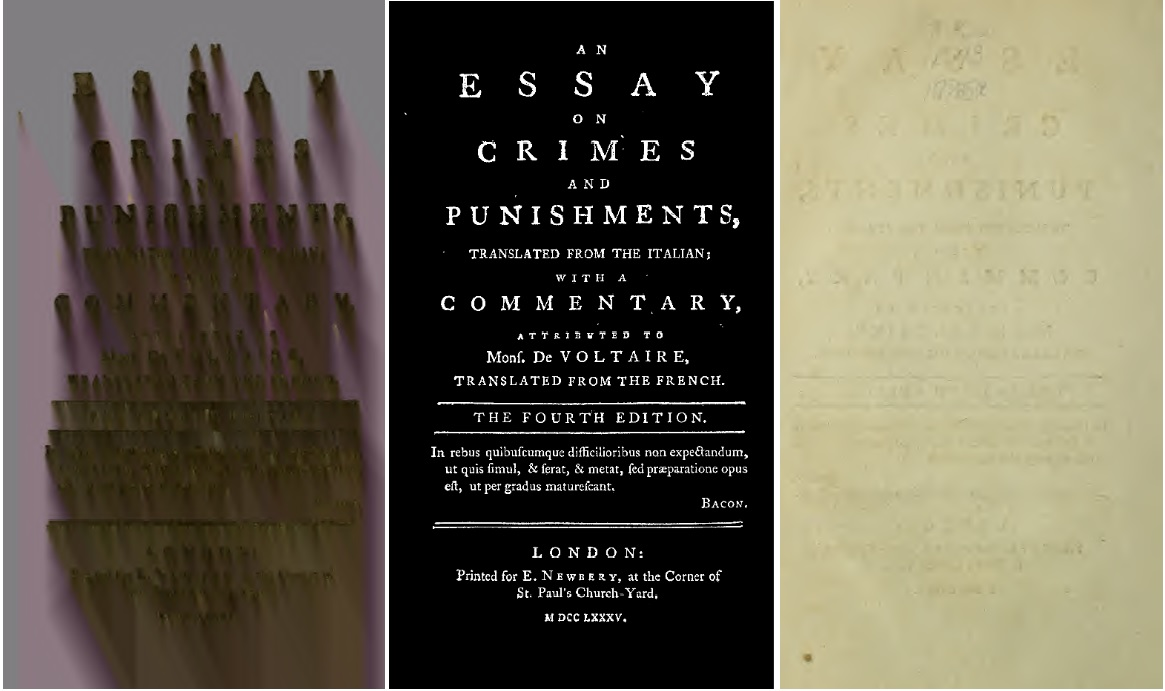
\includegraphics[width=15cm]{Partie2/images/Resultat_TIFF.jpg}
    \caption{Résultat d'une océrisation\index{OCR!ocerisation@océrisation} en \textsc{tiff} pour l'édition anglaise de 1785 du Beccaria}
    \label{fig:resultatTIFF}
\end{figure}

Dans le cas où est obtenu ce second résultat, cela pose un problème pour la suite, puisque si cela est effectivement possible de récupérer le deuxième type de production (le texte en négatif) et qu'il peut parfois être exploitable, la majorité du temps, cela s'avère peu lisible pour le script d'\acrshort{ocr}\index{OCR}, qui ne sait pas exactement ce qu'il est censé aller chercher et les résultats sont généralement assez mauvais et inutilisables.
\begin{figure}[p]
    \centering
    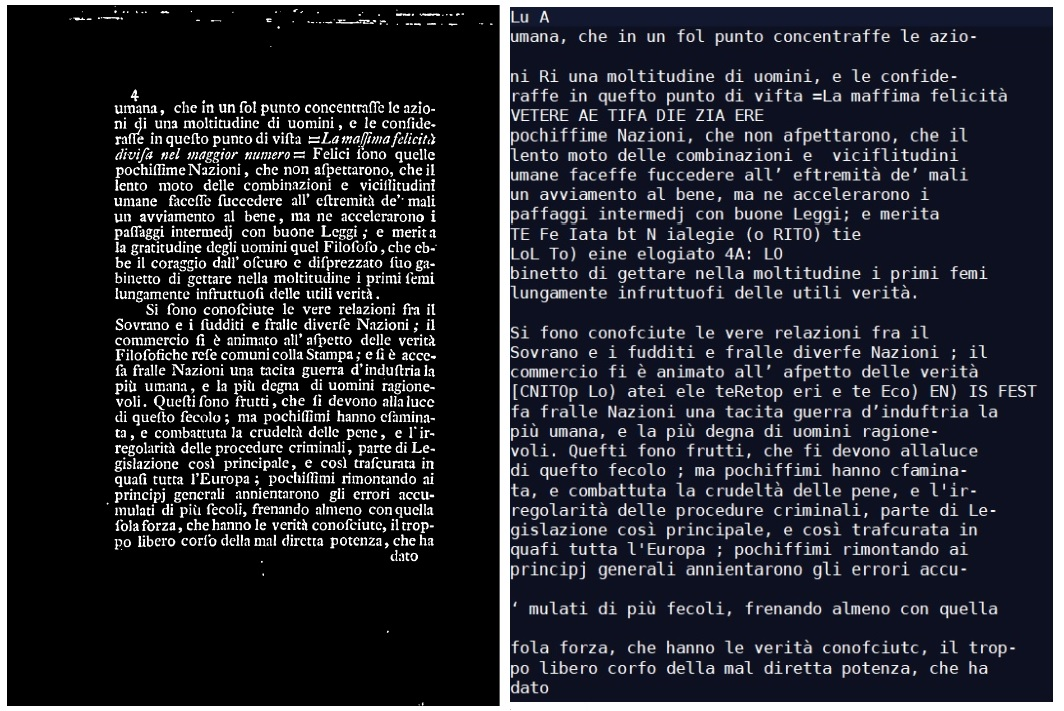
\includegraphics[width=15cm]{Partie2/images/BadTranscript_TIFF.jpg}
    \caption{Mauvaise transcription de texte, dû à l'aspect de l'image numérisée}
    \label{fig:badtranscript}
\end{figure}
Lorsque ce cas se présente, comme dans la figure \ref{fig:badtranscript}, il est donc nécessaire de produire les fichiers dans un format \textsc{jpeg}, en espérant que le document soit assez lisible pour l'\acrshort{ocr}\index{OCR} et qu'il produise un meilleur texte que le négatif du \textsc{tiff}.

Pour faire cette transformation, j'ai utilisé l'application \emph{\textsc{pdf} to \textsc{jpeg}}, qui est un convertisseur Windows, où il suffit de lui donner le fichier d'entrée, soit le fichier \textsc{pdf} à convertir, de lui donner un lieu de sortie, soit le dossier où il devra ranger les pages converties en \textsc{jpeg}. Ensuite, nous lui faisons convertir et l'opération dure entre 30 secondes et 3 minutes. Cette technique est aussi pratique que celle du \emph{PDFImages}, bien qu'elle ne soit disponible qu'en \textsc{jpeg} et seulement sur Windows. L'image est tout de même réduite et perd de la qualité, comme cela s'observe en essayant de l'agrandir pour avoir une meilleure résolution. Nous voyons que cela est très limité pour les \textsc{jpeg}, alors que cela peut se faire beaucoup plus facilement avec les \textsc{tiff}. Cela reste une option à avoir, puisque lors de la correction de la transcription, il peut être essentiel, dans le cas d'un caractère un peu effacé ou d'un mot difficile à lire, d'agrandir l'image pour mieux voir ce qui est écrit.

\paragraph{} Le \textsc{jpeg} est donc plus limité que le \textsc{tiff} pour la lecture et l'utilisation de fichiers et même s'il est utilisé pendant notre démarche, il donne lieu à un travail plus long dans la correction de la transcription puisque cela demande de corriger plus d'éléments dans le texte et d'être encore plus précis que d'habitude. De plus, le \textsc{jpeg} est plus problématique à utiliser que le \textsc{tiff}, car il n'est pas compatible, sur la plupart des ordinateurs, avec \emph{ScanTailor}, outil qui aura une fonction notable avant l'océrisation\index{OCR!ocerisation@océrisation} pour les fichiers \textsc{tiff}.

\section{Étape intermédiaire~: nettoyer ses images pour un meilleur fichier source}
Lorsque nos chapitres sont composés de fichiers avec une extension \textsc{tiff}, nous avons la possibilité d'effectuer une étape intermédiaire, qui permet d'améliorer le fichier qui sera soumis au script python pour océriser les images.

Les images en \textsc{tiff} peuvent être nettoyées partiellement à l'aide d'un logiciel~: \emph{ScanTailor}. Cette application se compose de multiples options pour pouvoir manipuler l'image et la rendre plus claire et mieux lisible par le processus d'océrisation\index{OCR!ocerisation@océrisation}. Le nettoyage se déroule en cinq étapes (la cinquième comptant elle-même plusieurs manipulations). L'image peut être scindée, dans le cas où il y a deux pages ensemble et que nous ne voulons avoir qu'une page à traiter individuellement pour la suite~; puis elle peut être redressée, dans le cas où l'écriture n'est pas droite et le texte doit être quelque peu relevé ou descendu~; ensuite, se choisit le contenu que nous voudrons faire lire par la suite. Dans un cas où nous ne voulons pas tout le texte présent sur la page mais seulement un extrait, il est possible de sélectionner ce contenu précis et à la fin, le logiciel supprimera le reste sur la page manipulée. Par la suite, nous pouvons définir les marges et enfin, la cinquième étape sera celle de la sortie. L'application produit l'image telle que nous lui avons demandée de nous la présenter durant toutes les étapes présentées et il est encore faisable d'effectuer certaines modifications. L'image est produite directement en noir et blanc, mais il est possible de revenir à la version précédente avec la coloration originale de la page. Le noir et blanc est pratique notamment car il permet d'être mieux lu par l'\acrshort{ocr}\index{OCR}. Nous pouvons également décider d'augmenter le niveau d'encre pour l'écriture, ce qui est une option utile dans le cas où le texte est un peu effacé (ce renforcement donnera la possibilité de lire certains mots peu ou non apparents précédemment). Enfin, avec cette sortie, peut également s'utiliser une fonction \og~balayage~\fg{} qui nettoie notre page, c'est-à-dire qu'elle enlève les points présents sur les pages, les ratures, ou les dégradations un peu voyantes du papier. Cela a tout de même une limite puisque l'option de balayage est disponible en plusieurs niveaux et parfois, les niveaux les plus élevés enlèvent des éléments nécessaires, comme les numéros de page ou même parfois des bouts de texte.

Les images modifiées par cette application ressortent ainsi plus claires, débarrassées de presque tout ce qui pouvait entraver la bonne lecture et la bonne transcription des caractères et donc le fichier est prêt pour être océrisé et ainsi produire un texte brut.

\section{Étape finale~: océrisation et nettoyage du texte}
Une fois toutes les manipulations faites pour obtenir une image unique numérisée avec une extension exploitable par un logiciel \acrshort{ocr}\index{OCR} et plus ou moins nettoyée pour un meilleur usage, la transcription pour produire un fichier texte peut s'effectuer, qui nous donnera, une fois tous les fichiers texte réunis et nettoyés, un chapitre complet transcrit.

\subsection{Préparer l'OCR~: installation et programmation de \emph{Tesseract}}
\subsubsection{Choisir son module d'OCR}
Le processus d'océrisation\index{OCR!ocerisation@océrisation} est aujourd'hui très répandu, pour de très nombreux types d'utilisation. Cette expansion de la méthode a permis la création de très nombreux logiciels d'\acrshort{ocr}\index{OCR}, disponibles en open source, comme \emph{Kraken}, \emph{Calamari} ou \emph{Tesseract}, ou non, pour des sources matérielles courtes ou inversement de très longs documents comme \emph{Google Cloud Vision} ou \emph{Microsoft Azure Computer Vision} et qui peuvent avoir un usage professionnel ou personnel. Des études ont été faites pour démontrer les différences entre ces logiciels et savoir lesquels fonctionnent le mieux en fonction de l'utilisation faite ou de la source matérielle{\footnote{\url{https://source.opennews.org/articles/so-many-ocr-options/ }}}.

Dans le cas de nos travaux, nous avons décidé d'utiliser \emph{Tesseract}{\footnote{\url{https://github.com/tesseract-ocr/tesseract}}} pour océriser les nouveaux chapitres du \textit{Traité}\index{Traite des delits et des peines@Traité des délits et des peines} de Beccaria. \emph{Tesseract} a l'avantage d'être open source et surtout d'être utilisable en ligne de commande (nous avons donc la possibilité de l'utiliser avec Python, notre outil de programmation depuis le début du travail). De plus, \emph{Tesseract} est très bien documenté sur sa page Github et il est donc possible d'installer tout ce qui est nécessaire, et notamment des spécificités, qui vont être nécessaires dans le cas de nos transcriptions de Beccaria. Ces spécificités sont notamment indispensables car \emph{Tesseract} fait partie des logiciels d'\acrshort{ocr}\index{OCR} qui n'ont pas de modèles préexistants dans sa programmation. Il faut donc les installer en plus de l'installation du logiciel \emph{Tesseract}. Nous utilisons \emph{Tesseract} avec \emph{PIL (Python Imaging Library)}, une bibliothèque de traitements d'images (faisant partie des librairies Python), qui permet un accès rapide aux données contenues dans une image et pour plusieurs types d'extensions d'images.

\subsubsection{Installer le logiciel \emph{Tesseract}}
Une fois le logiciel choisi, il suffit de suivre les instructions inscrites sur le Github pour installer \emph{Tesseract}. Étant sur un terminal Linux, il suffit de taper la commande \textit{\og~sudo apt install tesseract-ocr~\fg{}} et le logiciel est installé mais pas encore prêt pour utilisation. En effet, il est nécessaire, pour que \emph{Tesseract} fasse ce qui lui est demandé, d'installer également les langues à traiter avec l'\acrshort{ocr}\index{OCR}. Dans notre cas, cela sera l'italien, le français, l'anglais et l'allemand et nous devrons donc installer quatre langues sur \emph{Tesseract}. En réalité, cinq installations sont nécessaires pour avoir tous les éléments d'une bonne océrisation\index{OCR!ocerisation@océrisation}.

Tout d'abord, s'installera l'italien, le français et l'anglais, qui ne posent aucun problème~:
\begin{itemize}
    \item sudo apt install tesseract-ocr-ita (italien)
    \item sudo apt install tesseract-ocr-fra (français)
    \item sudo apt install tesseract-ocr-eng (anglais)
\end{itemize}
Il faudra cependant faire deux installations pour l'allemand~:
\begin{itemize}
    \item sudo apt install tesseract-ocr-deu
    \item sudo apt install tesseract-ocr-frk
\end{itemize}
Nous installons l'allemand standard, qui sera utile pour quelques traductions mais également l'allemand \emph{fraktur}, qui aura la possibilité de reconnaître, pendant l'océrisation\index{OCR!ocerisation@océrisation}, qu'il n'est pas en présence d'un texte allemand écrit de manière standard mais d'un texte allemand rédigé avec l'écriture \emph{fraktur}, plus difficile à reconnaître et à lire qu'un alphabet standard. Cela implique donc que \emph{Tesseract} doit être programmé pour pouvoir reconnaître ces caractères, sinon il est très probable qu'il ne sache lire que très difficilement les textes lorsqu'ils sont écrits ainsi. Il est possible par la suite, installer d'autres langues, dans le cas où des traductions d'éditions dans d'autres langues sont découvertes et insérées dans notre projet.

\subsection{Application du script d'OCR}
Nous avons deux scripts \acrshort{ocr}\index{OCR}, un pour l'extension \textsc{tiff} et un pour l'extension \textsc{jpeg}, mais ils ne sont pas fondamentalement différents, seul un élément change entre les deux impactant ainsi leur mode de fonctionnement. Le script est rédigé de manière à ce que l'invite de commande aille chercher les images, les lise, en extrait le texte qu'il visualise et l'inscrit dans un nouveau document ayant le même nom que l'image qu'il traite mais avec une extension \textsc{txt}.
\begin{figure}[t]
    \centering
    \fbox{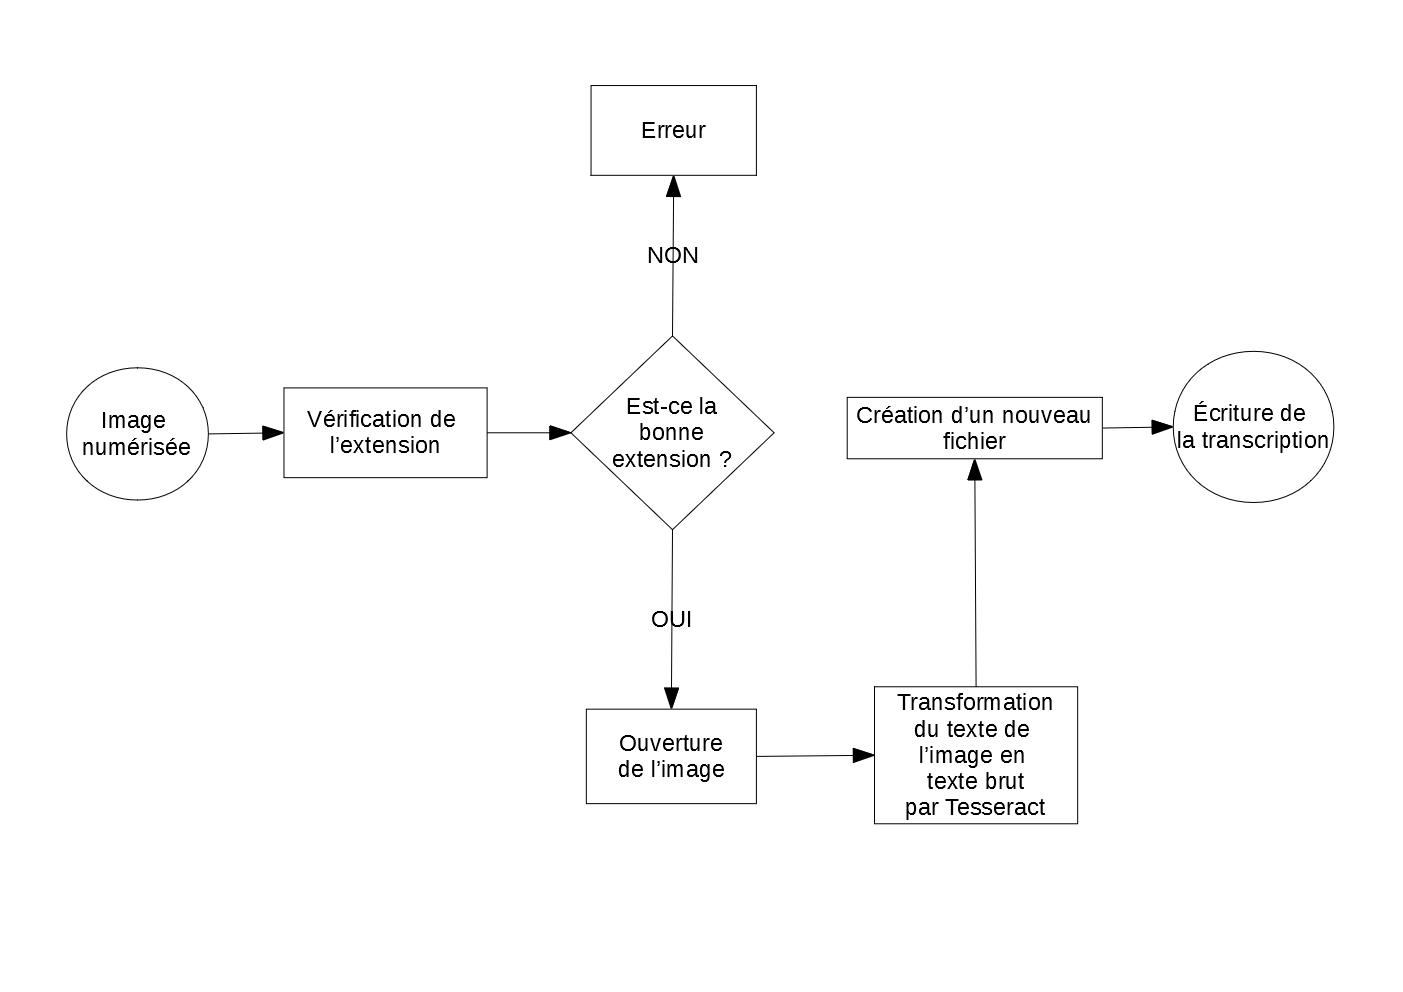
\includegraphics[width=16cm]{Partie2/schemas/OCR.jpg}}
    \caption{Étapes de la transcription, d'une image numérisée à un fichier texte brut}
    \label{fig:OCR}
\end{figure}
La différence entre \textsc{tiff} et \textsc{jpeg} est le fait que nous demandons à l'invite de commande d'aller chercher les images numérisées et il est spécifié dans le script que pour reconnaître la source matérielle, le terminal doit trouver une extension définie pour savoir quel document traiter, et c'est donc à la première ligne de la boucle \textit{for} que s'effectue le changement~:
\begin{itemize}
    \item \mint{python}{if i.endswith("jpg"): (pour ocr_jpg.py)}
    \item \mint{python}{if i.endswith("tif"): (pour ocr_tiff.py)}
\end{itemize}
Ainsi, avec cette différence, nous pouvons traiter soit les images qui sont passées sans problème par la conversion en \textsc{tiff}, soit celles qui ont dû passer par le convertisseur \textsc{jpeg}. Dans les deux cas, et notamment le second, la transcription n'est pas parfaite, ou même parfois assez mauvaise et il est donc nécessaire de la corriger manuellement.

\subsection{Correction manuelle du fichier texte}
Le processus d'\acrshort{ocr}\index{OCR} n'est pas un processus parfait puisque la source même que nous lui soumettons n'est pas parfaite et l'\acrshort{ocr}\index{OCR} retranscrit mot à mot, autant qu'il peut, ce qui lui est dit mais il n'effectue généralement pas de traitement a posteriori pour corriger les possibles erreurs. Il n'y a aucune réflexion pendant le processus et ce sera donc à nous d'aller ensuite corriger au mieux ce qu'il a proposé. Le travail de correction reste cependant assez simple, voire parfois redondant, puisque les éditions par langue sont majoritairement les mêmes à quelques mots ou phrases près, donc lorsque nous avons corrigé un texte, les suivants présentent à peu près les mêmes fautes, l'\acrshort{ocr}\index{OCR} ne sachant pas transcrire les mêmes éléments d'un texte à l'autre.

Ensuite, nous retrouvons des éléments assez récurrents à corriger~: tout d'abord,  dans les textes entre 1760 et 1780, la graphie du \textit{s} n'a pas toujours sa graphie habituelle, puisqu'il ressemble parfois à un \textit{f} plutôt qu'à un \textit{s}, il est la représentation d'un \textit{s} long, qui se retrouvent à de très nombreuses reprises dans les textes. Le logiciel d'\acrshort{ocr}\index{OCR} ne connaît cependant pas cette lettre et l'identifie donc comme un \textit{f} et ce sera donc à nous d'aller corriger cela, en se fiant au mot de base et lorsque cela n'est pas sûr, en se fiant au contexte et à la formulation de la phrase, pour savoir si c'est un \textit{s} ou un \textit{f}. \newline
Par la suite, il est peut être nécessaire de corriger des mots que l'\acrshort{ocr}\index{OCR} n'a pas bien lu, notamment dû aux difficultés de jambages entre le u, le n ou le m ou des différences entre un l, un f et un i dont la barre et le point ont été trop collés. Il y a même certains cas de points-virgules qui ont été confondus avec des lettres ou inversement.

Ces occurrences sont les plus régulières et surtout les plus simples mais il y a aussi des cas où le logiciel n'a pas du tout reconnu une ligne de caractères et donc laisse une ligne de vide ou même une liste de caractères sans aucun sens, comme cela peut se voir sur la figure \ref{fig:badtranscript}. Dans ces cas-là, il est donc nécessaire de réécrire à la main la phrase en entier en suivant les fins de lignes et les séparations de mots.

Parmi les autres problèmes mineurs de transcription, le logiciel d'\acrshort{ocr}\index{OCR} est généralement perturbé par les dessins et autres fioritures qui se trouvent en début de chapitre majoritairement et qu'il faut donc supprimer dans le fichier texte, notamment lorsque cela a été transcris par plein de petits signes incohérents.

La correction manuelle demande donc de l'attention et prend un certain temps, pour obtenir alors un texte correct et lisible. L'erreur étant humaine, il est toujours possible que le texte présente des fautes, mais puisque ces textes seront généralement utilisés par la suite pour un alignement\index{Alignement} et des analyses de statistiques textuelles, ils seront manipulés par des scripts que nous présenteront ensuite et donc les erreurs assez évidentes qui resteraient seront corrigées par certains des scripts.

\section*{Conclusion~: un processus adapté à la source ?}
\addcontentsline{toc}{section}{Conclusion~: un processus adapté à la source ?}
La préparation et la réalisation de l'\acrshort{ocr}\index{OCR} des textes prennent un certain temps et il est tout de même nécessaire par la suite d'opérer des modifications dans le texte, le logiciel n'étant pas fiable à 100\%. Il est donc pertinent de se demander si \emph{Tesseract} est la solution la plus efficace et la plus effective pour nos documents. Nous pourrions nous tourner vers d'autres logiciels \acrshort{ocr}\index{OCR}, open-source mais non en Python ou de bureau, avec un coût en fonction du nombre de pages océrisés, pour espérer ainsi avoir un meilleur résultat.

Mais, s'il est vrai que \emph{Tesseract} n'offre pas toujours des résultats très probants pour les textes traduits en \textsc{jpeg} car pas assez lisible, qu'il se trompe même dans les cas où l'image a été nettoyée et qu'il rencontre parfois quelques autres petits problèmes, il reste toutefois pertinent vis-à-vis de notre source. Si le texte de Beccaria était beaucoup plus volumineux, s'il était écrit avec une graphie beaucoup moins standard ou sur des pages avec des lignes très fines et une grande quantité de textes, comme cela peut être le cas pour des manuscrits médiévaux par exemple, il serait logique d'utiliser certains des logiciels que nous avons mentionné plus tôt, qui opèrent sur des plus grandes quantités de texte ou certains plus précis qui se concentrent sur certains textes, comme \emph{Transkribus} qui travaille sur de l'écriture manuscrite. Notre source ne possède aucune de ces particularités et ne nécessite que des transcriptions par six à douze pages, avec des images généralement de bonne qualité et les inconvénients donc de corrections et nettoyage à faire sont assez mineurs pour pouvoir rester sur le module \emph{Tesseract} pour l'océrisation\index{OCR!ocerisation@océrisation} de nos documents, et ainsi produire la source telle quelle.
\chapter{\label{chap_mise_en_forme}Transformer et nettoyer le texte pour une analyse adaptée à nos objectifs}
\fancyhead[LO, RE]{Mettre en forme le texte}

\section{Mettre en forme la transcription}
\subsection{Pourquoi mettre en forme la transcription}
Après avoir récupéré la version océrisée des chapitres que nous étudierons par la suite, un premier nettoyage visuel a été fait, pour que l'information du fichier texte corresponde à ce qu'il y a dans le manuscrit et donc pour corriger les possibles erreurs qui sont apparues lors de la transformation du chapitre en une version texte. Une fois cela effectué, nous avons donc un fichier texte qui ressemble trait pour trait à la structure dans les différentes pages du manuscrit, ce qui permet ainsi d'avoir un document conforme si nous souhaitons simplement faire une reproduction exacte du manuscrit en version texte à étudier tel quel.

Cependant, pour la plupart des analyses et recherches à faire sur les chapitres du Beccaria, la forme du texte ne nous intéresse pas. L'analyse tend à se porter plutôt sur le fond, puisque le but du projet est de créer un dictionnaire de mots du droit et ainsi donc, étudier le contenu du texte et les mots utilisés. Dans un objectif plus proche, nous voulons principalement faire de l'alignement\index{Alignement} avec les différents chapitres, pour voir les changements (remplacements, insertions, suppressions) que les multiples éditeurs ont pu effectuer, et si certains de ces changements peuvent être une coupure de phrase ou un déplacement de paragraphes (pertinent pour notre analyse), d'autres éléments du texte ne nous intéressent pas et pourraient même fausser notre analyse. Nous entreprenons alors de mettre en forme le texte en écrivant un script Python qui sera adapté à toutes les versions du Beccaria et à toutes les éditions des chapitres, pour nettoyer et ménager un maximum d'informations.

\subsection{Réflexions sur les éléments à mettre en forme}
Il est nécessaire ensuite de s'interroger sur les éléments à traiter pour les voir disparaître ou changer et ainsi, faciliter au maximum notre analyse pour la suite du travail.

Le point le plus important à traiter était celui des coupures de mots. En effet, les manuscrits de l'époque n'offrant pas de très longs espaces pour écrire les textes, il y a de nombreux mots séparés par un tiret et une mise à la ligne. Ceux-ci représentent la correction la plus importante, puisque la méthode ou la taille d'écriture, la place allouée pour un chapitre ou l'espace de la feuille n'étaient pas toujours les mêmes en fonction du manuscrit et donc ce ne sont jamais les mêmes mots qui sont séparés en fonction des textes, mais lors des diverses analyses, ces mots sont considérés comme des différences entre deux versions ou ne sont pas comptés dans une analyse de correspondances, ce qui représente donc une grande marge d'erreur pour l'étude des texte.

Ensuite, de la même manière qu'avec les mots coupés par un tiret, le texte est segmenté en de très courtes lignes, qui ne permettent pas d'apprécier complètement les blocs de texte qui peuvent être similaires entre deux versions et il était donc nécessaire de faire également disparaître ces sauts de lignes, pour créer des paragraphes plus compacts. Un problème se pose cependant à ce stade de la réflexion, puisque nous ne souhaitons pas voir disparaître tous les sauts de lignes. Beccaria a décidé, lorsqu'il a rédigé son texte, de faire des séparations de paragraphes qui expriment sa pensée et sa manière de réfléchir. Cela a été repris par les éditeurs ou changé par d'autres, mais dans les deux cas, la place des paragraphes a une importance pour l'analyse du texte et nous allons donc chercher à conserver ces séparations, qui seront utiles notamment lors de la procédure d'alignement\index{Alignement}, pour réaliser un alignement\index{Alignement} par paragraphe. Il y a donc deux manières différentes d'appréhender la séparation du texte dans le script Python, ce qui a causé une certaine difficulté, comme cela s'observera par la suite.

Le troisième point auquel nous avons réfléchi était l'idée de supprimer des éléments plus mineurs qui auraient pu gêner dans l'analyse textuelle, tels que les majuscules, certains signes de ponctuations ou encore quelques symboles à régulariser. Après avis des membres du projet et notamment des linguistes, nous avons conclu de les garder, car cela n'empiétait pas sur l'analyse que nous effectuerons. Le seul élément mineur que nous avons décidé de supprimer est le numéro des pages présent pour montrer exactement la disposition dans le manuscrit~: l'élément nuit à la bonne lecture de notre document et n'est plus nécessaire avec la nouvelle mise en forme apportée au texte. Ainsi, le cahier des charges du script de mise en forme est établi et nous pouvons passer à la rédaction.

\subsection{Représentation de la mise en forme des transcription}
\begin{figure}[p]
    \centering
    \fbox{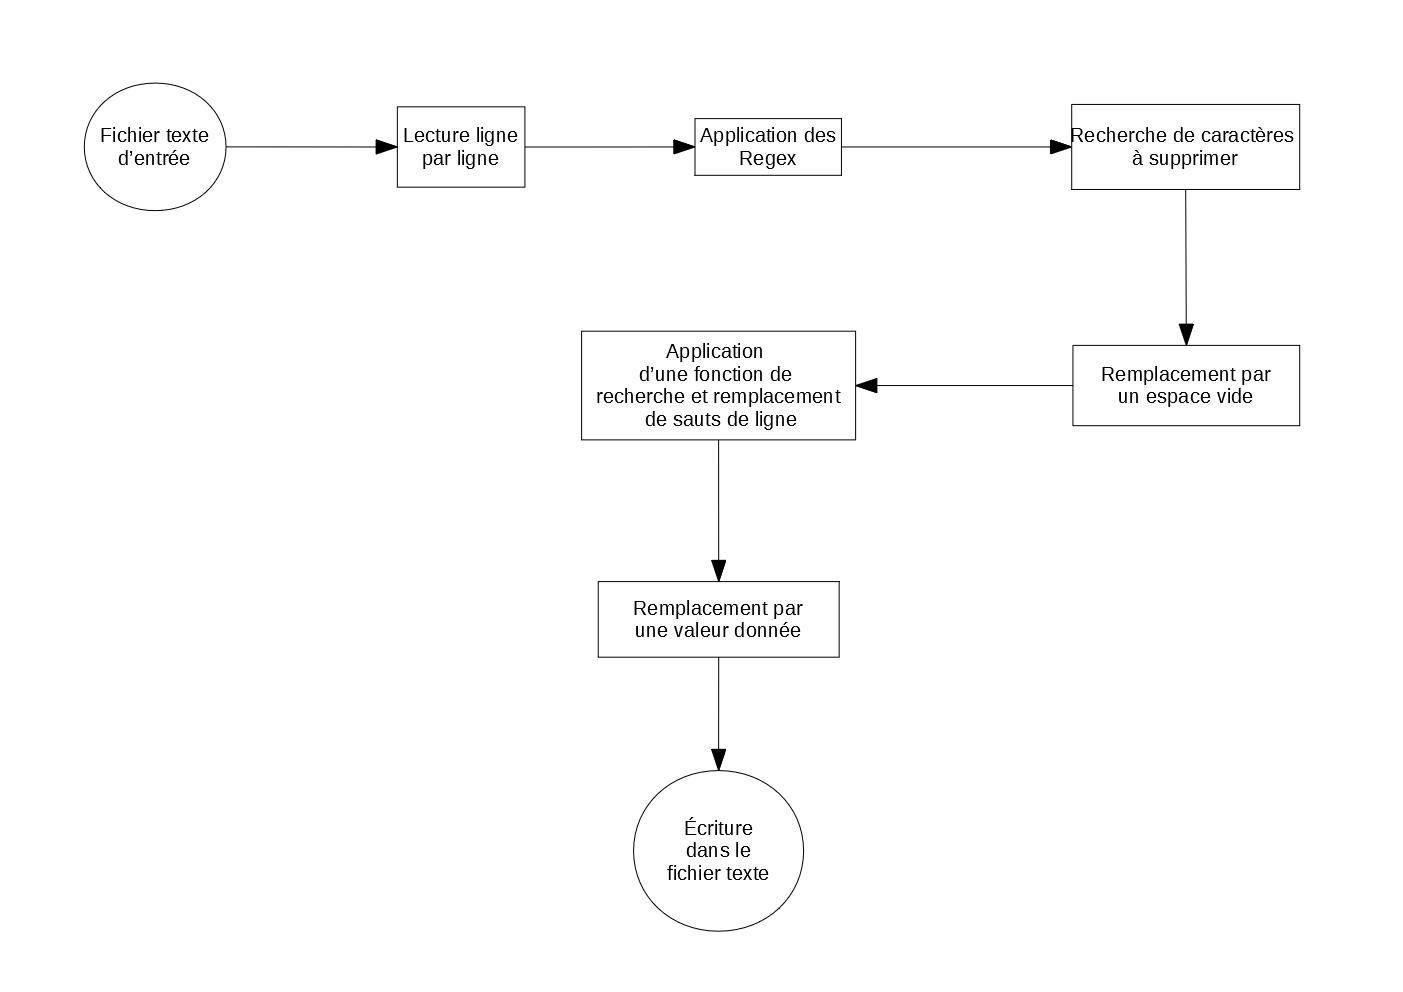
\includegraphics[width=14cm]{Partie2/schemas/3_mise_en_forme_bis.jpg}}
    \caption{Diagramme d'activité représentant les étapes pour mettre en forme les fichiers texte de transcription}
    \label{fig:etape3}
\end{figure}
Le diagramme d'activité de la figure \ref{fig:etape3} présente un traitement qui a pour objectif de partir d'un fichier d'entrée, soit la transcription directe du manuscrit pour arriver à un fichier de sortie qui sera la mise en forme souhaitée de ce texte. Ce processus lit le texte ligne par ligne pour trouver les éléments qu'il devra corriger. Il effectue ensuite deux tâches, il va tout d'abord, à l'aide d'expressions régulières, supprimer certains éléments du texte définis plus tôt, soit les numéros de pages et les tirets en fin de ligne, pour les remplacer par un simple espace. Ensuite, à l'aide d'une fonction de recherche et remplacement de sauts de ligne, ce traitement supprime les sauts de ligne inutiles tout en conservant les sauts de ligne qui correspondent à la fin d'un paragraphe et au début d'un autre. Une fois cela effectuée, la version mise en forme du texte est intégrée dans un fichier texte de sortie.
\begin{figure}[p]
    \centering
    \fbox{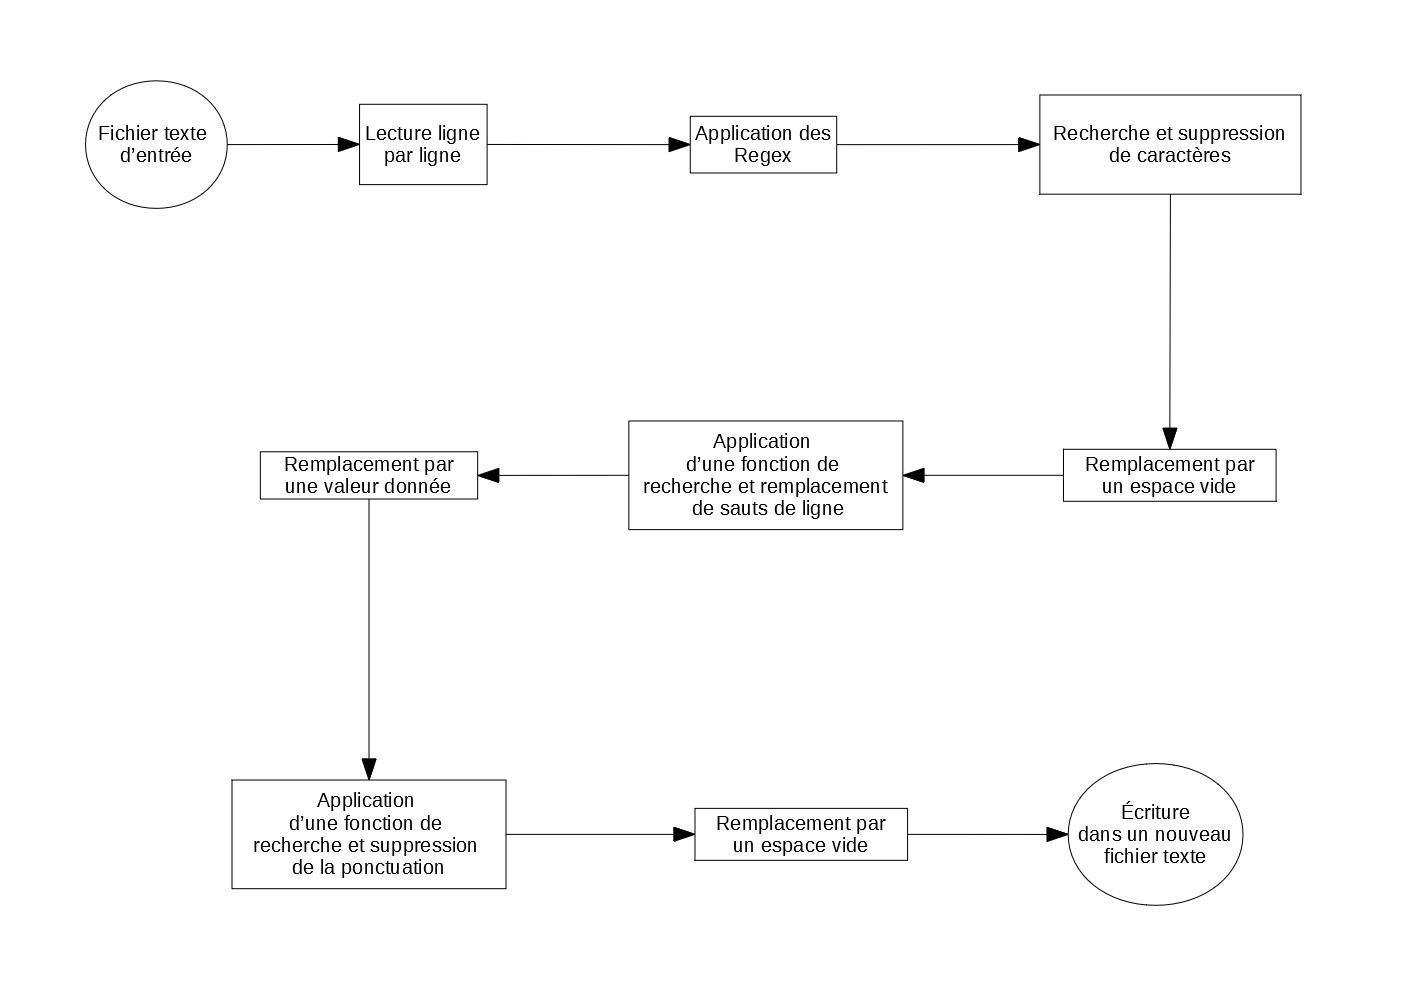
\includegraphics[width=14cm]{Partie2/schemas/1_mise_en_forme.jpg}}
    \caption{Diagramme d'activité représentant les étapes pour mettre en forme la transcription texte ainsi que supprimer des éléments de ponctuation.}
    \label{fig:etape1}
\end{figure}
Il y a dans le diagramme de la figure \ref{fig:etape1} les mêmes éléments qu'observés dans la figure \ref{fig:etape3}, mais une étape ici a été rajouté, celle de supprimer la ponctuation, ce qui sera nécessaire pour faciliter le travail du vérificateur orthographique, qui sera utilisé lors de la prochaine démarche. Nous incluons donc seulement cette étape avant de réaliser la vérification orthographique. Le fichier texte de mise en forme standard qui sera utilisé par la suite sera fait en suivant les étapes du diagramme d'activité de la figure \ref{fig:etape3}.

\section{Implémentation du script Python}
\subsection{Ajout des modules}
Nous avons commencé à réfléchir aux modules sur lesquels s'appuyer pour la rédaction et avons décidé d'utiliser majoritairement le module \emph{re} de Python. Il a pour but d'utiliser les expressions régulières, adéquat puisque notre démarche consiste à effectuer des remplacements au sein du texte. Nous avons également choisi d'utiliser le module \emph{sys} présent notamment dans les scripts d'\acrshort{ocr}\index{OCR} pour permettre de faire appel par la suite au script et aux paramètres qui seront donnés dans l'interpréteur de commande pour ainsi réaliser l'opération plus rapidement et plus efficacement. 

\subsection{Paramètres d'entrée et de sortie des fichiers}
Nous avons créé le script en premier lieu en définissant des paramètres qui ne concerneraient qu'un fichier unique, pour pouvoir tester rapidement sur un seul fichier si le script fonctionnait. Nous avons donc défini un fichier d'entrée en mode lecture et en encodage UTF-8 et un fichier de sortie en mode écriture, auxquels nous avons attribué une place pour la requête avec le terminal au moyen des \emph{sys.argv[]}. Par la suite, ces informations-là ont été retirées lorsque le script a été défini pour gérer un dossier complet de transcriptions et non juste un seul fichier. Nous avons alors importé le module \emph{os}, qui permet de manipuler des chemins pour aller chercher les fichiers qui nous intéressent dans un dossier. Nous avons ainsi inséré la fonction \emph{os.walk()} à laquelle a été ajouté un argument qui sera appelé dans la commande du terminal et qui correspondra au dossier contenant les transcriptions à normaliser. Nous avons ensuite redéfini les \emph{file\_in} et \emph{file\_out} pour qu'ils répondent à nos attentes et notamment que le fichier de sortie contienne une indication qui démontre que le document a été normalisé (\emph{sys.argv[2] + \og~/Norm~\fg{} + filename}). En fin de script, deux lignes de code permettent de fermer les deux fichiers et de clore le script.

\subsection{Boucler sur les lignes}
Après avoir paramétré le script, nous avons dû trouver un moyen de créer une boucle pour pouvoir travailler sur les lignes de texte pour effectuer les modifications nécessaires, étape observée au tout début du schéma de la figure \ref{fig:etape3}. Cette étape a donné lieu à de nombreux essais infructueux, pour trouver la technique la plus adéquate pour avoir correctement accès au contenu de notre texte. 
Notre premier essai était celui-ci~: 
\begin{minted}{python}
    for line in file_in:
\end{minted}
Nous nous sommes cependant vite rendu compte qu'une technique pareille prenait en compte le document ligne par ligne mais en les considérant comme de simples éléments détachés les uns des autres sans aucun lien, bloquant ainsi la majorité des manipulations effectuées dans le codage et n'apportant ainsi rien à notre mise en forme.

Nous avons alors tenté de trouver une manière de lire le document en plusieurs lignes liées entre elles, en utilisant plusieurs méthodes~:
\begin{itemize}
    \item \mint{python}{split_lines = line.splitlines()}
    \item \mint{python}{liste = [item for item in line.split('\n')]}
    \item \mint{python}{alltext = ' '.join(liste)}
    \item \mint{python}{for match in test.finditer(line):}
    \begin{itemize}
        \item \mint{python}{print(match.groups())}
    \end{itemize}
\end{itemize}
Cela ne correspondait jamais à ce que nous souhaitions faire ou ne donnait pas les résultats voulus pour la mise en forme. Nous avons finalement trouvé une méthode Python qui est dédiée à la lecture de lignes et notamment de plusieurs lignes (soit le texte en son entier), \emph{.readlines()}, défini ainsi par Python~:
\begin{quotation}
\og~\emph{f.readline()} lit une seule ligne du fichier~; un caractère de fin de ligne (\textbackslash n) est laissé à la fin de la chaîne. Il n'est omis que sur la dernière ligne du fichier si celui-ci ne se termine pas un caractère de fin de ligne. [...] Pour construire une liste avec toutes les lignes d'un fichier, il est aussi possible d'utiliser \emph{list(f)} ou \emph{f.readlines()}.\fg{} \footnote{Documentation Python~: 7 - Les entrées/sorties - \url{https://docs.python.org/fr/3/tutorial/inputoutput.html}}
\end{quotation}
Ainsi, avec cette méthode, le script va lire et analyser aisément les lignes, en prenant en compte certaines des informations précédant et suivant une ligne en particulier et ainsi, répondre aux attentes imposées lors de la recherche d'éléments dans le texte.

\subsection{Comment conserver la structure des paragraphes~: trouver la bonne expression régulière}
Comme cela a pu s'observer lors de la réflexion sur le script, nous voulons insérer plusieurs types d'éléments dans le code qui demandera plus ou moins de réflexions. La plupart des morceaux ne posent aucun problème, l'expression régulière correspondante n'étant pas trop difficile à trouver mais un cas en particulier pour la mise en forme a été assez ardu~: la structuration des paragraphes.

La transcription du manuscrit contenait deux types de cas pour lesquels devait s'appliquer une solution différente en fonction du cas, ce qui se présentait ainsi~:
\begin{itemize}
    \item Cas 1~: La phrase a été coupée en plein milieu et le saut de ligne doit disparaître, soit  \og~minuscule - saut de ligne - minuscule~\fg{} --> Changement en espace simple~;
    \item Cas 2~: La phrase finit par un point et est suivie d'un saut de ligne et la ligne suivante commence par une majuscule et cela doit être conservé, soit  \og~point  - saut de ligne - Début de mot avec une majuscule~\fg{} --> Conserver la mise à la ligne.
\end{itemize}
L'opération pour réaliser le cas 1 était plutôt simple puisqu'il suffisait juste de faire disparaître tous les sauts de lignes, mais dans ce cas, la structure du cas 2 est perdue. Nous avons alors cherché plusieurs types d'expressions régulières, qui répondraient à notre objectif, comme notamment signifier le cas 2 en expression régulière ( \og~.\textbackslash n[A-Z][A-Za-z] ~\fg{}) et lui dire que nous voulons conserver ce saut de ligne ou chercher à faire disparaître les sauts de ligne qui n'existent que pour le cas 1 ( \og~(.+)\textbackslash n(.+) ~\fg{}), ce qui n'a jamais donné aucun résultat concluant pour notre mise en forme.

Finalement, après réflexion, nous avons trouvé une solution mais elle implique d'effectuer trois étapes successives pour que l'objectif soit atteint et bien que le texte ne soit pas parfait ensuite, il répond au moins aux attentes pour la structure des pages.

Voilà comment se décompose la solution~:
\begin{itemize}
    \item Étape 1~: Modification du cas 2 en changeant le point de fin de phrase par un autre signe quelconque mais qui ne figure préférablement pas non plus dans le texte~;
    \item Étape 2~: Suppression de tous les sauts de ligne présents dans le texte pour obtenir un bloc compact du texte sans autre délimitation que les phrases~;
    \item Étape 3~: Réintégration des sauts de ligne là où il y a le signe de l'étape 1 et en même temps, remplacement de ce signe par le point d'origine.
\end{itemize}
Par conséquent, le texte retrouve la structuration de paragraphes que nous voulons conserver. Cependant, cette technique représente tout de même trois lignes de code pour une étape non trouvée avec une seule ligne et pour simplifier le code et permettre plus de clarté, ces étapes sont intégrées dans une fonction.

\subsection{Création des fonctions}
Si le script ne se compose pas d'un très grand nombre d'éléments, il existe certaines requêtes dans le codage qui nécessitent plus de deux à quatre lignes, ce qui peut faire lourd dans le code et notamment dans la boucle. Nous aurons alors recours à des fonctions pour donner un nom à ces étapes un peu longues et ainsi faciliter la lecture du code. Il y a deux fonctions plus ou moins complexes dans le script, dont une qui ne sera utilisée que partiellement.

\subsubsection{supprimer\_ponctuation()}
Pour mettre en forme le texte en suivant les instructions des responsables du projet, seuls les tirets et sauts de ligne, ainsi que numéros de page, doivent être supprimés. Nous ne devrons donc pas supprimer la ponctuation, nécessaire à une bonne compréhension du texte et à un souci d'authenticité vis-à-vis des auteurs ou traducteurs. En l'état, dans la version définitive du texte produite avec sa nouvelle mise en forme, la ponctuation est conservée. Cependant, une des étapes qui viendra après nécessite que la ponctuation soit supprimé et nous écrivons donc une fonction pour réaliser cela, fonction qui apparaît dans la figure \ref{fig:etape1}. Pour réaliser cela, j'ai extrait une fonction étudiée pendant les cours de Python, qui définit les signes de ponctuation à retirer et à l'aide d'une boucle \emph{for}, ils sont remplacés par du vide. J'ai modifié quelque peu le contenu de la variable ponctuation et j'y ai fait apparaître les différentes variantes de l'apostrophe ainsi que les points et j'ai retiré les tirets, car ils sont nécessaires à la compréhension de certains mots du texte. Une fois la fonction définie, elle est insérée dans les lignes de code de la boucle \emph{for} avec notre texte comme paramètre.

\subsubsection{mise\_a\_la\_ligne()}
Cette fonction reprend ce qui a été vu plus tôt dans notre réflexion pour conserver la structure du texte. Nous insérons donc dans cette fonction, à laquelle nous mettons comme paramètre un texte, les trois lignes de code pour conserver les paragraphes. Nous pouvons ensuite l'introduire dans notre boucle \emph{for} et limitons ainsi la longueur du code tout en ayant défini une fonction qui peut être réutilisée par la suite.

\section{Rédaction du script}
Le script est presque fait, tous les éléments nécessaires ont été définis et il faut maintenant écrire les lignes de code dans la boucle \emph{for} et nous suivons alors un certain cheminement pour entrer chaque ligne nécessaire pour le code.

Tout d'abord, les numérotations de pages sont supprimées car inutiles pour l'analyse du texte en lui-même. Ensuite, les mots séparés d'un tiret sont régularisés, car écrits ainsi pour le manuscrit et lors de l'océrisation\index{OCR!ocerisation@océrisation}, en supprimant le tiret et le saut à la ligne. Nous ajoutons également une variante, nécessaire pour les éditions allemandes, puisqu'il y a parfois le caractère  \og~=~\fg{} au lieu d'un tiret. Puis, une de nos fonctions est insérée, celle pour structurer les paragraphes. Enfin, la dernière fonction, définie dans le cas de l'utilisation du script pour la première étape de la vérification orthographique est appelée, soit la fonction pour supprimer les caractères de ponctuation à faire disparaître.

\section*{Conclusion~: application du script}
\addcontentsline{toc}{section}{Conclusion~: application du script}
Après application du script sur le chapitre utilisé comme exemple pour l'élaboration, nous pouvons observer le rendu. La structure du texte a été conservée, mais il y a néanmoins des coquilles. Certains mots n'ont pas été recollés correctement (du fait de leur séparation de base par un tiret et par le numéro de page) et beaucoup d'espaces non voulus sont également présents dans le texte, notamment au niveau des délimitations de paragraphes. La plupart de ces erreurs peuvent être corrigées par la suite à la main, sans que cela soit trop compliqué ou long, pour permettre ainsi d'avoir un texte répondant à toutes nos exigences pour l'analyse future.
Le script de mise en forme permet donc de présenter notre texte comme nous le souhaitions et nous pourrons, par la suite, l'appliquer aux chapitres suivants.
\chapter{Établir une correction orthographique et une annotation linguistique semi-automatique}
\fancyhead[LO, RE]{Obtenir une version propre et finalisée du texte}

\section{Quelles corrections du texte ?}
Notre objectif est de procéder à une analyse des chapitres du Beccaria, et notamment observer le lexique utilisé et les termes juridiques qui ont été employés pour mener à la création du dictionnaire métalexicographique. Ainsi, si nous avons écrit un script pour permettre de mettre en forme les fichiers textes et alors, avoir une matière plus homogène pour l'analyse, il reste tout de même après cela des modifications à réaliser.

En effet, le texte contient un certain nombre de fautes qui sont dues à de multiples éléments~: erreurs lors de la transcription après océrisation\index{OCR!ocerisation@océrisation}, fautes créées par la mise en forme du texte (mots toujours coupés en deux ou tirets enlevés alors que nécessaires) et surtout des erreurs inhérentes à l'époque d'écriture des textes, tel que le verbe \textit{paraître} qui s'écrit \textit{paroître} ou le mot \textit{temps} qui s'écrit \textit{tems}. Si les deux premières ne posent pas trop de problème et peuvent être facilement corrigées, la dernière a demandé plus de réflexions, pour savoir si, dans le principe d'homogénéisation décidé, certains des verbes, noms et adjectifs présents dans le texte doivent être modernisés. Nous avons décidé de ne pas modifier l'écriture des mots dans un souci d'authenticité du texte, mais de tout de même les extraire, pour les ajouter, par la suite, dans un logiciel de statistiques textuelles (choix de \textsc{txm} pour ce projet), pour leur permettre de reconnaître la forme du verbe si elle leur est inconnue.\pagebreak

Une fois ces réflexions faites et le choix de corrections effectué, nous pouvons commencer à manipuler les fichiers textes à l'aide de plusieurs scripts (quatre sont nécessaires pour avoir une version du texte finalisée) qui changeront le texte typographiquement et orthographiquement, notamment à l'aide d'un module Python spécialisé dans la correction orthographique.

\section{Le module \emph{pyspellchecker}~: une vérification quasi automatique de l'orthographe}
Pour opérer les corrections dans le texte, le choix s'est porté sur un module développé pour Python pour faire de la vérification orthographique \footnote{\emph{Pyspellchecker}~: \url{https://github.com/barrust/pyspellchecker}}. Comme tous les modules Python, il peut s'installer sur l'ordinateur à l'aide d'un \emph{pip install} et donne ensuite accès aux différentes méthodes proposées pour effectuer des corrections.

Le module fonctionne avec de multiples langues (le français, l'allemand, l'anglais, l'espagnol et le portugais sont présents dans le module lors de l'installation) à l'aide d'un dictionnaire de fréquences de mots, qu'il est possible d'améliorer en le complétant avec les mots qu'il n'aurait pas reconnu lors de l'utilisation ou même en ajoutant une nouvelle langue à l'aide d'un dictionnaire de mots d'une autre langue qui est exporté et rattaché au module.

Ensuite, en se basant sur ces dictionnaires, le module a la possibilité d'afficher plusieurs types d'informations. Tout d'abord, en lui soumettant un texte, il peut, à l'aide de la méthode \emph{.unknown()} afficher les mots erronés qu'il a trouvé dans le texte et ensuite, nous obtenir par exemple des corrections de deux manières~:
\begin{itemize}
    \item \emph{spell.correction()} --> cela fera apparaître la correction que le vérificateur orthographique considère la plus appropriée~;
    \item \emph{spell.candidates()} --> le vérificateur orthographique présentera les solutions qu'il considère les plus proches du mot erroné.
\end{itemize}
D'autres éléments sont à disposition avec ce module, tel que l'inverse de la méthode \emph{.unknown()}, soit \emph{.known()} qui fait apparaître dans une liste les mots que le dictionnaire a reconnu dans le texte. Nous pouvons également lui demander la fréquence d'un mot choisi à l'aide de \emph{.word\_probability()}, ce qui permettrait par exemple d'en apprendre un peu plus sur le contenu des dictionnaires de fréquences.
Le module de vérification orthographique propose donc de multiples moyens de corriger un texte, en faisant apparaître des informations différentes en fonction de nos recherches et nous avons donc utilisé certaines de ces méthodes, mêlées à des boucles, pour pouvoir effectuer nos corrections de texte.

\section{Opérer des modifications dans le chapitre~: une intervention en plusieurs étapes}
Une fois que sont établies les corrections à réaliser et ce qui sera utilisé pour le faire, nous pouvons mettre en place le processus pour modifier les chapitres et obtenir nos versions finalisées qui seront utilisées pour l'analyse.
\begin{figure}[H]
    \centering
    \fbox{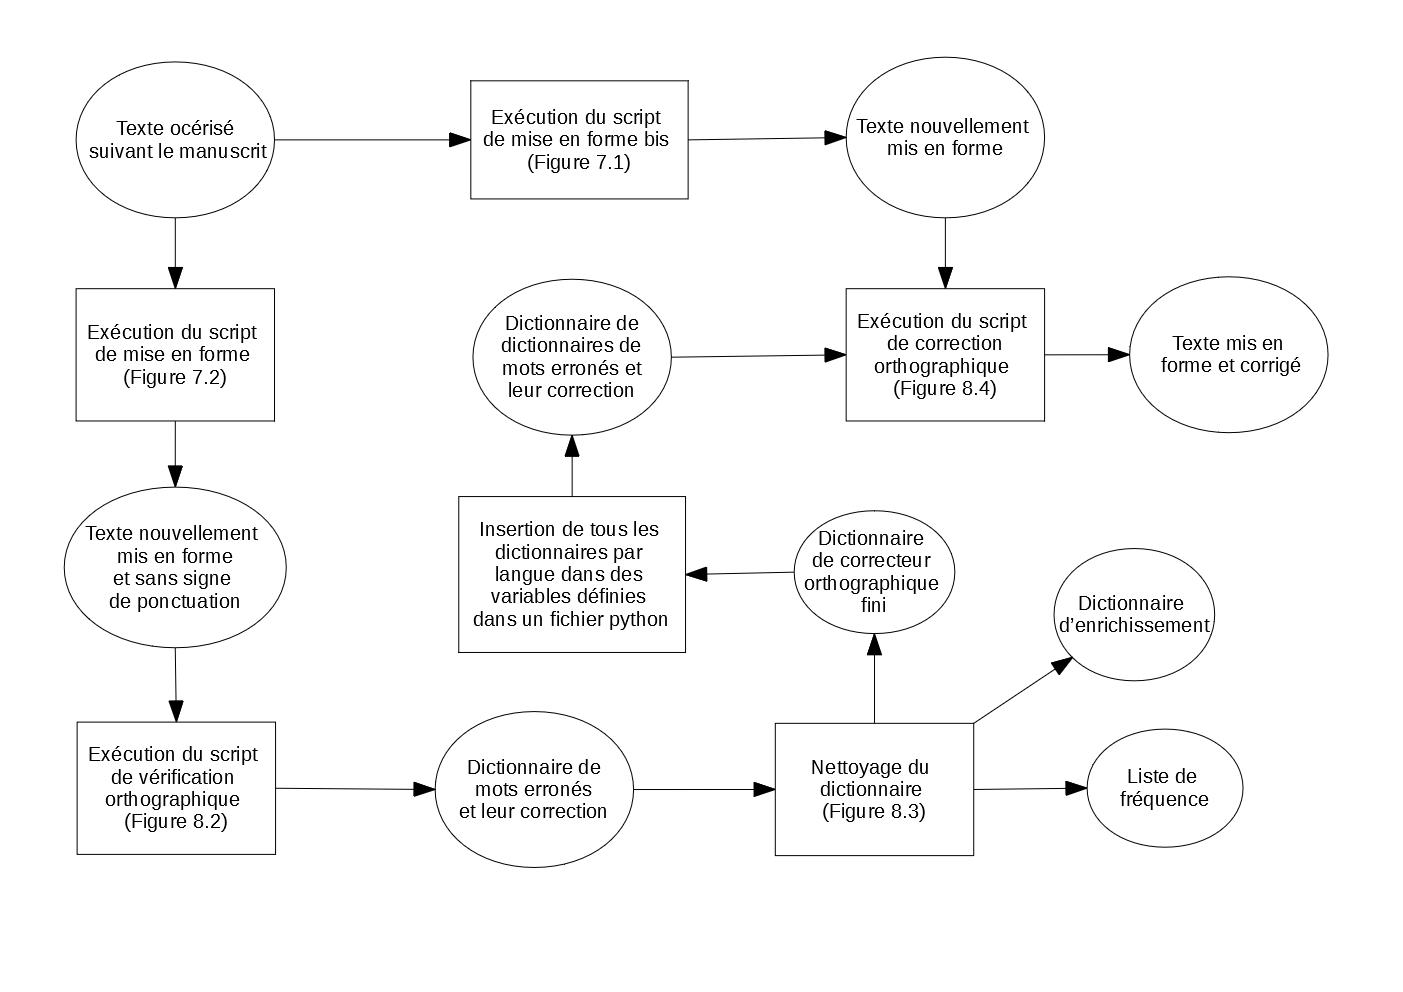
\includegraphics[width=16cm]{Partie2/schemas/Etapes_pour_la_finalisation.jpg}}
    \caption{Diagramme d'activité représentant les étapes pour atteindre une version finalisée et analysable du texte}
    \label{fig:etapestotales}
\end{figure}
Ce diagramme montre le processus qui permettra de partir du texte océrisé de la transcription exacte du manuscrit et d'obtenir une version uniformisée pour permettre une analyse textuelle. Le processus ira tout d'abord changer la mise en forme du texte, pour obtenir une version standard, en supprimant également la ponctuation pour donner la possibilité de traiter le texte et de relever les erreurs orthographiques. Ces erreurs seront traités de trois manières~: soit elles seront inscrites dans une liste pour être plus tard ajoutées aux dictionnaires de langue, soit elles seront inscrites dans un dictionnaire pour recenser les versions non usuelles du mot, soit elles seront ajoutées dans un dictionnaire de correcteur orthographique qui sera manipulé en même temps que le texte. Le dictionnaire orthographique contiendra les mots erronés et leur correction et il sera appliqué, à l'aide d'un autre traitement, au texte de base mis en forme mais cette fois-ci avec sa ponctuation, pour obtenir une version finalisée propre, sans erreur orthographique et prête à être analysée.

\subsection{Une première mise en forme du texte pour faciliter le correcteur}
La première étape consiste à appliquer le script de mise en forme créé précédemment (voir figure \ref{fig:etape1}), pour que le module orthographique puisse plus facilement trouver les mots erronés, sans de multiples tirets ou sans des caractères qui pourraient présenter un problème aux modules. Dans ce cas, nous allons également un peu plus loin que le script de mise en forme basique et nous lui faisons supprimer tous les signes de ponctuation. En effet, ces caractères ont tendance à gêner le correcteur, comme l'apostrophe, puisque le correcteur considère un déterminant et un nom rattaché par une apostrophe comme un mot et de ce point de vue, il ne peut pas le reconnaître, d'où l'intérêt de supprimer ces signes. Pour le cas des points, c'est également nécessaire de les supprimer car lorsqu'une phrase est finie et qu'un point est donc apposé à un mot pour marquer la fin, le correcteur considère le mot avec le point comme une entité et cela l'empêche à nouveau de reconnaître ce qu'il a devant lui. Nous avons donc décidé que pour plus de clarté, il faut supprimer ces éléments-là avant de mettre en fonction le correcteur et de faciliter son application.

\subsection{Éditer le dictionnaire de mots~: trouver les erreurs dans le texte}
La deuxième étape consiste à mettre en application le script de vérification orthographique, pour aller chercher les erreurs du texte pour effectuer plus tard leur correction.
\begin{figure}[t]
    \centering
    \caption{Diagramme d'activité représentant le fonctionnement de la vérification orthographique}
    \fbox{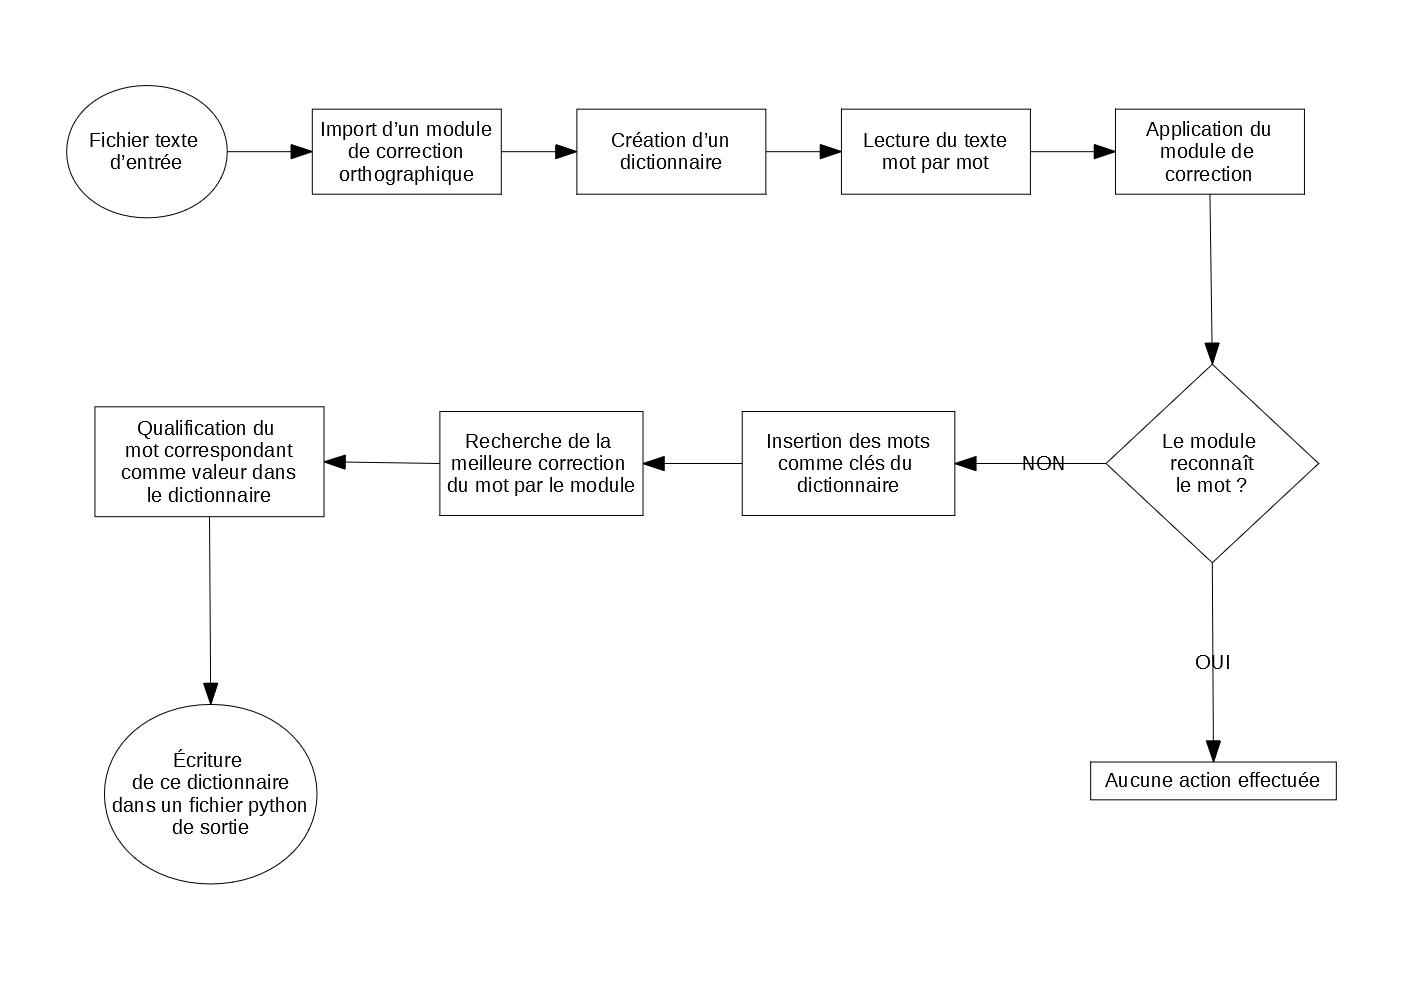
\includegraphics[width=14cm]{Partie2/schemas/2_module_orthographique.jpg}}
    \label{fig:etape2}
\end{figure}
Le processus se déroule comme montré dans la figure \ref{fig:etape2}~: à l'aide d'un module de correction orthographique, un fichier texte sera lu et le module cherchera s'il connaît ou non le mot. Lorsqu'il ne le reconnaîtra pas, ce mot sera inséré dans un fichier extérieur et le module cherchera sa correction la plus probable et lui assignera, créant ainsi un fichier de dictionnaire de mots, utilisable ultérieurement.

En effet, ce script aura pour but de créer un dictionnaire de mots que nous utiliserons ensuite pour corriger le texte mis en forme. Il est établi à l'aide d'une boucle \textit{for} et il consiste à aller chercher dans le texte les mots que le dictionnaire de fréquences de mots ne reconnaît pas. À partir de là, ces mots sont transformés en clés pour le dictionnaire et la valeur de chacune de ces clés est définie comme étant la correction la plus appropriée que conseille le module \emph{pyspellchecker}. Nous obtenons alors un dictionnaire dans un fichier Python qui correspondra à ceci~: \mint{python}{dico = {"mot erroné": "correction proposée"}}

\subsection{Une seconde mise en forme du texte pour rétablir certains éléments}
Une fois la manipulation faite avec le module, le script de mise en forme est de nouveau appliqué, cette fois-ci sans la fonction \og~supprimer\_ponctuation~\fg{}, puisque l'objectif maintenant sera d'avoir un fichier valide, lisible et cohérent et ces éléments-là en sont essentiels (voir figure \ref{fig:etape3}). L'extraction des mots erronés étant faite, nous pouvons récupérer le texte comme nous souhaitions le voir dans le cadre de la réelle mise en forme.

\subsection{Travail sur trois tâches en simultané}
La quatrième étape est probablement la plus rigoureuse de toutes, puisque nous devrons effectuer des changements à la main et au plus proche du texte, pour rendre le travail du correcteur orthographique le plus parfait possible et avoir finalement un document prêt pour une analyse approfondie. Cette étape consiste à la correction du dictionnaire de mots créé deux étapes plus tôt. Nous observons les mots et corrections proposées dans le dictionnaire, pour effectuer quelques modifications si nécessaires pour une correction efficace et cela mène à la réalisation de trois tâches autres mais liées entre elles.
\begin{figure}[H]
    \centering
    \fbox{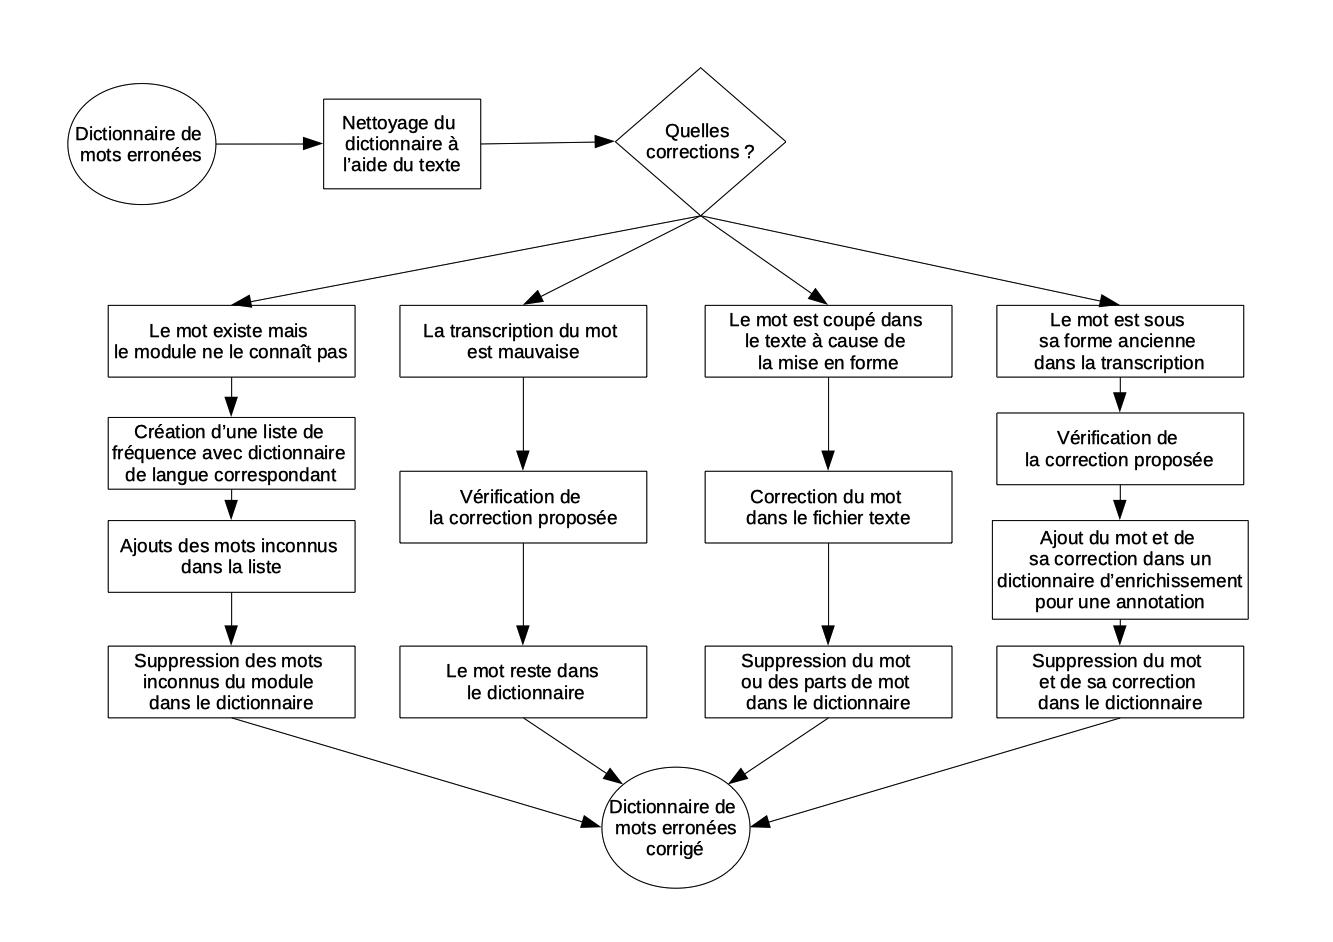
\includegraphics[width=15cm]{Partie2/schemas/4_nettoyage_dico.jpg}}
    \caption{Diagramme d'activité montrant les différentes actions qui permettent le nettoyage du dictionnaire de mots}
    \label{fig:etape4}
\end{figure}
Le dictionnaire de mots erronés nécessite un nettoyage qui s'effectuera à l'aide de quatre actions différentes~: soit le mot existe mais n'est pas connu par le module et il est ajouté à l'aide d'une liste de fréquence, soit le mot est mal transcrit dans le texte et sa correction est laissée ainsi dans le dictionnaire, soit la nouvelle mise en forme du texte a créé des erreurs dans l'écriture du mot et cela est corrigé à même le texte, soit le mot est sous une forme ancienne et il est ajouté dans un dictionnaire d'enrichissement. Une fois cela fait, le résultat est un dictionnaire de mots erronés et leur correction applicable au texte.

\subsubsection{Créer et développer la liste de fréquences}
Tout d'abord, nous observons les mots proposés comme erronés dans le texte par le correcteur orthographique et il arrive à plusieurs reprises que le mot existe et correspond exactement à ce que voulait dire l'auteur mais que le module Python ne le connaisse pas. Dans ce cas-là, ces mots sont supprimés du dictionnaire puisqu'ils doivent être conservés ainsi dans le texte. Ils sont ensuite intégrés dans un script Python qui contiendra une liste de mots qui seront ajoutés dans le dictionnaire de fréquences en fonction de la langue sélectionnée. Cela peut concerner des mots qu'il ne connaît pas, des versions plurielles et féminines du mot ou des conjugaisons qui lui sont inconnues.

\subsubsection{Opérer des changements directs dans le fichier texte}
Si le correcteur trouve des mots qu'il ne connaît pas et qui lui sont rajoutés avec la liste de fréquences, il trouve aussi parfois des erreurs qui vont nécessiter de corriger directement le texte, car cela ne serait pas pratique de le faire avec le script de correction orthographique. Ces modifications expliquent que la deuxième mise en forme se fasse à l'étape précédente, puisqu'il est nécessaire que le texte soit correctement présenté pour ensuite y faire des modifications.

Ainsi, il arrive que des erreurs apparaissent, notamment dues à la séparation par tirets qui existait dans la version originale de la transcription. Le script de mise en forme n'a pas complètement rattaché le mot, ce qui apparaît comme une erreur, que nous corrigerons directement dans le texte, plutôt que de laisser le correcteur le faire. Il faut aussi à l'inverse remettre parfois des tirets, lorsque le mot était composé mais qu'il avait été séparé à une fin de ligne. Ce sont des changements mineurs de vérification du texte transformé mais qui permettent un traitement exhaustif du document.

\subsubsection{Créer un dictionnaire d'enrichissement}
Nos textes de Beccaria ont été édités environ entre 1760 et 1800. A l'époque donc, pour certaines des langues, l'écriture se faisait dans ce qui s'appelle aujourd'hui une langue désuète (ancien français ou autre) avec des versions de certains mots (noms, verbes et leurs conjugaisons) qui ne sont pas les mêmes qu'aujourd'hui. Si nous avons décidé de conserver cela pour nos analyses de texte, il est cependant nécessaire de relever ces mots. Le module le fera logiquement puisque ces formes n'existent pas dans sa base de données. Nous les extrairons à notre tour du dictionnaire de correction et les insérerons dans un dictionnaire d'enrichissement qui servira par la suite à ajouter ces mots à nos modules d'analyses textuelles et notamment \textsc{txm}, pour qu'ils reconnaissent la forme lorsqu'il étudie nos textes.

\subsection{Application du dictionnaire de corrections sur le texte pour obtenir une version finalisée}
Après le travail sur le texte et sur le dictionnaire terminé, nous pouvons passer à la dernière étape, c'est-à-dire apporter les corrections insérées dans le dictionnaire au fichier texte, à l'aide d'un autre script Python.  Après avoir fait les dictionnaires pour chacune des éditions du Beccaria dans une même langue, ils sont tous placés dans un même fichier Python avec une variable donnée à chaque fois (généralement le nom de l'édition auquel il appartient en respectant le sigle défini). Ce fichier de dictionnaires sera par la suite appelé dans le script Python qui est utilisé pour la correction, à l'aide d'une variable.
\begin{figure}[H]
    \centering
    \fbox{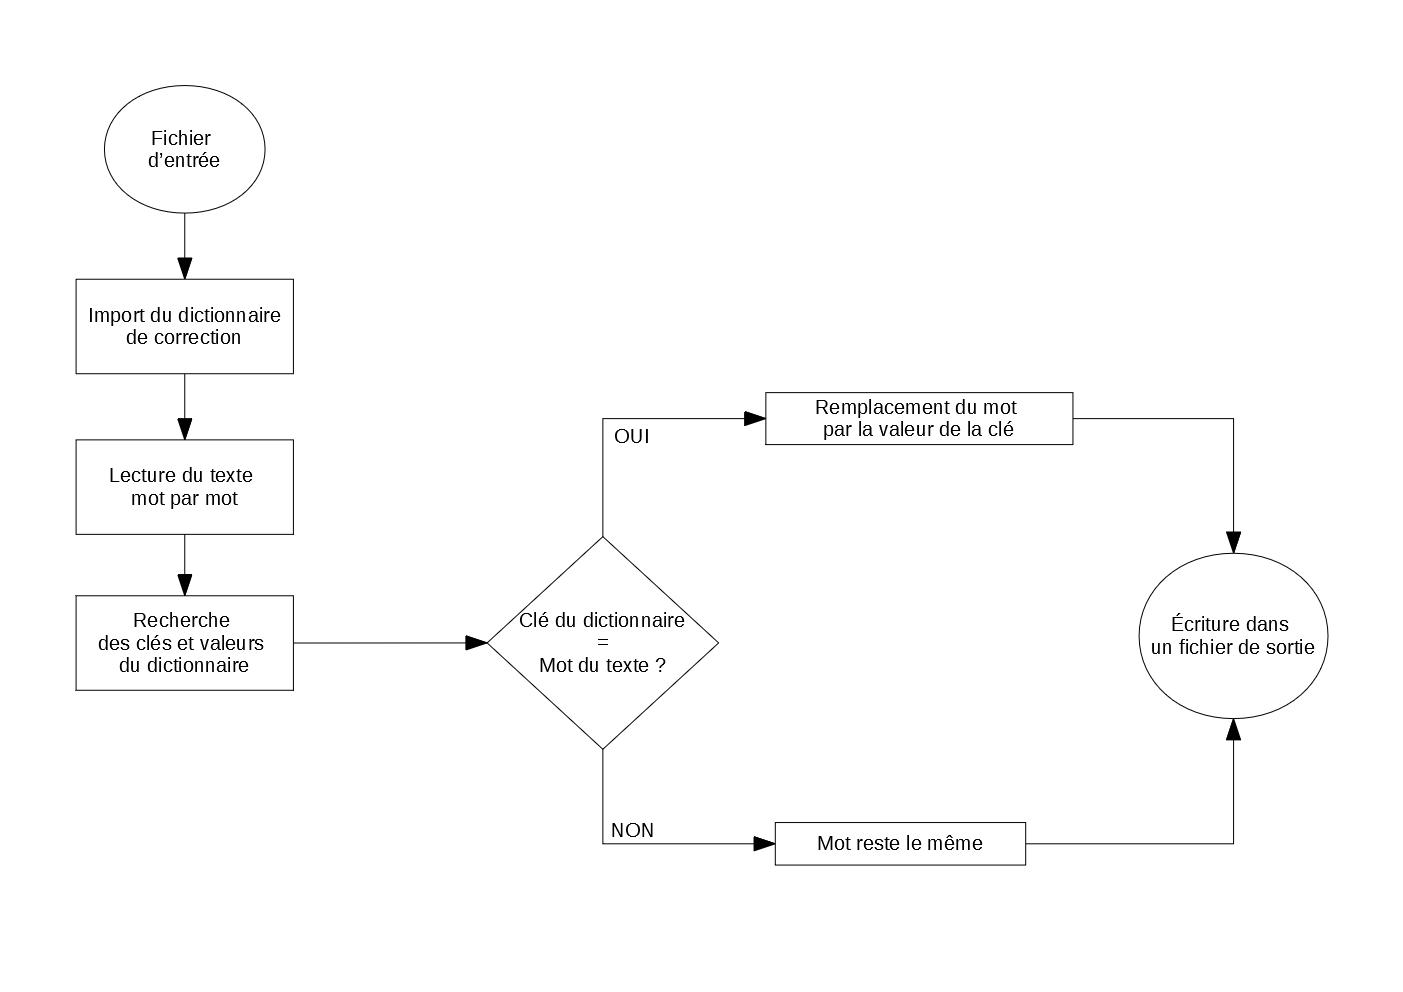
\includegraphics[width=15cm]{Partie2/schemas/5_correction.jpg}}
    \caption{Diagramme d'activité présentant la méthode d'application des corrections orthographiques}
    \label{fig:etape5}
\end{figure}
Le processus consistera à appeler le dictionnaire de mots qui a été traité précédemment et de faire chercher dans le texte les mots qui le composent. Si un mot correspond à un trouvé dans le dictionnaire, le traitement consistera à échanger ce mot par la valeur trouvée dans le dictionnaire, obtenant ainsi une version correcte et propre du texte.

\paragraph{} Le script Python correspondant consiste en une boucle \textit{for} qui sera liée au texte donné et au dictionnaire mis en variable. Il se base sur les clés et les valeurs de ce dictionnaire et il doit simplement aller lire le texte mot à mot, et dans le cas où il trouve un des mots qui font partis des clés de dictionnaires (\mintinline[breaklines]{python}{if cle in texte:}), il doit remplacer ce mot par la valeur de la clé dans le dictionnaire (\mintinline[breaklines]{python}{texte = texte.replace(cle, valeur)}). Ainsi, tous les mots relevés erronés dans le texte seront corrigés et nous obtenons un fichier texte correct orthographiquement, pratique pour l'analyse qui suivra.

\section{Les améliorations à apporter sur le module de correcteur orthographique}
Les différents scripts Python créés fonctionnent aussi bien que souhaité et ils s'adaptent bien au travail que doit réaliser le module \emph{pyspellchecker} mais il est tout de même possible de souligner certains changements à appliquer à l'un ou à l'autre pour une plus grande efficacité dans la correction et pour une meilleure utilisation.

\subsection{Apporter des éléments aux dictionnaires présents~: les listes de fréquences}
Le dictionnaire de mots qui est fourni dans le module de vérificateur orthographique n'est pas exhaustif, comme cela s'observe dans la figure \ref{fig:etape4}, puisqu'il lui arrive d'indiquer certains mots du texte comme faux, alors que ce n'est pas le cas. Lorsque ces cas se présentent, nous mettons en place une liste de fréquence (présente pour chacune des langues travaillées), ce qui fait partie des options proposées par le module \emph{pyspellchecker}.

En effet, dans un souci d'amélioration constante du module et d'application à son propre travail, il est possible d'ajouter des informations dans les dictionnaires avec lesquels nous travaillons. Ainsi, nous pouvons soit mettre un texte entier où tous les mots seront lus et analysés pour être ajoutés ensuite dans le dictionnaire, soit proposer une liste de mots dans le dictionnaire (la méthode choisie), soit n'ajouter qu'un seul mot. Il est également possible d'en supprimer du dictionnaire par la suite.

Alors, en prenant en compte cela, nous avons décidé de créer une liste de fréquences pour chacune des langues, complétée par de nouveaux mots à chaque nouvelle édition d'un dictionnaire depuis un fichier texte et qui s'ajoute au dictionnaire de langue fourni par le module, à chaque fin de travail sur un chapitre particulier.

\subsection{Importer un nouveau dictionnaire de langue~: l'exemple de l'italien}
Pour notre travail sur le traité\index{Traite des delits et des peines@Traité des délits et des peines} de Beccaria, nous étudions des éditions en quatre langues distinctes, dont notamment l'italien, langue d'origine de l'auteur. Cependant, cela a posé problème avec notre module de vérificateur orthographique, puisque cela ne fait pas partie des langues à sa disposition. Il a donc fallu trouver un moyen d'obtenir l'italien pour pouvoir faire une correction de tous les textes à disposition et d'avoir ainsi tous les éléments nécessaires pour l'analyse qui viendra après.

Pour se faire, je suis allée chercher sur le Github qui contient toutes les informations à propos de \emph{pyspellchecker}. Les \emph{issues} du Github m'ont permis de trouver la solution à ce problème, puisque l'une des questions posées était sur l'ajout d'une nouvelle langue dans le module et les moyens utilisés pour le faire \footnote{How to add a new langage \#26~: \url{https://github.com/barrust/pyspellchecker/issues/26}}. L'\textit{issue} renvoie à un autre compte Github qui contient de nombreuses langues avec des listes de fréquences de mots \footnote{FrequencyWords~: \url{https://github.com/hermitdave/FrequencyWords}}, dont notamment l'italien \footnote{\url{https://github.com/hermitdave/FrequencyWords/tree/master/content/2018/it}}. Nous avons donc pu extraire cette liste de mots, la transformer en un dictionnaire de langue, à l'aide d'un script, où le mot correspond à la clé et la fréquence correspond à la valeur et effectuer quelques modifications pour que le fichier soit valide. Une fois cela fait, en suivant les étapes mentionnées dans l'\textit{issue}, nous avons pu insérer le dictionnaire dans le script de vérificateur orthographique utilisé selon la figure \ref{fig:etape2} et ainsi, corriger également les éditions italiennes.

\subsection{Mise en place de lignes de commandes pour l'application du correcteur orthographique}
Enfin, l'une des dernières améliorations concerne moins le module orthographique que son application, et notamment un moyen de simplifier cette application. Le procédé pour corriger le texte contient tout de même quatre à cinq étapes, réalisées pour quatre langues différentes et il est donc nécessaire d'automatiser un minimum ces actions pour gagner du temps et réaliser plus rapidement ces changements.

Nous mettons ainsi en place des scripts shell qui vont contenir les lignes de commande liées au différentes étapes, que nous n'aurons qu'à entrer dans le terminal pour qu'il effectue en une fois tous les changements voulus, tout en respectant cependant chacune des étapes. Ces scripts, identifiés par une extension \emph{.sh}, commencent tous par une ligne unique, essentiel pour définir le fichier comme un script shell, soit \og\#!/bin/bash~\fg{}. Ensuite, sont écrites les informations nécessaires à l'application de nos scripts. Les scripts des trois premières étapes sont très similaires, puisque le changement concerne principalement les chemins des fichiers d'entrées et de sorties et il y a sinon une ligne pour chacune des langues. La quatrième étape est manuelle et donc ne nécessite pas de script. Ce sera pour la cinquième et dernière étape que la création de ces fichiers est la plus nécessaire, puisque là où précédemment, une ligne de commande suffisait pour un dossier complet contenant tous les fichiers d'une même langue, cela n'est pas possible pour la dernière étape. Il est en effet essentiel de préciser pour chacune des éditions le nom du fichier d'entrée et de sortie mais surtout la variable que le script devra aller chercher dans le dictionnaire importé, pour corriger correctement nos documents. Cela équivaut à six à huit lignes de commande, en fonction du nombre d'éditions, ce qui prendrait beaucoup de place et de temps à faire individuellement dans le terminal. Il est donc nécessaire de créer un fichier de ligne de commande pour chacune des langues et de changer le script à chaque nouvelle langue pour appeler le dictionnaire.

Par conséquent, grâce à cette méthode, l'application de notre correcteur orthographique est simplifiée, ce qui permet de corriger plus rapidement et plus efficacement nos fichiers texte, permettant ainsi de procéder plus rapidement au véritable travail à effectuer sur ces éditions, à savoir l'analyse et l'alignement\index{Alignement} des textes.

\part{Vers un alignement de texte~: analyse et exploration de la source}
\fancyhead[LO, RE]{Vers un alignement de texte}
Après avoir finalisé la transcription et la correction des chapitres choisis, le corpus est prêt à être étudié pour aboutir finalement à l'alignement\index{Alignement} recherché dans le cadre du projet de stage. Il existe de nombreux moyens d'analyser un texte, en fonction de ce que l'on veut faire ressortir de notre examen et celui-ci utilisera plusieurs de ces techniques.

Dans notre cas précis, nous allons principalement faire une analyse statistique des données textuelles de la source. Au fur et à mesure des étapes et à l'aide de plusieurs outils spécifiques, nous interrogerons le texte, premièrement, de manière assez superficielle, puis en se plongeant plus en avant dans le texte et enfin atteindre notre objectif, l'alignement\index{Alignement}, qui ne sera ici qu'un alignement partiel\index{Alignement!alignement partiel}, qui tient compte d'un lexique de termes juridiques préalablement choisis et annotés dans le texte.

\chapter{Appréhender la source et se familiariser avec son contenu}
\fancyhead[LO, RE]{Appréhender la source}

Dans un premier temps, pour entreprendre l'analyse du texte, il est nécessaire de se familiariser complètement avec le corpus sur la forme et sur le fond, dans l'ensemble et en comptant les pages de titres, pour arriver à de premières conclusions, à explorer ensuite plus, par le biais de plusieurs manipulations. Ainsi, nous commençons par étudier, sur la forme, les différentes éditions de l'ouvrage de Beccaria et collectons divers types d'informations à propos des ouvrages, pour voir les différences entre les éditions, les similarités et autres détails qui pourraient importer pour la poursuite de l'étude des textes, avec nos outils de textométrie\index{Textometrie@Textométrie}. Pour réaliser ce travail, nous avons divisé la tâche en deux parties~: tout d'abord, une lecture et une étude approfondie des textes puis un travail basique de ces textes avec deux/trois outils de textométrie\index{Textometrie@Textométrie}.

\section{Prise de connaissance du corpus~: premières lectures et explorations des sources à disposition}
Après avoir lu l'ouvrage en son entier pour connaître complètement le corpus et pouvoir travailler plus facilement par la suite certains des chapitres en connaissance de cause, je me suis intéressée à lire attentivement tous les \textsc{pdf} et les transcriptions préparées pour le séminaire de février, documents qui représentent ma source de travail pour la majorité de la période du stage, sans l'océrisation\index{OCR!ocerisation@océrisation} de nouveaux chapitres. Cette source se compose donc de plusieurs fichiers en quatre langues (italien, français, anglais, allemand), avec entre cinq et huit documents par langue comprenant les pages de garde de chacune des éditions et l'entièreté du chapitre 30-31-36 dans sa version \textsc{pdf} puis dans la version transcrite. L'objectif était donc de lire chacune des versions pour répertorier les premières différences que je pourrais confirmer par la suite, à l'aide de divers outils.

Cette étude s'est faite principalement avec l'observation des \textsc{pdf} que j'avais à disposition \footnote{Lors de la réalisation de cette étude et la production des tableaux, figures, etc., tous les \textsc{pdf} à disposition, n'avaient pas encore été retrouvés. Il est donc possible qu'il manque certaines éditions, pourtant mentionnées dans d'autres chapitres du mémoire.} et j'ai consigné la plupart des détails relevés dans des tableaux pour avoir une vision globale des similitudes et différences entre versions d'une même langue. Tout d'abord, la première observation consistait à lire la page de garde pour voir si des détails se trouvaient dessus pour discerner des micro changements entre les éditions de même langue, outre la date et le lieu d'édition. De ce fait, nous observons notamment l'origine de l'édition lors d'une traduction et par ce moyen, remarquer par exemple si un ouvrage a été traduit directement depuis la version de Beccaria\index{Beccaria, marquis de} ou si les éditeurs se sont basés sur la version faite par Morellet\index{Morellet, Andre@Morellet, André}.
\begin{figure}[H]
    \centering
    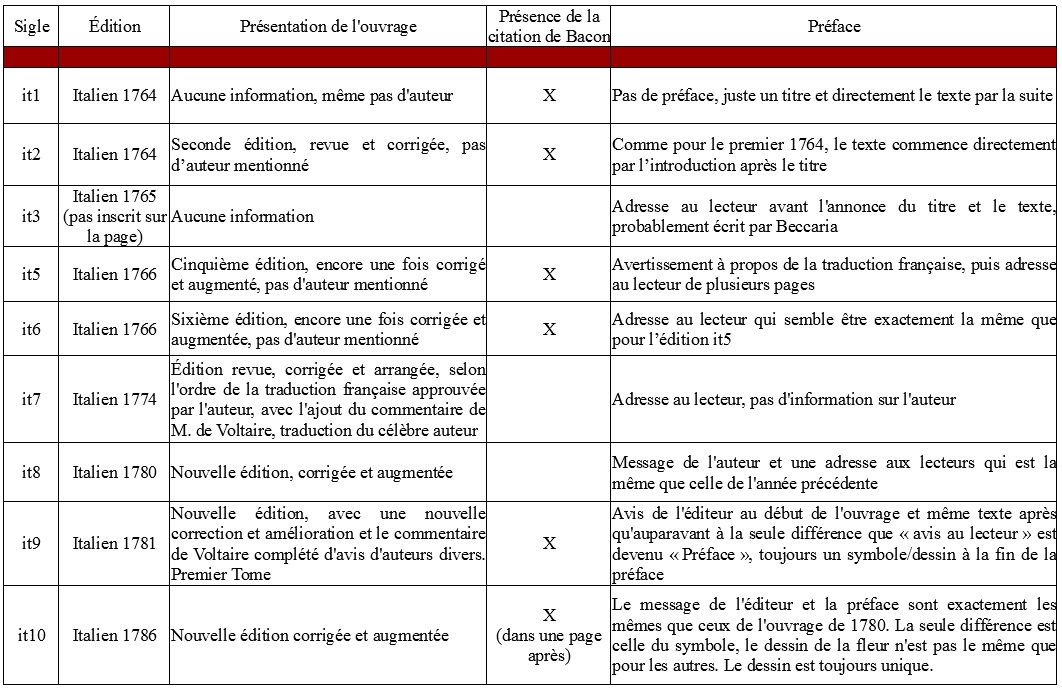
\includegraphics[width=16cm]{Partie3/images/chap1/Editions_it.jpg}
    \caption{Tableau d'observation réalisé pour les pages de garde et préfaces des éditions italiennes}
    \label{fig:editions_it}
\end{figure}
Ensuite, je me suis concentrée sur le contenu même du chapitre donné, pour voir comment le texte a été écrit, pour distinguer les différences d'écriture (si certaines lettres ne sont pas les mêmes qu'aujourd'hui, si les mots sont désuets, etc.), pour constater que certains des éditeurs avaient effectué des changements, que ce soit en insertion de notes de bas de page comme cela peut être le cas pour la majorité des éditions allemandes ou bien même si le texte a été particulièrement modifié dans sa structure comme c'est le cas avec les éditions produites en français en 1766(fr1-1) et 1797(fr1-2).
\begin{figure}[H]
    \centering
    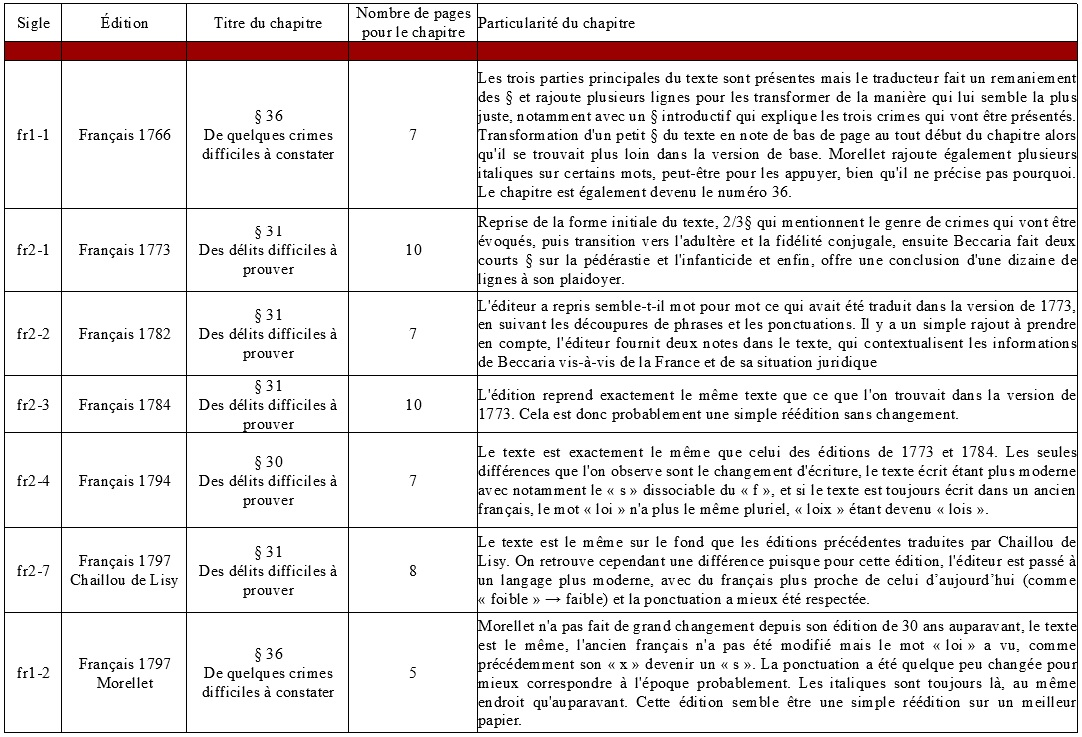
\includegraphics[width=16cm]{Partie3/images/chap1/Chaps_fr.jpg}
    \caption{Tableau d'observation réalisé pour le chapitre 30/31/36 des éditions françaises}
    \label{fig:editions_fr}
\end{figure}
Une fois ces observations faites, nous pouvons tirer de premières conclusions. Il est déjà possible de remarquer que Morellet\index{Morellet, Andre@Morellet, André} a réalisé de grands changements dans le chapitre 30/31, devenu 36 pour lui, et qu'il ne semble plus y avoir de grandes similarités sur la structure du texte et même sur la manière dont les idées sont présentées. Si, dans le fond, ce qui est dit est fondamentalement la même chose, les tournures de phrases ne sont plus les mêmes, l'ordre de présentation des éléments semble avoir changé et il parait donc qu'il n'y a plus le même texte. Ensuite, nous pouvons aussi distinguer les changements apportés par les versions allemandes, qui sont composées en grande majorité de notes de bas de page. Ces notes semblent différer en fonction des éditions, puisque parfois elles sont explicatives pour donner plus de détails à ce qui est présenté et d'autres fois, elles reprennent des morceaux de texte trouvés dans d'autres versions allemandes. Enfin, la dernière observation, essentielle dans la recherche car liée à notre objectif d'établir une généalogie des éditions, est qu'un certain nombre de ces textes sont des rééditions~: la version de 1797 de Morellet\index{Morellet, Andre@Morellet, André} est une réédition de l'ouvrage de 1766 avec quelques modernisations de l'écriture et de termes~; les éditions anglaises d'après 1767 semblent être à chaque fois des rééditions de cette première version~; la version italienne de 1786 est rééditée depuis la version de 1780~; enfin, en allemand, l'édition de 1786 apparaît comme une stricte réédition de la version de 1778. \pagebreak

Ainsi, à travers tout cet examen des textes à disposition, il est déjà possible de cerner une partie des textes et leurs spécificités qui pourront être approfondies postérieurement. Cela permet d'établir une base de connaissances sur les textes qu'il sera possible de développer, d'argumenter ou de modifier avec l'utilisation des outils d'analyse textuelle.

Cette base de connaissances permet néanmoins déjà de répondre à un des objectifs fixés pendant le stage, à savoir la généalogie des éditions et des traductions. En effet, les membres du projet, aidés par le travail réalisé par Philippe Audegean\footcite[p.~33-117]{beccaria_audegean_2009}, avaient déjà regroupé des informations à propos des éditions qui permettaient de se faire une première idée de cette généalogie (informations que nous pouvons retrouver dans les tableaux \ref{table:editions}) et les observations supplémentaires faites pendant cette lecture du texte donnent la possibilité de réaliser cette généalogie, en regroupant toutes les informations à dispositions.
\begin{figure}[H]
    \centering
    \fbox{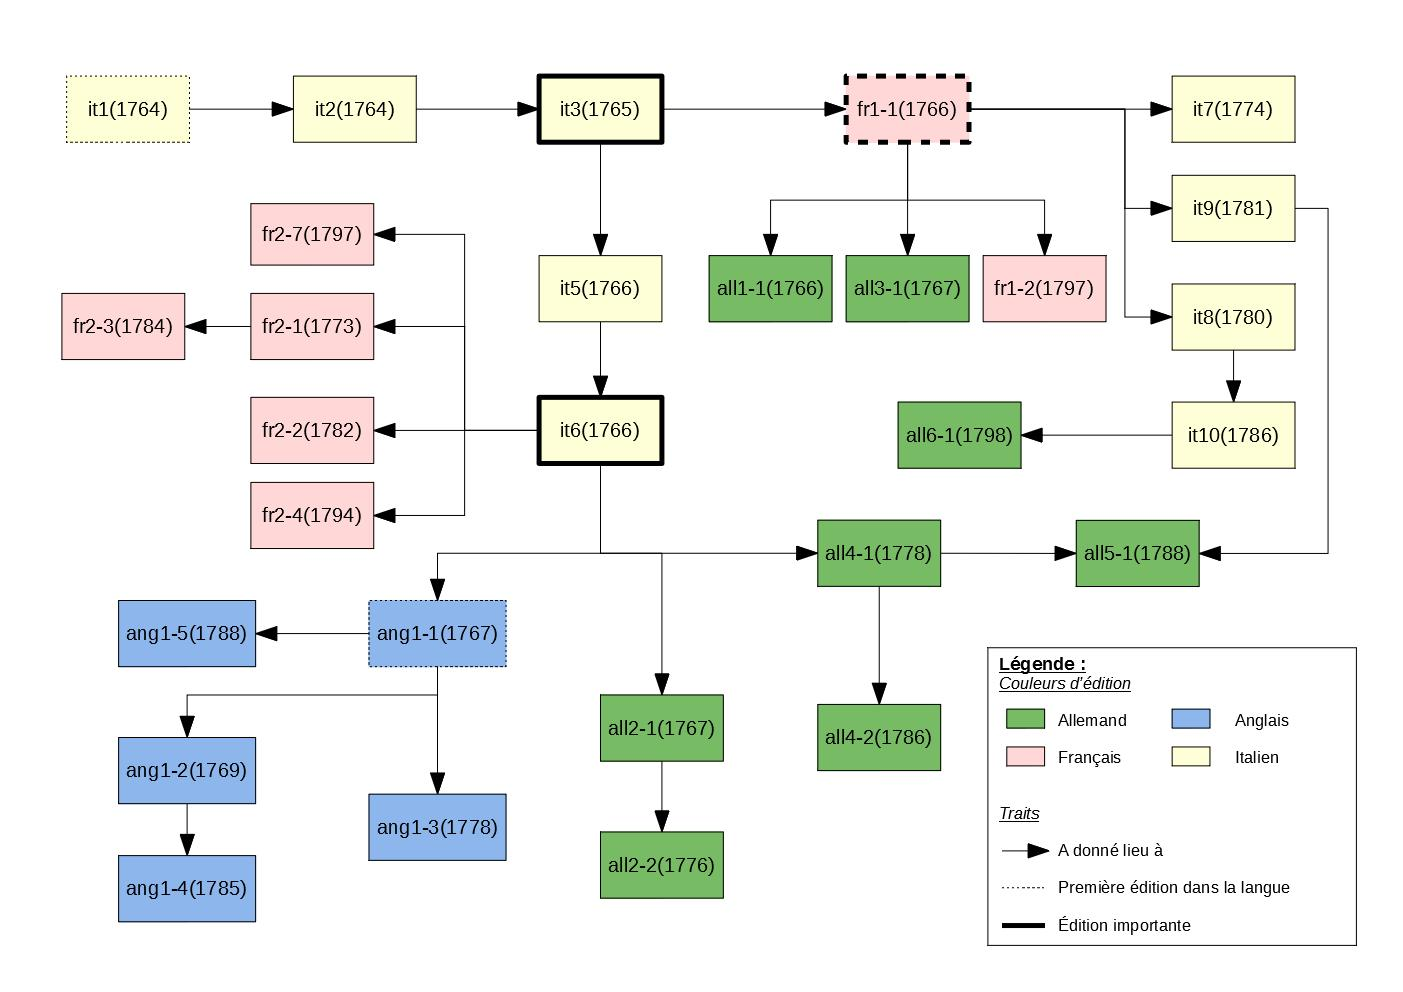
\includegraphics[width=15cm]{Partie3/images/chap1/genealogie.jpg}}
    \caption{Généalogie des éditions et traductions du \emph{Traité}\index{Traite des delits et des peines@Traité des délits et des peines} de Beccaria en italien, français, allemand et anglais}
    \label{fig:genealogie}
\end{figure}
À l'aide d'une lecture des titres de chaque édition du \emph{Traité}\index{Traite des delits et des peines@Traité des délits et des peines} de Beccaria à disposition et en feuilletant les premières pages de l'ouvrage pour observer la préface, les avis de lecteurs et les commentaires insérés, il est possible d'établir cette généalogie des éditions et traductions du texte pour pouvoir déterminer sur quel texte s'est basé chacun des éditeurs pour établir son édition. En l'état, il s'observe que l'abbé Morellet\index{Morellet, Andre@Morellet, André} est parti de la troisième édition de Beccaria\index{Beccaria, marquis de}, publié en 1765, pour effectuer ses modifications, donnant lieu ensuite à une autre publication française, deux allemandes et quatre publications italiennes. Deux de ces publications ont ensuite servies de base pour produire deux nouvelles éditions allemandes. Le texte a été édité cinq fois en italien avant d'arriver à la sixième édition, qui est le texte de départ pour les éditions anglaises, pour la majorité des textes français et pour deux éditions allemandes. Cette généalogie permet également de distinguer un certain nombre de rééditions d'une même langue, que cela soit le cas pour l'italien, le français, l'anglais ou l'allemand. Enfin, il y a un cas assez unique pour l'édition de  1788, qui se base sur l'édition italienne de 1781 pour son texte mais également sur l'édition allemande publiée en 1778, pour le cas de ses notes de bas de page.

\section{Examens préliminaires des textes de Beccaria~: découvrir les outils d'analyses textuelles}
Une fois les premières lectures effectuées, nous approfondissons notre recherche de base en utilisant quelques outils de textométrie\index{Textometrie@Textométrie} pour essayer de faire ressortir les caractéristiques observées précédemment, pour voir si nos premières conclusions se confirment, si une analyse sur le fond fait apparaître une vision contraire à celle que nous avons eue ou s'il n'y a que des différences légères. Pour réaliser cet examen, nous avons choisi trois outils~: un logiciel à télécharger, \textsc{txm}{\footcite{txm_plateforme}} et deux logiciels présents sur le web, \textsc{juxta commons}{\footnote{\url{http://juxtacommons.org/}}} et \textsc{medite}{\footnote{\url{http://obvil.lip6.fr/medite/}}}.

\subsection{Étudier les dimensions du corpus~: introduction à TXM}
\begin{figure}[t]
    \centering
    \caption{Production \textsc{txm} présentant les dimensions des corpus pour chaque langue par nombre de mots en fonction de chaque édition (haut gauche~: allemand, droit~: anglais, bas gauche~: français, droit~: italien)}
    \fbox{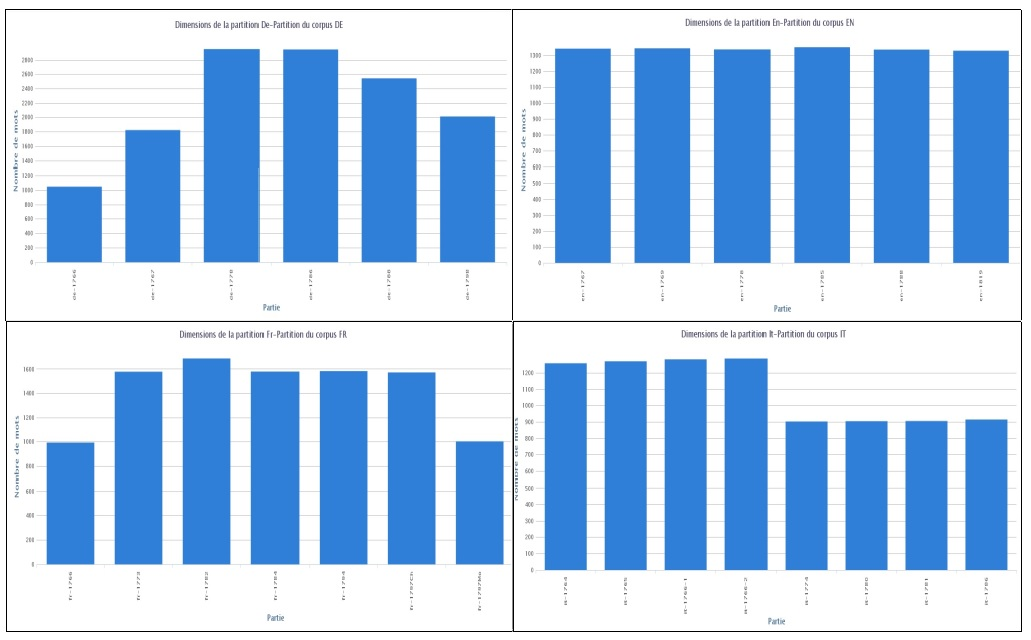
\includegraphics[width=14cm]{Partie3/images/chap1/Dimensions.jpg}}
    \label{fig:dimensions}
\end{figure}
Tout d'abord, nous pouvons vérifier certaines des conclusions à l'aide de \textsc{txm}, qui sera majoritairement utilisé pendant le stage. \textsc{txm} est un outil de textométrie\index{Textometrie@Textométrie} doté d'un certain nombre d'options permettant de faire apparaître divers types d'informations à propos d'un corpus. Parmi ces options, il y a \textbf{\textit{Propriétés}} qui s'applique au corpus ou à une version partitionnée \footnote{Apparition du corpus selon une unité structurelle différente (phrases, texte, etc.) et avec une propriété particulière (par langue, année, numéro de phrase, etc.)} et qui prend en compte le nombre de mots pour chacun des fichiers présents dans le corpus importé. À partir de cela, cet outil fait apparaître, sous forme d'un diagramme en barre, les dimensions du corpus (voir figure \ref{fig:dimensions}). Cette étape est très intéressante puisqu'elle permet de voir la diversité entre les langues et la différence ou non différence en fonction des éditions. Nous observons pour chacune des langues un trait caractéristique, qui va parfois dans le sens de ce qui a déjà été rapporté lors de la lecture du corpus, qui agrémente, d'autres fois, une précédente observation ou enfin, certaines qui nous font contempler des caractéristiques non observées auparavant. Ainsi, concurremment de ce qui avait été vu lors de la lecture du corpus, les éditions anglaises semblent effectivement être des rééditions strictes de la toute première parution, sans changement quel qu'il soit dans le cas du chapitre 31 au moins. Le corpus est constitué d'à peu près le même nombre de mots pour chacune des éditions, à quelques mots près, probablement dû à des erreurs d'\acrshort{ocr}\index{OCR} ou à des changements mineurs. Les autres corpus présentent des différences beaucoup plus flagrantes. Pour le cas de l'italien, il y a une démarcation claire entre les quatre premières éditions et les quatre dernières~: cela est dû à une différence de versions puisque les éditions de 1764, 1765 et les deux de 1766 sont ou reprennent le texte écrit par Beccaria\index{Beccaria, marquis de}, alors qu'à partir de 1774 et après en 1780, 1781 et 1786, la traduction italienne se fait depuis l'édition française créée par Morellet\index{Morellet, Andre@Morellet, André}, avec ses différentes modifications. Par cela s'observe donc le fait que la version de Morellet\index{Morellet, Andre@Morellet, André} supprime un certain nombre de mots dans le chapitre 30 de Beccaria\index{Beccaria, marquis de}, amenant à une traduction plus courte et bien différente, comme cela avait été observé avec la lecture du corpus italien et même français. Vis-à-vis des éditions françaises, nous distinguons également bien la démarcation entre la version de Morellet\index{Morellet, Andre@Morellet, André} et la version de Chaillou de Lisy\index{Chaillou de Lisy, Etienne}, qui traduit en suivant la structure de Beccaria\index{Beccaria, marquis de}. La différence dans le nombre de mots se discerne amplement et expose la divergence entre les deux. L'autre édition qui se détache un peu des autres est celle de 1782, qui semble dépasser d'une centaine de mots le reste des manuscrits non édités par Morellet\index{Morellet, Andre@Morellet, André}, ce qui est minime mais montre un écart. Cela est dû, d'après une recherche subséquente, à des notes de bas de pages intégrées dans cette version. Enfin, la dernière dimension de corpus est le cas de l'allemand qui présente le plus de dissimilitudes entre ses différentes versions. Ces variations semblent venir d'ajouts de notes de bas de pages, qui diffèrent en fonction de chaque version et de changements d'origine de la traduction (parfois Beccaria\index{Beccaria, marquis de}, parfois Morellet\index{Morellet, Andre@Morellet, André}). La seule observation qui confirme nos suppositions précédentes est le fait que la version de 1786 semble effectivement être une réédition de 1778, puisque l'outil atteste du même nombre de mots entre les deux.

Par cet outil, nous pouvons donc déjà contempler une certaine quantité de caractéristiques à propos du corpus, ce qui nous aide à mieux approfondir nos connaissances sur sa composition et sa structure, élément utile lorsqu'il sera étudié plus intérieurement.

\subsection{Comparer les textes entre eux~: manipulations avec Juxta Commons}
Nous pouvons ensuite passer à une étude plus portée sur le fond du texte et notamment sur les changements effectués dans les éditions au fur et à mesure des parutions. \textsc{juxta commons} est un outil parfait pour cela puisqu'une fois que le corpus lui est soumis, il le collationne et fait ensuite apparaître les textes sous différentes formes, telle que la \og~Heat Map~\fg{}, qui prend un texte de base et présente toutes les différences par rapport aux autres textes du corpus. La \og~Side-by-side view~\fg{}, autre option, sélectionne deux textes du corpus soumis et expose les différences entre les deux. Il y a aussi la \og~parallel-segmentation~\fg{} qui produit une édition critique en \textsc{xml} contenant tous les textes et des identifiants et témoins pour observer, selon un témoin de base, les endroits du texte où il y a une différence et comment celle-ci apparaît pour chacune des versions. Ces trois options sont les plus utiles pour faire ressortir les informations voulues. En majorité, l'utilisation de \textsc{juxta commons} a permis de faire ressortir ce qui avaient déjà été observés lors des premières explorations. La \og~parallel-segmentation~\fg{} est un outil parfaitement adapté pour les éditions anglaises puisque, comme nous le voyons, il n'y a que très peu de balises <rdg> (balises servant à faire ressortir les différences)~; généralement, ces différences sont dues à des erreurs d'\acrshort{ocr}\index{OCR} qui ont rendu un des mots incorrects dans une des versions. Cet outil démontre donc que l'anglais n'a que très peu de changements entre ses éditions. Le français et l'italien font très vite apparaître de grandes différences entre les versions mais cela est minimisé dès que sont créés des sous-corpus en fonction de l'origine des traductions~: d'un côté, les éditions avec la structure de Beccaria\index{Beccaria, marquis de} et de l'autre, les éditions avec celle de Morellet\index{Morellet, Andre@Morellet, André}. Une fois cela exécuté, nous ne remarquons que très peu de différences, à part des changements d'écriture avec des apparitions d'accents sur les mots pour l'italien et des modernisations de mots pour les deux langues. Enfin, les éditions allemandes sont peu adaptées à la \og~parallel-segmentation~\fg{} car les différences sont beaucoup trop importantes, de même pour la \og~side-by-side view~\fg{} qui montrera d'énormes changements entre les deux versions. Cela ne nous apporte qu'une confirmation de ce que nous avions conclu, à savoir que les éditions sont fondamentalement différentes, sauf, encore une fois, 1778 et 1786. Toutes ces considérations peuvent s'observer avec une des vues de la \og~Heat Map~\fg{} prenant l'édition de 1778 comme édition de base, qui montre que les différences entre les autres textes sont immenses et qu'il y en a même dans le cas de la réédition de 1786.
\begin{figure}[H]
    \centering
    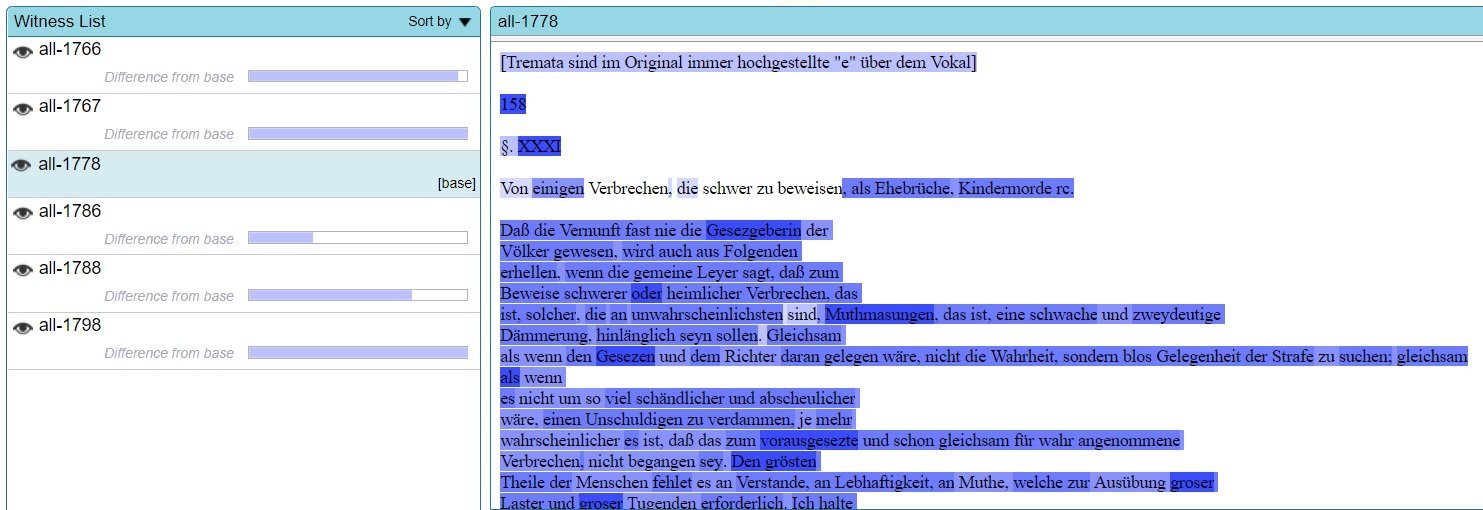
\includegraphics[width=16cm]{Partie3/images/chap1/Heat_Map.jpg}
    \caption{Démonstration des différences entre les éditions allemandes avec 1778 comme édition de base par la \og~Heat Map~\fg{} produite par \textsc{juxta commons}}
    \label{fig:heat_map}
\end{figure}
Ainsi, \textsc{juxta commons} est un outil pratique pour nos premières recherches puisqu'il confirme ce qui avait été supposé sur notre texte, les différences en fonction des langues, les similarités pour certaines des éditions et il est possible de discerner un semblant de schéma. Les éditions anglaises et allemandes sont à des opposés~: les premières ont un corpus quasi-identique alors que les secondes ont des caractéristiques particulières pour chacune des éditions. Au centre de ce schéma, se trouvent les corpus italiens et français qui ne diffèrent globalement qu'en fonction de l'origine des traductions.

\subsection{Confirmer ou non les observations précédentes~: l'analyse par MEDITE}
Pour finir notre travail préliminaire, un troisième outil d'analyse de texte est utilisé~: \textsc{medite}, un logiciel d'alignement\index{Alignement} de textes développé par le laboratoire d'excellence de l'\acrfull{obvil}. Il permet d'observer les suppressions, insertions, remplacements et déplacements entre deux textes et est donc une bonne base pour notre travail qui sera également un alignement\index{Alignement} de textes, mais il ne permet pas de réaliser un alignement multilingue\index{Alignement!alignement multilingue}, notre objectif. \textsc{medite} est assez similaire à la \og~side-by-side view~\fg{} de \textsc{juxta commons} mais le logiciel donne la possibilité de choisir des options d'affichage tel qu'une sensibilité à la casse ou une option pour qu'il ne fasse apparaître que les blocs en commun. Une fois les textes chargés, nous pouvons alors observer les variations avec des précisions indiquées sur le côté des textes, comme le montre la figure \ref{fig:medite}.
\begin{figure}[H]
    \centering
    \fbox{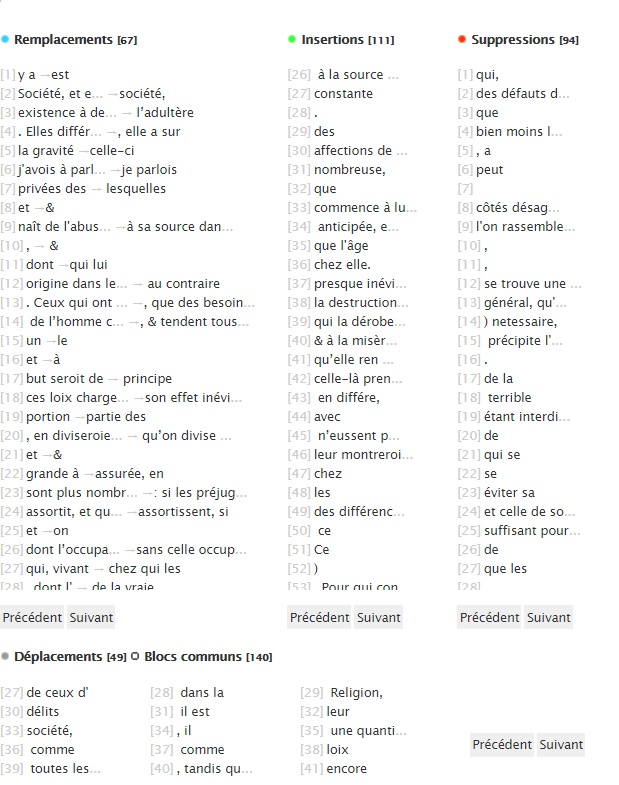
\includegraphics[width=15cm]{Partie3/images/chap1/MEDITE_alignement.jpg}}
    \caption{Alignement\index{Alignement} de textes~: présentation des remplacements, insertions, suppressions, déplacements et blocs communs entre le chapitre 30/31/36 des éditions françaises de 1766 et 1773}
    \label{fig:medite}
\end{figure}
L'outil est assez complet puisque nous pouvons observer les numéros de lignes où apparaissent ces changements, les différences quand il s'agit de remplacements et même le nombre de ces changements pour chaque catégorie.

Ce logiciel est bien adapté puisqu'il permet de vérifier les conclusions faites lors des examens précédents du texte. Nous pouvons ainsi choisir deux textes qui présentent ou non des altérités pour chacune des langues et alors constater si nos suppositions s'avèrent vraies. L'analyse suivante nous montre que cela n'est pas exactement le cas et que les textes ne sont pas toujours si différents que présumés.
\begin{figure}[H]
    \centering
    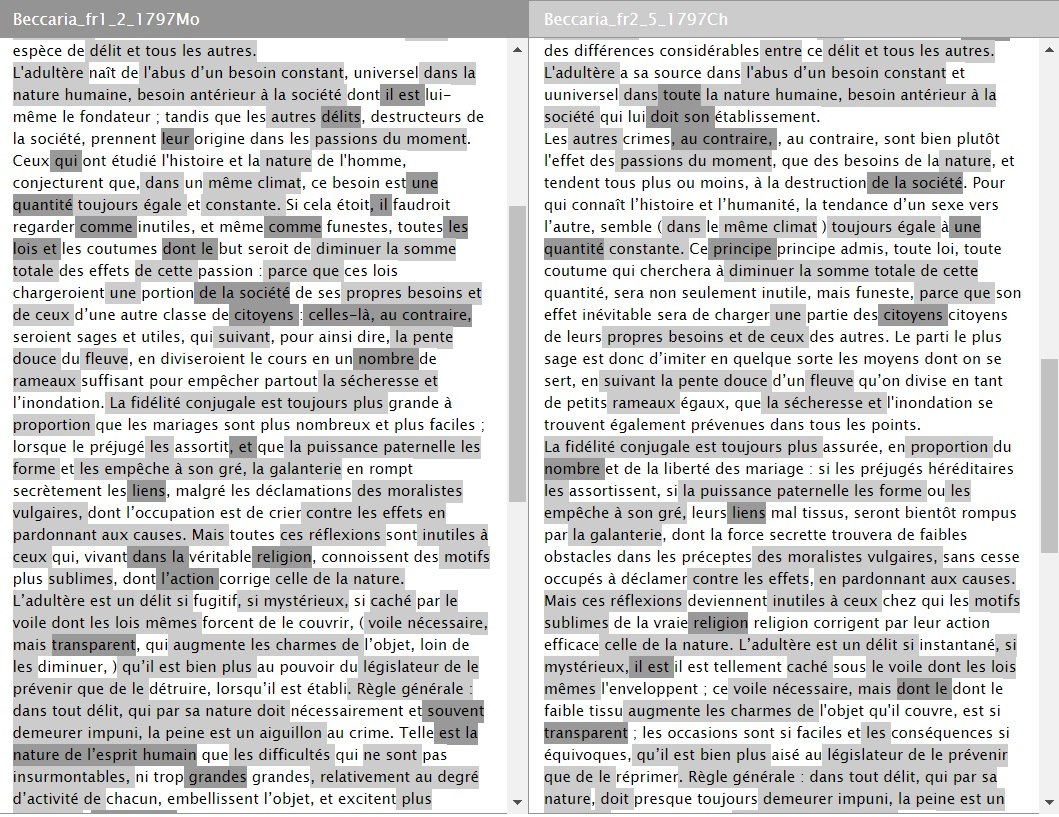
\includegraphics[width=15cm]{Partie3/images/chap1/MEDITE_fr.jpg}
    \caption{Alignement\index{Alignement} de textes entre l'édition française de 1797 de Morellet\index{Morellet, Andre@Morellet, André} et celle de 1797 de Chaillou\index{Chaillou de Lisy, Etienne}}
    \label{fig:medite_fr}
\end{figure}
En décidant de ne faire apparaître que les blocs communs entre une édition reprenant la structure de Morellet\index{Morellet, Andre@Morellet, André} et une reprenant celle de Beccaria\index{Beccaria, marquis de}, nous pouvons voir que les changements effectués par Morellet\index{Morellet, Andre@Morellet, André} ne sont pas si conséquents. Il semble avoir opérer un certain nombre de déplacements de paragraphes ou de groupes de mots, pour présenter le texte selon ce qu'il pensait être le mieux mais ces groupes de mots restent cependant les mêmes que ceux traduits depuis l'édition de Beccaria\index{Beccaria, marquis de}. Nous pouvons, de plus, confirmer ces observations avec le tableau \ref{table:alignement_medite_fr}, où nous avons fait une comparaison cette fois entre la première édition de Morellet\index{Morellet, Andre@Morellet, André} en 1766 et la première reprenant la structure de Beccaria\index{Beccaria, marquis de}. Nous pouvons voir qu'il y a eu un certain nombre de changements dont notamment des suppressions et quelques déplacements, mais le tableau montre tout de même une quantité de blocs communs (130). Le résultat du logiciel ne démonte pas complètement la théorie avancée, puisque les deux types d'éditions présentent effectivement un certain nombre de variations, même dans le cas des paragraphes où les idées sont les mêmes. La différence majeure est la suppression de deux paragraphes d'explications qu'avait inséré Beccaria\index{Beccaria, marquis de} au début du chapitre et qui ont été supprimés par Morellet\index{Morellet, Andre@Morellet, André}, ce qui s'observe ici par le biais de la barre de défilement qui est plus courte pour la version de Morellet\index{Morellet, Andre@Morellet, André}. Cela démontre un texte plus court que la version 1797 de Chaillou\index{Chaillou de Lisy, Etienne}. André Morellet\index{Morellet, Andre@Morellet, André}, dans sa traduction, semble avoir ensuite reformulé les idées, pour être plus direct dans son approche et exposer plus rapidement ses idées. Le tableau \ref{table:alignement_medite_fr} présente également, avec sa troisième et quatrième colonne, le fait que Morellet\index{Morellet, Andre@Morellet, André} a bien effectué une réédition en 1797, mais qu'il n'a pas changé beaucoup d'éléments, comme le montre les chiffres du tableau, notamment lorsque les séparateurs ne sont pas pris en compte. 

\begin{table}[H]
\centering
\begin{tabular}{|c|c|c|c|c|}
\hline
 & 1766 vs 1773 & 1766 vs 1773 & 1766 vs 1797Mo & 1766 vs 1797Mo \\
 & (avec s.) & (sans s.) & (avec s.) & (sans s.) \\ \hline
Remplacements & 67 & 62 & 53 & 52 \\ \hline
Insertions & 111 & 95 & 15 & 1 \\ \hline
Suppressions & 94 & 78 & 7 & 0 \\ \hline
Déplacements & 49 & 40 & 0 & 0 \\ \hline
Blocs Communs & 140 & 130 & 72 & 54 \\ \hline
\end{tabular}
\caption{Données de l'alignement entre les éditions françaises de 1766 et 1773 et 1766 et 1797 (Morellet), avec le comptage des séparateurs (!,;.?...) et sans}
\label{table:alignement_medite_fr}
\end{table}

C'est avec l'étude des versions italiennes que l'impact de \textsc{medite} est beaucoup plus important et significatif pour nos suppositions antérieures, comme le tableau \ref{table:alignement_medite_it} et la figure \ref{fig:medite_it} nous permettent de l'observer.
\begin{table}[H]
\centering
\begin{tabular}{|c|c|c|}
\hline
 & 1766 vs 1774 (avec s.) & 1766 vs 1774 (sans s.) \\ \hline
Remplacements & 53 & 36 \\ \hline
Insertions & 46 & 3 \\ \hline
Suppressions & 68 & 4 \\ \hline
Déplacements & 0 & 0 \\ \hline
Blocs Communs & 164 & 41 \\ \hline
\end{tabular}
\caption{Données de l'alignement entre les éditions italiennes de 1766 et 1774, avec le comptage des séparateurs (!,;.?...) et sans}
\label{table:alignement_medite_it}
\end{table}

\begin{figure}[H]
    \centering
    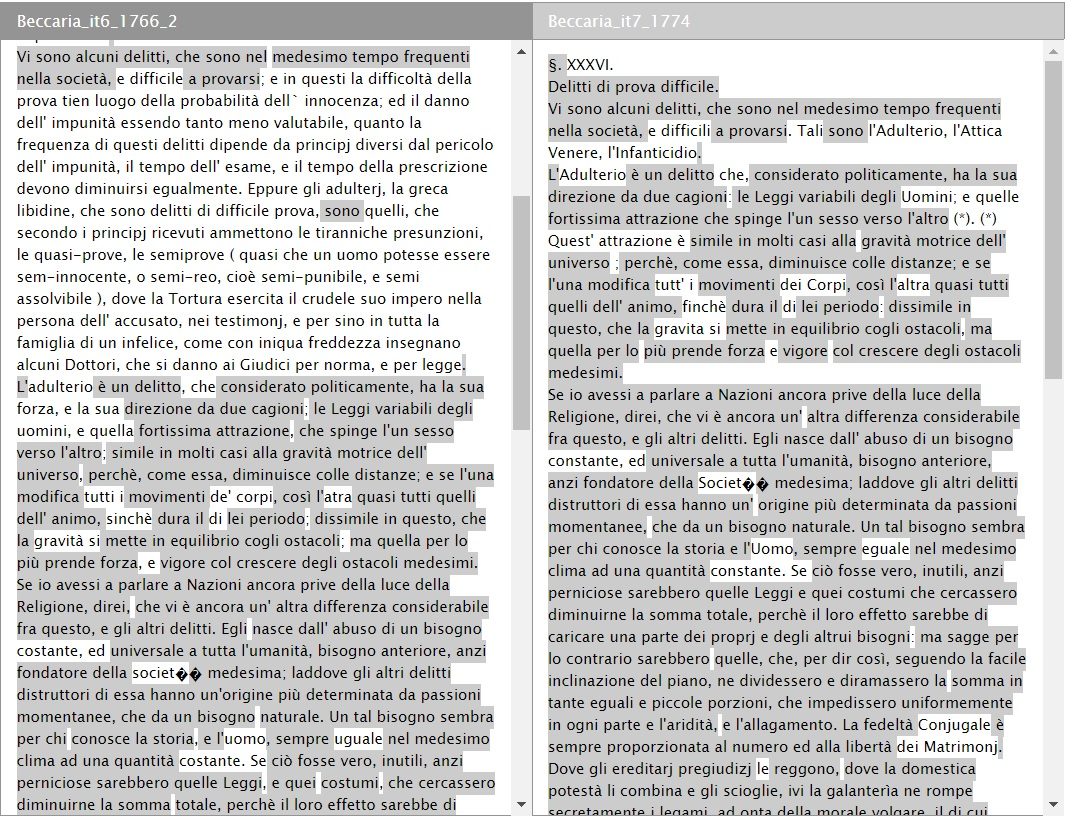
\includegraphics[width=15cm]{Partie3/images/chap1/MEDITE_it.jpg}
    \caption{Alignement\index{Alignement} de textes entre les éditions italiennes de 1766 et 1774}
    \label{fig:medite_it}
\end{figure}

L'édition de 1766 suit ce qui avait été écrit par Beccaria\index{Beccaria, marquis de} alors qu'à partir de l'édition de 1774, le \emph{Traité}\index{Traite des delits et des peines@Traité des délits et des peines} suit les changements effectués par Morellet\index{Morellet, Andre@Morellet, André}, avec une traduction italienne de la traduction française. Par le biais de ces colorations de blocs en commun, il est possible de voir que les deux versions italiennes ne sont pas aussi éloignées que nous le présumions. Il y a toujours le cas de ces deux premiers paragraphes de présentation que Morellet\index{Morellet, Andre@Morellet, André} a réduit, ce qui se matérialise probablement par la suppression de quatre blocs dans le tableau \ref{table:alignement_medite_it} mais outre cela, il y a de très grandes similitudes entre les deux textes, voire même une égalité puisque les remplacements qui ressortent semblent majoritairement dues à des erreurs d'\acrshort{ocr}\index{OCR}, à des majuscules ou à des espaces qui ne sont pas à la même place. Les insertions sont assez minimes, hors prise en compte des séparateurs et les déplacements sont inexistants. Ainsi, si les différences en français se justifiaient par des reformulations de la part du traducteur, le traducteur italien semble avoir repris la structure de Morellet\index{Morellet, Andre@Morellet, André} sans changer l'intérieur du texte lorsque cela n'avait pas été le cas en français. L'éditeur italien de 1774 arrive ainsi à un résultat qui diffère de la version originale mais pas autant que cela avait pu être supposé lors des analyses de lecture et de \textsc{juxta commons}.

Ainsi, \textsc{medite} est un très bon outil pour terminer l'analyse préliminaire puisqu'il donne la possibilité de remettre en question certaines des conclusions établies lors des précédentes observations avec les corpus italien et français notamment, puisqu'il démontre que les différences ne sont pas aussi grandes que nous le pensions. Cela aidera pour la suite du travail puisque nous pourrons aborder l'alignement multilingue\index{Alignement!alignement multilingue} avec une autre perception et avec l'idée que cela est possible dans certains cas. Les disparités ne sont pas aussi évidentes et les comparaisons pourront donc être effectives. Les deux autres langues ont également été passées à travers \textsc{medite}~; l'analyse de l'allemand reprend seulement ce qui a déjà été observé avec \textsc{juxta commons} notamment et cela prendrait un temps inutile d'essayer de voir les différences entre toutes les versions pour arriver à la conclusion qu'ils ne ressemblent asbolument pas~; l'analyse de l'anglais confirme ce qui a déjà été supposé, les différences sont infimes entre les versions (cas de majuscules, d'espaces, de virgules, etc.).

\paragraph{}Ces différents examens et analyses effectués sur le texte nous ont donc permis d'approfondir nos connaissances sur le corpus, sur sa composition et son contenu~; malgré l'aspect assez basique et préliminaire de cette étude, nous pouvons déjà nous faire une idée des obstacles qui se présenteront dans la mise en place de l'alignement de texte, tel que les multiples structures de texte, qui pourraient être embarrassantes. L'intérêt surtout de cette étude est de montrer la diversité des outils à disposition pour faire des analyses et leur nécessité également, puisque les résultats ne sont pas toujours les mêmes en fonction du logiciel utilisé. Ces outils se complètent et permettent, même à un niveau de travail peu approfondi comme celui-ci, de faire apparaître des éléments nécessaires pour connaître correctement son corpus et continuer le travail à partir de là.

Les observations faites sont essentielles pour notre étude de la source et permettent ainsi de mieux appréhender les tâches à venir, qui se concentreront sur un aspect plus précis du corpus documentaire, à savoir les termes juridiques qui ponctuent le texte et qui seront le fil conducteur de notre alignement\index{Alignement}. 
\chapter{\label{chap_annotations}Création d'annotations sur le texte à partir d'un lexique juridique}
\fancyhead[LO, RE]{Création d'annotations}

Dans l'intérêt d'accomplir une analyse plus approfondie que celle que nous venons de réaliser, nous devons nous intéresser au cœur du texte. Notre attention se portera principalement sur son lexique juridique, réduisant de ce fait le champ d'analyse et permettant d'être en lien avec la finalité du projet MetaLEX\index{Projet MetaLEX}, le dictionnaire métalexicographique composé de termes juridiques. L'objectif consiste à établir une liste contenant des termes juridiques extraits du texte de Beccaria\index{Beccaria, marquis de}, que nous pourrons ensuite manipuler pour en faire des annotations à insérer dans le texte, afin de rendre possible ultérieurement une exploitation de ces données. Avant d'atteindre ce résultat, il est cependant nécessaire d'établir la liste de ces termes juridiques en prenant en compte toutes les langues du corpus pour ensuite amplifier cette liste et la transformer de manière à annoter le texte et pouvoir tirer parti de ces annotations.

\section{Déterminer les termes clés~: création des listes adéquates et compatibles pour l'analyse}
L'étape primordiale pour pouvoir réaliser le travail d'annotations est la réalisation de la liste de termes clés juridiques ou liés au juridique qui servira ensuite à nos analyses.

Cette liste a déjà été en partie réalisée par une des membres du projet, Claudine Moulin, à l'occasion du séminaire de février sur \og~Les mots du droit~\fg{}. Elle prend en compte trois des quatre langues de nos éditions et donne les équivalents des termes pour chacune d'entre elles. Si cette liste est une base pour l'élaboration de notre dictionnaire de termes clés, elle possède tout de même quelques lacunes qui impactent son exploitation.

\subsection{Une liste de termes noyaux initialement établie}
Pour établir sa liste de termes, Claudine Moulin s'est basée sur la version française du \emph{Traité des délits et des peines}\index{Traite des delits et des peines@Traité des délits et des peines} traduit par Philippe Audegean en 2009\footcite{beccaria_audegean_2009} et en a extrait les termes qui étaient considérés comme appartenant au lexique juridique à étudier. 
\begin{figure}[H]
    \centering
    \fbox{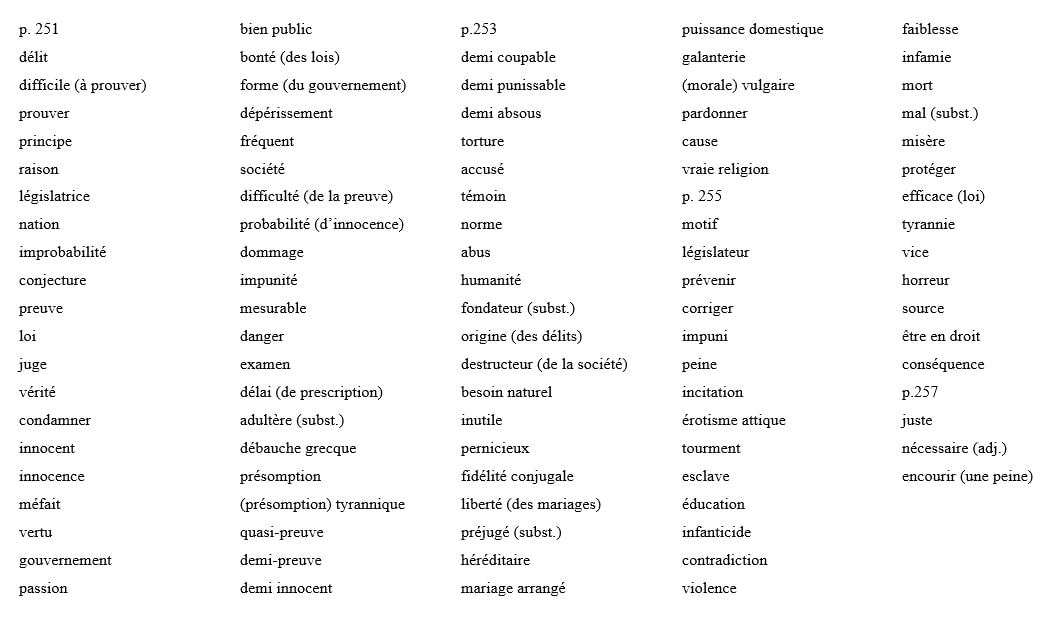
\includegraphics[width=16cm]{Partie3/images/chap2/termes_cles1.jpg}}
    \caption{Liste des termes clés choisis en français du chapitre 30/31/36 du \emph{Traité}\index{Traite des delits et des peines@Traité des délits et des peines} de Beccaria\index{Beccaria, marquis de}}
    \label{fig:termes_cles1}
\end{figure}
Ensuite, les mots relevés dans le texte ont été transformés pour conserver seulement leur lemme (c'est-à-dire leur version au masculin singulier, à l'infinitif, etc., en fonction de la catégorie grammaticale) pour que cela soit plus adéquat pour une exploitation future. L'action suivante a consisté à aller rechercher les équivalents dans les autres langues, en prenant pour appui la version de 1766 de Beccaria\index{Beccaria, marquis de} pour l'italien et une version contemporaine de 1966 pour l'allemand (l'anglais n'a pas été traité dans son tableau). En conséquence, le résultat obtenu est une liste multilingue contenant tous les termes considérés comme pertinents pour nos futures analyses.

Cette liste compte un peu moins d'une centaine de mots ou expressions lexicales relatifs au droit et au sujet traité dans le chapitre 30/31/36 pris en compte pour l'établissement de cette liste.
\begin{figure}[H]
    \centering
    \fbox{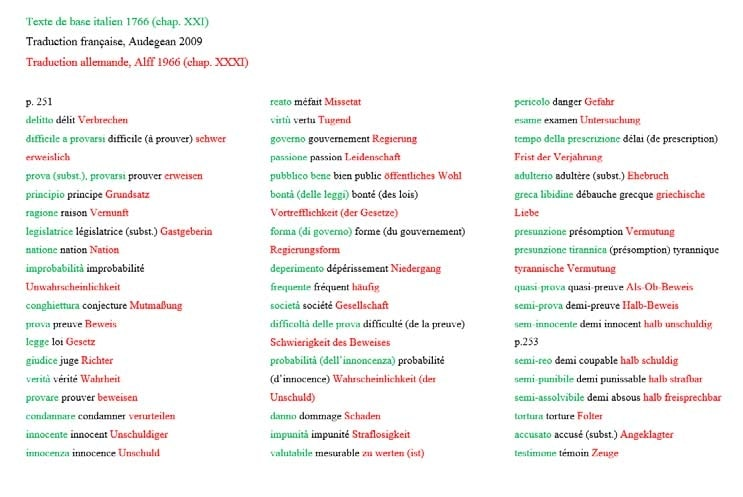
\includegraphics[width=16cm]{Partie3/images/chap2/termes_cles2.jpg}}
    \caption{Première partie de la liste de termes clés établie par Claudine Moulin}
    \label{fig:termes_cles2}
\end{figure}

\subsection{Comment perfectionner la liste~: séries de modifications à apporter}
La liste de termes noyaux nécessite des changements car elle ne correspond pas tout à fait à ce que nous rechercherons. Si l'édition modèle utilisée pour l'italien fonctionne bien car elle date de 1766, les deux autres versions posent problèmes car l'allemand et le français sont issus d'éditions contemporaines. Il est donc nécessaire de repartir vers les éditions d'avant 1800 pour chercher les expressions ou mots avec une correspondance exacte dans le fond du texte et intégrer dans la liste l'anglais, qui fait également partie de notre étude.

\subsubsection{Choisir une édition modèle pour chaque langue}
Le meilleur moyen de récupérer des expressions correctes est de choisir une édition modèle pour chaque langue et d'effectuer une lecture attentive du texte~; dans mon cas, j'ai choisi de faire une lecture phrase par phrase entre les différentes langues pour trouver exactement le terme choisi par les traducteurs dans les autres langues.

Ainsi, en italien, l'édition modèle est celle de 1766 (it5)\footcite{it5}, qui contient les nouvelles petites modifications apportées par Beccaria\index{Beccaria, marquis de}. Pour chercher les équivalences des termes en français, j'ai décidé de choisir comme modèle l'édition de 1773 (fr2-1)\footcite{fr2-1}, qui n'est pas une des versions de Morellet\index{Morellet, Andre@Morellet, André} et qui correspond donc en matière d'ordre des phrases et de structures à ce qu'avait écrit Beccaria\index{Beccaria, marquis de}. Pour l'anglais, toutes les versions étant à peu près les mêmes et suivant toute la structure de la publication originale des Beccaria\index{Beccaria, marquis de}, j'ai choisi au hasard l'édition de 1769 (ang1-2)\footcite{ang1-2} comme modèle. N'ayant pas les compétences pour travailler avec l'allemand, je ne me suis pas chargée de l'ajouter dans la liste\footnote{Les éditions allemandes ne figurent pas non plus dans l'étude des textes par la suite ou dans l'alignement partiel\index{Alignement!alignement partiel}}. Cependant, aux vues de ce qui a été observé dans la partie précédente, la version de 1767 (all3-1)\footcite{all3-1} est probablement la plus adaptée pour une lecture de comparaison, car elle reprend à peu près la structure originale du Beccaria\index{Beccaria, marquis de} et ne possède pas de très longues notes de bas de page, comme cela est le cas pour les éditions suivantes.

\subsubsection{Récupérer les homologues entre les langues}
A partir de cela, je me suis donc occupée d'aller rechercher les équivalents pour chaque langue. La méthode d'une lecture phrase par phrase est particulièrement utile pour cette démarche, puisque je suis allée chercher dans le texte italien le mot inscrit dans la liste de départ et j'ai ensuite fait en sorte de trouver exactement la même phrase mais dans la version traduite, pour avoir le mot correspondant. Cela est assez aisé puisque le mot est généralement exactement le même dans une autre langue ou correspond tout à fait à l'information qui avait été tirée du Audegean de 2009. Cependant, cela n'est pas toujours le cas et il est possible de rencontrer certains obstacles dans la réalisation de cette liste. Nous verrons par la suite ceux qui représentent plutôt des bons ou mauvais exemples d'analyse et d'autres qui présentent des difficultés car ils sont en plusieurs mots là où l'italien n'en a qu'un ou inversement. 

Un des obstacles à mentionner ici est celui du cas où les autres langues n'ont pas d'équivalence. L'exemple possible ici est celui d'\og~origine (della pene)~\fg{}. Nous retrouvons ce terme-là dans la version italienne mais il ne réapparaît pas dans les versions françaises et anglaises. En effet, les traducteurs ont changé la tournure de la phrase, menant à un rendu contenant la majorité des éléments de la phrase d'origine mais pas la partie sur l'origine des peines. Nous trouvons deux autres cas similaires avec \og~norma~\fg{}/\og~règle~\fg{} et \og~legislatore~\fg{}/\og~législation~\fg{}, qui n'ont pas d'équivalent dans la version anglaise, soit dû à une tournure de phrase différente, soit à une disparition du mot. Dans le cas de ce genre d'expression ou de mot, nous avons réfléchi à les conserver ou à ne pas les prendre en compte~; finalement, le choix s'est porté sur la première proposition. Les mots figurent dans la liste mais ils ne possèdent aucun équivalent, ce qui sera intéressant à observer pour réfléchir aux suppressions ou remplacements entre deux versions.

On regroupe alors tout ce qui a été relevé, de même que les changements, pour établir une liste multilingue de ces termes.

\subsection{Établissement d'une liste à partir du lexique juridique du corpus}
Nous avons donc effectué les modifications dans la liste de mots depuis ce qu'avait déjà produit Claudine Moulin et nous disposons alors d'une liste qui contient divers types d'équivalence.

Tout d'abord, nous trouvons des mots/expressions qui sont une traduction littérale ou quasi littérale de la version italienne. En termes de traduction exacte, nous pouvons donner comme exemple \textit{legge} qui est \textit{loi} en français et \textit{law} en anglais. Dans les cas de traductions presque identiques, nous trouvons des différences dans la catégorie grammaticale du mot~: le meilleur exemple à donner de cela est dans le titre même du chapitre. L'anglais et l'italien intitulent le chapitre \og~crimes of difficult proof~\fg{} et \og~delitti di prova difficile~\fg{} alors que le français l'intitule \og~délits/crimes difficiles à prouver/constater~\fg{}. Le français effectue une verbalisation du nom commun que nous observons pour les deux autres langues.

Ensuite, nous avons des cas où deux mots différents ont la même traduction dans une autre langue, c'est-à-dire que dans ce cas, la langue ne fait pas de distinction dans son vocabulaire entre ses termes, ce qui est quelque chose qu'il y a à de nombreuses reprises pour le cas de l'anglais. Le terme \textit{crime} est utilisé pour un crime et pour un délit, le terme \textit{law} est utilisé pour la législation et la loi et le terme \textit{destruction} est utilisé pour la destruction et le dépérissement. Ce genre de situation posera notamment quelques problèmes par la suite, lorsqu'il faudra définir des identifiants pour chacun des termes et les inscrire de manière automatique, ce qui ne fonctionnera pas toujours à cause de cela.

On trouve également l'effet inverse dans les traductions, à savoir un mot dans une langue possède plusieurs termes dans une autre, et cela est le cas pour toutes les versions. Pour en citer quelques-uns, il est fait mention d'\textit{état} et de \textit{nation} en français, là où \textit{nazioni} et \textit{nation} suffisent en italien et anglais~; \textit{greca libidine} et \textit{attica venere} en italien pour \textit{pédérastie} (fr) et \textit{sodomy} (en). Il y a même un cas où toutes les versions utilisent deux termes pour la même chose~: \textit{mankind} et \textit{human nature} (en), \textit{nature humaine} et \textit{humanité} (fr), \textit{uomò} et \textit{umanità} (it). Similairement à cet effet, nous avons également un cas où un seul mot correspond à une expression entière comme c'est le cas pour \textit{infanticide}/\textit{infanticidio} qui se traduit en anglais par \textit{murder of bastard-children}.

Enfin, nous trouvons des cas de mots où la traduction est d'autant moins littérale qu'elle semble en plus changer quelque peu le sens de la phrase ou au minimum la force de ce qui est exprimé. Pour donner un exemple de cela, nous pouvons voir qu'en italien, l'auteur mentionne l'idée qu'il est plus facile de prévenir l'adultère que de le corriger (\textit{correggere}). Dans les versions anglaises et françaises, les traducteurs semblent avoir décidé d'être plus frappant~: 
\begin{itemize}
    \item \og~de le prévenir que de le réprimer~\fg{} (fr)
    \item \og~to prevent this crime, than to punish it~\fg{} (en)
\end{itemize}
Pour citer un autre exemple, il y a un cas où le texte mentionne un \og~dépérissement de la nation\fg{} et plus tard, une \og~destruction de la société~\fg{} en français et en italien, et en anglais, c'est le terme \textit{destruction} qui sera utilisé pour ces deux fois. Si cette utilisation est justifiée dans le deuxième cas, le mot semble plus extrême pour le premier terme. Nous retrouvons un cas similaire en français, lors du paragraphe sur l'infanticide. Les versions anglaises et italiennes évoquent la \og~mort d'un être incapable~\fg{} alors qu'en français, c'est le terme \textit{destruction} qui a été choisi plutôt que la mort, ce qui donne une intention différente, voire peut être plus violente. 

Néanmoins, ce genre de cas particuliers représente probablement l'aspect le plus intéressant même s'il impactera nos annotations, car il démontre des changements significatifs, qu'il sera essentiel de prendre en compte dans nos études. Par conséquent, à partir de cette liste, nous pouvons mettre en place le tableau de termes clés à exploiter ensuite avec des identifiants et à l'aide de fichiers de dictionnaires Python pour les démarquer dans l'encodage des textes.

\section{Préparer l'annotation~: choix des identifiants et création des dictionnaires}
Les termes clés sont maintenant définis et il est donc nécessaire de passer à l'étape suivante, qui consiste à créer des tableaux, transformés par la suite en dictionnaires, qui contiendront tous ces termes clés, leur équivalent en fonction des langues et surtout l'identifiant qui leur sera apposé, puisque c'est cet identifiant qui sera déterminant dans l'analyse textuelle suivante. 

\subsection{Quels identifiants pour les termes clés ?}
Les termes juridiques que nous avons choisi d'annoter pour notre analyse textuelle nécessitent d'être identifiés par un quelconque moyen homogène, entre les différentes langues pour pouvoir effectuer une recherche facile et rapide et de cette manière, pouvoir observer les différences, similarités et particularités entre nos textes. Nous proposons ici deux systèmes de codage pour ces identifications~: soit nous choisissons un terme clé, apposé pour le terme correspondant à chaque langue (exemple~: le terme \og~crime~\fg{} dans le cas du mot \textit{crime} (fr), \textit{crime} (en), \textit{delitti} (it), \textit{verbrechen} (de)), soit nous choisissons un identifiant numérique pour les reconnaître (exemple~: le mot \textit{crime} pour chaque langue aura comme identifiant \og~TERM2~\fg{}). Ces deux solutions sont les plus appropriées mais elles présentent chacune des inconvénients qui sont à prendre en compte lors du choix de solution.

\subsubsection{Identifiant numérique}
La solution qui consiste à choisir un identifiant numérique est intéressante car elle offre une homogénéité, avec un préfixe de base (TERM) et un numéro à apposer ensuite. Le choix du numéro se fait en fonction de l'endroit où nous trouvons le mot dans le chapitre choisi (ici le chapitre 30/31/36) et il n'y a pas de classification d'importance de mots avec ces numéros. Nous pourrons ensuite enrichir la liste grâce aux nouveaux termes obtenus avec d'autres chapitres, tout en continuant la numérotation ainsi commencée. Cependant, cette numérotation peut engendrer une difficulté pour l'étape qui vient après, c'est-à-dire l'analyse. En effet, le but est de pouvoir faire des recherches rapides pour observer quel terme est plus utilisé, est employé différemment ou a une position qui change entre les versions et il peut être compliqué d'effectuer une recherche aussi rapide avec une liste de termes numériques, si nous ne connaissons pas par c\oe ur la numérotation établie. Il serait nécessaire dans ce cas d'avoir toujours sous la main la liste correspondante des termes clés et de leur identifiant, dès que nous réaliserons des recherches. 

\subsubsection{Identifiant par termes}
L'autre solution proposée consiste à apposer un terme clé pour les versions de chaque langue, soit un identifiant universel pour le mot tel que \og~T\_law~\fg{} pour le mot \textit{loi} dans toutes les langues. Le \og~T\_~\fg{} est apposé pour montrer que nous sommes dans le terme identifiant et ensuite, nous choisissons une langue pour exprimer tous les termes clés, ici l'anglais, plus universel, et nous apposons ces identifiants sur les mots dans chaque langue. Cette solution semble plus avantageuse que la version précédente, puisqu'il sera bien plus facile de faire la recherche du terme clé dans les outils textuels si le terme à requêter est immédiatement connu. Le choix d'une langue en particulier peut cependant poser un problème, notamment dans le cas où il manque des équivalents. Pour les termes \textit{délit} et \textit{crime} par exemple, le mot était le même en anglais, donc il a fallu trouver un équivalent pour ne pas avoir le même identifiant pour deux concepts qui ne sont pas exactement les mêmes et doivent être différenciés.

\paragraph{}Ainsi, si les deux modèles pour annoter les fichiers \textsc{xml} d'une identification sont satisfaisants et sont viables dans le cas d'une étude, il sera sûrement préférable de choisir la deuxième option, qui offrira une facilité de recherche, notamment si le texte et les termes juridiques sont bien connus, puisque nous saurons dès lors exactement ce qu'il faudra aller rechercher dans le texte. De ce fait, la requête sur le logiciel \textsc{txm} pourra se faire de manière rapide et effective grâce à l'identifiant, afin d'obtenir rapidement les résultats recherchés, comme cela est démontré ci-dessous par la figure \ref{fig:requete_txm}.
\begin{figure}[H]
    \centering
    \caption{Exemple d'une requête sur \textsc{txm} avec un des identifiants choisis}
    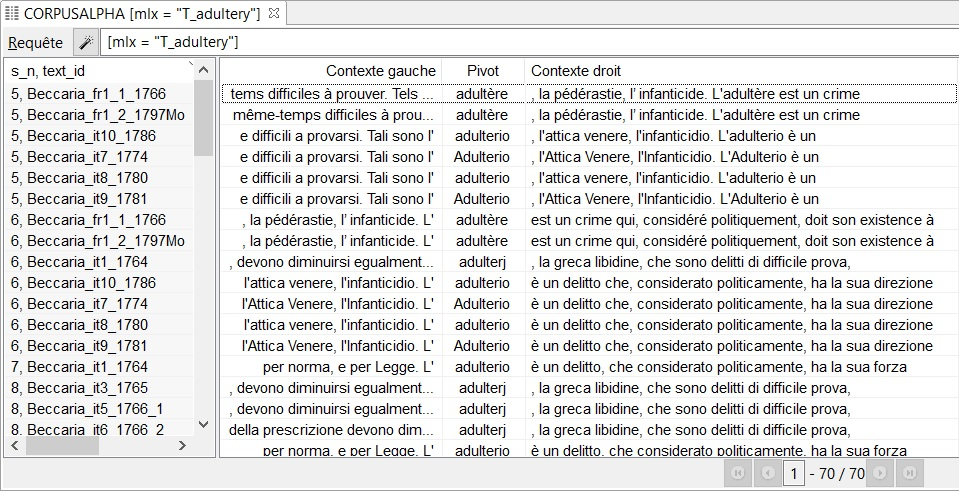
\includegraphics[width=16cm]{Partie3/images/chap2/requete_txm.jpg}
    \label{fig:requete_txm}
\end{figure}

\subsection{Créer les dictionnaires d'annotation}
Après avoir trouvé les identifiants adéquats, nous avons à disposition des listes avec un identifiant pour un mot dans trois langues différentes. L'objectif sera alors de lier ces identifiants à notre corpus pour pouvoir l'analyser et obtenir des statistiques et des données sur le texte\index{Statistique textuelle} sans prendre en compte les distinctions de langues. Pour pouvoir incorporer ces termes et leurs identifiants, il suffit de créer des dictionnaires dans des fichiers Python que nous ajouterons ensuite au texte sous son format \textsc{xml} par la rédaction d'un nouveau script. Deux dictionnaires sont mis en place, un pour chaque type d'identifiant (alphabétique et numérique) et chacun contient tous les mots séparés en trois, à l'aide de variables, que nous appellerons plus tard dans le script. Chacune des variables contient un mini-dictionnaire avec les termes et leurs identifiants pour chaque langue du corpus.

Cependant, un obstacle se présente dans la rédaction de ces dictionnaires, puisqu'un des cas expliqué lors de la présentation des termes est le fait que certaines expressions sont polylexicales, ce qui signifie que dans la mesure où notre annotation se fait dans un texte balisé mot par mot, il sera impossible de mettre l'expression en entier, puisqu'elle ne sera pas retrouvée lors de la lecture du texte et ne sera donc pas annotée. C'est pourquoi les premiers dictionnaires à établir impliquent d'opérer une pré-sélection dans les listes à disposition, avec seulement les expressions monolexicales et leurs identifiants, ce qui réduit la liste des termes. Il est possible de trouver une alternative pour les expressions restantes~: la solution serait alors de choisir un des mots de l'expression et de l'annoter avec l'identifiant. Cela a tout de même une limite dans le cas où l'expression n'aurait pas été écrite de la même façon en fonction des éditions, avec, par exemple, un tiret ou non, ce qui résultera en un balisage différent pour le \textsc{xml} et donc un encodage non complet lors de l'annotation des termes juridiques. De plus, avec un encodage de seulement un des mots, le reste de l'expression sera perdu dans la recherche, à moins de trouver un moyen d'y mettre un attribut à faire ressortir ensuite.

Les dictionnaires seront donc majoritairement composés des expressions monolexicales et par conséquent, le texte ne sera pas entièrement annoté avec le lexique juridique. Pour régler ces problèmes dans nos recherches, il est possible de requêter les expressions manquantes dans les outils à disposition pour exploiter complètement le corpus.

\paragraph{}Une fois les listes de termes juridiques établies et les dictionnaires créés, la dernière étape consiste à rédiger un script pour pouvoir inscrire ces annotations dans le corpus et ensuite procéder à diverses requêtes et extractions de données pour obtenir les informations dont nous avons besoin pour réaliser l'alignement\index{Alignement} recherché.

\section{Procéder à l'annotation~: rédaction et application du script}
L'annotation s'effectue sur un fichier \textsc{xml-tei}, qui a été produit par la plateforme \textsc{txm} lorsque nous avons importé les corpus par langue et à l'aide de son module \emph{TreeTagger}, qui lemmatise chaque forme. L'outil a décomposé le texte par mot, insérant chacun d'eux dans une balise <w>, qui a ensuite été complétée par plusieurs balises et attributs, pour apporter des détails au mot, à savoir sa forme dans le texte, sa catégorie grammatical (POS) et son lemme (LEMMA). Ceci donne une balise mot de ce type~:
\begin{minted}{xml}
<w id="w_beccaria_fr2_1_1773_33" n="33">
<txm:form>ait</txm:form>
<txm:ana resp="#txm" type="#frpos">VER:subp</txm:ana>
<txm:ana resp="#txm" type="#frlemma">avoir</txm:ana>
</w>
\end{minted}
Nous insérons par la suite nous même une forme normalisée, c'est-à-dire la forme modernisée du mot lorsque celui-ci est désuet, forme que nous avions relevé lors de la correction orthographique et de la création du dictionnaire d'enrichissement (voir figure \ref{fig:etape4}). Pour se faire, nous utilisons un script à base d'un dictionnaire et d'expressions régulières ou d'un module \textsc{xml}, effectuant la démarche suivante.
\begin{figure}[H]
    \centering
    \fbox{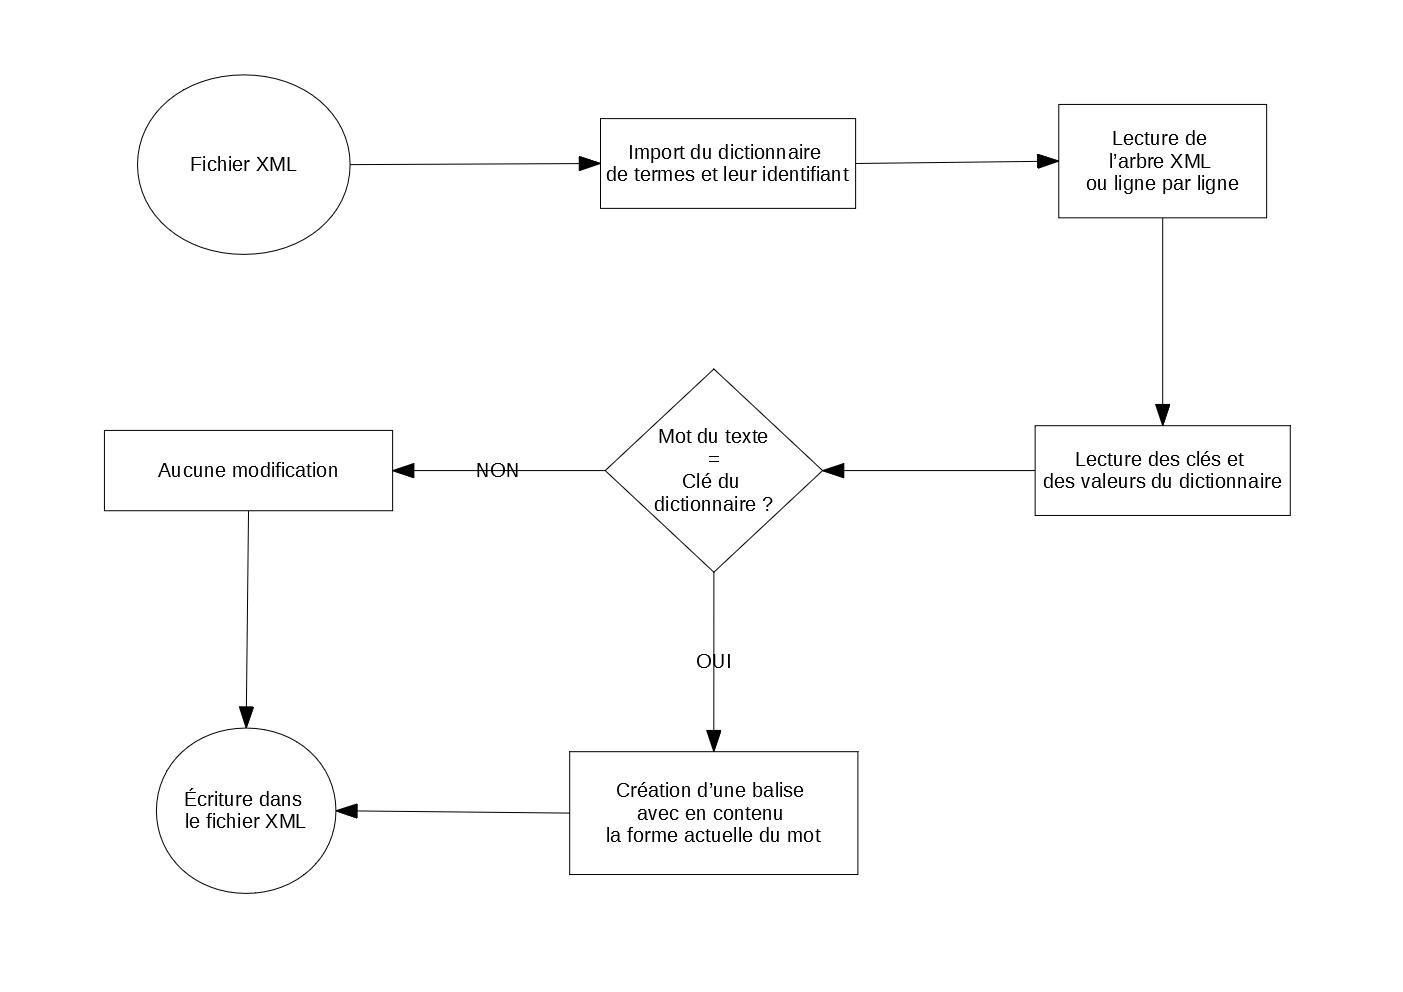
\includegraphics[width=14cm]{Partie3/schemas/normalisation_txm.jpg}}
    \caption{Diagramme d'activité montrant les étapes pour insérer une balise contenant la forme modernisée d'un mot}
    \label{fig:normalisation_txm}
\end{figure}
Partant d'un fichier \textsc{xml}, le processus de la figure \ref{fig:normalisation_txm} consistera à lire le texte et le dictionnaire à disposition, puis lorsque le système trouve un mot correspondant à une des clés du dictionnaire, un nouvel attribut est ajouté à ce mot, dont la valeur est la forme modernisée du mot. 

\paragraph{}À partir de ce fichier \textsc{xml} contenant diverses balises et attributs, nous allons procéder à une annotation en travaillant sur un rajout de balises et un changement de la valeur de l'attribut lorsque le script rencontrera une particularité que nous lui aurons spécifiée. Pour se faire, nous avons à disposition deux scripts, qui effectuent la même tâche mais en utilisant deux techniques différentes, la seconde technique (figure \ref{fig:annotation_xml}) étant une amélioration de la première (figure \ref{fig:annotation_txm}).
\begin{figure}[p]
    \centering
    \fbox{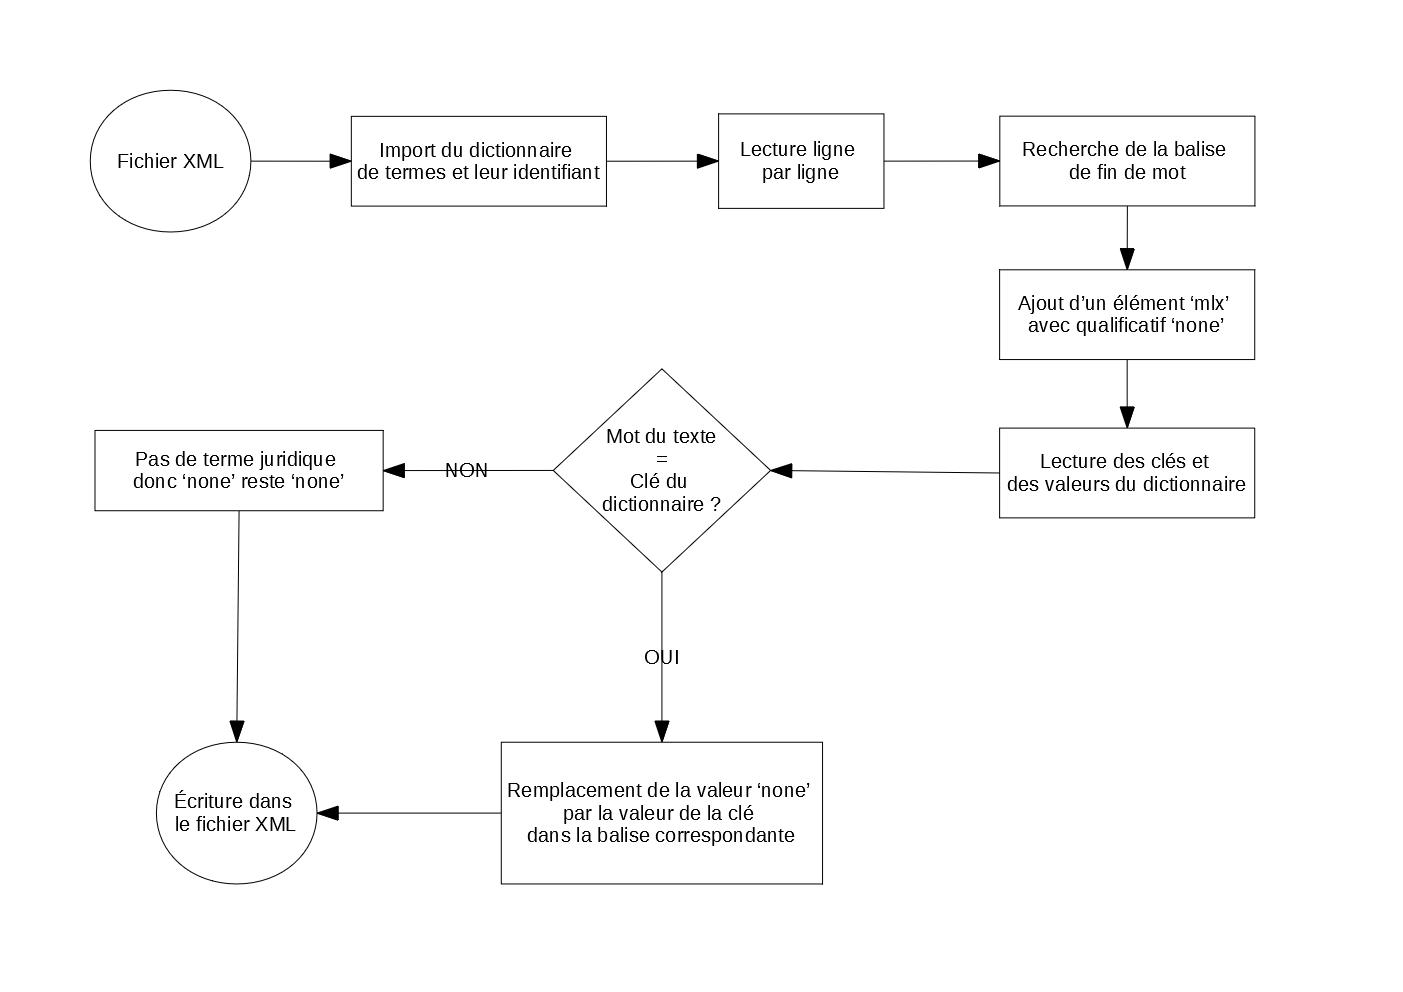
\includegraphics[width=14cm]{Partie3/schemas/annotation_txm.jpg}}
    \caption{Diagramme d'activité représentant les étapes de l'annotation du corpus sous son format \textsc{xml} en utilisant les expressions régulières}
    \label{fig:annotation_txm}
\end{figure}
\begin{figure}[p]
    \centering
    \fbox{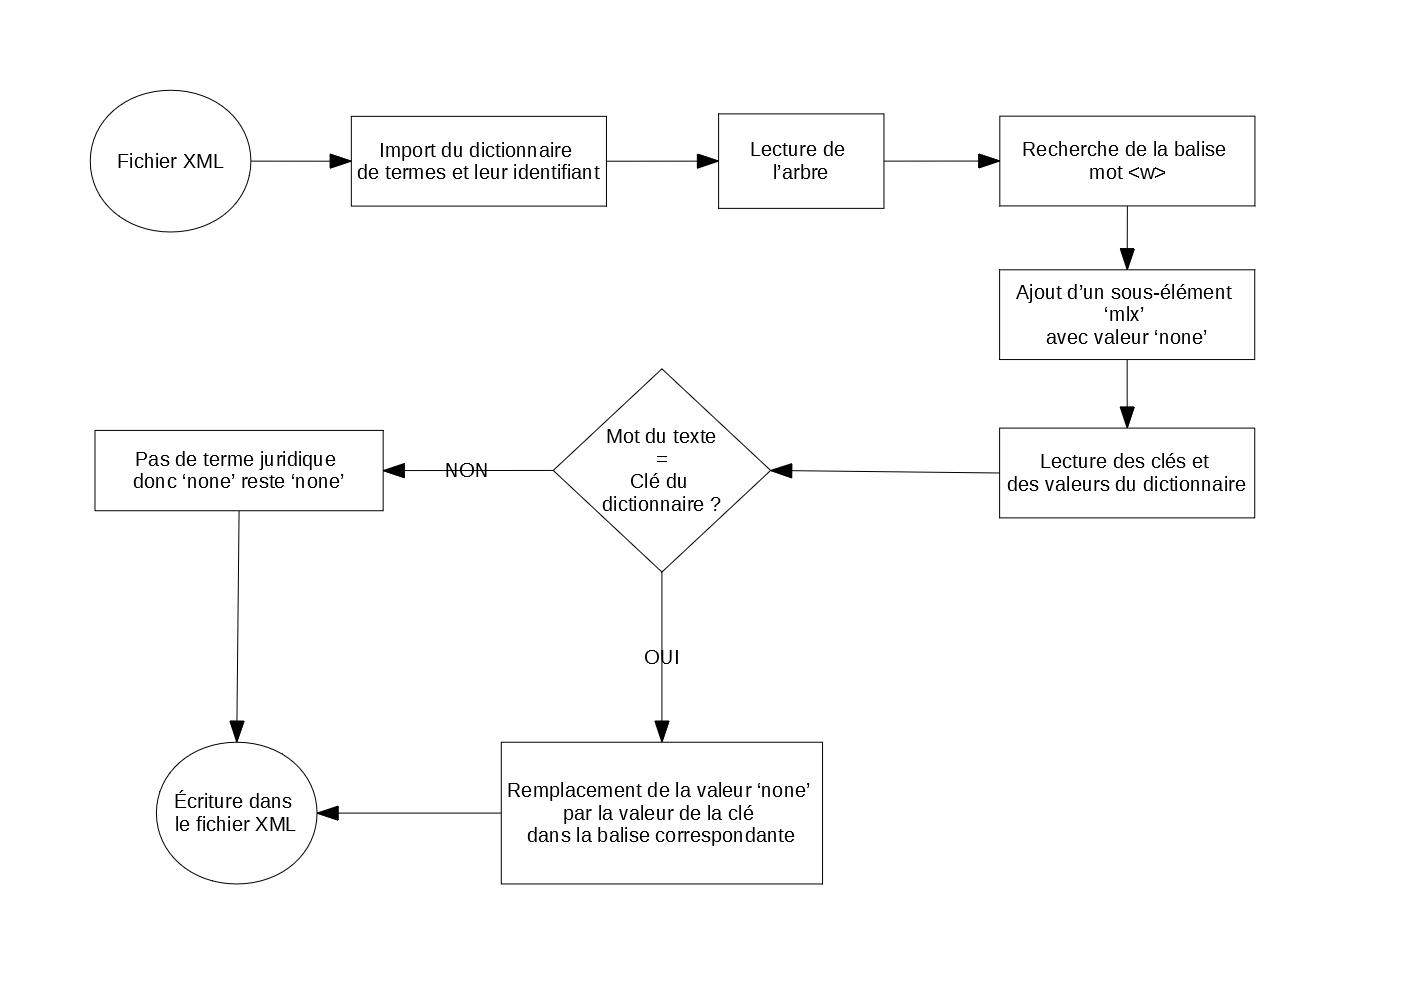
\includegraphics[width=14cm]{Partie3/schemas/annotation_xml.jpg}}
    \caption{Diagramme d'activité représentant les étapes de l'annotation du corpus sous son format \textsc{xml} en utilisant un module \textsc{xml}}
    \label{fig:annotation_xml}
\end{figure}
\paragraph{} Ce processus présente la manière dont, en partant d'un fichier \textsc{xml}, le corpus pourra être annoté des termes juridiques dont nous avons précédemment établi la liste. Dans un premier temps, le processus distribuera un attribut unique à tous les mots présents dans le texte. Dans un second temps, en effectuant à la fois une lecture des balises, de leur texte et du dictionnaire qui lui a été donné, le processus ira lire tous les mots du texte et s'il en trouve un qu'il a déjà rencontré dans le dictionnaire, il changera la valeur du nouvel attribut par la valeur qui correspond à ce qu'il a trouvé dans le dictionnaire. Enfin tout cela est inscrit dans le fichier \textsc{xml}, permettant alors d'avoir un texte annoté suivant ses termes juridiques.

\subsection{Annotations à l'aide d'expressions régulières}
Reposant principalement sur des expressions régulières, le premier script Python comporte trois étapes qui permettent d'insérer les attributs nécessaires au texte pour opérer l'annotation. Tout d'abord, le système récupère le dossier de fichiers que nous lui appelons et le dictionnaire contenu dans la variable demandée dans la requête du terminal. Ensuite, il place, pour tous les mots, juste avant la fermeture de la balise <w> et après la balise du lemme, une nouvelle balise, qui contiendra un attribut de type \textbf{mlx}, qui aura comme valeur unique \og~none~\fg{}. Une fois cela placé, le système ira lire les clés et valeurs contenues dans la variable donnée et en lisant le texte, il cherchera les correspondances aux clés. Dans le cas où il en trouve, ces clés seront contenues dans la balise du lemme et à l'aide d'une expression régulière, il changera la valeur \og~none~\fg{} par la valeur de la clé. Enfin, cela sera écrit dans un nouveau fichier \textsc{xml} contenant ces annotations.

Le positionnement est important dans le texte et dans le script, puisque la liste des termes a été établie de manière à ce que ce soit la forme lemmatisée qui soit rattachée à l'identifiant. Ainsi c'est le lemme qui est recherché dans le fichier \textsc{xml} et non la forme du mot dans le texte. Au final, l'expression régulière s'appuie sur le fait de trouver exactement le lemme dans sa balise correspondante, pour remplacer ensuite la valeur \og~none~\fg{} en la valeur de la clé. Si une balise est insérée entre le lemme et le \textbf{mlx} ou si une modification du texte change la structure du fichier \textsc{xml}, le script ne fonctionnera plus et l'annotation ne pourra pas se faire. Cela représente donc la limite majeure de l'utilisation des expressions régulières dans ce cas. C'est pour cela qu'une autre version a été développée, reposant plus sur le \textsc{xml}, lié avec du Python.

\subsection{Annotations à l'aide d'un module XML}
Python dispose de nombreux modules pour effectuer ce qui lui est demandé et parmi ceux-ci, nous pouvons retrouver un module destiné à l’utilisation de Python pour la manipulation de documents \textsc{xml}~: \emph{ElementTree}\footnote{\url{https://docs.python.org/fr/3/library/xml.etree.elementtree.html}}. Ce dernier se compose de différents éléments pour permettre de manipuler un fichier \textsc{xml}, créer des balises, en supprimer et faire des modifications dans un arbre donné.  Le script à base du module \textsc{xml} suit le même cheminement que le script d’annotations rédigé à l’aide des expressions régulières mais utilise les éléments de \emph{ElementTree}. Par conséquent, après avoir appelé le texte, dont il a lu l’arbre \textsc{xml}, et le dictionnaire associé, ainsi qu’après avoir défini les \textit{namespaces}\footnote{Espace de noms \textsc{xml} qui permet d'employer des éléments et des attributs nommés dans une instance \textsc{xml}} qui se trouvent dans le fichier \textsc{xml}, nous allons chercher, à l’aide d’une boucle, le contenu et les sous-éléments de la balise mot <w>, par le biais de l’élément \textit{iterfind}\footnote{\url{https://docs.python.org/fr/3/library/xml.etree.elementtree.html\#xml.etree.ElementTree.Element.iterfind}}. Nous enrichissons alors cette balise d'un sous élément (\textit{ET.SubElement}\footnote{\url{https://docs.python.org/fr/3/library/xml.etree.elementtree.html\#xml.etree.ElementTree.SubElement}}), pour lequel nous définissons des attributs et une valeur qui sera égale à \og~none~\fg{}. Par la suite, après avoir appelé les clés et valeurs du dictionnaire, le processus consistera à aller chercher dans les valeurs de toutes les balises enfants de <w> (\textit{itertext()}\footnote{\url{https://docs.python.org/fr/3/library/xml.etree.elementtree.html\#xml.etree.ElementTree.Element.itertext}}) ce qui est identique à une des clés du dictionnaire. Lorsque c’est le cas, nous lui faisons simplement changer la valeur \og~none~\fg{} de la balise définie plus tôt. Une fois cela fait, tout est écrit dans l’arbre et le nouveau fichier \textsc{xml} est créé, en contenant les annotations juridiques voulues. 

Cette méthode est plus sûre que la première, car les éléments exacts de l’arbre sont donnés et dans le cas où il y a un changement d’ordre des balises, ce script fonctionnera toujours contrairement au précédent, car il saura exactement quoi aller chercher. La lecture est également plus aisée ici puisque nous lui faisons chercher par balise et par contenu de balise, donc le script est plus simple et plus approprié au texte à disposition.

\paragraph{}Ainsi, à l'aide de l'un ou l'autre des scripts, nous pouvons ajouter les annotations dans le texte sous son format \textsc{xml}, ce qui, couplé avec la balise de normalisation lorsqu'elle est nécessaire, donne un résultat comme cela~:
\begin{minted}{xml}
<w id="w_beccaria_fr2_1_1773_93" n="93">
<txm:form>loix</txm:form>
<txm:ana resp="#txm" type="#norm">lois</txm:ana>
<txm:ana resp="#txm" type="#frpos">NOM</txm:ana>
<txm:ana resp="#txm" type="#frlemma">loi</txm:ana>
<txm:ana resp="#txm" type="#mlx">T_law</txm:ana>
</w>
\end{minted}
Avec cela, nous avons un fichier \textsc{xml-tei} agrémenté, notamment pour que ressorte aisément son lexique juridique, essentiel pour l'étude du texte et l'analyse des différentes versions. En effet, ces annotations nous permettent d'étudier d'une manière différente le texte. Nous avons maintenant la possibilité de travailler le corpus entièrement, sans distinction de langues, puisque l'analyse se basera sur les annotations qui ont un identifiant unique pour les trois versions. En l'état, même si les langues seront différentes, il sera possible d'observer les contextes d'utilisation des termes juridiques, de noter leurs fréquences d'utilisation par année ou par langue et d'effectuer divers autres types d'analyses statistiques\index{Statistique textuelle}, en plus des analyses simples par sous-corpus de langues. Nous pourrons donc procéder à cela et ultérieurement, à partir des données recueillies, obtenir un alignement partiel\index{Alignement!alignement partiel} ciblé\index{Alignement!alignement cible@alignement ciblé} grâce à ce lexique.
\chapter{Exploitation du contenu des corpus par les statistiques textuelles}
\fancyhead[LO, RE]{Exploitation du contenu}

Avant d'arriver à la finalité de notre projet, il est essentiel d'explorer tous les textes que nous avons à disposition et pas seulement le corpus enrichi que nous venons de mettre en place. Cela nous permet de récupérer de plus amples informations sur le texte et sa composition, afin d'étudier son contenu mais aussi trouver les meilleurs moyens d'analyse de corpus pour créer notre alignement\index{Alignement}. Nous pouvons ainsi déjà nous avancer sur notre objectif en travaillant notamment le lexique des chapitres, mais aussi les différences entre les chapitres et entre les langues, travail qui est au c\oe ur de notre analyse du \emph{Traité\index{Traite des delits et des peines@Traité des délits et des peines}} de Beccaria. Notre démarche consistera donc à expliquer la manière dont s'étudie un texte par les statistiques, puis à introduire deux modules pour effectuer cette exploration et enfin présenter plusieurs fonctionnalités pour dégager diverses données à propos des textes de notre corpus. 

\section{L'analyse statistique des données textuelles\index{Statistique textuelle}, une autre manière d'étudier un corpus}
Afin d'étendre le domaine de l'étude de texte, il est essentiel de trouver de nouvelles manières d'explorer complètement un corpus. Pour se faire, il est intéressant de se tourner vers d'autres disciplines, de manière à combiner notre propre champ d'études avec d'autres probablement plus inattendus. C'est ainsi que s'est développée l'analyse statistique des données textuelles, mêlant l'étude de texte à des mathématiques.

\subsection{Des mathématiques pour réaliser une analyse textuelle}
La statistique textuelle est une méthode qui se trouve à la croisée de plusieurs disciplines et tient son origine du développement d'un nouveau moyen d'analyse de texte, qui utilise les mathématiques. Diverses recherches ont été effectuées sur des textes et des ouvrages en prenant en compte des éléments statistiques, tels que des fréquences et des cooccurrences et plusieurs lois de probabilité ont alors été énoncées. La première et plus importante est la loi d'Estoup-Zipf, plus tard devenue loi de Zipf-Mandelbrod. Elle porte sur la fréquence d'un mot dans un texte et montre que cela suit un schéma, où le rang du mot dépend du nombre de fois où il apparaît dans le texte. Ce schéma a été déterminé après l'observation de l'ouvrage de James Joyce, \emph{Ulysse}. En comptant les occurences de mots, Zipf a découvert que le mot le plus courant revenait 8 000 fois, le dixième 800 fois, le centième 80 fois et le millième 8 fois, ce qui lui a inspiré la loi. Cette loi a ensuite été peaufinée par le mathématicien français Benoît Mandelbrot, qui a rajouté un coefficient, qui ira prendre en compte les mots-vides qui sont les mots très fréquents qui faussent la courbe. Il a également rajouté deux paramètres, à savoir le type de texte et la langue étudiée, afin que la loi puisse s'adapter. Cette correction a permis de parfaire le résultat, qui est alors exact, et cette loi a ouvert la voie ensuite à de multiples autres lois ou formules mathématiques qui s'appliquent à l'analyse d'un texte. Dans ce cadre, nous pouvons citer la loi de Heaps qui s'interroge sur la probabilité de l'apparition d'un nouveau mot dans un texte et la contagion qui est la probabilité qu'un mot réapparaisse après l'avoir vu une première fois. Ces deux méthodes peuvent se lier entre elles puisqu'il peut être intéressant d'étudier si un mot apparaîtra et ensuite combien de fois il le fait. Ces méthodes statistiques ont par la suite été étendues pour une étude multi corpus, comme avec la boite à moustache qui s'intéresse à l'apparition du mot à travers plusieurs textes (minimum, maximum, quart 1, quart 3 et médiane). La répartition qui sera donnée avec la boîte à moustache permettra de savoir s'il y a une spécificité en fonction d'un texte du corpus, si un mot est plus utilisé dans un des textes que dans un autre. Cela a, par exemple, été utilisé avec des \oe uvres de théâtres de quatre auteurs~: Pierre et Thomas Corneille, Molière et Scarron. La recherche s'est faite sur la fréquence d'apparition d'un mot choisi au préalable dans tous les textes de ces auteurs.

Ces méthodes ont par la suite été perfectionnées, augmentées et développées de manière à être plus accessibles et plus aisées d'utilisation pour les historiens, les linguistes et d'autres praticiens des sciences sociales, les mathématiques brutes n'étant pas toujours facilement exploitables.

\subsection{Une abondance d'outils pour opérer l'analyse statistique des données\index{Statistique textuelle}}
L'essor de l'informatique dans les disciplines des sciences sociales et des lettres a permis le développement de nouvelles techniques et notamment la mise en place d'outils pour traiter les données textuelles. Il y en a eu un très grand nombre de créés qui n'ont pas tous la même fonction, ni le même angle de travail, en fonction de leur approche du corpus de texte et des méthodes statistiques. Si la démarche n’est pas la même, les procédures se ressemblent, telles que le calcul de spécificité lexicale ou l’analyse des concordances\footcite[p.~33-36]{stat_text_garnier}. La forme sous laquelle se présente le corpus est également importante et l’une des plus significatives, qui sera également essentielle dans notre travail, est la lemmatisation. Elle consiste à regrouper des mots selon une forme plus basique et ainsi à \og~ ramener un verbe conjugué à son infinitif, rassembler les formes au pluriel et au singulier, les masculins et féminins, et plus généralement regrouper les formes qui correspondent à une même racine, avec des désinences différentes\footcite[p.~867]{stat_text_guerin}.~\fg{}. La lemmatisation est utilisée et favorisée par la majorité de ceux qui effectuent les statistiques textuelles\index{Statistique textuelle} et elle est ainsi parfois insérée directement lors de l'import d'un corpus en fonction de l'outil à disposition, ce qui permet d'avoir plus de résultats d'analyse lors des recherches sur le logiciel.

Il existe un certain nombre de logiciels de statistiques textuelles\index{Statistique textuelle} et même si une concurrence existe, ils sont assez variés pour que certains soient plus aisés à utiliser selon le type de corpus qui est soumis. Parmi ceux-ci, nous pouvons en citer trois de références~: \textsc{spad} (Système Portable pour l'Analyse des Données Textuelles) contient un module spécifique dédié aux données textuelles et est davantage adapté aux textes courts~; \textsc{alceste} (Analyse des Lexèmes Cooccurrents dans les Énoncés Simples d'un Texte) a été conçu pour le traitement des données textuelles et pour des corpus de taille plutôt importante~; \textsc{lexico} est assez proche de \textsc{spad} et possède une interface avant tout visuelle\footcite[p.~33-36]{stat_text_garnier}. Ces trois logiciels possèdent tous une lemmatisation automatique qui est parfois assistée d'options plus avancées. Parmi les autres logiciels, nous pouvons également mentionner le logiciel \textsc{rstudio} qui fait du comptage de mots mais qui est principalement un logiciel statistique et graphique s'appuyant beaucoup sur de la programmation. Plus récemment, en 2010, une nouvelle plateforme logicielle en open-source a fait son apparition~: \textsc{txm}\footcite{txm_plateforme}. \textsc{txm} offre des fonctionnalités similaires aux logiciels précédemment cités, certaines des requêtes peuvent d'ailleurs être faites avec le langage de programme \textsc{r}, qui fait tourner le logiciel \textsc{rstudio} et offre également la possibilité de produire le corpus sous de nombreuses formes (\textsc{txt}, \textsc{doc}, \textsc{odt} ou encore \textsc{xml-tei}). Ce logiciel opère une lemmatisation automatique, qu'il est possible d'utiliser par la suite pour les requêtes et permet également d'effectuer ses propres annotations sur le corpus à disposition.

Ainsi, ces divers logiciels rendent possible un travail plus aisé selon le corpus qu'il faut manipuler et encouragent une diversité d'analyses sur un corpus, car cela peut alors faire ressortir des informations ou des données que d'autres types d'analyses n'auraient pas relevées.  Dans le cadre de notre étude de texte, le choix de logiciels s'est porté sur \textsc{txm} et \textsc{rstudio}, avec lesquels nous allons effectuer diverses analyses pour explorer notre corpus.

\section{Analyser les textes de notre corpus~: import et manipulation à l'aide de logiciels de statistiques textuelles\index{Statistique textuelle}}
Avant de pouvoir réaliser nos analyses avec \textsc{txm} et \textsc{rstudio}, il est nécessaire d'importer le corpus sur chacun des logiciels et d'apporter certains éléments, dont notamment un fichier de métadonnées, de manière à pouvoir ensuite travailler avec les textes à disposition. Cet import sera différent en fonction des logiciels, du fait de leurs caractéristiques propres.

\subsection{TXM~: un import simple et rapide, dépendant du type de fichier}
Notre travail avec \textsc{txm} s'effectue en deux temps et avec deux formes différentes du corpus. Cela nécessite donc deux imports distincts, qui ne solliciteront pas les mêmes éléments et ne demanderont pas la même charge de travail.

Dans un premier temps, il est nécessaire d'effectuer un import simple du corpus par langue et avec les divers chapitres que nous avons océrisés\index{OCR!ocerisation@océrisation}, mis en forme et corrigés. Ces fichiers, existant au format \textsc{txt}, ne nécessitent qu'un élément supplémentaire afin de pouvoir être importé sur le logiciel \textsc{txm}~: un fichier de métadonnées. Effectivement, l'interface \textsc{txm} possède plusieurs styles d'import et les fichiers de textes brut ou fichier word et certains fichiers en \textsc{xml} demandent un \textsc{csv}, qui contiendra les informations sur l'identifiant du document importé, ainsi que sa langue et sa date, dans l'intention d'avoir des données précises lorsqu'elle créera le corpus que nous manipulerons. L'identification de ces données lui permettra ensuite de trier nos documents grâce à ces métadonnées, pour créer des sous-corpus, des partitions ou établir certaines statistiques suivant ces critères. Une fois que le fichier \textsc{csv} contient les métadonnées correspondant au corpus soumis, il est possible d'importer ce corpus et \textsc{txm} peut ensuite procéder à diverses opérations avec les textes fournis.

Extérieurement, le logiciel \textsc{txm} ne semble procéder qu'à un import de corpus que nous pouvons ensuite utiliser. Intérieurement, il effectue de nombreuses opérations qui visent à présenter le texte sous de nouvelles formes et avec de nouveaux encodages, afin de maximiser les capacités d'analyse. L'une de ces modifications principales, que nous avons longuement étudiée dans le chapitre précédent, vise à modifier le texte afin qu'il soit encodé au format \textsc{xml-tei} et balisé mot par mot, avec un enrichissement pour chacun des mots d'attributs sur sa catégorie grammaticale et lexicale, offrant ainsi plus de statistiques, sur des données inédites. C'est ce type de fichier que nous utiliserons dans un deuxième temps et cette fois-ci en effectuant un import de corpus multilingue\index{Alignement!corpus multilingue}. Comme nous l'avons expliqué dans le chapitre \ref{chap_annotations}, nous avons modifié ce fichier encodé en intégrant de nouvelles balises, dont notamment une avec un attribut \textit{mlx} qui relève les mots du texte qui contiennent des termes juridiques, fil conducteur de notre analyse dans notre objectif d'alignement\index{Alignement}. Ainsi, une fois les fichiers modifiés pour contenir les nouvelles balises, nous allons pouvoir les importer sur le logiciel \textsc{txm} puisque ce dernier possède également un mode d'import pour ces types de fichiers~: \textsc{xml-tei txm}. Cette fonction permet en résumé de réimporter dans le logiciel un texte qu'il a lui-même balisé avec des attributs qui contiennent l'information que le document a été encodé par \textsc{txm} (exemple~: \mintinline{xml}{<txm:ana resp="#txm" type="#frpos">}). À partir de là, il est important de vérifier la langue que le logiciel choisira pour importer le corpus. Il est possible de lui imposer de deviner la langue du texte. Cette fonctionnalité est disponible à chaque import de corpus mais n'aurait pas fait sens lors du premier import que nous avons mentionné, puisque, ici, nous avons un moyen de rechercher des informations à travers un corpus multilingue\index{Alignement!corpus multilingue}, ce qui n'était pas le cas lorsque les documents étaient seulement des fichiers .txt. En devinant la langue du corpus, il prend en compte les distinctions qu'auront les textes vis-à-vis de leur attribut mais pourra tout de même les traiter comme un tout. Il sera possible de travailler selon ces spécificités ou selon les caractéristiques communes à tous les textes.

Il est donc possible avec \textsc{txm} d'étudier des textes sous différents formats, diverses langues ou avec plusieurs annotations pour explorer au mieux le texte grâce à la multitude de fonctionnalités proposées. Nous pourrons observer les différents résultats que nous obtenons à propos de notre corpus et nous aurons notamment la possibilité de les comparer avec ceux que produit \textsc{rstudio}, avec le même corpus qui doit également être importé sur ce logiciel.

\subsection{RSTUDIO~: un import par de la programmation}
\textsc{rstudio} fonctionne à partir du langage de programmation \textsc{r}, qui est destiné aux statistiques et aux graphiques. Son environnement de développement intégré (IDE) propose de travailler avec une console et un terminal ainsi qu'en lien avec notre bureau~; l'import du corpus, de même que le travail qui sera fait avec, dépendra d'un script et de ses lignes de code. Le script nous a été fourni à l'occasion d'un atelier à l'\acrshort{ehess} portant sur les \og~Méthodes et pratique de la statistique textuelle\index{Statistique textuelle} avec \textsc{r}~\fg{}. La forme du corpus que nous utiliserons ici sera la même que pour le premier import sur \textsc{txm}, c'est-à-dire les fichiers au format \textsc{txt}, ainsi que le \textsc{csv} qui est également nécessaire pour \textsc{rstudio}. Le dossier de métadonnées sera ensuite lié au corpus importé. L'import sur \textsc{rstudio} est assez similaire à celui de \textsc{txm} puisqu'il faudra aller récupérer le bon dossier de fichiers et l'appeler dans la console R. Le logiciel est cependant plus limité que \textsc{txm}, puisqu'il ne peut importer qu'un certain type de fichiers, \textsc{txt} et \textsc{csv} principalement, ce qui signifie que la deuxième partie d'import de \textsc{txm} ne pourra aucunement être réalisée avec \textsc{rstudio}. Si, une fois l'import du corpus fait, \textsc{txm} s'occupait ensuite du reste, ce n'est pas le cas pour \textsc{r} puisqu'il faut arranger le corpus pour qu'il puisse faire ce que nous voulons et cela nécessite d'autres lignes de code. De ce fait, le logiciel \textsc{rstudio} requiert que le corpus et le fichier de métadonnées soient liés, puis le texte est découpé selon une unité que nous choisissons (paragraphes, phrases, etc.). Par la suite, nous créons la table lexicale qui sera la base de nos analyses et cette étape est assez particulière, puisque \textsc{r} nous offre une spécificité que nous ne retrouvons pas dans \textsc{txm}~: la suppression des mots-vides. Par ce biais, le résultat de l'étude pourra être plus précis et moins faussé par des éléments qui n'ont pas de lien avec notre recherche. Il est également possible après de créer un dictionnaire de fréquences à partir de cette table lexicale et de faire apparaître ensuite des résultats statistiques\index{Statistique textuelle}, liés à des concordances, des cooccurrences, des fréquences, etc. Une fois le corpus appelé et modifié comme voulu, il suffit de rajouter des lignes de codes en fonction des requêtes souhaitées.

\subsection*{Conclusion~: des logiciels similaires mais distincts} 
\addcontentsline{toc}{subsection}{Conclusion~: des logiciels similaires mais distincts}
\textsc{txm} et \textsc{rstudio}, comme nous avons pu le voir, offrent à peu près les mêmes éléments d'analyse sur un même corpus donné. Si \textsc{rstudio} peut prendre en compte moins de types différents de fichiers, sur la base d'un même format (\textsc{txt}), l'analyse est très similaire. Leurs fonctionnalités proposent les mêmes requêtes~: des fréquences, des lexiques, des concordances, des cooccurrences, des \acrshort{afc}, etc. Cependant, la manière dont s'obtiendront ces fonctionnalités diverge. Là où l'interface graphique de \textsc{txm} permet un accès rapide et une requête aisée de ces fonctionnalités, l'environnement de développement de \textsc{rstudio} demande une connaissance minimale en langage de programmation et en composants à appeler pour avoir la requête voulue et atteindre le résultat attendu. Néanmoins, si cela est assimilé, nous verrons que, pour certains cas, les productions de \textsc{rstudio} seront plus précises et plus exploitables que celles de \textsc{txm}.

\section{Interroger le lexique des chapitres de notre analyse~: travail sur des nuages de mots }
Parmi les outils dont nous disposons avec les logiciels statistiques\index{Statistique textuelle}, l'un d'eux nous donne la possibilité de faire ressortir le lexique qui compose chacun des chapitres que nous analysons, sous la forme d'une liste ou d'un nuage de mots, afin d'observer les éléments qui ressortent plus que d'autres et les différences entre les langues. 

\subsection{Créer le nuage de mots~: sélection du meilleur logiciel}
Pour rendre notre étude plus efficace, nous nous concentrerons sur la production de \textsc{rstudio} et non de \textsc{txm}, ce qui s'explique par deux raisons majeures. La première est le fait que \textsc{rstudio} produit ce lexique sous la forme d'un nuage de mots, avec une différence de taille en fonction de ses occurrences dans le texte, alors que \textsc{txm} produit une liste en deux colonnes~: les mots sur la première et leur fréquence sur la seconde. L'analyse sera plus aisée avec la première option grâce à l'avantage visuel que cela apporte. De plus, l'analyse sera plus concentrée puisque le nuage de mots a été délimité dans le script, par un nombre de mots maximum et une fréquence minimale. La deuxième raison tient à une spécificité que nous avons vue à propos du logiciel \textsc{r}. Lors de la création de la table lexicale, il est possible d'imposer la suppression des mots-vides, qui sont des mots tellement communs que l'indexation n'apporte rien, à l'instar des déterminants. \textsc{r} supprime ainsi ces éléments de la table lexicale et produit ensuite le nuage de mots ne contenant alors que des termes significatifs pour notre analyse. De ce fait, cela assure d'avoir un résultat plus précis puisque l'intérêt de ce genre d'étude n'est pas d'étudier tout le lexique mais plutôt de s'intéresser à ce qui doit le plus ressortir.

À partir de ce nuage de mots, nous pouvons donc effectuer des analyses dans le corpus entre les langues. Les chapitres reprenant globalement les mêmes informations qu'importe la langue, l'intérêt est d'observer si les termes varient en fonction des éditions ou si certaines langues ont plus de spécificités que d'autres. En outre, avec trois chapitres distincts du \emph{Traité\index{Traite des delits et des peines@Traité des délits et des peines}} à disposition, il sera également possible d'effectuer des comparaisons entre ces chapitres, pour voir si certains ont plus de similitudes que d'autres et même d'examiner l'étendue de leur lexique.

\subsection{Dégager des informations~: analyse des nuages de mots}
Dans un premier temps, nous nous intéresserons aux chapitres 7/13/14 et 30/31/36, pour lesquels nous avons les nuages de mots pour les trois langues que nous analysons (anglais, français et italien) et par la suite, nous concentrerons notre analyse sur la partie contenant l'introduction et les chapitres 1-2-3 pour laquelle nous n'avons que le français et l'anglais.

\subsubsection{Comparaison de deux chapitres}
\begin{figure}[t]
    \centering
    \fbox{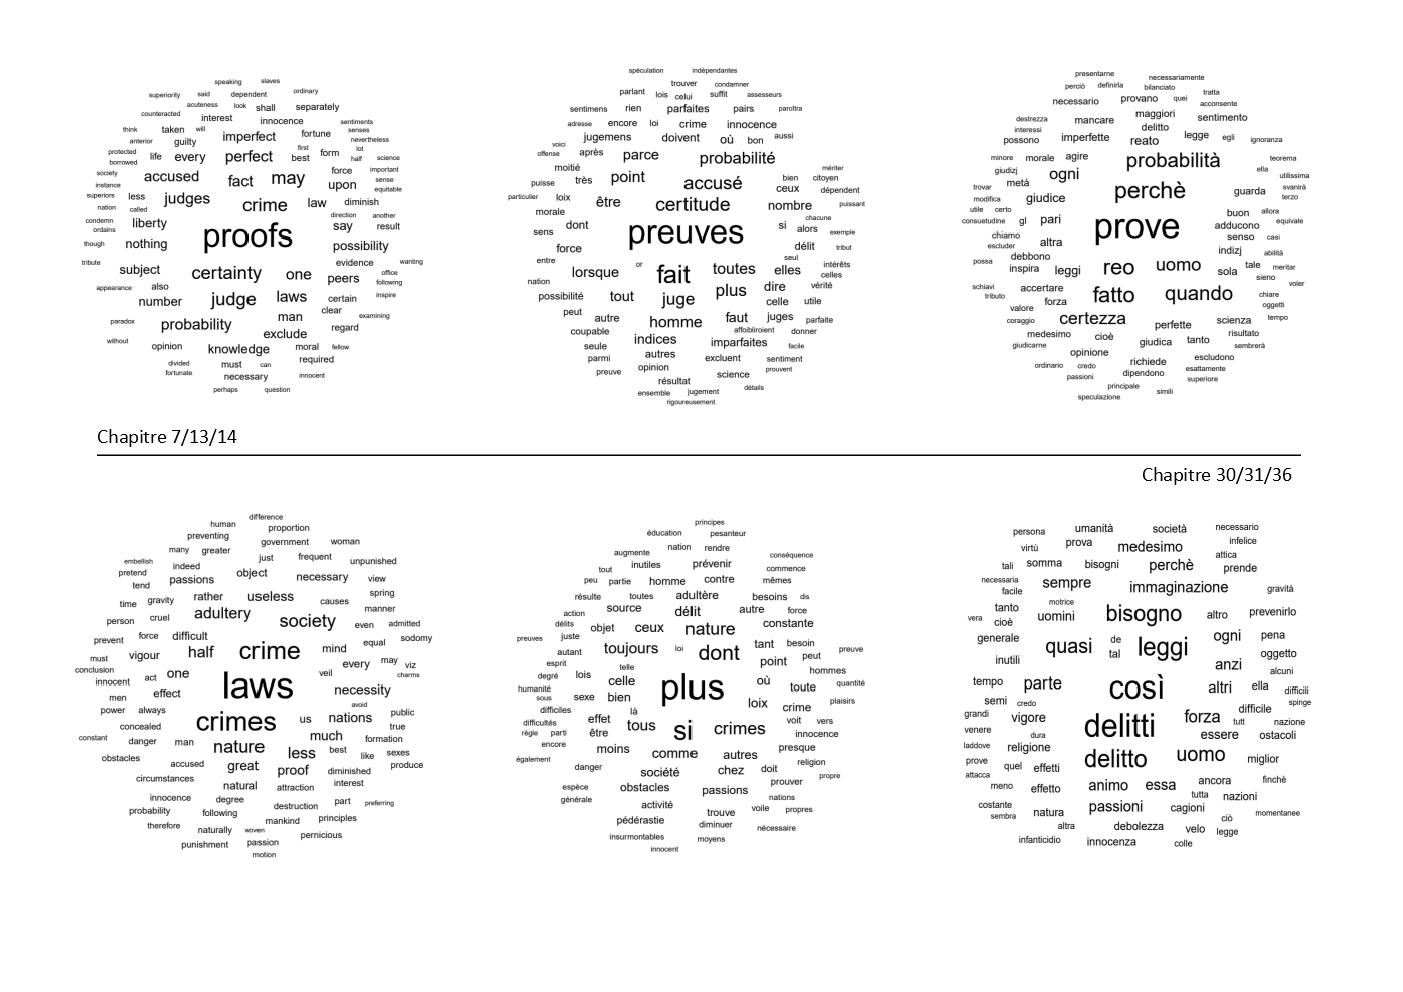
\includegraphics[width=16cm]{Partie3/images/chap3/wordcloud.jpg}}
    \caption{Nuage de mots des chapitres 7/13/14 et 30/31/36 pour les éditions anglaises, françaises et italiennes}
    \label{fig:word_cloud}
\end{figure}
Le parallèle entre les nuages de mots de ces deux chapitres est intéressant, puisque nous pouvons explicitement remarquer une différence entre les deux, simplement avec le mot le plus fréquent entre les chapitres. 

Dans la première ligne qui contient les textes du chapitre 7/13/14 dans la figure \ref{fig:word_cloud}, nous pouvons distinguer que le mot \textit{preuve} est le plus utilisé quelle que soit la langue et la taille du mot pour chacun semble montrer que la fréquence est quasiment la même qu'importe la version. Il y a donc une certaine homogénéité pour ce chapitre, comme cela peut se voir également pour les mots également très similaires qui gravitent autour de \textit{preuve}. Il est possible de citer \textit{certitude}, \textit{probabilité}, \textit{fait} ou \textit{homme} bien que ce dernier mot soit moins présent que les autres. De même pour des mots de taille moins conséquente dans le nuage, le vocabulaire est très similaire en fonction des versions. Cela laisse à penser que dans le cas de ce chapitre, il y a eu une traduction assez fidèle entre les éditions, offrant donc des nuages de mots très semblables.

À l'inverse, cette homogénéité ne se retrouve pas du tout pour le chapitre 30/31/36 sur la deuxième ligne de la même figure. Le mot le plus important n'est le même pour aucun des cas, bien que cela soit en partie dû à \textsc{rstudio}. Si les mots-vides ont effectivement été supprimés, les nuages de mots pour le chapitre en français et en italien montrent comme terme ayant la fréquence la plus importante respectivement \textit{plus} et \textit{così}\footnote{Traduction française : si}. Bien qu'il soit possible que la présence conséquente de ces mots indique un sens particulier du chapitre, celui-ci n'est pas assez explicite pour l'étude que nous effectuons et cela semble plutôt fausser le résultat du nuage. Cependant, si nous enlevons dans notre réflexion ces mots pour retrouver des termes plus éloquents, l'homogénéité n'est toujours pas présente. Le mot le plus utilisé est~: \textit{laws} pour l'anglais, \textit{nature} ou \textit{crimes} pour le français et \textit{delitti} pour l'italien. Nous sommes dans un champ lexical proche si nous considérons que \textit{crimes} est le plus utilisé en français, champ lexical qui semble d'ailleurs suivre les mots contenus dans la liste de termes définie dans le chapitre précédent et il est possible d'expliquer ce résultat. Bien que \textit{loi} ne soit pas le plus utilisé pour le français et l'italien, il reste tout de même un mot important dans ce chapitre. Nous pouvons observer que \textit{leggi} est d'une taille plutôt conséquente dans le nuage de mot de l'italien. Le cas du français est plus particulier en raison d'une différence d'orthographe~: loi s'écrit de trois manières dans les éditions françaises du corpus, \textit{loi} au singulier, \textit{lois} et \textit{loix} au pluriel. Nous pouvons distinguer deux de ces versions à une taille relativement visible dans le nuage de mots. En étudiant le reste, nous pouvons remarquer que les mots en périphérie ne montrent pas non plus une harmonie entre les versions. Cela peut nous permettre de conclure que, si le chapitre a effectivement le même sujet, qu'importe la langue, les traducteurs ont adapté leur vocabulaire et celui-ci ne correspond pas à une traduction littérale. 

Cette étude comparative entre deux chapitres nous montre donc des différences majeures entre les deux et cela peut nous laisser supposer que les traducteurs ont pris plus de libertés, dans leur vocabulaire, lors de l'édition des chapitres 30/31/36 en français et anglais par rapport à l'italien, alors que pour le chapitre 7/13/14, ils semblent avoir traduit littéralement le chapitre. De plus, les différences de structures entre certaines des versions par le travail de l'abbé Morellet\index{Morellet, Andre@Morellet, André} peuvent fausser un peu plus les résultats, ce qui n'est pas le cas pour l'autre chapitre, puisque ce dernier n'a connu aucune modification sur le fond lors de la restructuration de l'édition française de 1766.

\subsubsection{Similitudes et différences selon la langue}
Nous pouvons faire une autre analyse de nuages de mots sur un nouvel extrait, bien que l'italien ne soit pas présent ici et il ne sera donc pas possible de savoir si les traducteurs ont suivi explicitement la version originale mais nous pourrons tout de même chercher à observer des similitudes entre les deux vocabulaires utilisés.
\begin{figure}[t]
    \centering
    \fbox{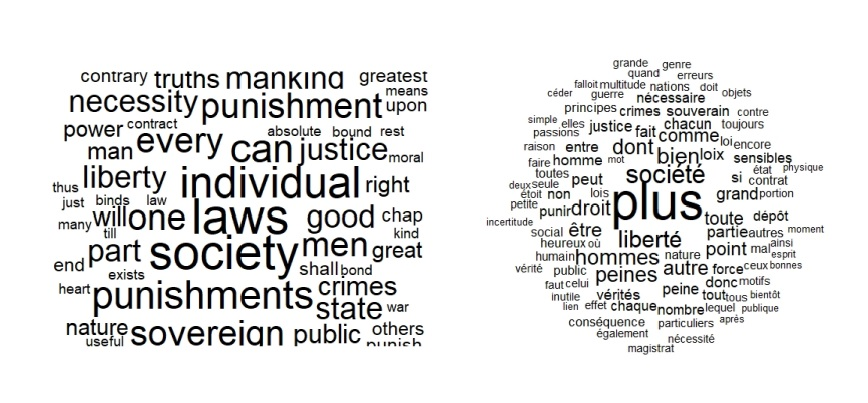
\includegraphics[width=16cm, height=8cm]{Partie3/images/chap3/wordcloud_intro.jpg}}
    \caption{Nuage de mots de la partie contenant l'introduction et les chapitres 1-2-3 pour les éditions anglaises et françaises}
    \label{fig:word_cloud_intro}
\end{figure}

En observant la figure \ref{fig:word_cloud_intro}, un élément se distingue directement~: la taille de chaque nuage de mots n'est pas équivalente. En effet, le nombre de mots maximum est de 100 et si le nuage de mots du français semble atteindre à peu près ce nombre, le nuage de mots de l'anglais semble n'en contenir que la moitié. Cela peut probablement s'expliquer par la taille des mots. En français, il y a un mot écrit largement, plusieurs mots un peu grands qui gravitent autour et d'autres mots, bien plus petits mais non de moindre importance. Dans le cas de l'anglais, nous retrouvons de très nombreux mots écrits dans une taille considérable, qui semblent prendre la majorité de l'espace du nuage de mots. En périphérie se trouve des petits mots moins présents mais non moins significatifs. L'explication du nombre de mots dans le nuage se fait par la place que prennent les mots les plus importants. Le nuage de mots est délimité par un certain espace et ainsi que l'indique \textsc{rstudio}, certains autres mots qui devaient figurer dans le nuage ne peuvent être intégrés. Cela représente une limite conséquente à cette fonctionnalité du logiciel \textsc{rstudio} mais ne crée pas de difficulté pour notre travail puisque notre intérêt ne repose que sur les mots de taille considérable. Pour le nuage de mots en français, nous avons une observation identique à celle que nous avions eu pour le chapitre 30/31/36, puisque le mot le plus fréquent est \textit{plus}. La présence de ce mot comme fréquence la plus élevée à deux reprises peut laisser supposer que \textit{plus} devrait être considéré comme un mot-vide, puisqu'il n'apporte pas d'information aux analyses et fausse le nuage de mots. En le supprimant, il serait possible de mieux discerner la place des autres mots de fréquence importante.

Une fois ces considérations prises en compte, nous pouvons comparer les nuages de mots et ce faisant, nous observons que cet extrait ne suit ni le schéma du chapitre 7/13/14, ni celui du chapitre 30/31/36. Il n'est pas homogène puisqu'il y a certains mots de taille importante dans un nuage que nous ne retrouvons pas dans l'autre mais au contraire du chapitre 30/31/36, parmi les mots importants du nuage s'observe un vocabulaire similaire tel que \textit{société/society}, \textit{loix/laws}, \textit{liberté/liberty}, \textit{souverain/sovereign}, \textit{peines/punishments}, etc. Cette comparaison nous permet également de relever que les chapitres en français semblent utiliser un lexique plus diversifié que ceux en anglais, aux vues de la différence de taille entre les mots et ce lexique traite de société, de lois et de peines, qu'importe la version.

\paragraph{}Ainsi, l'observation de ces trois chapitres différents présentés sous la forme de nuages de mots permet de nous montrer qu'il ne semble pas y avoir de réelle unité dans la manière dont sont traduits les chapitres et que les éditeurs prennent plus de libertés d'un chapitre à l'autre. Toutefois, bien que les mots ne soient pas exactement les mêmes, nous pouvons tout de même remarquer que le lexique utilisé reste similaire et cohérent en fonction des langues, laissant sa substance initiale au chapitre. Une fois ce lexique établi pour les différents chapitres que nous étudions, il sera intéressant d'analyser les liens entre ces différents mots afin de voir comment s'articule les textes.

\section{Étudier les relations de mots dans le corpus~: plusieurs méthodes pour des résultats modérément fructueux}
Élément essentiel dans les statistiques textuelles\index{Statistique textuelle}, la recherche de correspondances et de cooccurrences dans un corpus est développée grâce à de nombreux outils fournis autant par \textsc{txm} que par \textsc{r}, pour faire ressortir ces données d'une manière ou d'une autre. Cependant, même s'il existe beaucoup de méthodes, elles ne sont pas toujours concluantes ou adaptées au texte et nous allons donc observer plusieurs de ces résultats et ce qu'ils apportent ou non à notre étude.

\subsection{Explorer le texte par le biais de ses cooccurrences~: une méthode effective pour observer la structure du \emph{Traité}}
À l'aide du nuage de mots, nous avons pu observer le lexique dominant dans le corpus et les cooccurrences nous permettront de prolonger ces réflexions, puisque nous avons alors la possibilité d'observer la proximité entre ces différents mots, à savoir le vocabulaire qu'il côtoie le plus et même la manière dont s'articule le corpus. Pour réaliser cela de la meilleure manière possible, nous pourrons utiliser à la fois \textsc{r} et \textsc{txm}, qui possèdent chacun une fonctionnalité pour les cooccurrences et ces fonctionnalités peuvent se compléter pour fournir un résultat plus précis. \textsc{txm} fournit un outil simplement nommé \textbf{\textit{Cooccurrences}} qui donne la possibilité de rechercher les formes les plus proches de celle choisie pour la requête. Comme pour toutes les requêtes de \textsc{txm}, il est possible de sélectionner la propriété de la forme recherchée (mot, lemme, catégorie grammaticale, etc.) et ressortira ensuite un résultat dépendant de cette requête. Si nous nous basons sur le lexique dominant relevé avec le nuage de mots, nous choisirons donc de prendre l'option \textbf{word}. Cette recherche produit un tableau donnant la fréquence du mot de la ligne, sa co-fréquence avec le mot recherché, un indice\footnote{Indicateur statistique de présence}  et sa distance, à savoir l'écart moyen du mot vis-à-vis de l'autre mot dans la phrase, comme cela s'observe avec la figure \ref{fig:cooccurrences_preuves}. 
\begin{figure}[p]
    \centering
    \fbox{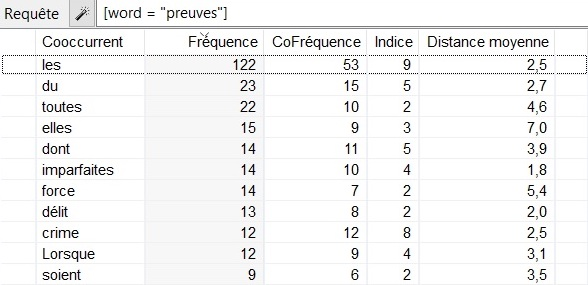
\includegraphics[width=16cm]{Partie3/images/chap3/cooccurrences_preuves.jpg}}
    \caption{Exemple du résultat sur \textsc{txm} des cooccurrences pour le mot \textit{preuves} dans le chapitre 7/13/14 dans les éditions françaises}
    \label{fig:cooccurrences_preuves}
\end{figure}
Nous avons donc, dans cette figure, un tableau de données alors que \textsc{rstudio}, tout comme pour la table lexicale, fournit ces résultats sous la forme d'un graphique, comme illustré par la figure \ref{fig:graphe_chap31}, ce qui présente des avantages et des inconvénients.
\begin{figure}[p]
    %\centering
    \fbox{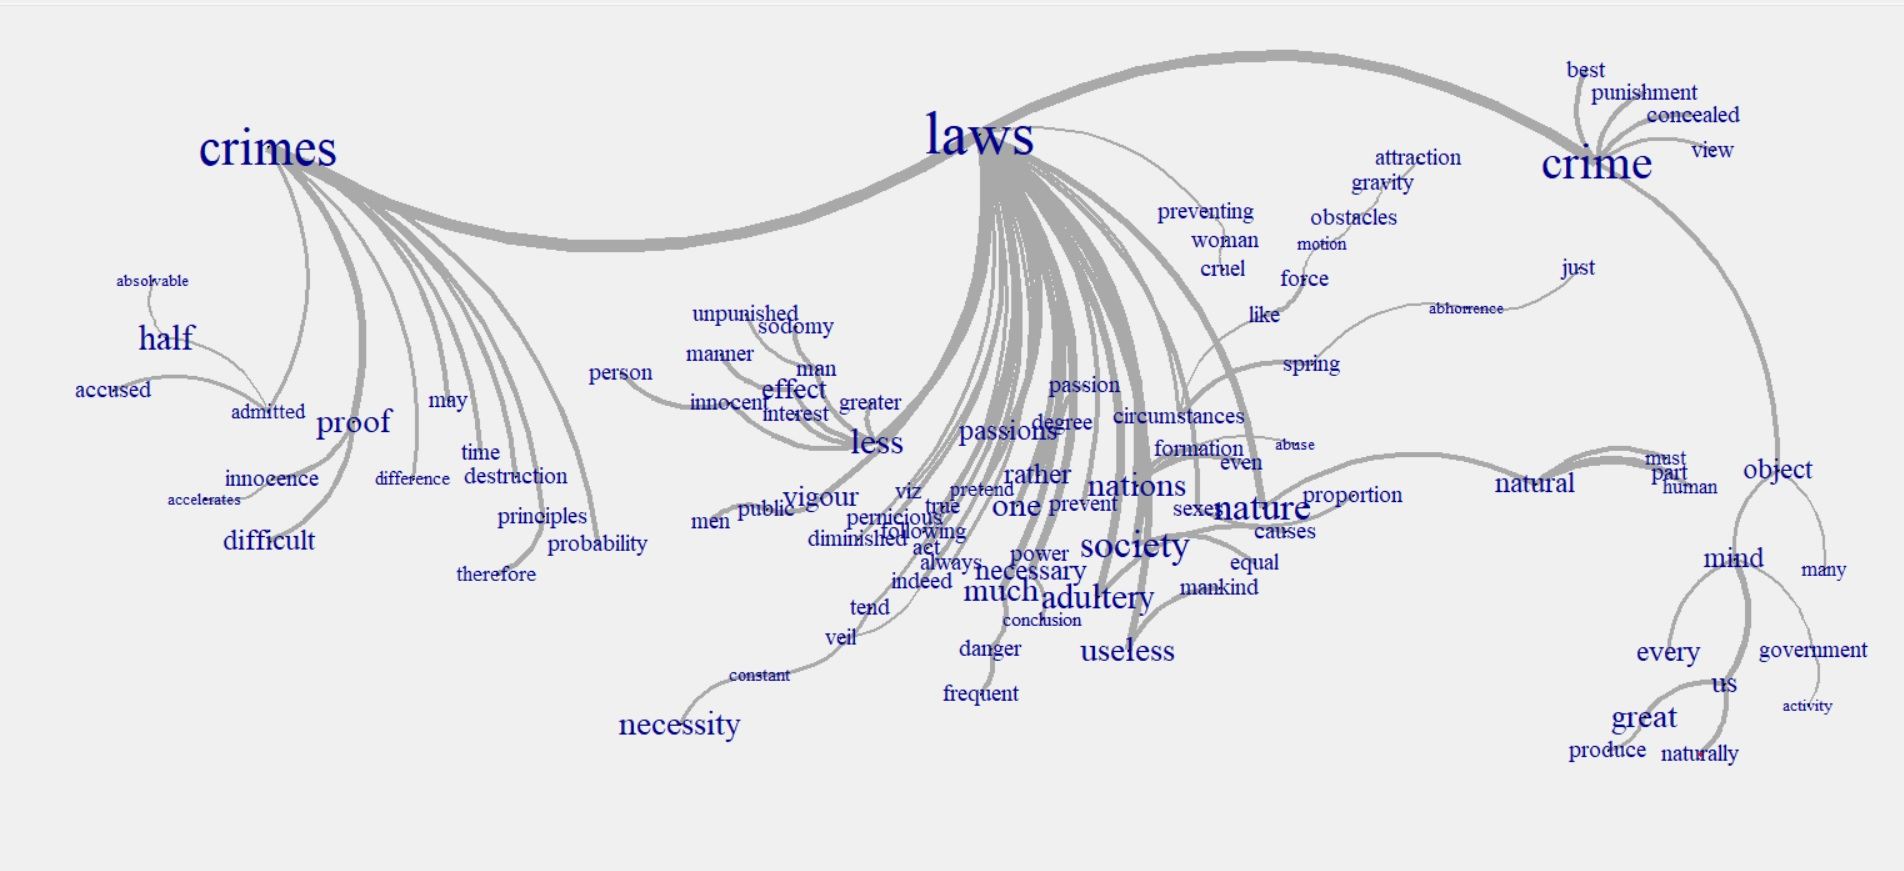
\includegraphics[width=16cm, height=10cm]{Partie3/images/chap3/graphe_chap31.jpg}}
    \caption{Graphe de mots produit par \textsc{r} représentant les cooccurrences dans le chapitre 31 des éditions anglaises}
    \label{fig:graphe_chap31}
\end{figure}
Ce graphe de mots fournit une représentation graphique de notre recherche, ce qui permet d'avoir beaucoup plus de clarté qu'avec la liste qui est produite par \textsc{txm} et de plus, les mots sont de taille différente, tout comme avec le nuage, concédant donc une véritable distinction. Cependant, ce graphe semble prendre en compte absolument tous les mots du corpus qui ne sont pas des mots-vides et donc la clarté disparaît quelque peu, comme cela s'observe pour le mot \textit{laws} dans la figure. Le mot est relié à de nombreuses autres formes mais il devient très difficile de discerner auxquelles. De manière différente, le logiciel \textsc{txm} nous indique la structure de la phrase dans son ensemble plus que ses liens entre les éléments majeurs du lexique. L'articulation entre les deux méthodes sera alors nécessaire puisque \textsc{txm} pourra compléter ce que l'aspect visuel de \textsc{rstudio} semble nous faire perdre, c'est-à-dire les données statistiques\index{Statistique textuelle} qui permettent de véritablement comprendre les liens entre les mots. Pour compléter le graphe, le principe sera donc d'aller y chercher les mots de taille assez importante et de les rechercher dans une requête \textsc{txm} pour obtenir leurs statistiques et donc avoir les chiffres exacts définissant leurs cooccurrences. En ne prenant pas en compte les mots-vides dans le tableau de résultats de \textsc{txm}, nous pouvons donc voir que les cinq co-fréquences les plus fortes avec \textit{laws} sont \textit{crime} (25), \textit{nations} (15), \textit{act} (10), \textit{pernicious} (10) et \textit{prevent} (10). Nous retrouvons ces mots dans le graphe, ce qui montre donc que les deux outils s'articulent effectivement bien ensemble. De plus, cela nous indique différents sens de l'utilisation de \textit{loi} puisque le mot semble principalement lié au terme de \textit{crime}, ce qui a du sens dans le cas du chapitre que nous étudions. Nous pouvons également observer d'autres sens, tel qu'une idée d'empêcher par les lois (\textit{prevent}) ou de les définir comme des lois d'état (\textit{nations}). \pagebreak

Il est possible d'étendre encore plus ces résultats à l'aide des concordances, que nous utiliserons plus en détails dans le chapitre suivant, concordances que nous retrouvons pour les deux logiciels mais qui seront plus claires avec \textsc{txm}. \textsc{txm} donne ici la possibilité d'envoyer les résultats de co-fréquences dans les concordances pour ainsi observer dans quelles parties du texte se placent le bout de phrases contenant les deux termes, comme cela peut se voir avec la figure \ref{fig:concordances_laws_crime}. Cette recherche de co-fréquences permet de développer notre réflexion précédente puisque nous pouvons voir que certains mots s'articulent ensemble telle une expression, comme \og~laws to prevent this crime~\fg{}. D'autres n'ont finalement pas autant de lien que la co-fréquence semblait le montrer, comme cela est représenté avec le premier résultat de la figure \ref{fig:concordances_laws_crime}. \textit{Laws} n'a aucun vrai lien avec \textit{crime}, juste une proximité entre deux phrases. 
\begin{figure}[H]
    \centering
    \fbox{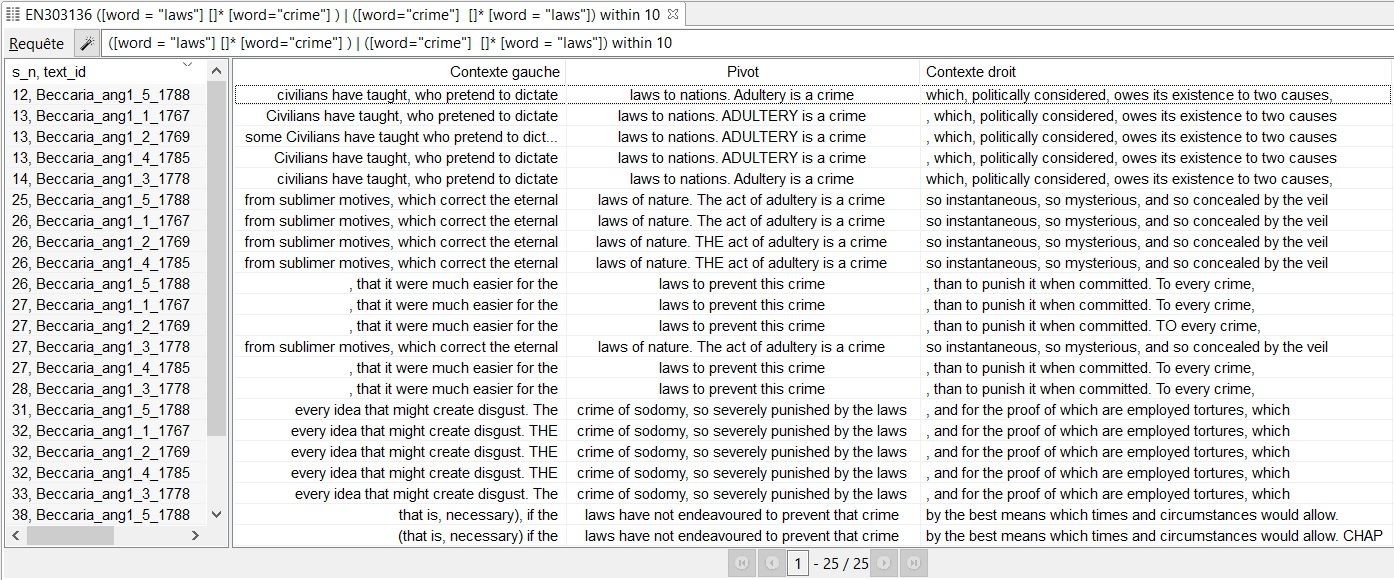
\includegraphics[width=16cm, height=9cm]{Partie3/images/chap3/concordances_laws_crime.jpg}}
    \caption{Résultats de concordances pour la recherche de cooccurrence entre \textit{crime} et \textit{laws} pour le chapitre 31 des éditions anglaises}
    \label{fig:concordances_laws_crime}
\end{figure}

\subsection{Travailler les relations à travers les correspondances~: un corpus qui ne s'approprie pas la méthode}
\textsc{txm} et \textsc{rstudio} disposent également d'autres outils pour présenter les liens du lexique, que nous appellerons ici des correspondances et que nous pourrons observer à travers une fonctionnalité~: l'\acrlong{afc}. C'est un élément très répandu en analyse statistique des données textuelles\index{Statistique textuelle} mais, comme nous le verrons, il ne sera pas adapté à notre corpus et ne donnera pas de résultats fructueux pour notre analyse. \pagebreak

Une \acrfull{afc} permet de 
\begin{quotation}
 \og~structurer l'ensemble des mots en fonction de leur répartition dans les unités textuelles. La représentation des résultats sous forme de graphique [\dots] permet de visualiser la proximité des mots, les oppositions, les tendances\footcite[p.~19]{stat_text_garnier}~\fg{}.
\end{quotation}
 L'intérêt sera donc d'observer des cooccurrences de mots et de mettre en évidence des thèmes et des oppositions de thèmes. Deux éléments de notre corpus justifient le fait que cet outil n'est pas adapté pour notre analyse. Tout d'abord, le corpus n'est pas assez long pour faire ressortir des données utiles. Même si le corpus est composé d'un certain nombre de textes, ces textes ne font chacun qu'environ quatre à six pages, ce qui ne permet pas une étude avancée et la répétition du vocabulaire apporte donc un lexique trop limité pour que cela soit intéressant. Ensuite, la spécificité même du corpus, qui est une répétition du même texte à chaque fois, avec seulement des changements mineurs, indique que cela ne sera pas productif. Le thème sera le même puisque le lexique est, comme nous l'avons vu, très juridique et les changements d'écriture d'un mot n'apporteront que des différences minimes.
\begin{figure}[p]
    \centering
    \fbox{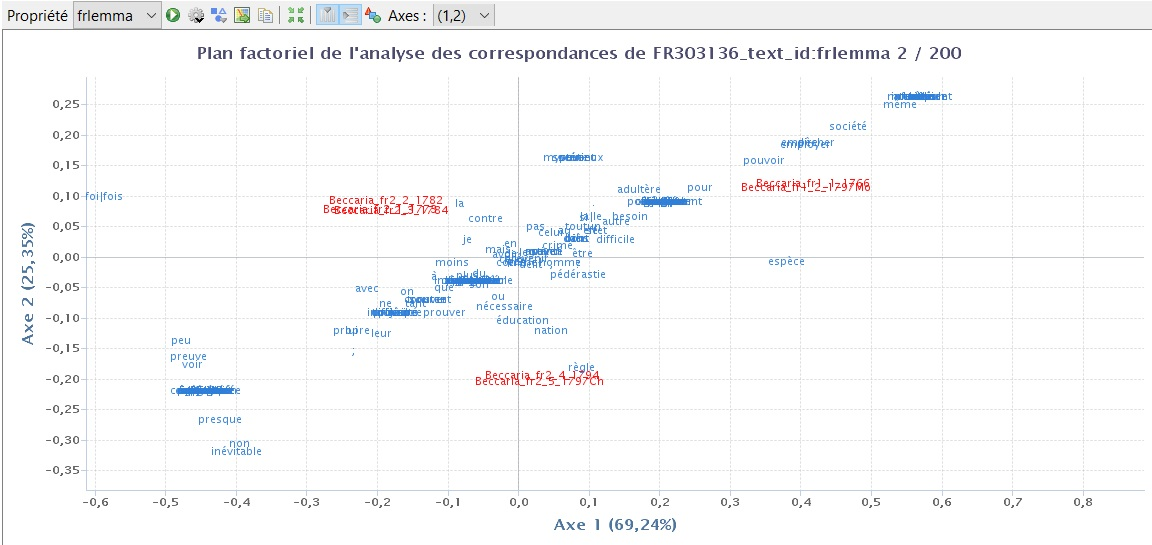
\includegraphics[width=16cm, height=10cm]{Partie3/images/chap3/afc_fr.jpg}}
    \caption{\acrshort{afc} pour le chapitre 30/31/36 des éditions françaises en prenant comme propriété le lemme}
    \label{fig:afc_fr}
\end{figure}
\begin{figure}[p]
    \centering
    \fbox{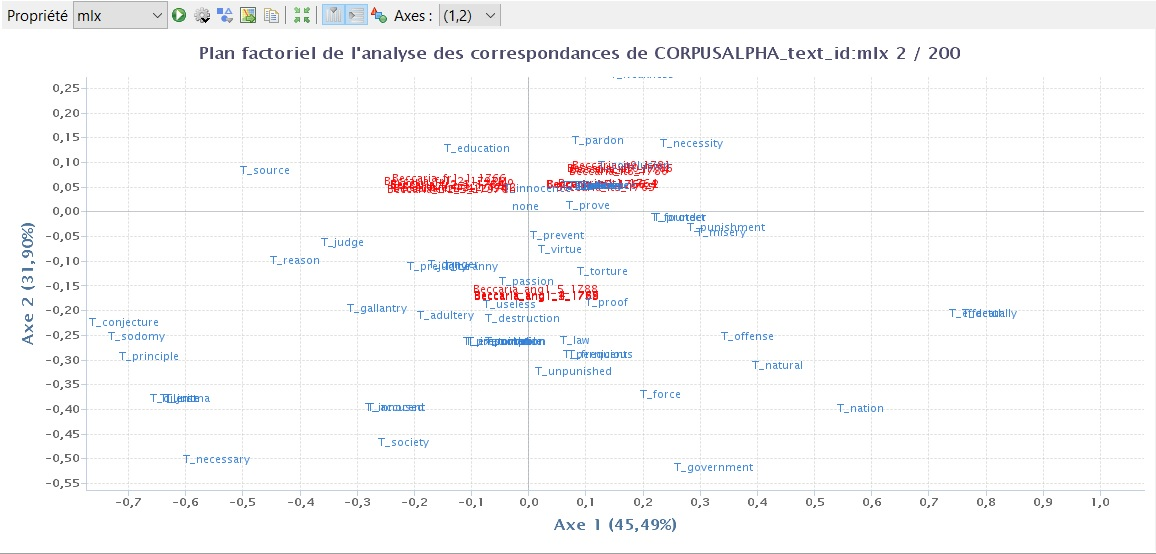
\includegraphics[width=16cm, height=10cm]{Partie3/images/chap3/afc_mlx.jpg}}
    \caption{\acrshort{afc} pour le corpus multilingue\index{Alignement!corpus multilingue} avec comme propriété l'identifiant par termes (mlx)}
    \label{fig:afc_mlx}
\end{figure}
Nous pouvons démontrer ce que nous venons d'expliquer par le biais de deux figures qui présentent deux \acrshort{afc} pour deux types d'analyse du corpus. La figure \ref{fig:afc_fr} montre une \acrshort{afc} pour le chapitre 30/31/36 des éditions françaises avec comme propriété le \textbf{frlemma} tandis que la figure \ref{fig:afc_mlx} montre le corpus multilingue\index{Alignement!corpus multilingue} avec le \textbf{mlx} en propriété. La figure \ref{fig:afc_mlx} semble de base non adaptée par la séparation observée entre les textes~: il y a trois groupes, qui sont chacun des groupes de langues du corpus. Les correspondances ne semblent pas dues tant à des cooccurrences qu'à une proximité linguistique qui influe sur le graphique. Dans le cas de la figure \ref{fig:afc_fr}, nous pouvons également observer trois groupes de textes, qui font référence aux changements mineurs que nous avons évoqué plus tôt, soit les textes structurés par Morellet\index{Morellet, Andre@Morellet, André}, les textes les plus récents avec l'écriture modernisée et le reste des éditions françaises. Les places des termes dans l'une ou l'autre des \acrshort{afc} ne paraissent pas non plus nous fournir de nouveaux éléments puisque pour discerner des thèmes, cela nécessiterait un semblant d'ordre. Ici, nous remarquons pour la figure \ref{fig:afc_fr} une diagonale formée par les lemmes qui se suivent sans discernement et pour la figure \ref{fig:afc_mlx}, il y a un éclatement de tous les \emph{mlx}, avec seulement deux ou trois groupes parfois, ce qui ne nous apporte aucun élément véritablement concret pour notre analyse.

Ainsi, ces deux exemples permettent de démontrer effectivement que les correspondances ne sont pas un moyen efficace et adapté à notre corpus actuel. Elles pourraient être plus utiles dans un cas où l'examen du texte se fait sur l'ouvrage en entier et non juste sur un chapitre précis, puisqu'il pourrait être possible, dans ce cas-là, de discerner plus de groupes de mots, grâce à un vocabulaire plus étendu et plus fourni. \pagebreak

\paragraph{}Cette exploration du corpus nous permet donc de découvrir qu'il existe de nombreux moyens pour effectuer une analyse statistique des données textuelles\index{Statistique textuelle}. Il existe plusieurs logiciels pour cela, qui disposent chacun de nombreux outils pour mener à bien l'étude selon la forme que nous voulons qu'elle prenne. Chacun de ces logiciels possède des caractéristiques propres qui leur permettent d'être plus efficace dans certains cas et surtout plus adapté aux recherches. Nous avons également pu voir que tous les modes de recherches ne sont pas adaptés en fonction du corpus. Dans notre cas, \textsc{txm} et \textsc{rstudio} présentaient chacun des avantages et des inconvénients en fonction de la recherche effectuée et pour la suite de notre travail, ce sera \textsc{txm} qui présentera la meilleure disposition pour mener à bien l'alignement\index{Alignement}, grâce à une méthode que nous avons, pour l'instant, à peine utilisée mais qui sera essentielle pour notre projet~: le concordancier\index{Concordancier}.  
\chapter{Comparer les éditions et les traductions~: méthodes d'alignement partiel des textes}
\fancyhead[LO, RE]{Méthodes d'alignement partiel des textes}

Nous arrivons ici à l'accomplissement de notre objectif. Avant de spécifier quel type d'alignement\index{Alignement} nous effectuerons, nous expliquerons en quoi consiste cette méthode et les moyens utilisés pour la réaliser. Ensuite, nous présenterons le logiciel avec lequel nous extrairons les informations nécessaires, pour les insérer subséquemment dans des tableaux et enfin, explorer ces données pour en tirer des conclusions.

\section{L'alignement\index{Alignement}~: travail sur l'évolution interne d'un texte}
Pour comparer les éditions et les traductions de notre corpus, nous allons utiliser une méthode~: l'alignement\index{Alignement}. Il est donc nécessaire, avant de passer à la mise en pratique, d'évoquer l'origine de cette méthode et la manière dont elle fonctionne.

\subsection{Un concept à la croisée de deux domaines}
L'alignement\index{Alignement} est un concept qui a été développé pour répondre à une problématique posée par la critique génétique textuelle et la méthode mise en place pour l'effectuer s'inscrit dans le domaine du \acrfull{tal}.

La critique génétique textuelle ou génétique des textes est une discipline littéraire qui est née il y a de nombreuses années, afin d'amener une nouvelle méthode de lecture des textes et notamment des manuscrits. L'objectif est d'analyser l'écriture du texte et sa production et cela suit plusieurs étapes. La première s'étend de la conception de l'œuvre par l'auteur jusqu'à la publication. L'étape suivante prend en compte \og~les interventions de l'auteur sur des éditions successives~: depuis l'édition première dite \textit{princeps}, jusqu'à une édition de référence, dite définitive\footcite[p.~1]{genetique_texte}~\fg{}. Enfin, l'analyse porte sur \og~les variations successives du texte dues soit à des erreurs soit à des initiatives des copistes successifs.\footcite[p.~1]{genetique_texte}~\fg{}. Par cette discipline, il y a une recherche sur un corpus de plusieurs versions d'un texte et \og~les généticiens du texte cherchent à reconstituer la genèse de l'œuvre sous ses différents aspects.\footcite{alignement_bourdaillet}~\fg{}. Afin d'effectuer ces recherches, il est donc essentiel de trouver diverses manières d'analyser le texte pour faire ressortir les éléments voulus et c'est ce à quoi sera utilisé l'alignement\index{Alignement}, qui consiste à rechercher les invariants et les différences entre deux textes.

L'étude de plusieurs textes pour repérer des similitudes ou des différences est un travail ardu et assez précis~; l'effectuer manuellement prendrait un temps considérable et serait très fastidieux. Des moyens de répondre à l'alignement\index{Alignement} informatiquement ont donc été recherchés et c'est ainsi que le concept se lie au \acrshort{tal}. Le \acrshort{tal} est une discipline qui associe linguistes et informaticiens et qui a comme objectif l'automatisation des processus, c'est-à-dire \og~mettre en place une chaîne de traitement permettant, à partir d'un ensemble de données injectées en entrée, d'obtenir un résultat distant en sortie.\footcite[p.~1022]{tal_etude_comparee}~\fg{}. L'intérêt est donc de créer des outils, des logiciels ou des programmes informatiques pour travailler automatiquement sur des données linguistiques. Différents algorithmes ont alors été écrits pour obtenir divers résultats, plus ou moins détaillés, de cet alignement\index{Alignement}, afin de faciliter le travail des linguistes en fonction des sources soumises et du corpus à disposition.

\subsection{Fonctionnement de l'alignement\index{Alignement}~: trouver des méthodes efficaces}
Il est nécessaire de prendre en compte un certain nombre d'éléments pour réaliser correctement l'alignement\index{Alignement} et pour savoir quelles données sont significatives pour le travail fait. 

\subsubsection{Quels types de corpus pour l'alignement\index{Alignement} ?}
Un des aspects importants est le corpus et il est possible de réaliser un alignement\index{Alignement} sur quatre types de corpus. Il y a tout d'abord le corpus monolingue ou unilingue\index{Alignement!corpus monolingue} et le corpus multilingue\index{Alignement!corpus multilingue}, dont dans le deuxième cas, la langue est un élément qui rendra l'alignement\index{Alignement} encore plus ardu. 
Ensuite, pour les cas de corpus multilingue\index{Alignement!corpus multilingue}, il y a soit des corpus parallèles, soit des corpus comparables. Dans le premier cas, les textes seront des traductions mutuelles alors que dans le second, les textes ne sont pas les mêmes mais ils possèdent un vocabulaire identique entre les langues. Au milieu de ces deux corpus, il existe un type de corpus quelque peu intermédiaire~: les corpus parallèles bruités, c'est-à-dire des corpus parallèles mais qui ne respectent pas complètement ses contraintes, par des manques ou des décalages dans les documents\footcite[p.~4-6]{alignement_prochasson}. Notre travail d'alignement\index{Alignement} avec le projet MetaLEX\index{Projet MetaLEX} porte à la fois sur des corpus monolingues\index{Alignement!corpus monolingue} puisqu'il existe plusieurs éditions dans une même langue, mais également sur un corpus multilingue\index{Alignement!corpus multilingue} puisqu'une fois tous ces corpus monolingues\index{Alignement!corpus monolingue} réunis, nous les étudierons tous ensemble. Ces corpus sont principalement des corpus parallèles, puisqu'ils sont fondamentalement les mêmes vis-à-vis du texte~: ici donc, c'est la traduction qui nous intéressera notamment. Cependant, il y a aussi des cas de corpus parallèles bruités, puisque nous avons des modifications de certains éditeurs, ce qui signifie que certains textes ne suivent pas les contraintes du corpus parallèle. Ainsi, nous avons une certaine diversité dans notre corpus, ce qui signifie qu'il faudra correctement choisir notre méthode d'alignement\index{Alignement} pour obtenir des résultats satisfaisants. 

\subsubsection{Quelles bases de comparaisons pour l'alignement\index{Alignement} ?}
L'objectif d'un alignement\index{Alignement} est d'observer deux textes et de les comparer dans leur structure et leur fond. Il est donc essentiel de déterminer ce qui sera recherché pour mettre au point cet alignement\index{Alignement}. 

Il existe trois types de différences entre deux textes~: suppressions, insertions et remplacements. La suppression signifie la disparition d'un mot, d'un morceau, d'une phrase ou d'un bloc au sein d'un texte. L'insertion signifie le rajout d'un de ces éléments. Le remplacement se caractérise par une suppression suivie d'une insertion. Avec l'alignement\index{Alignement} que nous avons choisi, il y a également le cas du déplacement qui est à prendre en compte, c'est-à-dire qu'il y a eu une suppression d'un bloc de texte et une insertion ensuite de ce bloc à une autre position. Dans cet alignement\index{Alignement}, il y aura enfin le cas des invariants, c'est-à-dire que certains blocs de texte n'auront absolument pas été modifiés. Ce type d'alignement\index{Alignement} est pratique puisqu'il prend en compte tous les éléments de changements qu'il peut y avoir eu dans un texte et permet donc d'effectuer une analyse exhaustive. L'algorithme de cet alignement\index{Alignement}, comme nous le retrouvons avec \textsc{medite}, fonctionne de manière à aller traiter le texte, identifier les blocs répétés, identifier les invariants et les déplacements~; puis, une fois que tous ces blocs ont été trouvés, il déduira les blocs non répétés, pour nous fournir toutes les données dont nous avons besoin\footcite{alignement_monolingues_bourdaillet_ganascia}. Cependant, cet alignement\index{Alignement} aura un inconvénient~: il est monolingue\index{Alignement!corpus monolingue}. Il ne sera pas possible d'utiliser cet algorithme pour un corpus multilingue\index{Alignement!corpus multilingue}, puisqu'il considérera qu'il n'y a aucun invariant à moins qu'un mot soit le même entre les deux langues. Il faudra donc trouver un moyen d'effectuer les comparaisons entre des corpus de langues différentes.

Ainsi, parmi les méthodes utilisées pour l'alignement multilingue\index{Alignement!alignement multilingue}, il existe celles des points d'ancrage. Cela revient à trouver des informations entre les corpus qu'il est possible de relier de manière fiable pour réaliser l'alignement\index{Alignement}, puisque les langues entre les textes ne seront pas les mêmes. Il est possible de s'appuyer sur des informations structurelles, telles qu'un titre ou une légende mais aussi sur un lexique, en se basant sur un vocabulaire bilingue\footcite[p.~9-10]{alignement_prochasson}. Par cette méthode, la recherche sera facilitée et il sera plus aisé de se baser sur des éléments familiers pour aligner les textes.

\paragraph{}Depuis l'apparition de l'alignement\index{Alignement} comme méthode de critique génétique des textes, il y a donc eu une quantité d'algorithmes produits et de méthodes développées pour étudier un texte, en fonction des besoins et des éléments à disposition. Nous ne les avons pas tous évoqués mais nous nous sommes plutôt concentrés sur ceux que nous allons utiliser dans notre démonstration, afin de réaliser l'objectif de notre projet. L'intérêt sera d'aligner à la fois les corpus monolingues\index{Alignement!corpus monolingue} et les corpus multilingues\index{Alignement!corpus multilingue} mais surtout de travailler avec une procédure qui sera semi-automatique, afin de toujours répondre à la problématique du \acrshort{tal}.

\section{Sonder notre corpus~: réflexions sur la forme de l’alignement\index{Alignement}}
\subsection{Alignement par unité de texte~: un corpus inadapté}
Avant de pouvoir réaliser un quelconque alignement\index{Alignement}, il est nécessaire de délimiter les règles que nous allons suivre pour créer cet alignement\index{Alignement}. Il est capital tout d’abord de sélectionner l’unité de base avec laquelle nous ferons notre analyse. Un alignement\index{Alignement} basique se ferait selon la phrase ou le paragraphe pour un récit ou la ligne dans le cas, par exemple, d’un poème. Cela fut une des propositions avancées pour notre alignement\index{Alignement}, de rechercher les différences de phrases entre nos diverses éditions. Cela posait cependant deux problèmes. Tout d’abord, pour les cas où il y avait eu une restructuration du texte, la phrase aurait essentiellement été modifiée et l’alignement\index{Alignement} deviendrait alors plus compliqué puisqu’il ne serait pas aisé de trouver les limites de la phrase, surtout si elles ont disparu. Ensuite, l’aspect multilingue est problématique vis-à-vis de cet alignement\index{Alignement}. Il peut être difficile de trouver les équivalents de la phrase entre les versions, les différences de ponctuations peuvent influer et en substance, aligner toute une phrase d’une langue à l’autre serait un travail complètement manuel, alors que nous recherchons une méthode semi-automatique pour réaliser cet alignement\index{Alignement}. Cela avait été prouvé par \textsc{medite} qui n’a absolument pas la capacité dans son algorithme de travailler sur deux textes s’ils n’ont pas la même langue. Il ne sera donc pas possible de choisir une unité de texte comme seule base de l’alignement\index{Alignement}.

\subsection{Alignement partiel\index{Alignement!alignement partiel} ciblé\index{Alignement!alignement cible@alignement ciblé}~: une solution d’harmonie avec le projet principal}
La réflexion a donc porté ensuite sur l’idée d’un alignement partiel\index{Alignement!alignement partiel}, qui ne prend en compte qu’un certain type d’éléments pour observer les différences entre les éditions. La détermination de ces éléments s’est rapidement faite, puisque nous avons réfléchi à l’objectif du projet MetaLEX\index{Projet MetaLEX} qui est d’étudier l’évolution des langues historiques du droit en Europe et nous avons donc choisi de réaliser un alignement partiel\index{Alignement!alignement partiel} ciblé\index{Alignement!alignement cible@alignement ciblé} à partir d’un lexique juridique. Le lexique juridique a été établi par les linguistes du projet en suivant le chapitre que nous analysons en priorité et si cette technique d’alignement\index{Alignement} fonctionne, la suite consistera à élargir cette liste afin d’avoir un lexique juridique déterminé avec lequel nous réaliserons la démarche sur l’ensemble de l’ouvrage. Nous avons pu examiner ce lexique juridique dans le chapitre \ref{chap_annotations}, lorsque nous avons mis en place les annotations. Ces dernières seront essentielles à notre travail puisque c’est grâce à elles que nous aurons la possibilité de faire notre alignement\index{Alignement} semi automatiquement mais aussi suivant un corpus multilingue\index{Alignement!corpus multilingue}, où elles représenteront nos points d’ancrage. En travaillant l’alignement\index{Alignement} suivant un lexique, il suffit simplement de trouver les traductions littérales des termes entre les langues et ensuite le travail se fait plus aisément à travers l’identifiant que nous avons apposé plus tôt. Le principe donc de notre alignement\index{Alignement} sera de rechercher les termes juridiques dans les textes à partir d’un identifiant, de trouver les contextes identiques de présence du mot et d’inscrire ces informations dans un tableau de données.

Ce choix du lexique par les identifiants présente tout de même une limite puisque pour sélectionner l’annotation, nous avons réduit le mot à son lemme et cela vaut pour toutes les catégories grammaticales. Ainsi, lorsque l’on relèvera le terme dans notre alignement\index{Alignement}, nous ne prendrons pas en compte les différences au sein même du terme, c’est-à-dire par exemple que nous ne mentionnerons pas le cas où la forme désuète du mot s’est modernisée dans une version plus récente, comme nous l’aurons notamment avec le terme \textit{loi} en français. Cela représente un choix que nous avons fait avec l’alignement\index{Alignement} actuellement réalisé mais cela pourra être rectifié par la suite, lors de l’amélioration du tableau d’alignement\index{Alignement!tableau d'alignement}.

\paragraph{} Ainsi donc, nous avons décidé de ne pas suivre les exemples standards d’alignement\index{Alignement} que nous avons pu présenter dans la première section et nous n’aurons donc pas recours à un des algorithmes qui permettent d’effectuer ces calculs de différences entre plusieurs éditions. Pour réaliser notre alignement\index{Alignement}, nous allons nous appuyer sur le lexique juridique précédemment établi, sur la structure des phrases par le biais d’une numérotation et sur une des fonctionnalités proposées par \textsc{txm}.

\section{Étudier le contexte textuel du lexique juridique~: extraction de données à partir d’un concordancier\index{Concordancier}}
Parmi les outils de statistiques textuelles\index{Statistique textuelle} que nous avons mentionnés et utilisés précédemment, nous avons brièvement évoqué le concordancier\index{Concordancier}. Cet outil permet, pour un mot choisi, de connaître son contexte dans le texte, c’est-à-dire de découvrir les morceaux de phrases qui l’entourent. Cela est fourni dans la majorité des logiciels de textométrie\index{Textometrie@Textométrie} et de lexicométrie et notamment dans les deux auxquels nous avons eu recours. \textsc{rstudio} donne la possibilité, par des lignes de script, de demander les concordances pour un mot donné et il fournit ensuite dans la console les extraits de texte où se trouve ce mot. La méthode fournie par \textsc{txm} est beaucoup plus élaborée et apporte des précisions qui seront primordiales pour notre travail.

\subsection{Le concordancier\index{Concordancier} de TXM~: un outil adapté pour l’alignement\index{Alignement}}
L’interface graphique de \textsc{txm} permet de présenter les résultats du concordancier\index{Concordancier} d’une manière beaucoup plus précise que ne le faisait \textsc{rstudio} et cela nous permet également de mener à bien notre objectif. Elle offre un certain nombre de paramètres qui permettent une précision dans la recherche et avec les résultats, nous observons le pivot, c’est-à-dire le mot que nous avons recherché, son contexte gauche et son contexte droit, ainsi que sa référence. Il est possible également de classer selon ces paramètres, si le choix est plutôt d’étudier par texte ou de voir préférablement le résultat d’un côté de la phrase ou de l’autre, mais également de les modifier selon notre volonté, comme cela est illustré avec la figure \ref{fig:concordancier_parametres}. \textsc{txm} offre ainsi la possibilité de modifier leur forme d’apparition~: les contextes et le pivot sont présentés sous leur forme classique, celle du mot, mais il serait également possible d’avoir le lemme, la catégorie lexicale ou même le \emph{mlx}, que nous avons inséré, pour le pivot, ce qui ne nous montrerait plus les différentes orthographes du mot. De plus, nous pouvons choisir la quantité d’éléments que nous voulons voir apparaître dans ces contextes, pour les cas par exemple où il faut plus de données dans la phrase pour réellement en comprendre le sens. L’un des champs modifiables les plus intéressants dans le cas de notre recherche sera celui des \textbf{Références}. Ce dernier ressort toutes les identifications que fournit \textsc{txm} lorsqu’il encode les textes que nous lui fournissons et il donnera donc la possibilité de faire apparaître les différentes formes du pivot, de mettre la date ou la langue du texte mais il peut aussi fournir des éléments beaucoup plus importants tels que les identifiants du texte ou les numéros de phrases. \textbf{Références} donne enfin la possibilité avec ces paramètres de choisir l’ordre d’apparition dans le tableau des résultats et de choisir les clés et l’ordre de tri. Ainsi, il sera possible de faire apparaître la phrase selon un ordre alphabétique des mots de chacun des contextes ou il sera possible de sélectionner comme référence le numéro de phrase et l’identifiant de textes et c’est ce que nous allons privilégier dans notre travail, en les classant dans cet ordre pour faciliter notre alignement\index{Alignement}.
\begin{figure}[H]
    \centering
    \caption{Paramètres de commande pour une requête de concordance sur \textsc{txm}}
    \fbox{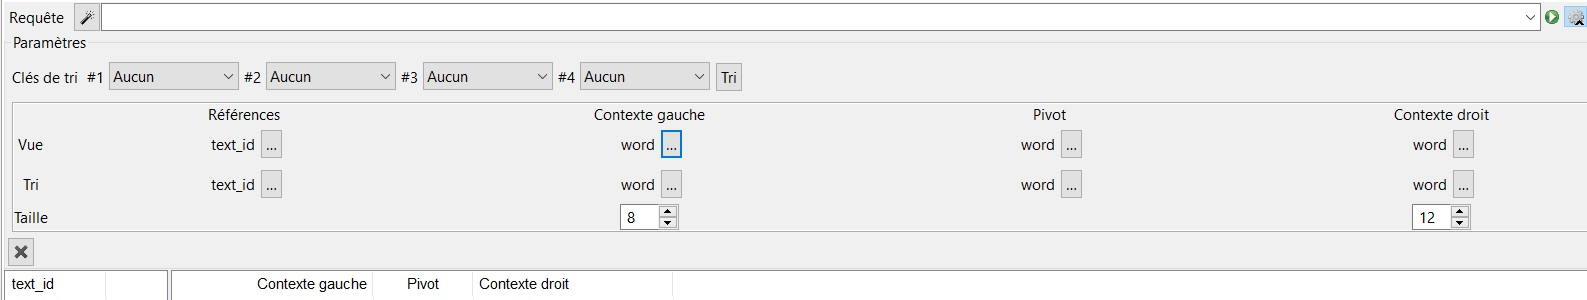
\includegraphics[width=16cm, height=3.5cm]{Partie3/images/chap4/concordancier_parametres.jpg}}
    \label{fig:concordancier_parametres}
\end{figure}

\subsection{Exemple d’une requête tirée du lexique}
Afin d’illustrer l’intérêt du concordancier\index{Concordancier} pour la réalisation de notre alignement\index{Alignement}, le meilleur moyen est de fournir un exemple à partir du corpus multilingue\index{Alignement!corpus multilingue} qui a été annoté avec les termes du lexique juridique et qui a ensuite été importé sur le logiciel sous le nom de CORPUSALPHA. Nous choisissons pour l’exemple un terme monolexical pour les trois langues~: \og~T\_adultery~\fg{}. Nous avons choisi comme clé de tri le numéro de phrase et l’identifiant de texte et nous avons effectué un classement dans l’ordre croissant pour l’un puis chronologique pour l’autre. 
\begin{figure}[p]
    \centering
    \fbox{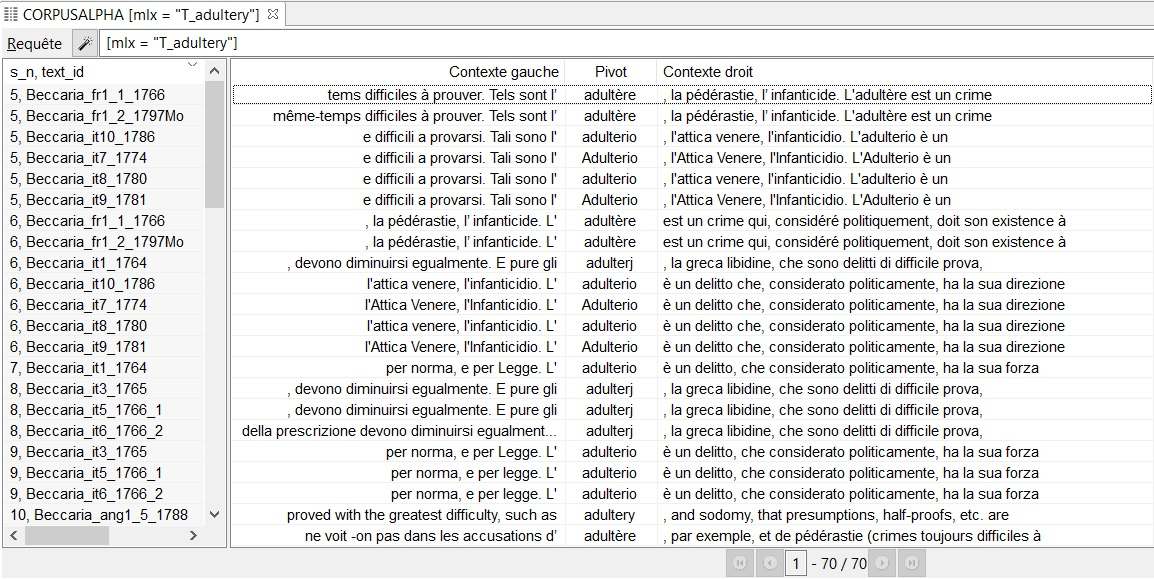
\includegraphics[width=17cm, height=10cm]{Partie3/images/chap4/concordancier_adultery.jpg}}
    \caption{Recherche de concordances pour l’identifiant \og~T\_adultery~\fg{} à travers le corpus multilingue CORPUSALPHA}
    \label{fig:concordancier_adultery}
\end{figure}
Nous pouvons donc observer avec cette requête, illustrée avec la figure \ref{fig:concordancier_adultery}, plusieurs éléments. Tout d’abord, nous pouvons voir que la forme \textit{adultère} a été annotée 70 fois avec l’identifiant. Le mot apparaît également ici dans toutes les langues donc il n’y a pas eu d’erreur d’annotation pour l'une d'elles, comme nous en avons eu à quelques reprises qui ont pu fausser l’alignement\index{Alignement}. Nous pouvons également observer qu’avec l’identifiant, les différences de formes ou de présentation du mot ne comptent pas, comme la majuscule par exemple. Ensuite, nous pouvons constater, dans la colonne des \textbf{Références}, que le classement par numéro de phrase a effectué un mélange de langues entre les éditions, ce qui peut illustrer le fait que même les différences de langues n’ont pas influé sur la structure de la phrase pour certaines éditions. Enfin, avec ce classement, on peut déjà reconnaître quelle phrase sera alignée avec une autre grâce au contexte, puisque l’on retrouve des phrases d’une même langue qui sont identiques, mais également entre deux langues. Il est déjà possible d’affirmer, par exemple, juste en observant la figure que certaines phrases en français et en italien seront sur la même ligne du tableau\index{Alignement!tableau d'alignement}, en observant simplement leur contexte droit~:
\begin{itemize}
    \item \og~adultère [\dots] considéré politiquement~\fg{} (fr)
    \item \og~adulterio [\dots] considerato politicamente~\fg{} (it)
\end{itemize}
En suivant ces traductions plus ou moins littérales, nous aurons ainsi la possibilité d’établir notre alignement\index{Alignement} de la manière la plus complète possible, puisque le concordancier\index{Concordancier} permet en plus de pallier certains obstacles que nous avons évoqués précédemment.

\subsection{\label{section_resolution}Une résolution partielle de certaines limites de l’alignement\index{Alignement}}
Les différentes options d’affichage du concordancier\index{Concordancier} donnent la possibilité de pousser notre travail un peu plus loin qu’en faisant simplement apparaître les expressions monolexicales puisqu’elles vont nous permettre de ne pas limiter l’alignement\index{Alignement} à ces expressions. Le concordancier\index{Concordancier} nous offre également l’opportunité de corriger les cas où certains mots n’ont pas été annotés car ils n’étaient pas reconnaissables par le script Python dans le dictionnaire qui avait été soumis. Ces deux solutions s’articuleront dans certains cas afin de parfaire notre alignement\index{Alignement}.

Dans le chapitre \ref{chap_annotations}, nous avions présenté un obstacle inhérent à la liste de termes juridiques et au balisage du texte que nous annotions~: lorsque certains termes sont polylexicaux, il n’est pas possible d’annoter comme nous avions pu le faire pour les expressions monolexicales. Nous avions alors proposé une solution un peu limitée, qui consistait à annoter un seul mot de l’expression, proposition que nous avions ensuite rejetée car cela serait trop compliqué de retrouver le reste de l’expression. Cette limite disparaît à partir du moment où nous travaillons avec le concordancier\index{Concordancier}. Comme nous l’avons expliqué, le concordancier\index{Concordancier} de \textsc{txm} permet de faire apparaître les contextes droit et gauche de la phrase dont est tirée la forme annotée. Ainsi, à partir du moment où nous avons connaissance de l’expression exacte que nous recherchons, il est possible, lors de l’apparition des résultats du mot annoté, de distinguer les phrases et expressions qui correspondent à ce que nous avons dans notre lexique juridique et ainsi de rajouter les expressions polylexicales dans notre alignement\index{Alignement}.
\begin{figure}[p]
    \centering
    \fbox{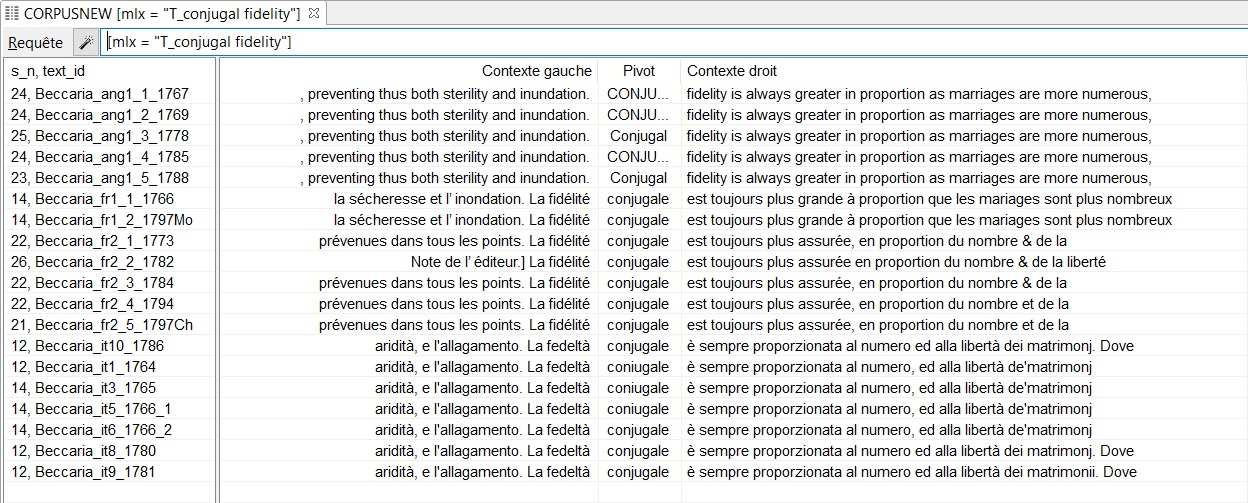
\includegraphics[width=17cm, height=10cm]{Partie3/images/chap4/concordancier_conjugal_fidelity.jpg}}
    \caption{Recherche de concordances pour l’identifiant \og~T\_conjugal fidelity~\fg{} à travers le corpus multilingue\index{Alignement!corpus multilingue} CORPUSALPHA}
    \label{fig:concordancier_conjugal_fidelity}
\end{figure}

L’exemple que nous avons avec la figure \ref{fig:concordancier_conjugal_fidelity} est celui de l’expression de \textit{fidélité conjugale}, significative dans le cas de ce chapitre spécifique et en deux mots, ce qui oblige à un choix d’annotation. J’ai choisi ici d’annoter le terme \textit{conjugal} plutôt que \textit{fidélité} puisque j’ai considéré qu’il était possible que le terme de fidélité se retrouve autrement dans le texte, si nous prenons en compte le fait que le chapitre débat de l’adultère, alors qu’il était plus probable que l’adjectif \textit{conjugal} ne se retrouve que lié à la fidélité. L’intérêt particulier de cette annotation est l’identifiant que nous lui avons donné. J’ai annoté la forme \textit{conjugal} avec l’expression complète de \textit{fidélité conjugale}. Cela signifie que, dans le cas où la forme se trouve sous un autre contexte dans le texte, il faudra chercher le terme \textit{fidélité} dans les contextes qui l’entourent pour s’assurer de faire correctement l’alignement\index{Alignement} et de choisir les bons éléments. De ce fait, cette méthode accroît la source d’annotations qui nous permettra de réaliser le tableau d’alignement\index{Alignement!tableau d'alignement}. Cela n’est cependant pas complètement efficient, puisqu’il existe certaines expressions qui sont composées d’autres expressions annotées ou qui sont trop compliquées pour faciliter l’encodage et cela obligera alors à effectuer un travail un peu plus manuel pour trouver les éléments manquants.

Nous devrons alors effectuer également une recherche plus ou moins manuelle pour contourner l’autre limite. Pour réaliser l’annotation, nous avons rédigé un script informatique, que nous avons associé à un dictionnaire de termes juridiques et que nous avons appliqué au texte que nous avons ensuite importé dans le logiciel \textsc{txm}. Toute cette démarche est majoritairement automatique, tout comme la recherche d’une expression clé avec le concordancier\index{Concordancier} ensuite, ce qui nous permet d’avoir accès à un grand nombre de mots rapidement et facilement. Pour rechercher les termes qui n’ont pas été correctement annotés, nous procédons à un travail bien plus manuel puisque nous devons aller observer le contenu de l’édition pour trouver la forme du terme dans un des textes spécifiques d’une édition pour pouvoir le rechercher ensuite dans le concordancier\index{Concordancier} et trouver les informations dont nous avons besoin pour l’alignement\index{Alignement}. Par cette technique, nous pourrons ainsi aller chercher les cas où les annotations n’ont pas fonctionné. Nous pouvons citer comme exemple \textit{half-proof}/\textit{half proof} en anglais qui pose plusieurs difficultés. L’écriture n’est pas la même entre les versions, puisqu’elle prend parfois un tiret. Le terme \textit{proof} a déjà été identifié dans le texte et la forme \textit{half} est utilisée à plusieurs reprises. L’identifiant avec un seul terme n’est donc pas ici possible et cette technique manuelle sera la seule productive pour ce cas-là.

\paragraph{}Le concordancier\index{Concordancier} de \textsc{txm} offre ainsi de nombreuses fonctionnalités qui nous permettront d’extraire une grande quantité de données profitables à notre travail afin d’aller dans les détails et de fournir un tableau d’alignement\index{Alignement!tableau d'alignement}, qui sera le plus complet possible.

\section{Mettre en forme les données recueillies~: réalisation de tableaux d’alignement\index{Alignement!tableau d'alignement}}
À l’aide de toutes les informations que nous avons recueillies lors du travail sur \textsc{txm}, nous avons la possibilité d’établir un alignement\index{Alignement} sous la forme d’un tableau\index{Alignement!tableau d'alignement}, dont nous présenterons tout d’abord une version simple, puis une version avancée plus détaillée.

\subsection{Transcrire les informations extraites~: établissement du tableau d’alignement\index{Alignement!tableau d'alignement} simple}
Dans un premier temps, nous avons décidé d’établir un tableau d’alignement\index{Alignement!tableau d'alignement} simple, qui rapporte les numéros de phrases où se trouve l’expression choisie dans le texte, en fonction des éditions, et les cas où elle n’y est pas. Le tableau\index{Alignement!tableau d'alignement} porte sur le chapitre 30/31/36 et se compose de colonnes qui comprennent toutes les éditions que nous avions dans notre étude du concordancier\index{Concordancier} et de lignes qui contiennent les termes juridiques, avec plusieurs lignes pour un même terme dans les cas où ce dernier apparaît plusieurs fois dans le texte. 

L’intérêt est alors de récupérer dans le concordancier\index{Concordancier} les différentes phrases où apparaît le terme choisi, de chercher les similitudes entre deux éditions, de la même langue ou d’une langue différente. Dans les cas où il y a des utilisations identiques du terme, nous inscrivons dans le tableau d’alignement\index{Alignement!tableau d'alignement}, les numéros de phrases selon ce qui a été établi par \textsc{txm}. Sur la même ligne, se trouvera le numéro de phrase pour chacune des éditions qui utilise le terme dans le même contexte. 

Il existe cependant des cas où une édition n’apparaît pas dans les résultats du concordancier\index{Concordancier}. Nous vérifions alors que ce terme n’a pas été mal inscrit, selon la méthode manuelle évoquée dans la section précédente. Dans les cas où cela est avéré, nous cherchons son numéro de phrase, pour l’inscrire dans le tableau\index{Alignement!tableau d'alignement}. Dans les cas où il n’y a pas eu d’erreur et où le terme ne figure effectivement pas, nous inscrivons un signe pour signifier l’absence du terme (un \emph{slash} dans le cas de notre tableau\index{Alignement!tableau d'alignement}). 

Nous pouvons en observer un échantillon dans le tableau\index{Alignement!tableau d'alignement} \ref{table:alignement_simple}, avec l’exemple du terme \textit{preuve}, identifié par l’annotation \og~T\_proof~\fg{}.
Le tableau\index{Alignement!tableau d'alignement} nous permet de voir que le terme \textit{preuve} apparaît de huit manières différentes au sein de toutes les éditions et qu’il y a des cas où cette utilisation est commune à toutes les versions ou presque et d’autres cas où cela représente une spécificité d’une édition ou même d’une langue en particulier. Ainsi, par exemple, avec ce terme là, nous pouvons voir que l’édition française de 1782 emploie le terme identifié par \og~T\_proof~\fg{} d’une manière qui n’est reprise par aucun autre texte. La dernière ligne de la figure permet de constater qu’il y a également un cas où seules les éditions anglaises utilisent le terme. 

Par ailleurs, nous pouvons remarquer qu’il y a de nombreuses situations où le terme n’aura pas été utilisé, sans autre explication dans le tableau\index{Alignement!tableau d'alignement}. C’est ce détail qui sera ajouté dans le nouveau tableau\index{Alignement!tableau d'alignement} plus précis et plus développé de notre alignement\index{Alignement}.

\subsection{Consigner les modifications effectuées~: enrichissement avec le tableau d’alignement\index{Alignement!tableau d'alignement} avancé}
Dans un second temps et afin de parfaire notre travail, nous avons décidé de rajouter de nouveaux éléments dans le tableau\index{Alignement!tableau d'alignement} ayant pour objectif d’apporter les informations que nous n’avions pas dans le premier tableau\index{Alignement!tableau d'alignement}, c’est-à-dire remplacer tous les \textit{slashs} qui signalaient une non-présence du terme juridique et indiquer ce qu’il y a à la place. En observant les différentes éditions et en recherchant les zones de textes où le terme juridique aurait dû apparaître, nous avons pu distinguer différents types de changements que nous avons classé en quatre catégories~:
\begin{itemize}
    \item R = Remplacement~: le terme a été remplacé par un autre mot~;
    \item S = Suppression~: le terme a été supprimé dans cette version du texte et n’existe plus~;
    \item I = Inexistant~: le contexte du terme est inexistant dans une édition~;
    \item E = Équivalent~: le terme a changé mais la racine est la même.
\end{itemize}
En plus de ces différentes informations, nous rajoutons deux autres détails pour compléter notre tableau d’alignement\index{Alignement!tableau d'alignement}. Dans les cas d’une suppression ou d’une inexistence du terme, nous mettons simplement l’identifiant de la catégorie. Dans les cas d’un remplacement ou d’une équivalence, nous allons spécifier le numéro de phrase du nouveau terme, afin de savoir si, bien qu’il y ait un changement, la structure et le contexte de la phrase n’ont pas changé. Puis nous renseignons le terme qui structure la phrase à la place de celui que nous recherchons.

Dans le but d’observer cela, nous pouvons reprendre l’exemple que nous avions présenté dans la première sous-section, avec cette fois-ci les éléments qui composent le tableau d’alignement\index{Alignement!tableau d'alignement} avancé, ce que nous observons avec le tableau\index{Alignement!tableau d'alignement} \ref{table:alignement_avance}.
En reprenant les observations de la première sous-section, nous pouvons donc y ajouter des éléments. L’édition française de 1782 semblait avoir une utilisation unique du terme choisi et après recherche dans les différents textes, nous pouvons effectivement voir que cela est dû à une note de bas de page dans l’édition, ce qui explique que la catégorisation pour le reste de la ligne sera \og~inexistant~\fg{}. Nous pouvons observer également des cas d’équivalences, avec la septième utilisation de \og~T\_proof~\fg{} dans le texte, où cela est équivalent avec \textit{semi-preuves} ou \textit{half-proof}. Nous voyons ici le cas que nous avions évoqué dans la sous-section \ref{section_resolution}, où le tiret changeait l’encodage du mot et donc l’annotation subséquente. Ici donc, nous avons une équivalence, puisque le terme \textit{preuve} est utilisé mais avec un élément supplémentaire. Cet exemple nous permet également d’observer des cas de suppressions de l’utilisation du mot, ainsi que des remplacements, où le terme de \textit{preuve} ne convenait pas et où il y a un nouveau terme, qui est cependant à la même place que l’est \textit{preuve} dans les autres contextes. Nous pouvons distinguer, avec la troisième apparition de \og~T\_proof~\fg{} que les éditions utilisent le même terme en lieu et place de \textit{preuve}~: \textit{produce}. Cela peut indiquer une considération des traducteurs pour mieux retranscrire l’idée générale de la phrase.

\paragraph{}Ainsi donc, avec ces différents tableaux, nous discernons des cas où l’alignement\index{Alignement} n’est pas parfait puisque le terme utilisé est le même mais il n’est pas présent dans les mêmes phrases mais aussi des cas où nous avons un alignement\index{Alignement} entre les phrases mais où le terme utilisé n’est pas identique. Les tableaux produits fournissent déjà, de ce fait, un certain nombre d’informations sur les éditions, sur leurs similitudes et leurs différences mais il sera nécessaire de les étudier plus en profondeur pour en tirer véritablement des réponses.

\begin{landscape}
\pagestyle{empty}
\begin{table}
\centering
\caption{Échantillon du tableau d’alignement simple avec l’identifiant \og~T\_proof~\fg{}}
\begin{longtable}{|c|c|c|c|c|c|c|c|c|c|c|c|}
\hline

 & fr2\_2 & fr2\_3 & fr2\_4 & fr2\_7 & ang1\_1 & ang1\_2 & ang1\_3 & ang1\_4 & ang1\_5 & it1 & it3 \\
 & 1782 & 1784 & 1794 & 1797 & 1767 & 1769 & 1778 & 1785 & 1788 & 1764 & 1765 \\ \hline
T\_proof & / & / & / & / & / & / & / & / & / & 1 & 3 \\ \hline
T\_proof & 5 & 5 & 5 & 4 & 4 & 4 & 4 & 4 & 3 & 1 & 3 \\ \hline
T\_proof & / & / & / & / & / & / & / & / & / & 5 & 7 \\ \hline
T\_proof & 9 & 9 & 9 & 8 & / & / & / & / & / & / & / \\ \hline
T\_proof & 10 & 10 & 10 & 9 & 9 & 9 & 10 & 9 & 8 & / & / \\ \hline
T\_proof & 22 & / & / & / & / & / & / & / & / & / & / \\ \hline
T\_proof & / & / & / & / & 11 & 11 & / & 11 & / & 6 & 8 \\ \hline
T\_proof & / & / & / & / & 32 & 32 & 33 & 32 & 31 & / & / \\ \hline

\end{longtable}
\label{table:alignement_simple}
\end{table}
\begin{table}
\caption{Échantillon du tableau d’alignement avancé avec l’identifiant \og~T\_proof~\fg{}}
\begin{longtable}{|c|c|c|c|c|c|c|c|c|c|c|c|}
\hline

 & fr2\_2 & fr2\_3 & fr2\_4 & fr2\_7 & ang1\_1 & ang1\_2 & ang1\_3 & ang1\_4 & ang1\_5 & it1 & it3 \\
 & 1782 & 1784 & 1794 & 1797 & 1767 & 1769 & 1778 & 1785 & 1788 & 1764 & 1765 \\ \hline
T\_proof & 3\_E & 3\_E & 3\_E & 2\_E & 3 & 3 & 3 & 3 & 2 & 1 & 3 \\
 & T\_prove & T\_prove & T\_prove & T\_prove &  &  &  &  &  &  &  \\ \hline
T\_proof & 5 & 5 & 5 & 4 & 4 & 4 & 4 & 4 & 3 & 1 & 3 \\ \hline
T\_proof & 9 & 9 & 9 & 8 & 8\_R & 8\_R & 9\_R & 8\_R & 7\_R & 4\_R & 6\_R \\
 &  &  &  &  & produce & produce & produce & produce & produce & T\_prove & T\_prove \\ \hline
T\_proof & 10 & 10 & 10 & 9 & 9 & 9 & 10 & 9 & 8 & 5\_R & 7\_R \\
 &  &  &  &  &  &  &  &  &  & T\_prove & T\_prove \\ \hline
T\_proof & S & S & S & S & S & S & S & S & S & 5 & 7 \\ \hline
T\_proof & 22 & I & I & I & I & I & I & I & I & I & I \\ \hline
T\_proof & 11\_E & 11\_E & 11\_E & 11\_E & 11 & 11 & 12\_E & 11 & 10\_E & 6 & 8 \\
 & sémi-preuves & sémi-preuves & semi-preuves & sémi-preuves &  &  & half-proofs &  & half-proofs &  &  \\ \hline
T\_proof & 34\_R & 28\_R & 28\_R & 27\_R & 32 & 32 & 33 & 32 & 31 & S & S \\
 & soupçon & soupçon & soupçon & soupçon &  &  &  &  &  &  &  \\ \hline
 
\end{longtable}
\label{table:alignement_avance}
\end{table}
\end{landscape}

\section{Relever les données~: exploration du tableau\index{Alignement!tableau d'alignement} produit}
Après avoir réaliser notre alignement partiel\index{Alignement!alignement partiel} selon un lexique de termes juridiques, la finalité consiste à exploiter ces tableaux et à relever des informations qui mettent en avant l’intérêt de l’alignement\index{Alignement}, mais aussi des éléments qui doivent être expliqués.

\subsection{Différence de numérotations~: entre changements internes et anomalie logicielle}
En étudiant les échantillons des tableaux d’alignement\index{Alignement!tableau d'alignement} \ref{table:alignement_simple} et \ref{table:alignement_avance}, nous pouvons prêter attention aux numéros des phrases, à leurs similitudes et à leurs divergences. Nous pouvons voir tout d’abord qu’il y a des cas où la numérotation est la même, comme pour les éditions françaises de 1773, 1782, 1784 et 1794. À un certain point du texte, l’édition de 1782 voit sa numérotation diverger avec les autres. Les éditions françaises de l’abbé Morellet\index{Morellet, Andre@Morellet, André} ont la même numérotation sur tout le texte. Enfin, l’édition de Chaillou de Lisy\index{Chaillou de Lisy, Etienne} de 1797 a un décalage d’une phrase de moins avec les autres éditions du même traducteur. La première partie des éditions italiennes (1764 à 1766) a la même numérotation, excepté la toute première qui semble avoir deux phrases de moins que le reste des textes ayant la même structure en italien. La deuxième partie des éditions italiennes, qui suivent la nouvelle structure de l’abbé Morellet\index{Morellet, Andre@Morellet, André} (1774 à 1786) ont, de même, une numérotation identique à travers tout le texte. Enfin les éditions anglaises ont de légères différences de numérotation. Trois des éditions ont exactement la même numérotation du début à la fin du texte et deux éditions ne sont décalées que d’une phrase, une de plus pour 1778 et une de moins pour 1788. 

Ces différences peuvent s’expliquer par deux raisons dont la première est entièrement liée à notre sujet de travail, c’est-à-dire les changements internes dus aux modifications faites par les traducteurs. Ainsi, le texte de l’édition française de 1782 a une numérotation qui change à cause de diverses notes de bas de page rajoutées par son traducteur. Les textes structurés par Beccaria\index{Beccaria, marquis de} et ceux structurés par Morellet\index{Morellet, Andre@Morellet, André} ont également un alignement\index{Alignement} qui diverge, ce qui est dû à une différence dans la composition des textes. Outre ces différences dues à notre critique propre, il y a une autre raison, qui s’explique par le travail de \textsc{txm}. Le logiciel a réalisé l’encodage lorsque nous lui avons soumis le corpus plus tôt dans notre démarche et il a donc effectué une séparation par phrase dont son critère de fin est le point. Cela présente quelques difficultés qui influent sur la numérotation des phrases et de ce fait, sur l’alignement\index{Alignement}. Nous avons décidé lors du traitement du texte (dans le chapitre \ref{chap_mise_en_forme}) de laisser la ponctuation comme elle était inscrite dans le manuscrit. Cela donne lieu à des légères différences qui se démarquent dans l’alignement\index{Alignement}. Le début d’un chapitre commence par l’annonce d’un chapitre, son numéro, le titre et ensuite le chapitre commence. Traditionnellement, dans les textes que nous avons à disposition, chacune de ces parties est séparée par un point, ce qui signifie une phrase pour chaque selon \textsc{txm}. Cependant, il existe un cas en anglais (ang1-5 1788) ainsi qu’un en français (fr2-7 1797) où entre le mot \textit{chapitre} et le numéro, il n’y a aucun point. Ce détail décale donc toute la numérotation et présente des différences dans l’alignement\index{Alignement}, dont il faut tenir compte tout en prenant en considération la raison, à savoir la ponctuation choisie par les traducteurs. La toute première édition italienne (it1) présente également une particularité dans sa numérotation, puisque dans la première publication du marquis de Beccaria\index{Beccaria, marquis de}, les numéros de chapitre n’étaient pas indiqués et seuls les titres de chapitres figuraient en début de paragraphe. Cela supprime donc deux phrases, selon la logique du logiciel \textsc{txm} et décale l’édition italienne de 1764 par rapport aux suivantes. Ce détail représente une fusion de nos deux raisons, puisque si effectivement le texte ne change pas dans le fond, un choix avait été fait au début de ne pas mettre de numérotation de chapitre. 

La numérotation est ainsi un élément majeur à considérer dans le cas d’un alignement\index{Alignement}, puisqu’elle informe déjà sur la composition du texte, sur les modifications qui ont été effectuées par les traducteurs et cela nous fournit donc un nombre de données dans notre critique génétique du texte. L’autre élément qu’il faut alors observer est l’ampleur des similitudes d’utilisation du terme et des changements quand il n’y a pas alignement\index{Alignement}.

\subsection{Exploration de l’alignement\index{Alignement}~: quelques particularités du tableau\index{Alignement!tableau d'alignement}}
Nous n’avons rempli qu’une fraction du tableau d’alignement\index{Alignement!tableau d'alignement} du chapitre 30/31/36, en ne sélectionnant que quelques termes juridiques pour vérifier la démarche et illustrer notre objectif. Parmi les termes juridiques de la liste, nous avons recherché \textit{preuve}, \textit{adultère}, \textit{loi}, \textit{infamie}, \textit{peine}, \textit{vérité}, \textit{torture}, p\textit{uissance paternelle}, \textit{infanticide}, \textit{pédérastie} et \textit{crime}. Nous avons donc choisi des termes assez génériques pour notre \emph{Traité\index{Traite des delits et des peines@Traité des délits et des peines}}, ainsi que des termes essentiels pour le chapitre étudié. Leur étude permet déjà de faire apparaître, grâce à l’alignement\index{Alignement} avancé, des éléments qui illustrent l’intérêt de notre travail. 

Nous pouvons tout d’abord observer, en reprenant notre exemple précédent, que la forme \textit{preuve} a parfois été remplacée et, comme évoqué dans le chapitre \ref{chap_annotations}, les traducteurs ont, à plusieurs reprises, effectué une verbalisation du mot, ce qui signifie qu’à la place d’une forme qui sera identifiée par \og~T\_proof~\fg{}, nous aurons une identification \og~T\_prove~\fg{}. Cela se retrouve également à d’autres endroits du texte pour l’italien et le français, où il est nécessaire cette fois-ci d’avoir une réflexion inversée, puisque l’utilisation du verbe avait été faite dans les premières éditions de Beccaria\index{Beccaria, marquis de}, ce qui indique donc que les traducteurs ont considéré que l’utilisation du nom apporterait une meilleure compréhension dans la démonstration qui est faite. Cela établit le concept d’une interprétation de l’éditeur lors de la traduction, pour trouver la meilleure façon de retranscrire ces idées.

Nous remarquons une autre modification dans le texte qui représente pour ce cas précis un changement de l’idée que Beccaria\index{Beccaria, marquis de} cherche à exprimer. Deux termes juridiques peuvent s’articuler dans notre démarche~: \og~T\_paternal\_authority~\fg{} et \og~T\_tyranny~\fg{}. Le premier n’apparaît qu’une seule fois dans le chapitre, alors que le second apparaît deux fois. L’une des apparitions de \og~T\_tyranny~\fg{} est cependant assez éphémère avant d’être remplacée par l’autre terme, \og~T\_paternal\_authority~\fg{}. En effet, dans son chapitre sur \og~Des délits difficiles à prouver~\fg{}, Beccaria\index{Beccaria, marquis de} traite de fidélité conjugale et de la liberté du mariage. Dans ses deux premières publications en 1764 et 1765, Beccaria\index{Beccaria, marquis de} mentionne que la \textit{tyrannie} génère ou défait les mariages. Lors de ses corrections publiées dans les éditions de 1766, ce terme change pour devenir une action faite par la \textit{puissance paternelle}. Il y a donc là un changement dans la composition même du texte, non pas par les éditeurs mais par l’auteur même. Nous pouvons donc dire avec cet exemple que l’auteur semble avoir voulu atténuer son propos, tout en apportant une précision.

Parmi les autres cas particuliers, il y a ceux où les changements paraissent être dus à une limite du vocabulaire entre les langues. Nous pouvons retrouver de nombreuses utilisations du terme \og~T\_loi~\fg{}, omniprésent en raison du sujet même de la source. Il y a cependant des emplois du mot qui ne sont valables que pour une des langues par manque d’un autre terme possible. Ainsi, dans deux cas, les éditions françaises et italiennes mentionnent la \textit{législation/legislatrice} et le \textit{législateur/legislatore}. Le lexique juridique anglais ne parait toutefois pas posséder d’équivalent et les traducteurs adoptent le terme de \textit{laws} pour véhiculer l’idée du texte. Il sera alors nécessaire d’étudier le contexte de la phrase pour déterminer si le sens de la démonstration en est affecté. Parmi nos termes, nous retrouvons un autre cas similaire dans les éditions anglaises, ainsi qu’italiennes, avec le terme de \textit{crime}. Dans les versions françaises, deux termes sont utilisés pour mentionner des actes répréhensibles~: \textit{délit} et \textit{crime}. Ils indiquent aujourd’hui une différence de gravité de l’acte mais à l’époque, les deux mots semblaient être plutôt considérés comme des synonymes. Cette nuance n’existe pas ou peu pour les deux autres langues. En anglais, seul \og~T\_crime~\fg{} est utilisé tout au long du texte pour désigner et l’un et l’autre. En italien, il y a bien une exception où c’est le mot \textit{reato}, signifiant littéralement crime, qui est utilisé~; pendant tout le reste de la démonstration, l’auteur, puis les traducteurs utilisent systématiquement le terme de \textit{délit}. Cette particularité nous permet de constater que ce sont les traducteurs français qui ont décidé d’indiquer une nuance dans le texte, en utilisant les deux termes. De plus, en examinant le tableau d’alignement\index{Alignement!tableau d'alignement}, nous remarquons qu’il existe des cas où les versions de Morellet\index{Morellet, Andre@Morellet, André} et de Chaillou de Lisy\index{Chaillou de Lisy, Etienne} ne sont pas semblables et où l’un a préféré \textit{crime} là où l’autre a transposé \textit{délit} mais en majorité, le choix de l’un ou l’autre des termes a été le même. Cela peut indiquer un sens commun du texte pour ces deux traducteurs, mais également une approbation du second pour certains choix de traductions effectués par le premier.

L’observation du tableau d’alignement\index{Alignement!tableau d'alignement} avancé nous apporte donc déjà un certain nombre de détails sur les changements qui ont été effectués dans le texte soit par l’auteur, soit par les éditeurs et traducteurs. Les informations recueillies portent sur des différences par langue, des vocabulaires plus ou moins limités ou encore une volonté d’être plus compréhensible, autant de cas justifiant l’intérêt de la réalisation d’un tableau d’alignement\index{Alignement!tableau d'alignement} sur un corpus multilingue\index{Alignement!corpus multilingue}.

\paragraph{} Ainsi, à l’aide d’un bon logiciel de statistiques textuelles\index{Statistique textuelle} et d’une idée bien définie du contenu de l’alignement\index{Alignement}, il est possible d’atteindre notre objectif final, tel qu’il a été déterminé au terme de notre démarche~: un alignement semi-automatique, partiel\index{Alignement!alignement partiel} et ciblé\index{Alignement!alignement cible@alignement ciblé} à partir d’un lexique juridique. Par le biais de nombreuses et diverses opérations, nous obtenons assez de matière pour mettre en forme un maximum de données afin de réaliser la critique génétique du texte et alors, d’étudier notre source de la manière la plus approfondie possible, pour en extraire les évolutions et modifications du vocabulaire juridique.

\part*{Conclusion}
\addcontentsline{toc}{part}{Conclusion}
\fancyhead[LO, RE]{Conclusion}

\paragraph{} L'alignement\index{Alignement} est un procédé encore en développement qui peut prendre plusieurs formes et se baser sur des textes variés. Il peut être nécessaire de trouver une méthode propre pour l'effectuer, selon nos besoins, ce que nous avons finalement accompli. Au fur et à mesure du stage, nous avons procédé à de nombreuses opérations afin de travailler le texte et d'en ressortir divers éléments et données. Cela nous a permis principalement de mettre en place une démarche afin d'accomplir l'objectif du stage~: un alignement partiel\index{Alignement!alignement partiel}, ciblé\index{Alignement!alignement cible@alignement ciblé} à partir d'un lexique juridique. Nous avons donc maintenant à notre disposition un processus, partant d'un manuscrit numérisé, forme de base de notre corpus, et arrivant à un tableau d'alignement\index{Alignement!tableau d'alignement}, simple ou avancé, finalité de notre stage, qui peut être représenté à l'aide du schéma suivant.
\begin{figure}[H]
    \centering
    \fbox{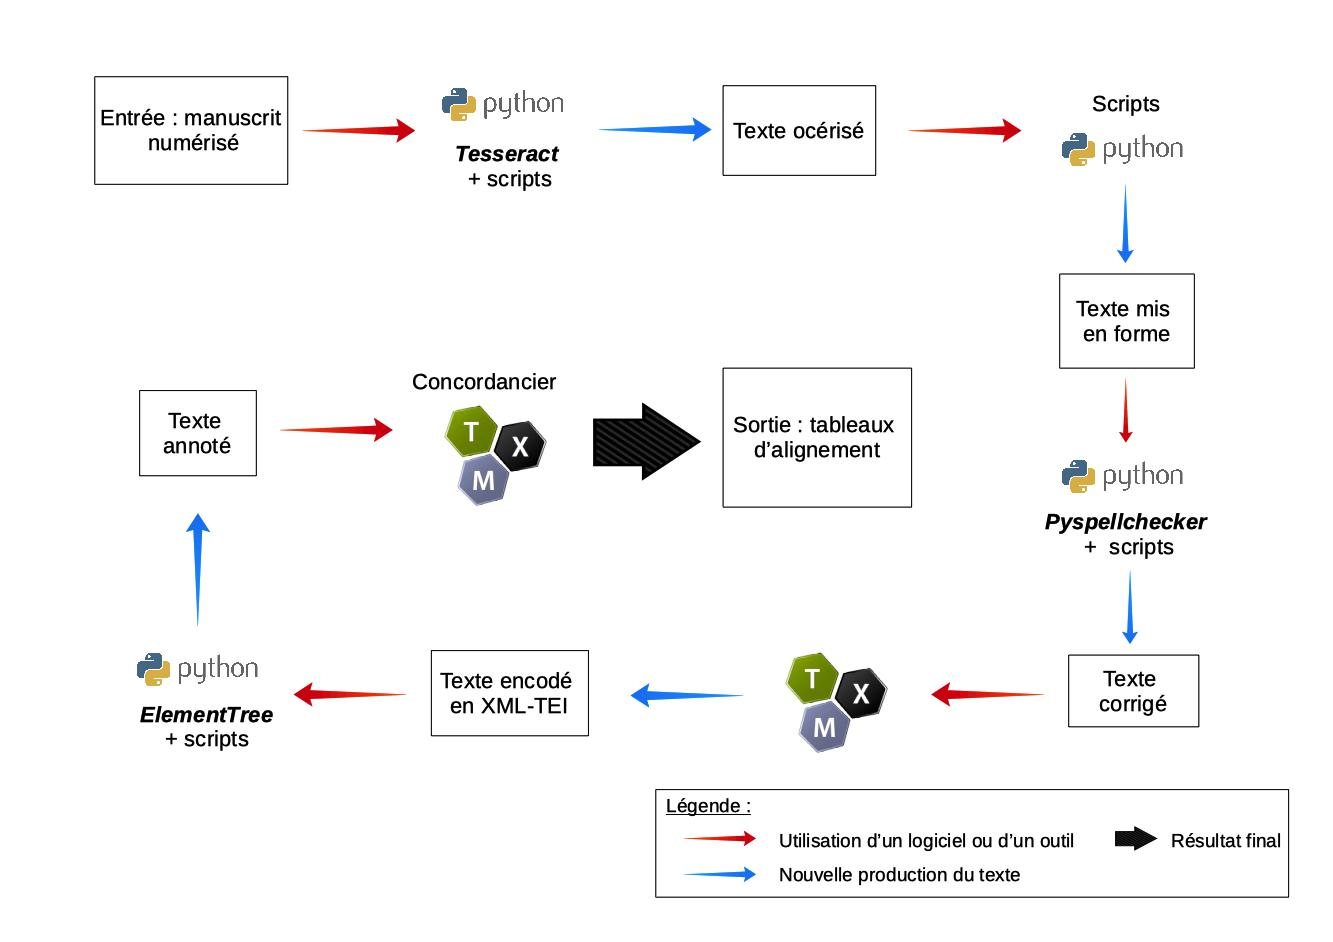
\includegraphics[width=16cm]{Conclusion/processus_pour_alignement.jpg}}
    \caption{Processus représentant la démarche pour effectuer l'alignement\index{Alignement}}
    \label{fig:processus_alignement}
\end{figure}
Nous partons ainsi de notre fichier de base et à chaque utilisation d'un nouveau logiciel, d'un nouvel outil et/ou de l'exécution d'un script Python, nous obtenons une nouvelle forme du texte, texte qui évolue progressivement, afin d'atteindre une forme qui, à l'aide du concordancier\index{Concordancier} de \textsc{txm}, nous permet de rédiger les tableaux d'alignement\index{Alignement!tableau d'alignement}. Nous avons donc un processus ne nécessitant pas une grande quantité d'étapes, impliquant l'installation de quelques logiciels et l'exécution de plusieurs scripts pour produire à la fin un alignement\index{Alignement} devant reposer sur un lexique. 

\paragraph{} Nous avons effectué, en parallèle de notre démarche principale, d'autres opérations sur notre corpus. Certaines de ces opérations étaient requises car elles permettaient de répondre à un des enjeux du stage. Grâce aux analyses textuelles, par la lecture et par quelques outils, nous avons pu établir la généalogie des éditions à disposition. Cette finalité nous a ainsi permis d'obtenir diverses informations sur les éditions en elle-même et non juste sur un chapitre en particulier. Cela a, de plus, aidé au travail futur et à la démarche principale puisque cela a fourni une base de connaissances sur les origines de chacune des éditions. D'autres opérations n'étaient pas obligatoires mais donnaient la possibilité d'approfondir nos connaissances sur le texte, de manière plus générale que l'alignement ciblé\index{Alignement!alignement cible@alignement ciblé} que nous avons effectué et moins limitée par le travail exclusif d'un seul chapitre. Grâce aux statistiques textuelles\index{Statistique textuelle} que nous avons extraites des différents chapitres traités, nous avons pu en apprendre plus sur le lexique, sur la formation des textes, sur leur structure mais aussi sur leurs différences et sur ce qui fait leur particularité. Ces analyses ont offert un point de vue plus général sur les textes que le seul travail basé sur l'aspect juridique qui a conduit à l'alignement\index{Alignement}. Ces opérations parallèles nous ont donc apporté des informations supplémentaires et intéressantes sur notre corpus, sans avoir à être liées exclusivement à l'alignement\index{Alignement}.

\paragraph{} Tout le travail n'a tout de même pas été fait. Si la démarche a commencé à être effectuée avec les éditions allemandes, cela ne représente qu'une petite fraction du travail et l'alignement\index{Alignement} lui-même, élément majeur du projet, n'aura pas été du tout réalisé pour l'allemand, pourtant une des premières langues dans laquelle le corpus a été traduit. Les textes n'ont pas été corrigés, ni importés sur le logiciel et il n'a pas été possible de retravailler la liste de termes juridiques pour rajouter les bons termes en allemand. Sans cela, il n'était pas possible de compléter le travail et cela restera donc une partie importante qui demeure inachevée. Par ailleurs, vers la fin du stage, de nouvelles éditions en français, allemand et italien ont été acquises, soit car il a enfin été possible de les numériser, soit car elles n'ont été découvertes qu'à ce moment, et le temps imparti pendant le stage empêchait de réaliser toute la démarche et de rajouter ces textes dans les analyses effectuées et dans les tableaux d'alignement\index{Alignement!tableau d'alignement}. Cela représente donc à la fois un travail inachevé puisque le corpus était à disposition et une perspective de travail pour la suite.

\paragraph{} Nous avons réalisé notre travail efficacement et sans trop de difficultés mais il s'est tout de même présenté certaines limites. Dans le cadre de l'océrisation\index{OCR!ocerisation@océrisation} de nos textes, nous avons choisi comme logiciel \emph{Tesseract}. Le logiciel fonctionne aisément avec notre corpus mais il est tout de même possible de soulever la problématique de son efficacité dans le cas d'une utilisation plus intensive. Nous n'avons travaillé que sur un à trois chapitres pendant le stage mais dans le cas d'un traitement plus important du corpus, nous pourrions vouloir traduire de plus grands extraits du \emph{Traité}\index{Traite des delits et des peines@Traité des délits et des peines} et un plus grand nombre de chapitres. Dans ce cas-là, \emph{Tesseract} pourrait ne plus être assez productif et efficient pour le projet et il serait nécessaire de changer pour un logiciel d'\acrshort{ocr}\index{OCR} plus avancé. Ensuite, lors de la majeure partie de la démarche pour l'alignement\index{Alignement}, nous avons travaillé avec la plateforme \textsc{txm}. Si elle a montré qu'elle était un outil puissant et très utile, nous avons tout de même relevé une limite. Lors de l'encodage des textes, \textsc{txm} considère le point dans un texte comme le signe d'une fin de phrase, ce qui n'est pas systématiquement le cas. Nous nous sommes cependant basés sur cela pour extraire les numéros de phrase pour l'alignement\index{Alignement}. Si la majeure partie des informations était exacte, nous avons observé qu'il y avait certains cas où la coupure de phrase n'était pas correcte et que le point ne signifiait pas réellement la fin d'une phrase, ce qui influe sur les données des tableaux d'alignement\index{Alignement!tableau d'alignement}. Ainsi, dans ce cas-là, il pourrait être nécessaire de devoir changer la manière dont l'encodage est fait, comme par exemple en effectuant par nous-même la coupure des phrases en utilisant un script qui prend en compte plus de critères que juste un point, tout en pouvant tout de même importer le texte sur \textsc{txm} afin qu'il l'encode comme nous le souhaitons. Nous pourrions aussi trouver un moyen de modifier certains paramètres de \textsc{txm} afin qu'il change ses méthodes d'encodage pour mieux prendre en compte la structure du texte. Enfin, la dernière limite peut porter sur notre travail final~: l'alignement\index{Alignement} semi-automatique. Au regard du travail que nous devons effectuer pour mettre en place les tableaux d'alignement\index{Alignement!tableau d'alignement}, il pourrait être remis en cause le fait qu'il y a trop de travail manuel dans la démarche et que nous pourrions faire plus d'opérations automatiques. Nous réfléchirions alors à l'idée par exemple d'extraire certaines informations du concordancier\index{Concordancier} avec un script plutôt qu'à la main, ce qui pourrait être une nouvelle perspective de travail.

\paragraph{} Au regard de ce que nous avons réalisé dans l'ensemble sur le projet, cela peut s'avérer bénéfique dans le futur. Tout d'abord, nous avons mis en place tout un système partant d'un manuscrit numérisé et non océrisé\index{OCR!ocerisation@océrisation}, pour aller jusqu'à un texte annoté et, encore plus loin, un alignement\index{Alignement}. Nous avons créé de ce fait un schéma et un guide à suivre, non seulement pour le corpus que nous travaillons mais possiblement également pour d'autres textes et ouvrages que des chercheurs voudront travailler de la même manière que notre projet. La disponibilité des scripts mais aussi de leur moyen d'exécution contribue à cette utilisation future. De plus, nous avons articulé un certain nombre de modules, tel que \emph{Tesseract}, \emph{Pyspellchecker} ou \emph{ElementTree}, qui peuvent servir consécutivement à un procédé commun. Nous avons pu également développer certains de ces modules, comme \emph{Pyspellchecker} auquel nous avons rajouté des listes de fréquences pour différentes langues. Notre démarche a pu aussi montrer l'importance de \textsc{txm} pour des travaux à la fois d'analyses, de statistiques textuelles\index{Statistique textuelle} et d'alignements avec divers outils. La multitude de langues qu'il propose pour l'exécution du travail est très bénéfique et nous avons montré qu'il pouvait \oe uvrer aussi bien avec des corpus monolingues\index{Alignement!corpus monolingue} qu'avec des multilingues\index{Alignement!corpus multilingue}. Le travail constant de renouvellement de \textsc{txm}, comme notamment avec l'amélioration de la pratique des annotations, permet d'en faire un outil indispensable à notre démarche, avec lequel nous pourrons rechercher des utilisations plus approfondies.

\paragraph{} Pour finir, nous pouvons réfléchir aux perspectives du projet et aux moyens pour le développer. Tout d'abord, le processus que nous avons mis en place pourra être exécuté pour le reste du corpus. Comme nous l'avons expliqué, toutes les éditions du corpus que nous avons actuellement n'ont pas été traitées et il faudra donc réaliser ce travail. Ce dernier pourra être étendu à plus de chapitres mais aussi à d'autres corpus. Le \emph{Traité des délits et des peines\index{Traite des delits et des peines@Traité des délits et des peines}} a également été traduit en espagnol, dont il existe plusieurs éditions datant d'avant 1800. Cela implique un autre corpus monolingue\index{Alignement!corpus monolingue} qui pourra être traité comme tel pour les analyses et statistiques textuelles\index{Statistique textuelle} et qui pourra également être ajouté au corpus utilisé pour l'alignement\index{Alignement}. La démarche ayant déjà été sollicitée pour trois langues (voire quatre jusqu'à un certain point), son utilisation avec un corpus d'une autre langue pourra renforcer l'intérêt de cette démarche. Il est également possible de réfléchir à d'autres manières d'appréhender l'alignement\index{Alignement} de nos textes, avec le cas par exemple de la présentation par des éditions synoptiques, c'est-à-dire voir toutes les éditions ensemble avec une sélection de bouts de phrase ou de blocs de textes correspondants sur chacune des éditions pour travailler l'alignement\index{Alignement} avec un visuel plus conséquent. Cette perspective, réfléchie avec les responsables de la plateforme \textsc{txm}, entrainerait une modification d'une partie de la démarche (à partir de l'encodage) et une utilisation intensifiée du logiciel avec lequel nous pourrions réaliser l'encodage et l'annotation du texte. Cette nouvelle démarche, bien que très intéressante, porterait cependant moins sur le lexique juridique que celle que nous avons développée, aspect qui reste tout de même essentiel à notre projet.

\appendix
\part*{Annexes}
\addcontentsline{toc}{part}{Annexes}
\chapter{Scripts Python}
\fancyhead[LO, RE]{Scripts Python}

Pendant toute la durée de stage, le travail dépend de la création et de l'exécution de divers scripts utilisant le langage Python. Ces scripts sont présentés et expliqués dans le mémoire à l'aide de diagrammes d'activité et de courts paragraphes, pour illustrer la démarche réalisée. 
Dans cette annexe, chacun des scripts qui a été mentionné dans le mémoire sera nommé et brièvement présenté. Ils seront également rattachés aux figures correspondantes dans le mémoire. Il est possible de retrouver chacun de ces scripts sur le Github de la Plateforme Géomatique, ainsi que la façon dont ils peuvent être executés, dans un repository dédié au projet MetaLEX\index{Projet MetaLEX} : \url{https://github.com/PSIG-EHESS/metalex}

\section{OCR}
\paragraph{ocr\_jpg.py} : Figure \ref{fig:OCR} 

Script d'\acrshort{ocr}\index{OCR} pour les images au format \textsc{jpeg}

\paragraph{ocr\_tiff.py} : Figure \ref{fig:OCR}

Script d'\acrshort{ocr}\index{OCR} pour les images au format \textsc{tiff}

\section{Nettoyage de texte}
\paragraph{1\_mise\_en\_forme.py} : Figure \ref{fig:etape1}

Script qui permet de supprimer les numéros de pages et la ponctuation dans un texte donné, ainsi que changer la mise en forme du texte, pour supprimer les nombreuses mises à la lige tout en conservant les structures de paragraphes

\paragraph{script1.sh} : Script shell pour exécuter le script 1\_mise\_en\_forme.py

\pagebreak

\paragraph{2\_verification\_orthographique.py} : Figure \ref{fig:etape2}

Script qui permet de repérer les mots inconnus dans un fichier donné selon un dictionnaire de langue choisi et qui place ses mots et la correction proposée dans un dictionnaire Python

\paragraph{script2.sh} : Script shell pour exécuter le script 2\_verification\_orthographique.py

\paragraph{3\_mise\_en\_forme\_bis.py} : Figure \ref{fig:etape3}

Script qui permet de supprimer les numéros de pages dans un texte donné, ainsi que changer la mise en forme du texte, pour supprimer les nombreuses mises à la ligne tout en conservant les structures de paragraphes

\paragraph{script3.sh} : Script shell pour exécuter le script 3\_mise\_en\_forme\_bis.py

\paragraph{4\_correction\_orthographique.py} : Figure \ref{fig:etape5}

Script qui permet de remplacer dans un fichier donné les mots erronés relevés par le deuxième script et trié lors du nettoyage du dictionnaire produit. Ces mots sont remplacés par la correction proposée comme valeur de la clé dans le dictionnaire

\paragraph{script4fr.sh} : Script shell qui permet d'exécuter le script 4\_correction\_orthographique.py pour le cas des textes en français

\section{Normalisation}
\paragraph{script\_regex\_normalisation.py} : Figure \ref{fig:normalisation_txm}

Script pour insérer, depuis un dictionnaire importé et dans un fichier \textsc{xml}, une nouvelle balise contenant la forme normalisée du mot, en utilisant les expressions régulières

\paragraph{script\_xml\_normalisation.py} : Figure \ref{fig:normalisation_txm}

Script pour insérer depuis un dictionnaire, importé et dans un fichier \textsc{xml}, une nouvelle balise contenant la forme normalisée du mot, en utilisant un module Python pour le \textsc{xml}

\paragraph{script\_replace.sh} : Script pour exécuter l'un ou l'autre des deux scripts, en fonction du groupe de ligne non mis en commentaire 

\pagebreak

\section{Annotations}
\paragraph{script\_regex\_annotation.py} : Figure \ref{fig:annotation_txm}

Script pour insérer, depuis un dictionnaire importé et dans un fichier \textsc{xml}, une nouvelle balise contenant un identifiant lié à un terme juridique ou une valeur \og none \fg{}, en utilisant les expressions régulières

\paragraph{script\_xml\_annotation.py} : Figure \ref{fig:annotation_xml}

Script pour insérer, depuis un dictionnaire importé et dans un fichier \textsc{xml}, une nouvelle balise contenant un identifiant lié à un terme juridique ou une valeur \og none \fg{},  en utilisant un module Python pour le \textsc{xml}

\paragraph{script\_annotations.sh} : Script pour exécuter l'un ou l'autre des deux scripts, en fonction du groupe de ligne non mis en commentaire
\chapter{Glossaire}
\fancyhead[LO, RE]{Glossaire}

Le glossaire contient les définitions des termes clés de notre projet, notamment un lexique portant sur l'étude statistique de texte, ainsi que certains termes plus obscurs que nous pouvons retrouver dans le corps du texte.

\paragraph{Alignement\index{Alignement}} : Méthode visant à analyser deux ou plusieurs versions d'un même texte pour rechercher les différences et les invariants existants.

\paragraph{Analyse Factorielle des Correspondances (\acrshort{afc})} : Méthode qui permet d'étudier l'association entre deux variables qualitatives. Elle sert à décrire et hiérarchiser des relations statistiques.

\paragraph{Collation} : Comparaison d'exemplaires manuscrits ou imprimés entre eux.

\paragraph{Concordancier} : Logiciel qui travaille des chaînes de caractères au sein d'un texte et permet de placer, pour toutes ses occurences, un mot recherché dans le contexte droit et gauche de la phrase où il se trouve.

\paragraph{Cooccurrence} : Présence simultannée de mots ou groupes de mots dans un même extrait de taille restreinte.

\paragraph{\og Débruitage \fg{}} : Élimination du \og bruit \fg{} dans une image numérisée, c'est-à-dire éliminer les pixels noirs qui se sont rajoutés dans les zones de pixels blancs, ce qui peut engendrer une déformation de certains caractères ou des éléments dans les zones de lecture qui perturbent la reconnaissance de caractères. Ce bruit peut avoir pour origine un problème lors de la numérisation ou être dû à l'état de la page du manuscrit, qui peut avoir des ratures ou des détériorations.

\paragraph{Géomatique} : Ensemble des outils et méthodes permettant d'acquérir, de représenter, d'analyser et d'intégrer des données géographiques. 

\paragraph{Lemmatisation} : Identification d'un mot sous sa forme canonique (le lemme représente le singulier d'un nom, le masculin singulier d'un adjectif, l'infinitif d'un verbe, etc.).

\paragraph{Lexicométrie} : Science linguistique étudiant statistiquement l'utilisation des mots.

\paragraph{Métalexicographie} : Discipline qui étudie les méthodes et les principes guidant la création des dictionnaires.

\paragraph{Reconnaissance Optique de Caractères (en anglais, Optical Character Recognitition (\acrshort{ocr}))\index{OCR}} : Procédé permettant de transformer les images d'un texte, dactylographié ou manuscrit, en des fichiers électroniques au format texte.

\paragraph{Statistique textuelle\index{Statistique textuelle}} : Outil mêlant à la fois statistique classique, linguistique, analyse du discours et informatique, qui permet d'étudier des textes en utilisant les méthodes statistiques.

\paragraph{Textométrie\index{Textometrie@Textométrie}} : Discipline développée principalement dans les années 1970 qui se base sur les méthodes d'analyse des données appliquées à des données linguistiques et textuelles. Elle met en avant des modèles statistiques qui rendent compte de caractères significatifs de texte : attirances contextuelles des mots, linéarité et organisation interne du texte, contrastes intertextuels ou indicateurs d'évolution lexicale. La textométrie\index{Textometrie@Textométrie} met donc en avant un large éventail de calculs et de statistiques pour analyser des collections de textes.

\paragraph{Traitement Automatique des Langues (\acrshort{tal})}: Discipline qui associe linguistes et informaticiens. Son objectif est de développer des logiciels ou programmes informatiques capables de traiter automatiquement des données linguistiques, en prenant en compte les spécificités du langage humain. Les principaux domaines sont le traitement de la parole, la traduction automatique, la compréhension automatique des textes, la gestion électronique de l'information et des documents existants et la génération automatique de textes.
\chapter{Outils et programmes}
\fancyhead[LO, RE]{Outils et programmes}

Le travail effectué pendant le stage a requis l'utilisation de nombreux logiciels, outils, modules et programmes pour la réalisation des étapes du projet. Dans cette annexe, nous présentons ces éléments, suivant une classification thématique, en fournissant le lien URL vers lequel il est possible de trouver de plus amples explications, ainsi qu'une définition rapide et une description de son fonctionnement.

\section{Général}
\paragraph{ElementTree} : \url{https://docs.python.org/fr/3/library/xml.etree.elementtree.html}

Module Python qui donne la possibilité d'analyser et de créer des données pour du \textsc{xml}. Il s'utilise par le biais de deux éléments : \textit{ElementTree} et \textit{Element}. \textit{ElementTree} représente le fichier \textsc{xml} comme un arbre et \textit{Element} représente un nœud dans l'arbre. À l'aide de diverses fonctions et de plusieurs classes d'objets, il est possible de rechercher des informations dans l'arbre \textsc{xml}, d'effectuer des modifications dans le contenu de cet arbre ou même de créer, à partir de rien, un arbre \textsc{xml} avec des balises, des attributs et des valeurs.

\paragraph{Github} : \url{https://github.com/}

Github est une plateforme web de versionnage et de collaboration qui permet notamment de développer des logiciels et autres applications. Elle donne la possibilité de versionner son code source et les différents avancées de son travail, en gardant l'historique de tous les changements faits. Elle permet la collaboration entre développeurs à l'aide d'outil tel que \textit{issues} ou \textit{pull request} qui permet de prendre en compte les améliorations ou modifications que pourraient proposer d'autres personnes et de les ajouter à son code source. Le travail est collaboratif aussi grâce à l'aide de branches et de \textit{merge} qui permet de travailler sur des bouts de code et de rajouter cela au projet principal (branche master) par la suite. Le travail peut se faire à distance et peut être renvoyer sur le site ou à des collaborateurs à l'aide d'autres fonctions.

\paragraph{Python} : \url{https://docs.python.org/fr/3/}

Python est un langage de programmation qui permet une approche simple et efficace de la programmation orientée objet. C'est un langage idéal pour l'écriture de script et le développement rapide d'applications. L'interpréteur Python possède une vaste bibliothèque et disposent de très nombreux modules et méthodes pour permettre de manipuler une multitude de documents divers.

\paragraph{Re \textit{(Opérations à base d'expressions régulières)}} :

\url{https://docs.python.org/fr/3/library/re.html}

Module Python permettant de réaliser des opérations sur des chaînes de caractères à l'aide d'expressions régulières.

\paragraph{Script Shell} : \url{https://doc.ubuntu-fr.org/tutoriel/script_shell}

Script permettant d'automatiser une série d'opérations : il contient plusieurs lignes de commandes qui seront exécutées, en suivant l'ordre d'écriture, par le terminal. Cela permet de garder traces des commandes à effectuer pour exécuter ses scripts mais surtout de faciliter le travail dans le cas où il est nécessaire d'exécuter un grand nombre de commandes conjointement.

Pour que le script fonctionne, il doit commencer par la ligne
\mintinline[breaklines]{bash}{#!/bin/bash} et avoir l'extension .sh pour que l'interpréteur de commande le reconnaisse.

\paragraph{Sys \textit{(Paramètres et fonctions propres à des systèmes)}}:

\url{https://docs.python.org/fr/3/library/sys.html}

Module Python qui permet de fournir un accès à plusieurs variables dans l'interpréteur de commande. Avec cela, on peut ainsi appeler les différents arguments dans l'interpréteur de commande pour réaliser ses opérations : sys.argv[0] correspond au script et les arguments venant après seront définis dans le script Python.

\section{Traitement d'images}
\paragraph{PDFImages} : \url{https://www.systutorials.com/docs/linux/man/1-pdfimages/}

Extracteur d'images proposé par Linux qui donne la possibilité de convertir des fichiers/documents \textsc{pdf} en \textsc{pbm} (par défaut) et \textsc{png}/\textsc{tiff}/\textsc{jpeg} si spécification dans la ligne de commande. L'outil propose diverses options permettant de faire apparaître plusieurs types d'informations à propos du fichier converti.

\paragraph{PDF to JPEG}
Application Windows donnant la possibilité de transformer un fichier \textsc{pdf}, quelque soit sa taille, en plusieurs pages de \textsc{jpeg} de manière rapide et efficace. La démarche demande de choisir le fichier d'entrée, puis de sélectionner un dossier de sortie où seront sauvegardés les images et ensuite, il suffit de convertir.

\paragraph{PIL \textit{(Python Imaging Library)} ou Pillow} :

\url{https://github.com/python-pillow/Pillow}

\url{https://he-arc.github.io/livre-python/pillow/}

Bibliothèque de traitements d'images qui offre un accès rapide à toutes les données contenues dans une image. Les trois fonctions de cette bibliothèque est l'archivage, l'affichage et le traitement d'images pour pouvoir manipuler et modifier à sa convenance les images présentées pour le traitement.

\paragraph{ScanTailor} : \url{https://github.com/scantailor/scantailor}

ScanTailor est un outil qui s'utilise avec des documents scannés. Il s'occupe de les nettoyer et de les améliorer pour une meilleure exploitation par la suite. Il propose diverses manipulations : 
\begin{itemize}
    \item découpage de page --> dans les cas par exemple où un livre a été scanné et un bout de l'autre page apparaît, il est possible de ne pas la prendre en compte dans la modification du scan~;
    \item rotation --> le document peut être tourné ou légèrement incliné dans les cas notamment où le scan ne serait pas droit~;
    \item marges --> l'outil permet de manipuler les marges à notre convenance~;
    \item sélection du contenu --> on peut choisir quelle partie du texte on souhaite conserver pour une manipulation future et pour la transformation du document.
\end{itemize}
Une fois ces manipulations effectuées, le document peut être rendu notamment en noir et blanc, pour une meilleure clarté, où il est également possible d'augmenter ou atténuer la présence de l'encre sur le document. L'outil offre en plus une option \textbf{balayage} plus ou moins importante, selon notre choix, pour enlever tous les points, ratures ou marque de détérioration du document qui entrerait en conflit avec des manipulations futures.

\paragraph{Tesseract} : \url{https://github.com/tesseract-ocr/tesseract}

Tesseract est un outil en ligne de commande d'\acrshort{ocr}\index{OCR} en open source qui va lire une image qu'on lui donne et la ressortir dans un fichier texte ou \textsc{pdf} en fonction de ce qu'on lui précise. Il a également la possibilité de lire un certain nombre de langues, ce qui lui permet d'être assez efficace en de multiples circonstances. Ces langues doivent s'installer en plus de l'installation de Tesseract, de la même manière qu'en rajoutant un nouveau package. Il est possible de voir sur le Github du module toutes les langues à disposition pour travailler avec cet outil.

\section{Traitement automatique des langues (TAL)}

\paragraph{SpellChecker} : \url{https://github.com/barrust/pyspellchecker}

Module Python de vérificateur orthographique, que l'on peut appliquer à un texte pour trouver des mots erronés, des mots connus ou des fréquences de mots en se référant à des dictionnaires de langues données. Il donne également la possibilité  d'opérer des changements de mots, en proposant des corrections de mots erronées, soit en donnant le mot le plus approprié, soit en soumettant des candidats.

\paragraph{TreeTagger} : \url{https://www.cis.uni-muenchen.de/~schmid/tools/TreeTagger/}

Outil d'annotations d'un texte avec sa catégorie grammaticale et son lemme. L'outil fonctionne pour la quasi-totalité des langues européennes, ainsi que le chinois, le swahili, le copte, le russe, le latin et l'ancien français. Il peut s'adapter à d'autres langues s'il est entrainé par un lexique et un corpus de formation. 

\section{Statistiques textuelles}
\paragraph{Juxta Commons} : \url{http://juxtacommons.org/}

Le logiciel de \textsc{juxta commons} a pour objectif d'observer les différences qui existent entre plusieurs versions d'un même texte (diverses éditions) à l'aide de la collation (processus de détermination des différences entre des textes). L'intérêt est d'étudier les variantes introduites dans les nouvelles versions éditées d'un texte, en se basant sur le principe des témoins. Une version est considérée comme \og témoin de base \fg{} et grâce à la collation, le logiciel compare avec les autres témoins.

Trois visualisations principales sont proposées par \textsc{juxta commons} : une carte thermique, qui superpose les textes et montre les différences à l'aide d'un changement de teinte en fonction de l'importance des changements, une vue côte à côte avec des surlignages sur les zones qui changent entre l'une et l'autre des versions et un histogramme qui offre une vision globale du texte pour illustrer les parties les plus modifiées. Le logiciel permet également la production d'une édition critique en \textsc{xml} qui souligne les différences entre le témoin de base et les autres témoins à l'aide des balises <app> et <rdg> et de l'attribut \og @wit \fg{}.

\paragraph{R} : \url{https://www.r-project.org/}

Langage et environnement pour l'information statistique et les graphiques, le logiciel \textsc{r} fournit une grande variété de techniques statistiques (modélisation linéaire et non linéaire, tests statistiques classiques, analyse de séries chronologiques, classification, regroupement,…) et graphiques et son environnement est une suite intégrée de logiciels destinés à la manipulation de données, au calcul et à l'affichage graphique qui comprend une installation efficace de traitement et de stockage des données,une suite d'opérateurs pour les calculs sur les tableaux, une vaste collection cohérente et intégrée d'outils intermédiaires pour l'analyse de données, des installations graphiques pour l'analyse des données et leur affichage à l'écran ou sur papier, et un langage de programmation bien développé, simple et efficace.

Le logiciel est open-source et gratuit et est disponible sur les trois systèmes d'exploitation principaux~: Windows, Mac OS X et Linux.

\paragraph{RStudio} : \url{https://www.rstudio.com/}

Environnement de développement intégré fonctionnel, libre, gratuit et multiplateforme pour exécuter le langage \textsc{r}.

\paragraph{TXM} : \url{http://textometrie.ens-lyon.fr/} 

La plateforme \textsc{txm} a pour but de faciliter le travail de textométrie\index{Textometrie@Textométrie}, en mettant en place des techniques automatiques pour l'analyse de grands corpus de texte. Le corpus peut se baser sur des textes en \textsc{xml}, en \textsc{csv} ou même en simple fichier texte.

À partir de là, la plateforme offre la possibilité de faire de nombreuses manipulations avec son corpus, tel que construire des sous corpus à partir de certaines métadonnées, si l'on veut des précisions sur certains documents en particulier, construire des partitions pour ensuite faire apparaître des dimensions de corpus, des analyses factuelles de correspondances, du vocabulaire du texte ou autre, faire apparaître les concordances ou les cooccurrences en fonction d'un mot ou lemme ou produire de multiples statistiques sur le corpus. Tous ces résultats peuvent par la suite être exporté de \textsc{txm} sous deux supports, \textsc{csv} (listes) et \textsc{svg} (graphiques).

Le logiciel est open-source et gratuit et est disponible sur les trois systèmes d'exploitation les plus utilisées~: Windows, Mac OS X et Linux. Il est doté d'une communauté d'utilisateurs, qui est alimentée par deux listes de diffusion et un site wiki.

\section{Alignement de texte}
\paragraph{Medite}: \url{http://obvil.lip6.fr/medite/}

\textsc{medite} est un logiciel d'alignement\index{Alignement} de textes permettant l'identification de transformations entre une version et une autre d'un même texte. Il a pour but de mettre en évidence les différences et les invariants, à l'aide d'un algorithme d'alignement\index{Alignement} de textes qui se basent sur les homologies. Il fait ainsi apparaître les suppressions, les insertions, les remplacements et les déplacements qui ont été effectués dans le texte, mettant ainsi en avant toutes les différences possibles que l'on peut observer dans le texte.

Le logiciel peut traiter n'importe quel texte, quelque soit la langue et il est possible de le paramétrer en fonction de ce que l'on veut faire apparaître : il peut être ou non sensible à la casse, aux caractères accentués ou aux séparateurs. On peut aussi choisir de faire apparaître seulement les blocs communs entre les deux textes et ainsi, ce sont eux qui seront colorés et non les différences. On peut ainsi choisir de faire ressortir soit les différences, soit les invariants. Enfin, il est également possible de modifier les paramètres de l'algorithme pour qu'ils prennent plus ou moins en compte certaines données pour faire apparaître les différences et invariants du texte.
\chapter{Séminaires de travail}
\fancyhead[LO, RE]{Séminaires de travail}
Dans le cadre de mon stage, il m'a été conseillé par mon encadrante de participer à plusieurs courts séminaires pour me permettre d'approfondir mes connaissances, autant sur le contenu même du stage que sur son aspect technique qui concerne notamment les statistiques textuelles.

\section{\og~Les mots du droit. Lexicographie numérique de \emph{Des délits et des peines} de Cesare Beccaria et ses traductions en Europe~\fg{}}
Organisé sur quatre jours consécutifs (19-22 février 2019), ce séminaire avait pour but de faire un premier travail en lien avec le projet MetaLEX\index{Projet MetaLEX} et de s'intéresser à Beccaria et à son œuvre, qui seront inhérents et importants pour le projet. Il regroupait les responsables du projet à l'\acrshort{ehess}, Falk Bretschneider et Rainer Maria Kiesow et à l'Université de Trêves, Claudine Moulin et Christof Schöch.
Réparti sur les quatre jours, le séminaire organisait des discussions sur le personnage de Beccaria, sur son œuvre et l'impact qu'il a eu, puis sur la place des mots du droit dans l'Europe de l'époque. Nous nous sommes intéressés également aux humanités numériques, à la manière dont elles sont définies et mises en pratique et notamment pour le domaine de la lexicographie. Les deux derniers jours étaient réservés à une initiation à plusieurs logiciels d'analyse de textes, tel que \textsc{juxta commons} qui utilise la collation pour faire apparaître de plusieurs manières les différences entre textes, \textsc{txm}, pour de l'analyse textuelle sous différentes formes ou encore \textsc{catma}, qui sert à l'annotation de textes. On utilise alors un corpus déjà établi d'un chapitre tiré du Beccaria, qui sera la base de mon travail d'étude et d'analyse sur Beccaria avant l'océrisation\index{OCR!ocerisation@océrisation} d'autres chapitres. L'étude de ce chapitre en groupe a permis de mêler le travail avec les logiciels et le sujet du projet.
Le séminaire s'est clos sur une réflexion sur les prochains chapitres qui pourraient être océrisés pour être étudiés ensuite avec les logiciels utilisés et d'autres, pour pousser la réflexion au maximum.

\section{Les statistiques textuelles}
Dans le cadre d'un séminaire du Laboratoire d'excellence de l'\acrlong{obvil} (Labex \acrshort{obvil}) à la maison de la Recherche (16 mai 2019), Florian Cafiero, ancien master de l'école des Chartes, propose une réflexion de deux heures (1h30 + 30 minutes de questions) sur les statistiques textuelles. Le séminaire se déroulait en plusieurs étapes, avec tout d'abord une présentation sur les statistiques, en présentant leur commencement et l'apparition de la loi normale et la loi de Pareto. Ensuite, en se basant tout d'abord sur une analyse mot à mot puis en se concentrant sur du texte à texte, le séminaire consistait à nous présenter le fond des statistiques textuelles et les multiples expériences et lois qui en ont découlé pour analyser, de diverses manières, les contenus d'un texte. Ainsi, Florian Cafiero s'est notamment étendu sur les lois d'Estoup-Zipf et Zipf-Mandelbrodt, qui ont trait au mot, à ses spécificités et à leur fréquence d'apparition dans un texte, élément très utile en statistique textuelles\index{Statistique textuelle}. Par la suite, il a présenté d'autres lois statistiques, à propos d'apparition de mots (loi Heaps), de propagation d'un mot dans un texte (\og clumping \fg{} ou contagion) ou même de l'apparition d'un même mot entre différents textes d'un même corpus ou même auteur (boîte à moustaches). Enfin, il a abordé brièvement l'analyse textuelle texte par texte, avec l'analyse factorielle. Pour conclure, il a répondu à quelques questions, à propos de certaines fonctionnalités de \textsc{txm}, outil de statistiques textuelles (\acrshort{afc}, Spécificités) et à propos de l'efficacité des lois évoquées en fonction des corpus travaillés.

\section{Méthodes et pratique de la statistique textuelle avec R}
Organisé sur une journée complète à l'\acrshort{ehess} (19 juin 2019), l'atelier \acrshort{tal} se divisait en deux parties~: une théorique et une pratique. Il était présenté par Bénédicte Garnier, ingénieure au Service Méthodes Statistiques de l'Institut National des Études Démographiques (INED), spécialisée dans la statistique textuelle\index{Statistique textuelle},  l'analyse exploratoire multivariée et leurs apprentissages, notamment des conseils en méthodologie sur l'utilisation de ces outils. 
La première partie consistait à faire un résumé de ce qu'était la statistique textuelle\index{Statistique textuelle}, faire l'historique de la discipline, présenter les outils à disposition et expliquer les méthodes de travail de la statistique textuelle\index{Statistique textuelle}. L'origine de la statistique textuelle\index{Statistique textuelle} remonte à 1980, avec les premières analyses ; elle a comme particularité d'être en constante évolution~: des outils se développent de plus en plus, avec beaucoup plus d'options, ce qui provoque une obsolescence de beaucoup des ouvrages sur le sujet. Illustrée par divers corpus et les résultats obtenus grâce aux outils, on observe que la statistique textuelle\index{Statistique textuelle} peut faire ressortir un certain nombre d'informations sur un corpus précis, en fonction des données que l'on souhaite recueillir. On étudie les points positifs et négatifs des différents résultats obtenus par la statistique textuelle\index{Statistique textuelle} et les différences qu'il peut y avoir, inhérentes notamment à la longueur des textes. Les résultats ne seront pas les mêmes si on travaille sur un corpus court, avec un nombre limité de données ou si à l'inverse, on travaille avec de longs textes, de plus assez nombreux. Il faudra surtout faire plus de manipulations dans le deuxième cas, pour obtenir tous les résultats voulus. 
Une fois la partie théorique étudiée, nous sommes passés à la pratique, à l'aide du langage \textsc{r}, du logiciel \textsc{rstudio} et du package \emph{R.Temis} qui permettent, à l'aide de scripts, de réaliser les manipulations évoquées plus tôt. Le travail s'est fait à l'aide de deux corpus, un court, tiré d'une étude à propos de l'Europe et un long, qui reprend les vœux présidentiels de 2013 et 2019. À l'aide de ces corpus et de scripts créés pour l'atelier, nous avons ainsi pu travailler sur R Studio et faire apparaître des nuages de mots, des tables de fréquences, des graphes de mots, des tableaux lexicaux, des analyses factorielles, des dictionnaires, etc. Cela permettait alors de voir une grande partie des outils proposés par les logiciels et modules, de travailler avec et d'observer les résultats que l'on pouvait faire apparaître en fonction des corpus à disposition.
\chapter{Chronologie du stage}
\fancyhead[LO, RE]{Chronologie du stage}

Cette chronologie reprend les évènements clés du stage et du projet auquel je participe, raison pour laquelle elle s'étend avant et après la période de stage. Elle comprend à la fois les séminaires auxquels j'ai assisté et les réunions de projet que nous avons eu régulièrement avec les autres membres de MetaLEX\index{Projet MetaLEX}. Je n'y ai cependant pas cité toutes les brèves réunions que j'ai eue avec mon encadrante tout au long du stage.

\paragraph{19-22 février 2019} : Séminaire sur \og Les mots du droit \fg{}, premières approches sur le futur contenu du stage, sur les enjeux et premières discussions sur le travail à effectuer (les membres du projet MetaLEX\index{Projet MetaLEX} étaient presque tous présents).

\paragraph{1er avril 2019} : Début du stage.

\paragraph{11 avril 2019} : Réunion avec Falk Bretschneider, Rainer Kiesow et Carmen Brando pour présenter les premiers travaux effectués, la prise de connaissance du corpus et de la tâche à effectuer, discussion sur ce qui sera attendu pour la suite du projet, sur ce qui devra être fait, choix des deux futurs extraits à océriser\index{OCR} pour continuer le travail.

\paragraph{16 mai 2019} : Séminaire Labex \acrshort{obvil} \og Statistiques textuelles \fg{}  à la Maison de la Recherche, présenté par Florian Cafiero, sur les statistiques textuelles (spécificités et implications).

\paragraph{28 mai 2019} : Réunion à la plateforme avec Falk, Rainer et Carmen et en Skype avec les membres trêvois pour discuter de l'avancée du projet après deux mois de stage, pour répondre aux questions et problèmes qui se posaient, pour apporter des modifications à certains aspects des travaux déjà réalisés pour correspondre plus à l'enjeu général et pour décider de la marche à suivre pour les deux mois restants.

\paragraph{12 juin 2019} : Réunion avec Falk et Carmen, présentation des méthodes réalisées pour mettre en place le dictionnaires de termes juridiques pour l'annotation des corpus et les premiers résultats sur \textsc{txm}.

\paragraph{19 juin 2019} : Atelier \acrshort{tal} \og Méthodes et pratiques de la statistique textuelle avec R \fg{} à la Plateforme Géomatique.

\paragraph{1er juillet 2019} : Skype avec l'équipe du projet MetaLex\index{Projet MetaLEX} pour discuter de l'avancée du travail au bout de trois mois, présenter/expliquer le tableau d'alignement commencé pour répondre à la problématique du stage et réfléchir aux moyens à utiliser pour approfondir le travail d'annotation et d'alignement fait avec \textsc{txm}.

\paragraph{8 juillet 2019} : Vidéoconférence avec Cristof Schöch, membre du projet MetaLEX\index{Projet MetaLEX} et Serge Heiden, responsable du projet \textsc{txm}, pour discuter de l'application du corpus avec \textsc{txm}, des moyens de perfectionner l'alignement en utilisant l'outil de textométrie\index{Textometrie@Textométrie} et des étapes à réaliser pour possiblement créer des éditions synoptiques avec le corpus de Beccaria.

\paragraph{16 juillet 2019} : Réunion avec Falk et Carmen pour évoquer l'étendue du travail déjà effectué et ce qui doit encore être fait pour les deux semaines restantes, apprendre ce qui se déroulera pendant l'atelier de la Villa Vigoni d'octobre et ce qu'il faudra présenter.

\paragraph{31 juillet 2019} : Fin du stage.

\paragraph{7-9 octobre 2019} : Atelier à la Villa Vigoni (Loveno di Menaggio) dans le cadre du projet \og MetaLEX - Métalexicographie des langues du droit \fg{}\index{Projet MetaLEX} et financé par le Centre Interdisciplinaire d’études et de Recherches sur l’Allemagne (CIERA), qui est un réseau de recherche interdisciplinaire et international qui favorise et soutient la coopération scientifiques entre la France et l'Allemagne.  Présentation de ma participation au projet pendant les quatre mois de stage et des avancées réalisées.

\backmatter

\part*{Sources bibliographiques}
\addcontentsline{toc}{part}{Sources bibliographiques}
\fancyhead[LO, RE]{Sources bibliographiques}
\chapter*{Corpus}
\addcontentsline{toc}{chapter}{Corpus}
Ce corpus comprend toutes les éditions sur lesquelles je me suis basée pour travailler le projet MetaLEX\index{Projet MetaLEX} pendant le stage et réaliser la généalogie, les \acrshort{ocr} et l'alignement\index{Alignement} des textes. Les éditions sont divisées par langue puis classées par année de parution.

\printbibliography[heading=subbibintoc, keyword={italien}, title={Éditions italiennes}]
\printbibliography[heading=subbibintoc, keyword={français}, title={Éditions françaises}]
\printbibliography[heading=subbibintoc, keyword={anglais}, title={Éditions anglaises}]
\printbibliography[heading=subbibintoc, keyword={allemand}, title={Éditions allemandes}]

\chapter*{Bibliographie}
\addcontentsline{toc}{chapter}{Bibliographie}
Cette bibliographie comprend divers articles, ouvrages et références à des éléments sur lequel je me suis appuyée pour rédiger mon mémoire, ainsi que pour réaliser les différentes étapes du projet développé pendant le stage. Elle est répartie par thèmes puis classée par ordre alphabétique, suivant les multiples disciplines sur lesquelles j'ai travaillé.

\newrefcontext[sorting=nyt]
\printbibliography[heading = subbibintoc, keyword={alignement}, title={Alignement}]
\printbibliography[heading = subbibintoc, keyword={beccaria}, title={Littérature}]
\printbibliography[heading = subbibintoc, keyword={ocr}, title={Reconnaissance Optique de Caractères (OCR)}]
\printbibliography[heading = subbibintoc, keyword={analyse statistique}, title={Statistiques textuelles}]
\printbibliography[heading = subbibintoc, keyword={tal}, title={Traitement Automatique des Langues (TAL)}]

\printglossary[type=\acronymtype, title={Liste des acronymes}]
\printindex
\renewcommand{\listfigurename}{Liste des figures}
\listoffigures
\fancyhead[LO, RE]{Liste des figures}
\listoftables
\fancyhead[LO, RE]{Table des matières}
\tableofcontents

\end{document}